% Options for packages loaded elsewhere
\PassOptionsToPackage{unicode}{hyperref}
\PassOptionsToPackage{hyphens}{url}
%
\documentclass[
]{book}
\usepackage{amsmath,amssymb}
\usepackage{iftex}
\ifPDFTeX
  \usepackage[T1]{fontenc}
  \usepackage[utf8]{inputenc}
  \usepackage{textcomp} % provide euro and other symbols
\else % if luatex or xetex
  \usepackage{unicode-math} % this also loads fontspec
  \defaultfontfeatures{Scale=MatchLowercase}
  \defaultfontfeatures[\rmfamily]{Ligatures=TeX,Scale=1}
\fi
\usepackage{lmodern}
\ifPDFTeX\else
  % xetex/luatex font selection
\fi
% Use upquote if available, for straight quotes in verbatim environments
\IfFileExists{upquote.sty}{\usepackage{upquote}}{}
\IfFileExists{microtype.sty}{% use microtype if available
  \usepackage[]{microtype}
  \UseMicrotypeSet[protrusion]{basicmath} % disable protrusion for tt fonts
}{}
\makeatletter
\@ifundefined{KOMAClassName}{% if non-KOMA class
  \IfFileExists{parskip.sty}{%
    \usepackage{parskip}
  }{% else
    \setlength{\parindent}{0pt}
    \setlength{\parskip}{6pt plus 2pt minus 1pt}}
}{% if KOMA class
  \KOMAoptions{parskip=half}}
\makeatother
\usepackage{xcolor}
\usepackage{longtable,booktabs,array}
\usepackage{calc} % for calculating minipage widths
% Correct order of tables after \paragraph or \subparagraph
\usepackage{etoolbox}
\makeatletter
\patchcmd\longtable{\par}{\if@noskipsec\mbox{}\fi\par}{}{}
\makeatother
% Allow footnotes in longtable head/foot
\IfFileExists{footnotehyper.sty}{\usepackage{footnotehyper}}{\usepackage{footnote}}
\makesavenoteenv{longtable}
\usepackage{graphicx}
\makeatletter
\newsavebox\pandoc@box
\newcommand*\pandocbounded[1]{% scales image to fit in text height/width
  \sbox\pandoc@box{#1}%
  \Gscale@div\@tempa{\textheight}{\dimexpr\ht\pandoc@box+\dp\pandoc@box\relax}%
  \Gscale@div\@tempb{\linewidth}{\wd\pandoc@box}%
  \ifdim\@tempb\p@<\@tempa\p@\let\@tempa\@tempb\fi% select the smaller of both
  \ifdim\@tempa\p@<\p@\scalebox{\@tempa}{\usebox\pandoc@box}%
  \else\usebox{\pandoc@box}%
  \fi%
}
% Set default figure placement to htbp
\def\fps@figure{htbp}
\makeatother
\setlength{\emergencystretch}{3em} % prevent overfull lines
\providecommand{\tightlist}{%
  \setlength{\itemsep}{0pt}\setlength{\parskip}{0pt}}
\setcounter{secnumdepth}{5}
\usepackage{booktabs}
\usepackage{polyglossia}
\setmainlanguage{italian}
\usepackage[]{natbib}
\bibliographystyle{plainnat}
\usepackage{bookmark}
\IfFileExists{xurl.sty}{\usepackage{xurl}}{} % add URL line breaks if available
\urlstyle{same}
\hypersetup{
  pdftitle={Studio della Rete Ecologica applicato al potenziamento della Connettività del Territorio Spoletino attraverso esperienze pilota di gestione e interventi Infrastrutturali},
  pdfauthor={Gianandrea La Porta, Manuela Rebora},
  hidelinks,
  pdfcreator={LaTeX via pandoc}}

\title{Studio della Rete Ecologica applicato al potenziamento della Connettività del Territorio Spoletino attraverso esperienze pilota di gestione e interventi Infrastrutturali}
\author{Gianandrea La Porta, Manuela Rebora}
\date{2025-06-30}

\begin{document}
\maketitle

{
\setcounter{tocdepth}{1}
\tableofcontents
}
\chapter{Premessa}\label{premessa}

Natura 2000 rappresenta il principale strumento della politica dell'Unione Europea per la conservazione della biodiversità. Consiste in un insieme di aree protette, inizialmente identificate come Siti di Interesse Comunitario e successivamente designate come Zone Speciali di Conservazione (ZSC) e Zone di Protezione Speciale (ZPS), che costituiscono i nuclei essenziali per la tutela della biodiversità in Italia e in Europa. La protezione di queste aree strategiche, selezionate secondo i criteri stabiliti dalle Direttive europee 92/43/CEE (Habitat) e 79/409/CEE (Uccelli), ha segnato un passaggio decisivo per la salvaguardia di habitat e specie nel vecchio continente. Tuttavia, la semplice creazione di un sistema di aree protette non è insufficiente per garantire una tutela efficace della biodiversità dei territori. Infatti, la strategia di conservazione della biodiversità incentrata principalmente sulla designazione di aree protette all'interno di un contesto di frammentazione generalizzata ha mostrato fin da subito significative limitazioni ed elementi di criticità. Infatti, è noto che con un approccio basato sull'individuazione di ``isole naturali'' di fatto separate e quasi indipendenti si innescano fenomeni di frammentazione e insularizzazione che si traducono in un limitato movimento delle specie, che sono rese più vulnerabili alle pressioni e alle minacce esterne. Per superare i limiti di questo approccio, la Direttiva Habitat con l'art. 10 evidenzia il ruolo cruciale rivestito dagli elementi paesaggistici che hanno un ruolo di connessione e invita gli enti gestori a conservare e sviluppare un sistema di siti tra loro interconnessi (\emph{``Laddove lo ritengano necessario, nell'ambito delle politiche nazionali di riassetto del territorio e di sviluppo, e segnatamente per rendere ecologicamente più coerente la rete Natura 2000, gli Stati membri si impegnano a promuovere la gestione di elementi del paesaggio che rivestono primaria importanza per la fauna e la flora selvatiche. Si tratta di quegli elementi che, per la loro struttura lineare e continua (come i corsi d'acqua con le relative sponde, o i sistemi tradizionali di delimitazione dei campi) o il loro ruolo di collegamento (come gli stagni o i boschetti) sono essenziali per la migrazione, la distribuzione geografica e lo scambio genetico di specie selvatiche.''}). Questi elementi con funzione di corridoio favoriscono infatti la permeabilità del territorio e creano una vera a propria rete ecologica funzionale. In altre parole, la metodologia proposta da Natura 2000 prevede un sistema di aree protette completamente interconnesso, comprensivo di zone cuscinetto e corridoi ecologici che riducono o eliminano l'isolamento delle aree core e delle popolazioni presenti, mitigando al contempo le problematiche che influenzano negativamente habitat e specie.

Questo approccio metodologico valido su scala europea e nazionale può essere esteso anche a quella regionale e comunale. Ne consegue l'opportunità di integrare lo sviluppo di una rete ecologica funzionale anche all'interno dei processi di pianificazione urbana e dell'ordinario governo del territorio. I comuni in particolare possono svolgere un ruolo cruciale nell'individuare e preservare le aree verdi, gli spazi naturali e i corridoi ecologici che collegano habitat frammentati rispetto alle aree core tradizionali, garantendo così una maggiore capacità di funzionamento e sopravvivenza degli ecosistemi e delle specie. Non solo. Sebbene apparentemente rivolte in modo esclusivo alla tutela della biodiversità, le reti ecologiche sono di rilevante importanza anche per l'uomo.
La costruzione di una rete ecologica urbana ha un effetto completo sulla città, sulla sua estetica, sulla società ed sull'economia ed è in grado di fornire una linea guida per lo sviluppo sostenibile per la città. Da non trascurare sono poi gli effetti benefici sulla comunità. È infatti dimostrato che il contatto frequente con gli ambienti naturali presenta effetti positivi sulla salute umana e sul benessere fisico e mentale dell'uomo. L'esposizione ad aree verdi come boschi, parchi urbani e giardini riduce i sintomi tipici di stress e depressione, aiuta a recuperare l'affaticamento dell'attenzione e migliora umore e emozioni positive auto-riferite. Un più facile accesso agli ambienti naturali favorisce le attività fisiche all'aperto che contrastano i fenomeni di obesità e diabete. Inoltre, l'esposizione a lungo termine ad ambienti naturali è stato associato a una riduzione della mortalità per cause respiratorie, cardiovascolari e per cancro e a un miglioramento della salute respiratoria e mentale.

Il Comune di Spoleto nel 2023 ha intrapreso congiuntamente con il Dipartimento di Chimica, Biologia e Biotecnologie dell'Università degli Studi di Perugia un percorso finalizzato allo ``Studio della Rete Ecologica applicato al potenziamento della Connettività del Territorio Spoletino attraverso esperienze pilota di gestione e interventi Infrastrutturali''. Tale studio integrato ha nelle sue finalità strategiche di: i) supportare l'amministrazione nell'identificazione e il rafforzamento dei corridoi ecologici esistenti, la creazione di nuove connessioni tra habitat frammentati per favorire la biodiversità locale, la definizione di interventi mirati alla conservazione delle specie target individuate e la promozione di pratiche di gestione sostenibile del territorio, e ii) fornire elementi conoscitivi funzionali per la redazione del Piano Regolatore del Comune di Spoleto, del Piano del Verde e del Piano di Comunicazione e Informazione ambientale rivolto a studenti, tecnici e cittadini.

In questa relazione verranno pertanto analizzati i concetti fondamentali delle reti ecologiche attraverso la descrizione dei principali elementi costitutivi delle reti ecologiche rappresentati dai corridoi ecologici, dalle aree core e dagli habitat con funzione di margine. Verranno evidenziati i principali benefici per fauna e flora locali, prestando attenzione all'importanza della riduzione della frammentazione e al miglioramento della connettività tra gli habitat. Questa permeabilità del territorio è infatti la chiave per contrastare la frammentazione e giungere, nel medio-lungo termine, ad uno sviluppo urbano sostenibile e armonioso che valorizzi i servizi che la presenza di ecosistemi funzionali offre. Saranno inoltre presentate alcune elaborazioni cartografiche finalizzate alla messa in campo di buone pratiche di pianificazione a scala comunale.

\chapter{Introduzione}\label{introduzione}

\section{La rete ecologica}\label{la-rete-ecologica}

L'obiettivo primario delle reti ecologiche è quello di consentire la
mobilità delle specie e permettere lo scambio di individui e geni tra
popolazioni che occupano aree di habitat tra loro spazialmente distinte.

In linea generale, gli elementi essenziali che definiscono una rete
ecologica anche a scala comunale possono essere schematizzati in:

\begin{itemize}
\tightlist
\item
  core areas o nodi
\item
  zone di buffer o cuscinetto
\item
  stepping stones o pietre di guado
\item
  corridoi
\end{itemize}

Le \textbf{core areas} rappresentano aree di estensione sufficientemente
grande per la sopravvivenze di lungo termine di una popolazione.
Generalmente sono aree dove c'è un'elevata ricchezza in specie, anche di
particolare interesse e diversi livelli di rarità. Un tipico esempio di
core areas sono le aree Natura 2000, ma più in generale anche un singolo
bosco o un'area umida, se ben conservata, può rappresentare un nodo.
Intorno alle core areas si individuano le fasce cuscinetto, dette anche
\textbf{zone di buffer} che circondano i nodi e li proteggono con un'azione
di filtro dalle pressioni esterne. Spesso costituiscono delle aree
ecotonali perimetrali in cui si concentra un gran numero di specie.
Intervallate tra i nodi possono essere presenti le \textbf{stepping stones} o
pietre di guado che sono zone di habitat non sufficientemente grandi per
ospitare popolazioni stabili per un lungo periodo di tempo. Queste aree
rivestono un ruolo fondamentale per la connettività ecologica.
Facilitano lo spostamento degli organismi tra i diversi nodi della rete
e offrono al contempo risorse essenziali per il sostentamento delle
popolazioni e anche zone di rifugio. Infatti, fungendo da punti
intermedi strategici all'interno di una matrice territoriale
frammentata, le stepping stones consentono agli organismi di percorrere
distanze che altrimenti sarebbero proibitive, riducendo i rischi
associati agli spostamenti in ambienti difficili o ostili. Queste aree
sono in genere rappresentate da frammenti di habitat naturale, come
boschetti isolati e stagni, o anche elementi semi-naturali o artificiali
come giardini urbani, fino ad aiuole fiorite. Infine, i \textbf{corridoi}
sono gli elementi del paesaggio che permettono senza soluzione di
continuità gli spostamenti delle specie tra i nodi, favorendo quindi la
biopermeabilità del territorio e riducono il livello generale di
frammentazione. Corsi d'acqua, fasce boscate, siepi e filari fungono
perfettamente da elementi lineari del paesaggio che possono agire come
corridoi ecologici. Da notare che i corridoi ecologici presentano una
notevole eterogeneità. Essi possono differire per ampiezza, geometria,
altezza e struttura verticale della vegetazione, composizione
floristica, gradualità degli ecotoni e interazione con gli ecosistemi
circostanti. Tutti questi elementi evidentemente influenzano in modo
significativo le possibilità di spostamento degli organismi e, di
conseguenza, l'efficacia del corridoio come strumento di connettività.

Per valutare l'efficacia degli elementi che compongono la rete
ecologica, è necessario integrare l'analisi strutturale con indicatori
ambientali e biologici. Ad esempio, l'analisi delle caratteristiche
ambientali generali e degli habitat in particolare può essere fatta
tramite la valutazione di due indici: il valore ecologico e la fragilità
ambientale (Angelini et al., 2009). Con valore ecologico si intende la
misura della qualità di un biotopo dal punto di vista ambientale, che
viene valutato anche come ``valore naturale'' e calcolato attraverso
l'utilizzo di specifici indicatori di pregio. Con fragilità ambientale
si indica l'effettivo stato di vulnerabilità dal punto di vista
naturalistico-ambientale. Tale indice è direttamente proporzionale alla
predisposizione dell'unità ambientale al rischio di subire un danno e
all'effettivo disturbo dovuto alla presenza delle attività umane che
agiscono su di essa.

Lo studio delle comunità presenti nel territorio prevede invece
un'analisi dei relativi pattern di abbondanza e distribuzione delle
specie selezionate. Per misurare la biodiversità è utile distinguere: -
Ricchezza specifica: termine coniato da McIntosh nel 1967 che identifica
il numero di specie presenti all'interno della comunità, in un'unità
spaziale definita. - Evenness: esprime l'equipartizione di individui per
le diverse specie appartenenti alla biocenosi (Magurran 2004).

A partire dalle misure di ricchezza specifica e dai dati di abbondanza è
possibile sviluppare ulteriori indici di eterogeneità e di
diversità/dominanza, quali gli indici di Gini, Shannon e Simpson
(Magurran 2004), che ci aiutano a descrivere in modo più approfondito la
struttura e la complessità delle comunità biologiche presenti sul
territorio. Sulla base di queste informazioni è possibile definire il
set di specie target che strategicamente saranno prese in considerazione
durante la progettazione della rete. In linea generale, è consigliabile
selezionare queste specie in base a: - Sensibilità al processo di
frammentazione; - Facilità di campionamento; - Diffusione sul
territorio, con preferenza per le specie a distribuzione relativamente
ampia; - Stretto legame con gli ambienti di riferimento.

In alternativa, è possibile prendere come riferimento organismi modello
teorici, che racchiudono in sé alcune delle principali caratteristiche
di un insieme di specie per le quali si desidera effettuare la
modellazione della rete. Questi organismi modello non riflettono una
singola specie reale, ma piuttosto un archetipo che incorpora
caratteristiche comuni a diverse specie che occupano nicchie ecologiche
simili. Questo approccio permette di costruire modelli di rete più
generalizzabili e applicabili a diversi ecosistemi. Ciò facilita sia
l'analisi comparativa che la formulazione di principi ecologici più
generali e universali. Inoltre, l'utilizzo di organismi modello teorici
è particolarmente vantaggioso quando i dati di monitoraggio diretto su
specifiche specie sono limitati nell'area di studio o quando l'obiettivo
è comprendere proprietà emergenti della rete, piuttosto che le
interazioni di singole specie.

In linea generale, per costruire una rete ecologica funzionale e
coerente con le specificità del territorio, è indispensabile disporre di
un quadro di informazioni aggiornato relativo allo stato del territorio
stesso, alla sua composizione paesaggistica e alle biocenosi presenti.
Non esistono infatti reti universali e scale uniche. Ogni strategia di
conservazione deve definire gli obiettivi di riferimento che
direttamente o indirettamente sono i target specifici dell'azione di
governo. Tali obiettivi devono orientare la definizione della struttura,
della scala e delle priorità d'intervento della rete ecologica,
adattandosi alle caratteristiche ambientali, sociali ed economiche del
contesto di riferimento. Solo attraverso un approccio mirato e
contestualizzato è possibile garantire l'efficacia della rete nella
conservazione della biodiversità e nella promozione della connettività
ecologica.

Da ultimo, ma non per importanza, c'è da tenere conto che per la
progettazione di una rete ecologica è fondamentale non solo analizzare
la configurazione attuale degli elementi di naturalità, ma anche
considerarne la posizione rispetto alle previsioni di trasformazione del
territorio di riferimento. Il paesaggio, infatti, non è una realtà
statica: esso è soggetto a continue modificazioni, che possono derivare
sia da dinamiche spontanee e progressive --- come l'espansione urbana, il
cambiamento delle colture prevalenti o l'abbandono delle aree collinari
e montane --- sia da decisioni pianificatorie deliberate, definite dai
diversi livelli di governo e pianificazione territoriale.

\subsection{Obiettivi della rete}\label{obiettivi-della-rete}

Nell'ambito comunale gli obiettivi delle costituzione di una rete
ecologica possono essere delineati nello sviluppo di almeno 4 linee
guida che potranno contribuire a:

\begin{enumerate}
\def\labelenumi{\arabic{enumi}.}
\tightlist
\item
  sviluppare un più ampio sistema di connessioni che consideri
  congiuntamente il patrimonio naturale e culturale e che agisca per
  mantenere e ripristinare una condizione di naturalità diffusa degli
  spazi rurali e urbani;
\item
  ridurre la frammentazione territoriale e gli effetti
  dell'insularizzazione per le popolazioni animali, anche attraverso
  l'introduzione di misure normative da includere negli strumenti
  urbanistici ordinari;
\item
  rafforzare il grado di naturalità del territorio anche attraverso
  interventi sistematici di rimozione o attenuazione delle barriere
  d'ogni tipo ed in particolare per mitigare gli impatti ambientali
  prodotti dalle grandi infrastrutture;
\item
  supportare la realizzazione di un programma organico del verde
  urbano e periurbano in coerenza con le esigenze naturalistiche a
  margine delle infrastrutture e degli insediamenti.
\end{enumerate}

\chapter{Metodologie}\label{metodologie}

\section{Approccio metodologico}\label{approccio-metodologico}

Dal punto di vista metodologico, il piano delle attività è stato condotto in accordo con lo schema concettuale di seguito riportato che definisce le principali fasi del lavoro (Fig. 2.1).

\begin{figure}
\centering
\pandocbounded{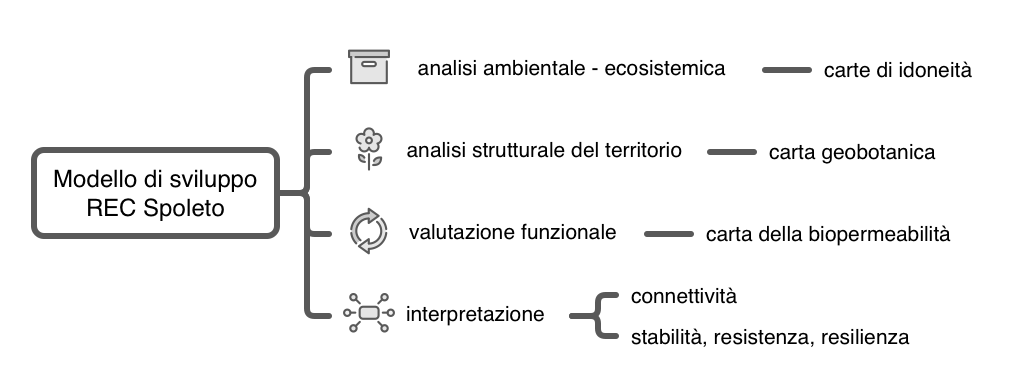
\includegraphics[keepaspectratio]{./figs/RECSpoleto_map03.png}}
\caption{Figura 2.1 - Scheda delle fasi di lavoro e risultati cartografici attesi.}
\end{figure}

\subsection{Sviluppo banca dati faunistica}\label{sviluppo-banca-dati-faunistica}

In primo luogo sono state individuate le fonti più utili per inquadrare lo stato del territorio e descrivere le sue caratteristiche ecosistemiche.
Tra queste, per estrapolare il quadro conoscitivo faunistico essenziale per la definizione delle future carte di idoneità, sono state utilizzate le informazioni pubblicate negli atlanti faunistici regionali, le schede dei formulari standard di Natura 2000 che riportano in dettaglio le caratteristiche aggiornate dei siti e delle loro comunità e le osservazioni contenute nelle banche dati sviluppate secondo la filosofia ``\emph{Free and open access to biodiversity data}''.

Le informazioni raccolte hanno contribuito alla caratterizzazione della biodiversità locale e alla redazione della lista di specie presenti.
L'inventario è costituito prevalentemente da specie di vertebrati, ma è stato integrato con osservazioni occasionali di invertebrati provenienti da banche dati aperte.
Queste informazioni, sebbene non derivino da monitoraggi sistematici, concorrono a delineare un quadro conoscitivo aggiornato della fauna comunale, restituendo seppur parzialmente anche il ruolo della componente invertebrata, di cui localmente si hanno scarse conoscenze distributive.
Pertanto, benché tali dati siano lontani dal rappresentare l'effettiva ricchezza specifica (in Italia la fauna invertebrata costituisce circa il 98\% della fauna totale\footnote{La fauna italiana (marina, terrestre e d'acqua dolce) è stimata in oltre 60.000 specie, di cui circa il 98\% costituito da Invertebrati e il rimanente da circa 1.300 specie di Vertebrati.
  Il phylum più ricco è quello degli Artropodi, con quasi 50.000 specie, in buona parte appartenenti alla classe degli Insetti, in particolare Coleotteri (12.000 specie circa).}), essi offrono comunque un contributo significativo alla caratterizzazione faunistica del territorio.

\subsection{Carta geobotanica}\label{carta-geobotanica}

Per l'avanzamento del progetto Rete Ecologica Comunale è stato predisposto un programma di aggiornamento e revisione della garta geobotanica e di uso del suolo dell'intero territorio comunale.
La base di partenza è rappresentata dalla carta geobotanica sviluppata per il territorio regionale umbro nel 2018 per il progetto RERU3 che era stata realizzata con scala nominale pari a 1:10.000 con un dettaglio cartografico pari a circa un ettaro, ridotto a 2.000 metri quadrati per le formazioni boscate e a 5.000 metri quadrati per gli impianti di arboricoltura da legno, e una precisione pari a circa 5 m.

L'importanza di disporre di una carta geobotanica e dell'uso del suolo dettagliata e aggiornata risiede nel suo valore strategico per molteplici ambiti di applicazione scientifica e gestionale.
Dal punto di vista scientifico-ecologico riveste una notevole rilevanza poiché consente di valutare il grado di naturalità del territorio e conseguentemente anche l'identificazione dei pattern di biodiversità e delle aree di particolare valore naturalistico.
Sul piano della pianificazione gestionale, disporre di una cartografia dettagliata e aggiornata che tenga conto della distribuzione spaziale delle comunità vegetali e delle infrastrutture antropiche facilita le analisi necessarie per l'applicazione delle norme ambientali, la valutazione degli impatti derivanti da interventi antropici e per orientare le scelte nella loro fase di pianificazione e progettazione.

Nell'ambito dello studio in oggetto, questa carta è stata realizzata utilizzando il sistema di riferimento in coordinate piane EPSG:3035 (ETRS89-extended / LAEA Europe).
Un contributo significativo all'aggiornamento di questa carta è stato dato dai volontari del servizio civile presso il Dipartimento 8 - Transizione ecologica economia circolare nel periodo 2024-2025.
Non solo, per lo sviluppo della carta sono stati impegnati anche numerosi studenti delle scuole secondarie di secondo grado della città di Spoleto che nell'ambito delle loro attività PCTO con questa carta hanno testato le loro competenze in materia di software GIS e acquisito conoscenze pratiche nell'analisi territoriale, nella cartografia digitale e nelle metodologie di rilevamento ambientale.

Per descrivere le caratteristiche generali di questa carta sono state utilizzate metriche del paesaggio elaborate utilizzando il software FRAGSTATS (\url{https://www.fragstats.org}).
Con questo software è possibile calcolare diversi indici spaziali che quantificano la composizione e la configurazione del paesaggio, permettendo di analizzare la frammentazione degli habitat, la connettività ecologica e la diversità strutturale del territorio analizzato.
FRAGSTATS è infatti uno dei software più utilizzati nell'analisi del paesaggio per:

\begin{itemize}
\tightlist
\item
  Calcolare indici di frammentazione
\item
  Valutare la diversità e l'eterogeneità spaziale
\item
  Analizzare le patch (tessere) del paesaggio
\item
  Misurare la connettività tra habitat
\item
  Quantificare i margini e le zone di ecotono
\end{itemize}

In particolare, le metriche esaminate sono state:

\begin{itemize}
\tightlist
\item
  \textbf{Land cover}: è una metrica semplice, nota anche come area totale, identifica l'area totale coperta da ogni classe;
\item
  \textbf{Landscape proportion (PLAND)}: indica la percentuale dell'area di una classe rispetto all'area totale. È una misura importante in quanto permette di comprendere immediatamente quali sono le classi dominanti;
\item
  \textbf{Number of patches (NP)}: è una delle metriche più semplici e ci restituisce il numero totale di patches che compongono il paesaggio. NP = 1 quando siamo in presenza di una sola patch; quando siamo in presenza di habitat altamente frammentato e sottoposto a sprawl urbano il numero di patches è elevato.
\item
  \textbf{Mean patch area (MPA)}: indica la dimensione media delle patch, più le patches delle varie classi hanno una dimensione simile più i valori si assomigliano. Qualora si presentassero evidenti differenze di valore significa che siamo di fronte a un territorio eterogeneo;
\item
  \textbf{Edge density (ED)}: è la lunghezza di tutti bordi di una classe in relazione all'area totale di ogni classe del paesaggio. Il valore è uguale a 0 se è presente una sola patch, e cresce all'aumentare della frammentazione del paesaggio;
\item
  \textbf{Largest Patch Index (LPI)}: è uguale all'area della patch più grande di ogni tipo di classe del suolo;
\item
  \textbf{Fractal Dimension Index}: è una ``metrica della forma'', si basa sul perimetro della patch e sull'area della patch e descrive la complessità della patch;
\item
  \textbf{Patch Cohesion Index}: esprime il grado di connessione naturale tra i tipi di paesaggio, un numero vicino allo zero indica che la classe è molto frammentata mentre un numero alto indica che sono molto collegate.
\end{itemize}

\subsection{Carta di idoneità generale}\label{carta-di-idoneituxe0-generale}

La valutazione della funzionalità territoriale rispetto agli spostamenti faunistici richiede come primo step un'analisi dell'idoneità ambientale, definita anche come vocazionalità, che rappresenta la misura di quanto un determinato ambiente sia adatto a sostenere una specie o una comunità biologica.
Questo concetto quantifica la capacità di un habitat di fornire le risorse e le condizioni necessarie per la sopravvivenza, la crescita e la riproduzione di quel particolare organismo, di una popolazione o di un'intera comunità.
Nella pratica scientifica e gestionale, l'idoneità o ``\emph{habitat suitability}'' viene spesso espressa attraverso modelli matematici che assegnano valori numerici (generalmente compresi tra 0 e 1, dove 0 indica completa inadeguatezza e 1 massima idoneità) a diverse porzioni del territorio.

Nel caso in esame, la carta di idoneità è stata elaborata a titolo esplorativo sulla base delle esigenze biologiche ed ecologiche del set di specie di vertebrati precedentemente selezionati per l'elaborazione della rete ecologica regionale (cfr. RERU) e tenendo conto delle categorie di uso del suolo aggiornate nel contesto comunale con la carta geobotanica.
Per la realizzazione di questa carta generale sono stati impiegati dei modelli geostatistici a massima entropia noti anche come \emph{Species Distribution Models} (SDM) in grado di quantificare la vocazionalità territoriale sulla base delle categorie ambientali (cfr. Maxent ==BIB==).
Lo scopo finale di questi strumenti modellistici è quello di mappare e quantificare il potenziale biologico del territorio, fornendo una base scientifica per comprendere come le diverse aree possano supportare la presenza e gli spostamenti della fauna locale o per supportare i processi di pianificazione territoriale, soprattutto quelli mirati alla conservazione della biodiversità e alla valutazione degli impatti ambientali.

\subsection{Carta della permeabilità}\label{carta-della-permeabilituxe0}

Dopo aver valutato le potenzialità del territorio alla presenza delle specie è necessario trasformare questo valore in un indicatore più vicino alla realtà attraverso la valutazione degli elementi del territorio che possono influenzare la capacità di spostamento delle specie nel territorio.
La distribuzione spaziale delle risorse nel paesaggio è infatti organizzata sotto forma di patch discrete e affinché il territorio sia caratterizzato da processi ecologici funzionali è necessario assicurare il movimento degli animali tra le diverse aree dove sono presenti tali risorse (Taylor et al.~1993).
Alcuni elementi limitano o impediscono il passaggio della fauna da una zona all'altra, mentre altri agevolano la mobilità e il trasferimento degli individui delle popolazioni.
Nel primo caso si parla di barriere (spesso codificate come infrastrutture grigie) mentre nel secondo caso di corridoi (infrastrutture verdi e blu).
Le infrastrutture antropiche spesso costituiscono le forme di barriere più significative.
Le strade, soprattutto quelle ad alto traffico sono un esempio di ostacolo particolarmente critico, non solo per la mortalità diretta legata agli investimenti veicolari, ma anche per l'effetto barriera esercitato dal rumore, l'inquinamento luminoso e le vibrazioni associate al transito dei mezzi.
I corridoi ecologici sono invece quegli elementi lineari del paesaggio che facilitano il movimento degli organismi tra habitat, mantenendo la connettività funzionale del territorio.
Questi elementi possono essere di diversa natura e scala, dalla semplice siepe che collega due frammenti di habitat fino ai più grandi corridoi fluviali.
In particolare, i sistemi fluviali e le loro fasce ripariali rappresentano le più importanti vie di connettività poiché la loro vegetazione offre a un gran numero di specie copertura, risorse alimentari e microhabitat diversificati (==BIB==).
Anche il sistema costituita da parchi, giardini, viali alberati e tetti verdi, possono creare connessioni importanti per alcune specie in grado di adattarsi agli ambienti antropizzati.
Allo stesso tempo anche le coltivazioni gestite con pratiche sostenibili, possono assicurare un buon grado di permeabilità per la fauna, mantenendo inalterato il loro valore produttivo.

\subsection{Analisi della Frammentazione}\label{analisi-della-frammentazione}

La frammentazione territoriale costituisce un fenomeno complesso caratterizzato dalla progressiva riduzione della superficie degli ecosistemi naturali e seminaturali, accompagnata da un crescente isolamento spaziale delle aree residue (==BIB==).
Questo processo di disgregazione paesaggistica determina la trasformazione del territorio in mosaici frammentati, composti da tessere di habitat di dimensioni ridotte e spazialmente disgiunte.
Associati a questo tipo di paesaggio ci sono diversi tipi di rischi che ne compromettono la funzionalità ecologica.
A livello di popolazione, generalmente il processo di frammentazione aumenta il grado di vulnerabilità: popolazioni piccole e isolate sono infatti soggette a deriva genetica, perdita di variabilità genetica e depressione da inbreeding, tutti fenomeni che riducono la fitness individuale e la capacità di adattamento.
Nei casi più severi comporta anche una riduzione dell'efficacia della dispersione, compromettendo la dinamica metapopolazionale e aumentando il rischio di estinzioni locali.
Ulteriore fattore di rischio è inoltre, l'effetto margine che, attraverso l'incremento del rapporto perimetro/area delle patches, espone porzioni crescenti di habitat alle condizioni microclimatiche alterate dei margini.
Alcuni esempi di questi effetti includono le modificazioni delle condizioni di luce, della temperatura, dell'umidità e della penetrazione del vento, che possono alterare in modo cruciale la composizione specifica, la struttura delle comunità biologiche e conseguentemente la loro capacità di fornire servizi ecosistemici essenziali.
I principali motori di questa trasformazione sono rappresentati dai processi di urbanizzazione e dalla sottrazione di habitat naturali.
In particolare, quelli che si manifestano attraverso varie modalità di sviluppo territoriale e dall'espansione della rete infrastrutturale.
Associato al concetto della frammentazione c'è il suo complemento ovvero la connettività.
Questa è definita come ``il grado in cui il paesaggio facilita il movimento di risorse tra le aree'' e può essere misurata dalla probabilità di movimento tra tutti i punti o le aree di habitat in un paesaggio (Taylor et al., 1993).

Per una prima valutazione del livello di frammentazione del territorio sono stati calcolati tre indici generali, che rappresentano misure complementari, ciascuna con specifiche proprietà e interpretazioni (Jaeger 2000).
In particolare sono stati considerati, ripartendoli a livello di unità di paesaggio,: il landscape division, lo splitting index e l'effective mesh size.

Il \emph{landscape division} (divisione del paesaggio - D) è definito come la probabilità che due punti scelti casualmente all'interno del paesaggio non siano connessi a causa della frammentazione.
Questo indice varia da 0 (paesaggio completamente connesso) a valori prossimi a 1 (paesaggio completamente frammentato).
La divisione del paesaggio fornisce una misura intuitiva del grado di isolamento strutturale, quantificando la perdita di connettività dovuta alla presenza di barriere antropiche.
Dal punti di vista matematico il calcolo di questo indice si basa sull'equazione:

\[C=1-\sum_{i=1}^{n}(A_i/A_t)^2\]

dove:

\begin{itemize}
\tightlist
\item
  \(C\) = indice di frammentazione
\item
  \(A_i\) = area del patch i-esimo
\item
  \(A_t\) = area totale del paesaggio
\item
  \(n\) = numero totale di patches
\end{itemize}

Lo \emph{splitting index} (indice di suddivisione - S) rappresenta il numero di patches di uguale dimensione in cui il paesaggio dovrebbe essere diviso per ottenere lo stesso grado di frammentazione di quello osservato.
Questo indice assume valori compresi tra 1 (paesaggio non frammentato) e il numero totale di patches nel caso di frammentazione estrema.
Lo splitting index è particolarmente utile per confrontare il grado di frammentazione tra paesaggi di dimensioni diverse, poiché standardizza l'effetto della scala spaziale.
Dal punto di vista matematico il calcolo di questo indice si basa sull'equazione:

\[S=\frac{A_{t}^{2}}{\sum_{i=1}^{n}A_i^2}\]

dove:

\begin{itemize}
\tightlist
\item
  \(S\) = splitting index
\item
  \(A_t\) = area totale del paesaggio
\item
  \(A_i\) = area del patch i-esimo
\item
  \(n\) = numero totale di patches
\end{itemize}

Lo splitting index può anche essere espresso in relazione al landscape division (D) come:

\[S=\frac{1}{1-D}\]

L'\emph{effective mesh size} (dimensione effettiva delle maglie) rappresenta la dimensione che avrebbero le patches se il paesaggio fosse suddiviso in un numero di elementi di uguale area corrispondente al grado di frammentazione osservato.
Questo parametro è espresso in unità di superficie e diminuisce all'aumentare della frammentazione.
L'effective mesh size fornisce un'indicazione diretta della scala spaziale alla quale operano i processi ecologici in un paesaggio frammentato, rappresentando una misura della ``granularità'' strutturale del mosaico paesaggistico.
Nella sua formulazione matematica questo indice viene calcolato attraverso l'equazione:

\[m_{eff} = \frac{1}{A_t} \sum_{i=1}^{n} A_i^2\]

dove: - \(m_{eff}\) = effective mesh size - \(A_t\) = area totale del paesaggio - \(A_i\) = area del patch i-esimo - n = numero totale di patches

L'effective mesh size può anche essere espressa in relazione allo splitting index (S) come:

\[m_{eff} = \frac{A_t}{S}\]

Queste tre metriche tradizionali in alcuni casi possono presentare delle valutazioni leggermente distorte, soprattutto quando i confini delle unità di studio frammentano artificialmente le patch naturali.
Questo fenomeno, noto come ``\emph{boundary problem}'', può portare a valutazioni errate della frammentazione del paesaggio, poiché patch che in realtà sono continue vengono considerate separate semplicemente perché attraversano i confini dell'area di studio.
Per superare questa limitazione Moser et al.~(2007), hanno proposto il metodo Cross-Boundary Connections (CBC).
Questo approccio affronta la limitazione includendo nell'analisi anche le aree esterne ai confini dell'unità di studio.
L'approccio si basa su un principio fondamentale: considerare l'area completa di ogni patch (\(A^{cmpl}_i\)), indipendentemente dai confini amministrativi o metodologici dell'area di indagine.

Sulla base anche di quest'ultima variate metodologica sono state eseguite alcune valutazioni sulle unità di paesaggio e sull'intero territorio comunale considerando tutte le fasce altitudinali e la sola fascia del piano collinare compreso tra i 200 e i 400 m s.l.m.

\subsection{Morphological Spatial Pattern Analysis}\label{morphological-spatial-pattern-analysis}

L'analisi dei pattern morfologici spaziali o \emph{Morphological Spatial Pattern Analysis} (MSPA) identifica una metodologia di analisi spaziale sviluppata dal Joint Research Centre (JRC) della Commissione Europea e disponibile attraverso un codice in formato aperto (Vogt and Riitters, 2017).
Questo approccio analitico ha trovato applicazione in contesti istituzionali di rilievo, tra cui i rapporti ufficiali dell'USDA-Forest Service per il monitoraggio dello stato delle foreste e delle praterie, nonché nell'ambito del programma EnviroAtlas dell'EPA. Il processo algoritmico MSPA genera una mappa di sintesi che fornisce un quadro statistico completo dei pattern spaziali ambientali presenti nell'area di studio.
Questa rappresentazione cartografica integra diverse tipologie di classi morfologiche e identifica i corridoi di connessione ecologica presenti nel territorio.\\
Il framework metodologico si basa su un sistema di operatori matematico-morfologici progettati per caratterizzare le geometrie spaziali e le relazioni di connettività presenti nella carta di uso del suolo.
Si tratta di un processo di segmentazione dei dati di input e non genera nuovi pattern rispetto alle categorie già presenti nelle carte di partenza.
Le categorie fondamentali di classificazione includono: Core (aree centrali di habitat), Isole (frammenti isolati), Perforazioni (aperture all'interno di aree core), Margini (zone di transizione), Anelli (connessioni circolari), Ponti (elementi di connessione lineare tra zone di habitat) e Rami (elementi di connessione che terminano nella matrice di background).
Tutto ciò che nella mappa non viene identificato come ``habitat'' o foreground viene assegnato alla tipologia background e suddiviso in tre possibili tipologie: Core-opening (aree di background all'interno delle aree core), background di margine (aree di background adiacenti ai margini dell'habitat) e zone esterne (non in contatto diretto con l'habitat).
La metodologia si basa esclusivamente su principi geometrici e quelli degli insiemi matematici.
In quanto tale, può essere applicata a qualsiasi tipo di mappa raster di uso del suolo, indipendentemente dalla definizione delle singole categorie e dalla risoluzione spaziale della mappa analizzata.
Con questo approccio si ottiene un maggior numero di statistiche sugli elementi modellati e un risultato cartografico spazialmente esplicito che include i percorsi di connessione tra le aree core individuate nel modello del territorio.

Nella configurazione di base per poter procedere con una modellazione devono essere settati 4 parametri:

- \textbf{connettività} (foreground connectivity).
Ci sono due possibili opzioni: una connettività a 8 celle, in cui a partire da una prima cella gli spostamenti sono consentiti in tutte le direzioni dello spazio, incluse diagonali e angoli; in alternativa si può utilizzare una connettività a 4 celle, in cui sono ammessi collegamenti soltanto per celle con un bordo in comune.

- \textbf{spessore del margine} (edge width), in cui si definisce l'estensione dei margini delle aree core sotto forma di aree di buffer.

- presenza (1) o assenza (0) di \textbf{zone di transizione} che attraversano le zone di margine.

- intext (0,1), che permette di separare le \textbf{porzioni esterne e interne}, dove le caratteristiche interne sono quelle racchiuse da una perforazione.

\subsection{Marxan}\label{marxan}

Per consolidare il sistema della rete ecologica tra gli strumenti che verranno impiegati dal software Marxan (==BIB==).
Marxan è stato sviluppato per la progettazione di un sistema connesso di aree ad alta valenza naturalistica soddisfacendo il requisito di ``minimo costo'' in un complesso di scenari multipli.
Nel contesto della progettazione il costo minimo può riferirsi a quell'insieme di valutazioni di natura ecologica, sociale ed economiche finalizzate a ottenere una rappresentazione minima delle caratteristiche della biodiversità con il minor costo possibile.
La logica è che è più probabile che vengano mantenuti gli elementi della rete se questi si dimostrano essere i più economici o i meno socialmente dirompenti.
Lo scopo dell'utilizzo di questo set di algoritmi risiede nell'importanza di supportare il processo decisionale e fornire un punto di partenza solido e riproducibile per le discussioni sulla pianificazione.
I risultati finali dovranno poi essere perfezionati dai decisori che hanno il compito di considerare l'intera gamma di fattori politici, socio-economici e pratici che influenzano l'attuazione della pianificazione.

\chapter{Risultati}\label{risultati}

\section{Quadro conoscitivo di base}\label{quadro-conoscitivo-di-base}

Il comune di Spoleto si sviluppa su una superficie di 349,2 \(km^2\), in un range altitudinale compreso tra i 220 e i 1337 m s.l.m (la cima più alta è M. Fionchi nella porzione sud orientale del comune)(Fig. \ref{fig:cartaSpoleto}).
L'area comprende 8 siti Natura 2000 che si estendono per 3441.77 ha, occupando una superficie pari al 9.8\% del totale.
Due di questi sono interamente compresi nei confini comunali (IT5210069 -- Boschi di Montebibico (Monti Martani) e IT5210064 -- Monteluco di Spoleto), mentre gli altri sono condivisi con i comuni limitrofi (Tab. \ref{tab:sitiN2k}).

\begin{figure}

{\centering 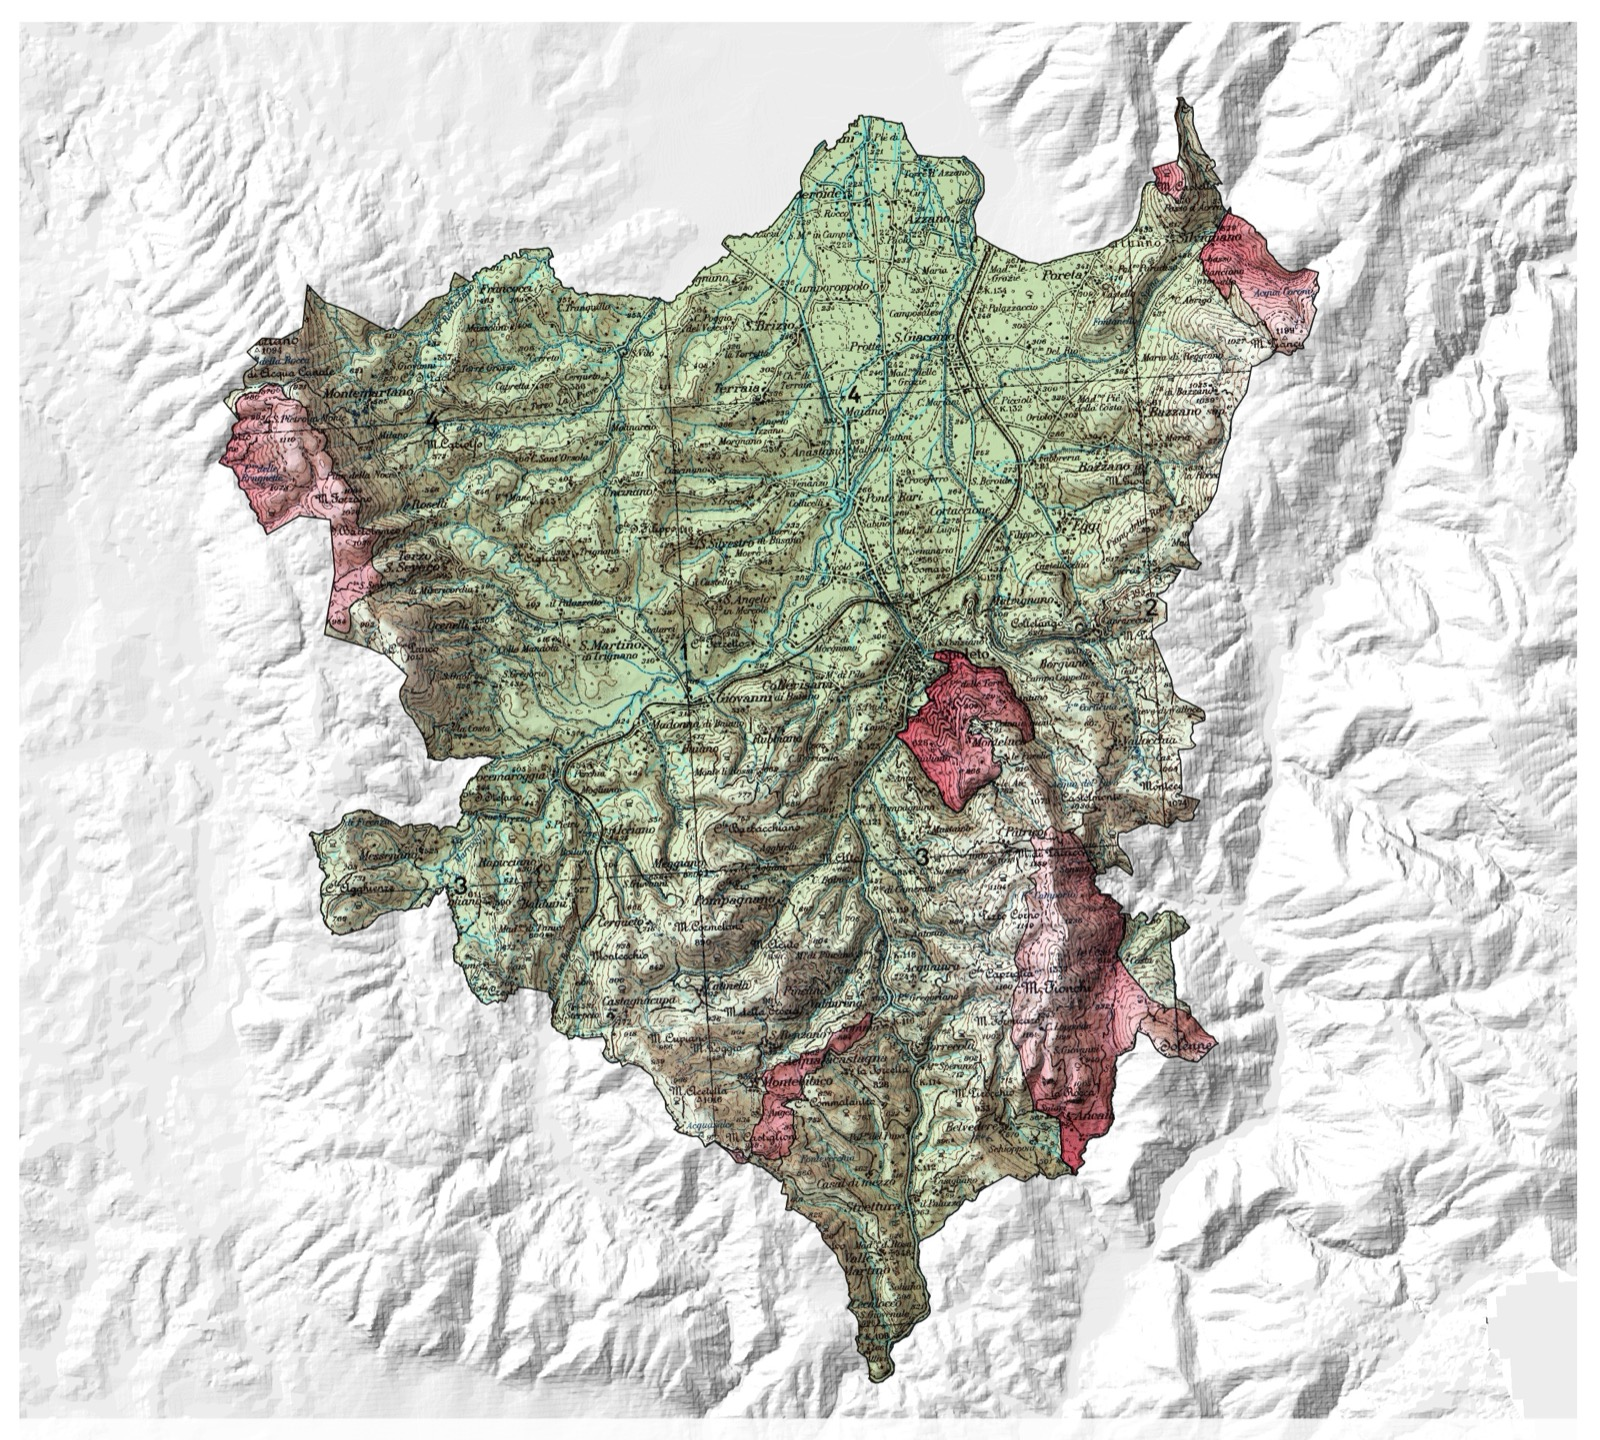
\includegraphics[width=\linewidth]{./figs/RECSpoleto_map01} 

}

\caption{Il territorio spoletino. In tonalità rosse sono evidenziate le aree Natura 2000.}\label{fig:cartaSpoleto}
\end{figure}

\begin{longtable}[]{@{}
  >{\raggedright\arraybackslash}p{(\linewidth - 8\tabcolsep) * \real{0.2000}}
  >{\raggedright\arraybackslash}p{(\linewidth - 8\tabcolsep) * \real{0.2000}}
  >{\centering\arraybackslash}p{(\linewidth - 8\tabcolsep) * \real{0.2000}}
  >{\centering\arraybackslash}p{(\linewidth - 8\tabcolsep) * \real{0.2000}}
  >{\centering\arraybackslash}p{(\linewidth - 8\tabcolsep) * \real{0.2000}}@{}}
\caption{\label{tab:sitiN2k} Siti Natura 2000 presenti nel Comune di Spoleto e relative superfici espresse in ha e valore percentuale.}\tabularnewline
\toprule\noalign{}
\begin{minipage}[b]{\linewidth}\raggedright
\textbf{Codice sito}
\end{minipage} & \begin{minipage}[b]{\linewidth}\raggedright
\textbf{Nome sito}
\end{minipage} & \begin{minipage}[b]{\linewidth}\centering
\textbf{Tipologia}
\end{minipage} & \begin{minipage}[b]{\linewidth}\centering
\textbf{Superficie}
\end{minipage} & \begin{minipage}[b]{\linewidth}\centering
\textbf{Superficie comune}
\end{minipage} \\
\midrule\noalign{}
\endfirsthead
\toprule\noalign{}
\begin{minipage}[b]{\linewidth}\raggedright
\textbf{Codice sito}
\end{minipage} & \begin{minipage}[b]{\linewidth}\raggedright
\textbf{Nome sito}
\end{minipage} & \begin{minipage}[b]{\linewidth}\centering
\textbf{Tipologia}
\end{minipage} & \begin{minipage}[b]{\linewidth}\centering
\textbf{Superficie}
\end{minipage} & \begin{minipage}[b]{\linewidth}\centering
\textbf{Superficie comune}
\end{minipage} \\
\midrule\noalign{}
\endhead
\bottomrule\noalign{}
\endlastfoot
IT5210050 & Valle di Pettino (Campello sul Clitunno) & B & 844.3 & 42.3 \\
IT5210057 & Fosso di Camposolo & B & 609.2 & 377.1 \\
IT5210060 & Monte Il Cerchio (Monti Martani) & B & 1595.8 & 734.4 \\
IT5210064 & Monteluco di Spoleto & B & 504.3 & 504.3 \\
IT5210069 & Boschi di Montebibico (Monti Martani) & B & 215.4 & 215.4 \\
IT5220010 & Monte Solenne (Valnerina) & B & 921.0 & 121.9 \\
IT5220014 & Valle del Serra (Monti Martani) & B & 1274.7 & 8.7 \\
IT5220025 & Bassa Valnerina: Monte Fionchi - Cascata delle Marmore & A & 6372.0 & 1437.6 \\
\end{longtable}

\subsection{Dati Faunistici}\label{dati-faunistici}

Dall'analisi delle schede del formulario standard delle aree Natura 2000 emerge che nel territorio comunale sono presenti 113 specie di interesse comunitario, incluse negli allegati II, IV e V della Direttiva Habitat (DIRETTIVA 92/43/CEE) ripartite nei gruppi faunistici di Tab.
\ref{tab:DH}:

\begin{longtable}[]{@{}lc@{}}
\caption{\label{tab:DH} Numero di specie incluse negli allegati della Direttiva Habitat (fonte: eunis.eu)}\tabularnewline
\toprule\noalign{}
Gruppo faunistico & numero di specie \\
\midrule\noalign{}
\endfirsthead
\toprule\noalign{}
Gruppo faunistico & numero di specie \\
\midrule\noalign{}
\endhead
\bottomrule\noalign{}
\endlastfoot
Invertebrati & 3 \\
Pesci & 1 \\
Anfibi & 3 \\
Rettili & 2 \\
Uccelli & 97 \\
Mammiferi & 6 \\
TOTALE & 113 \\
\end{longtable}

A questo gruppo particolare di specie se ne aggiungono ulteriori 183 annoverate nella categoria di ``altre specie'' che portano complessivamente la ricchezza specifica totale a 296 specie (Tab. \ref{tab:DHaltre}).

\begin{longtable}[]{@{}lc@{}}
\caption{\label{tab:DHaltre} Numero di specie incluse nei formulari standard dei siti Natura 2000 ricompresi nel territorio comunale (fonte: eunis.eu).}\tabularnewline
\toprule\noalign{}
Gruppo faunistico & numero di specie \\
\midrule\noalign{}
\endfirsthead
\toprule\noalign{}
Gruppo faunistico & numero di specie \\
\midrule\noalign{}
\endhead
\bottomrule\noalign{}
\endlastfoot
Invertebrati & 8 \\
Pesci & 8 \\
Anfibi & 10 \\
Rettili & 15 \\
Uccelli & 106 \\
Mammiferi & 36 \\
TOTALE & 183 \\
\end{longtable}

Considerando i dati pubblicati attraverso gli atlanti regionali e le ulteriori informazioni validate e conservate presso l'Osservatorio Faunistico Regionale di Regione Umbria che ha gentilmente messo a disposizione la banca dati, il quadro che ne deriva per il comune di Spoleto relativamente al gruppo dei vertebrari presenta 192 specie, ripartiti in 5 gruppi (Tab. \ref{tab:ofr}).

\begin{longtable}[]{@{}lc@{}}
\caption{\label{tab:ofr} Numero di specie rilevate e validate presenti nella banca dati dell'Osservatorio Faunistico Regionale (Regione Umbria).}\tabularnewline
\toprule\noalign{}
Gruppo faunistico & numero di specie \\
\midrule\noalign{}
\endfirsthead
\toprule\noalign{}
Gruppo faunistico & numero di specie \\
\midrule\noalign{}
\endhead
\bottomrule\noalign{}
\endlastfoot
Anfibi & 9 \\
Rettili & 11 \\
Uccelli & 133 \\
Mammiferi & 41 \\
TOTALE & 192 \\
\end{longtable}

Consultando infine le osservazioni documentate e validate dalla banca dati \href{https://www.gbif.org}{gbif} (aggiornata al febbraio 2025) il patrimonio faunistico si arricchisce di ulteriori 1310 osservazioni relative a 13 classi animali per una ricchezza specifica di 388 specie.

\begin{longtable}[]{@{}lc@{}}
\toprule\noalign{}
Gruppo faunistico (classe) & numero di specie \\
\midrule\noalign{}
\endhead
\bottomrule\noalign{}
\endlastfoot
Amphibia & 7 \\
Arachnida & 16 \\
Aves & 110 \\
Cestoda & 13 \\
Chilopoda & 3 \\
Clitellata & 2 \\
Crustacea & 1 \\
Diplopoda & 5 \\
Gastropoda & 32 \\
Insecta & 184 \\
Mammalia & 5 \\
Squamata & 8 \\
Trematoda & 2 \\
TOTALE & 388 \\
\end{longtable}

Mettendo a sistema l'intero set di dati faunistici la sintesi che ne emerge è rappresentata in figura \ref{fig:faunaSpoletoAll} in cui il numero finale di taxa è pari a 533 con una ripartizione al 50\% tra vertebrati e invertebrati.

\begin{figure}

{\centering 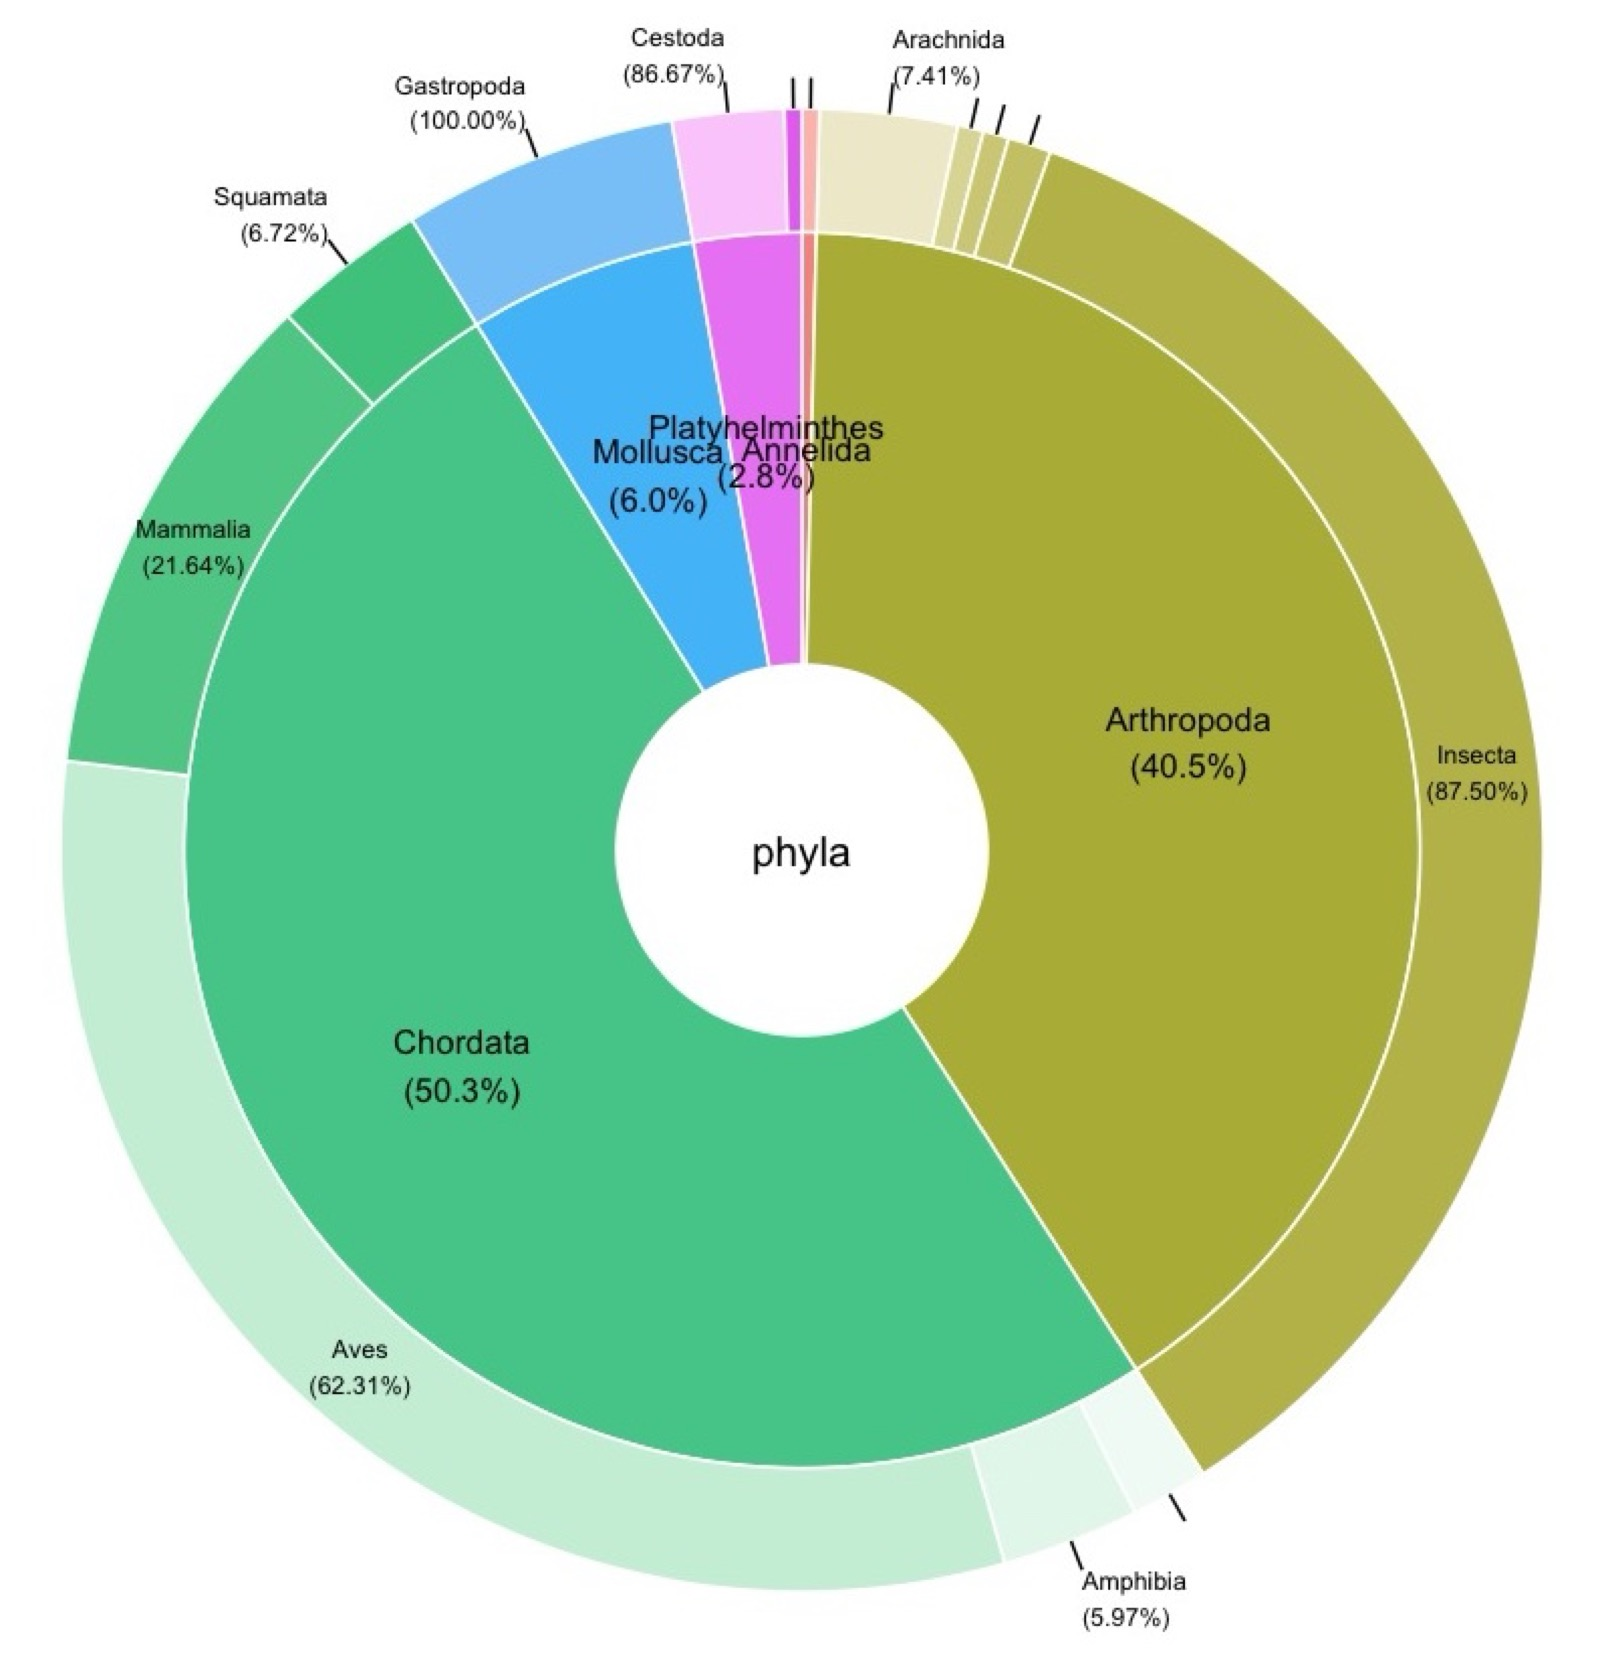
\includegraphics[width=\linewidth]{./figs/faunaSpoletoAll} 

}

\caption{Distribuzione percentuale delle diverse specie disaggregate per Phylum e per Classe.}\label{fig:faunaSpoletoAll}
\end{figure}

Analizzando la distribuzione delle specie per classe zoologica in entrambi i gruppi esaminati, si nota una netta predominanza di due categorie: insetti e uccelli (Fig. \ref{fig:faunaperc}).
Nel territorio comunale sono state finora documentate 189 specie di insetti e 161 specie di uccelli.
Questi due gruppi rappresentano insieme più di due terzi della biodiversità attualmente conosciuta nell'area.
È importante sottolineare, però, che il grado di completezza dei dati varia significativamente tra le due classi.
Per quanto riguarda gli uccelli è ragionevole supporre che il numero di specie registrate si avvicini molto alla ricchezza reale presente nel territorio.
Al contrario, per gli insetti la situazione è molto diversa: le 189 specie catalogate rappresentano solo una piccola frazione della diversità effettiva, con un numero molto elevato di specie ancora da identificare e studiare.

\begin{figure}

{\centering 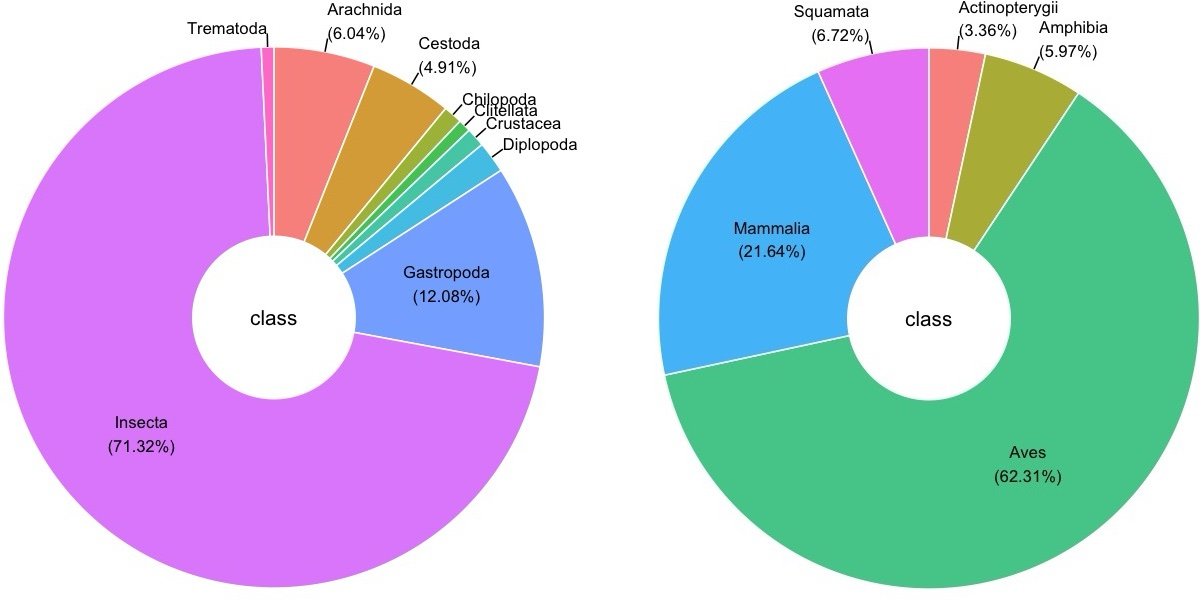
\includegraphics[width=\linewidth]{./figs/faunaSpoletoInv} 

}

\caption{Distribuzione percentuale delle specie animali disaggregate per classe tra inverbetrati (sinistra) e vertebrati (destra).}\label{fig:faunaperc}
\end{figure}

\section{Elaborazioni cartografiche}\label{elaborazioni-cartografiche}

\subsection{Carta geobotanica}\label{carta-geobotanica-1}

Complessivamente nel territorio spoletino sono state codificate 29 differenti patches di categorie geobotaniche e di uso del suolo (Fig. \ref{fig:ortogeo} e Tab.
\ref{tab:geobot}).

\begin{figure}

{\centering \includegraphics[width=\linewidth]{./figs/ortogeo} 

}

\caption{Ortofotocarta e Carta geobotanica e di uso del suolo aggiornata per il comune di Spoleto.}\label{fig:ortogeo}
\end{figure}

\begin{longtable}[]{@{}
  >{\centering\arraybackslash}p{(\linewidth - 6\tabcolsep) * \real{0.2500}}
  >{\raggedright\arraybackslash}p{(\linewidth - 6\tabcolsep) * \real{0.2500}}
  >{\centering\arraybackslash}p{(\linewidth - 6\tabcolsep) * \real{0.2500}}
  >{\centering\arraybackslash}p{(\linewidth - 6\tabcolsep) * \real{0.2500}}@{}}
\caption{\label{tab:geobot} Categorie geobotaniche e uso del suolo presenti nel territorio spoletino ordinate in modo decrescente in relazione alla loro estensione.}\tabularnewline
\toprule\noalign{}
\begin{minipage}[b]{\linewidth}\centering
Classe
\end{minipage} & \begin{minipage}[b]{\linewidth}\raggedright
Categoria geobotanica
\end{minipage} & \begin{minipage}[b]{\linewidth}\centering
superficie (\(km^2\))
\end{minipage} & \begin{minipage}[b]{\linewidth}\centering
area (\%)
\end{minipage} \\
\midrule\noalign{}
\endfirsthead
\toprule\noalign{}
\begin{minipage}[b]{\linewidth}\centering
Classe
\end{minipage} & \begin{minipage}[b]{\linewidth}\raggedright
Categoria geobotanica
\end{minipage} & \begin{minipage}[b]{\linewidth}\centering
superficie (\(km^2\))
\end{minipage} & \begin{minipage}[b]{\linewidth}\centering
area (\%)
\end{minipage} \\
\midrule\noalign{}
\endhead
\bottomrule\noalign{}
\endlastfoot
22 & 022 Boschi di caducifoglie collinari e submontane & 144.4 & 41.3 \\
141 & 141 Seminativi semplici & 84.7 & 24.2 \\
160 & 160 Oliveti & 24.2 & 6.9 \\
91 & 091 Praterie secondarie submediterranee & 23.0 & 6.6 \\
200 & 200 Aree urbanizzate & 20.6 & 5.9 \\
11 & 011 Boschi di sclerofille mediterranee & 15.7 & 4.5 \\
12 & 012 Pinete mediterranee & 7.3 & 2.1 \\
70 & 070 Filari e Siepi & 5.2 & 1.5 \\
61 & 061 Arbusteti collinari & 2.9 & 0.8 \\
151 & 151 Seminativi arborati & 2.8 & 0.8 \\
170 & 170 Vigneti & 3.0 & 0.8 \\
191 & 191 Arboricoltura da legno & 2.9 & 0.8 \\
130 & 130 Rimboschimenti & 2.4 & 0.7 \\
23 & 023 Castagneti da frutto e Boschi di castagno & 2.0 & 0.6 \\
40 & 040 Boschi e boscaglie di caducifoglie ripariali & 1.9 & 0.6 \\
94 & 094 Praterie secondarie calanchive & 1.5 & 0.4 \\
31 & 031 Boschi di caducifoglie montane & 0.7 & 0.2 \\
101 & 101 Vegetazione idrofitica lacustre & 0.7 & 0.2 \\
142 & 142 Campi abbandonati e incolti & 0.6 & 0.2 \\
152 & 152 Colture agrarie mosaicizzate & 0.7 & 0.2 \\
92 & 092 Praterie secondarie montane & 0.5 & 0.1 \\
93 & 093 Praterie secondarie di fondovalle & 0.2 & 0.1 \\
102 & 102 Vegetazione idrofitica fluviale & 0.3 & 0.1 \\
111 & 111 Popolamenti terofitici & 0.4 & 0.1 \\
210 & 210 Aree con vegetazione scarsa o nulla & 0.5 & 0.1 \\
52 & 052 Brughiere (basso) collinari & 0.1 & 0.0 \\
62 & 062 Arbusteti montani & 0.2 & 0.0 \\
120 & 120 Vegetazione casmofitica & 0.0 & 0.0 \\
180 & 180 Frutteti & 0.1 & 0.0 \\
\end{longtable}

Dall'analisi della carta risulta che il territorio è coperto per circa il 46\% da boschi (di cui la maggior parte 41.3\% di caducifoglie), il 24.2\% da aree agricole con seminativi semplici, il 7\% da oliveti e meno del 6\% da aree urbanizzate (Fig. \ref{fig:usoSuolo}).

\begin{figure}
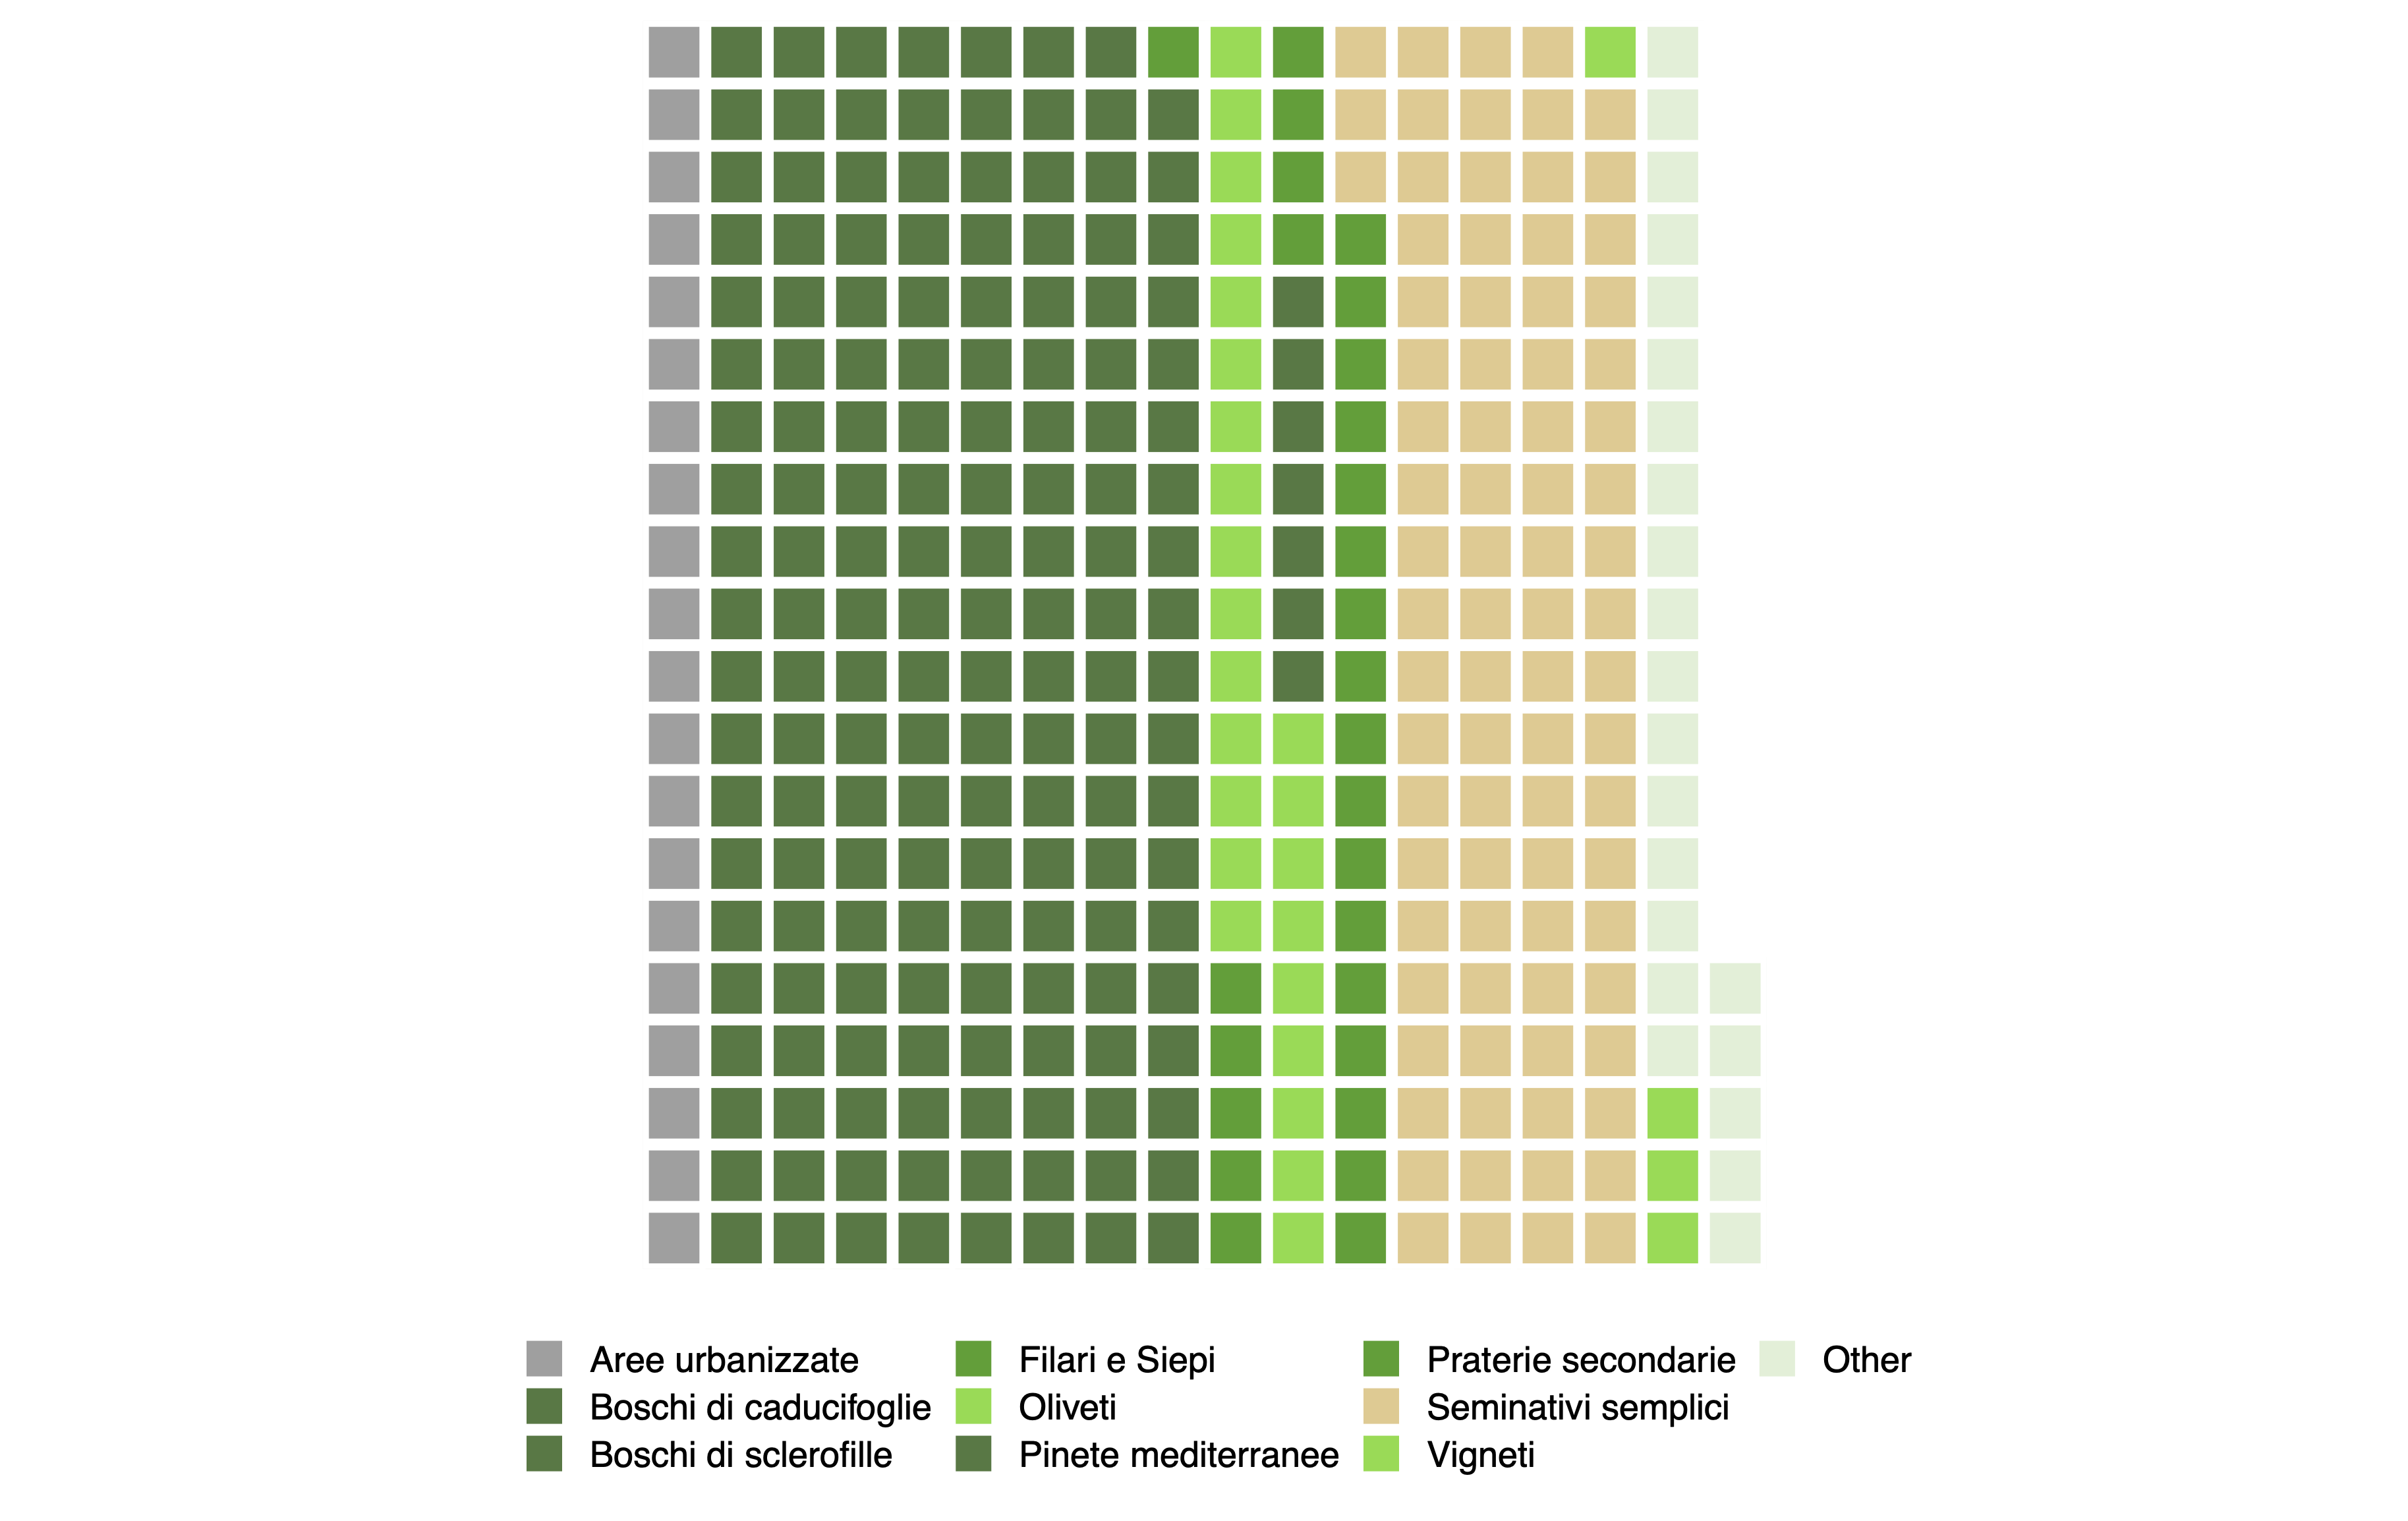
\includegraphics[width=50.75in]{./figs/RECSpoleto_usoSuoloPlot} \caption{Categorie di uso del suolo. Ogni cella rappresenta una superficie di 1 $km^2$.}\label{fig:usoSuolo}
\end{figure}

Esaminando la ripartizione di queste categorie geobotaniche nelle 18 unità di paesaggio, ridotte a 12 attraverso l'aggregazione di tutti gli elementi con configurazione di area urbana, che caratterizzano il territorio spoletino emerge (Fig. \ref{fig:unitaPaes}):

\begin{itemize}
\item
  una \textbf{dominanza forestale nelle aree montane}.
  Infatti, le unità dei castagneti (Montebibico, Vallocchia) e dei pascoli montani (Patrico e Fionchi, Monte Pianciano, Monteluco) mostrano una copertura boschiva predominante, che raggiunge punte dell'88-93\% della superficie;
\item
  una \textbf{vocazione agricola delle aree collinari e di fondovalle}.
  In questo caso l'Unità del Paesaggio della Maroggia e quella dei Sodicci di Poreta presentano un'elevata percentuale di seminativi (rispettivamente 76,7\% e 62,7\%);
\item
  e una \textbf{specializzazione olivicola} nell'Unità degli Oliveti gradonati, che come suggerisce il nome, si caratterizza per la significativa presenza di oliveti e frutteti (42,3\%) combinata con boschi (32,7\%).
\end{itemize}

\begin{figure}

{\centering 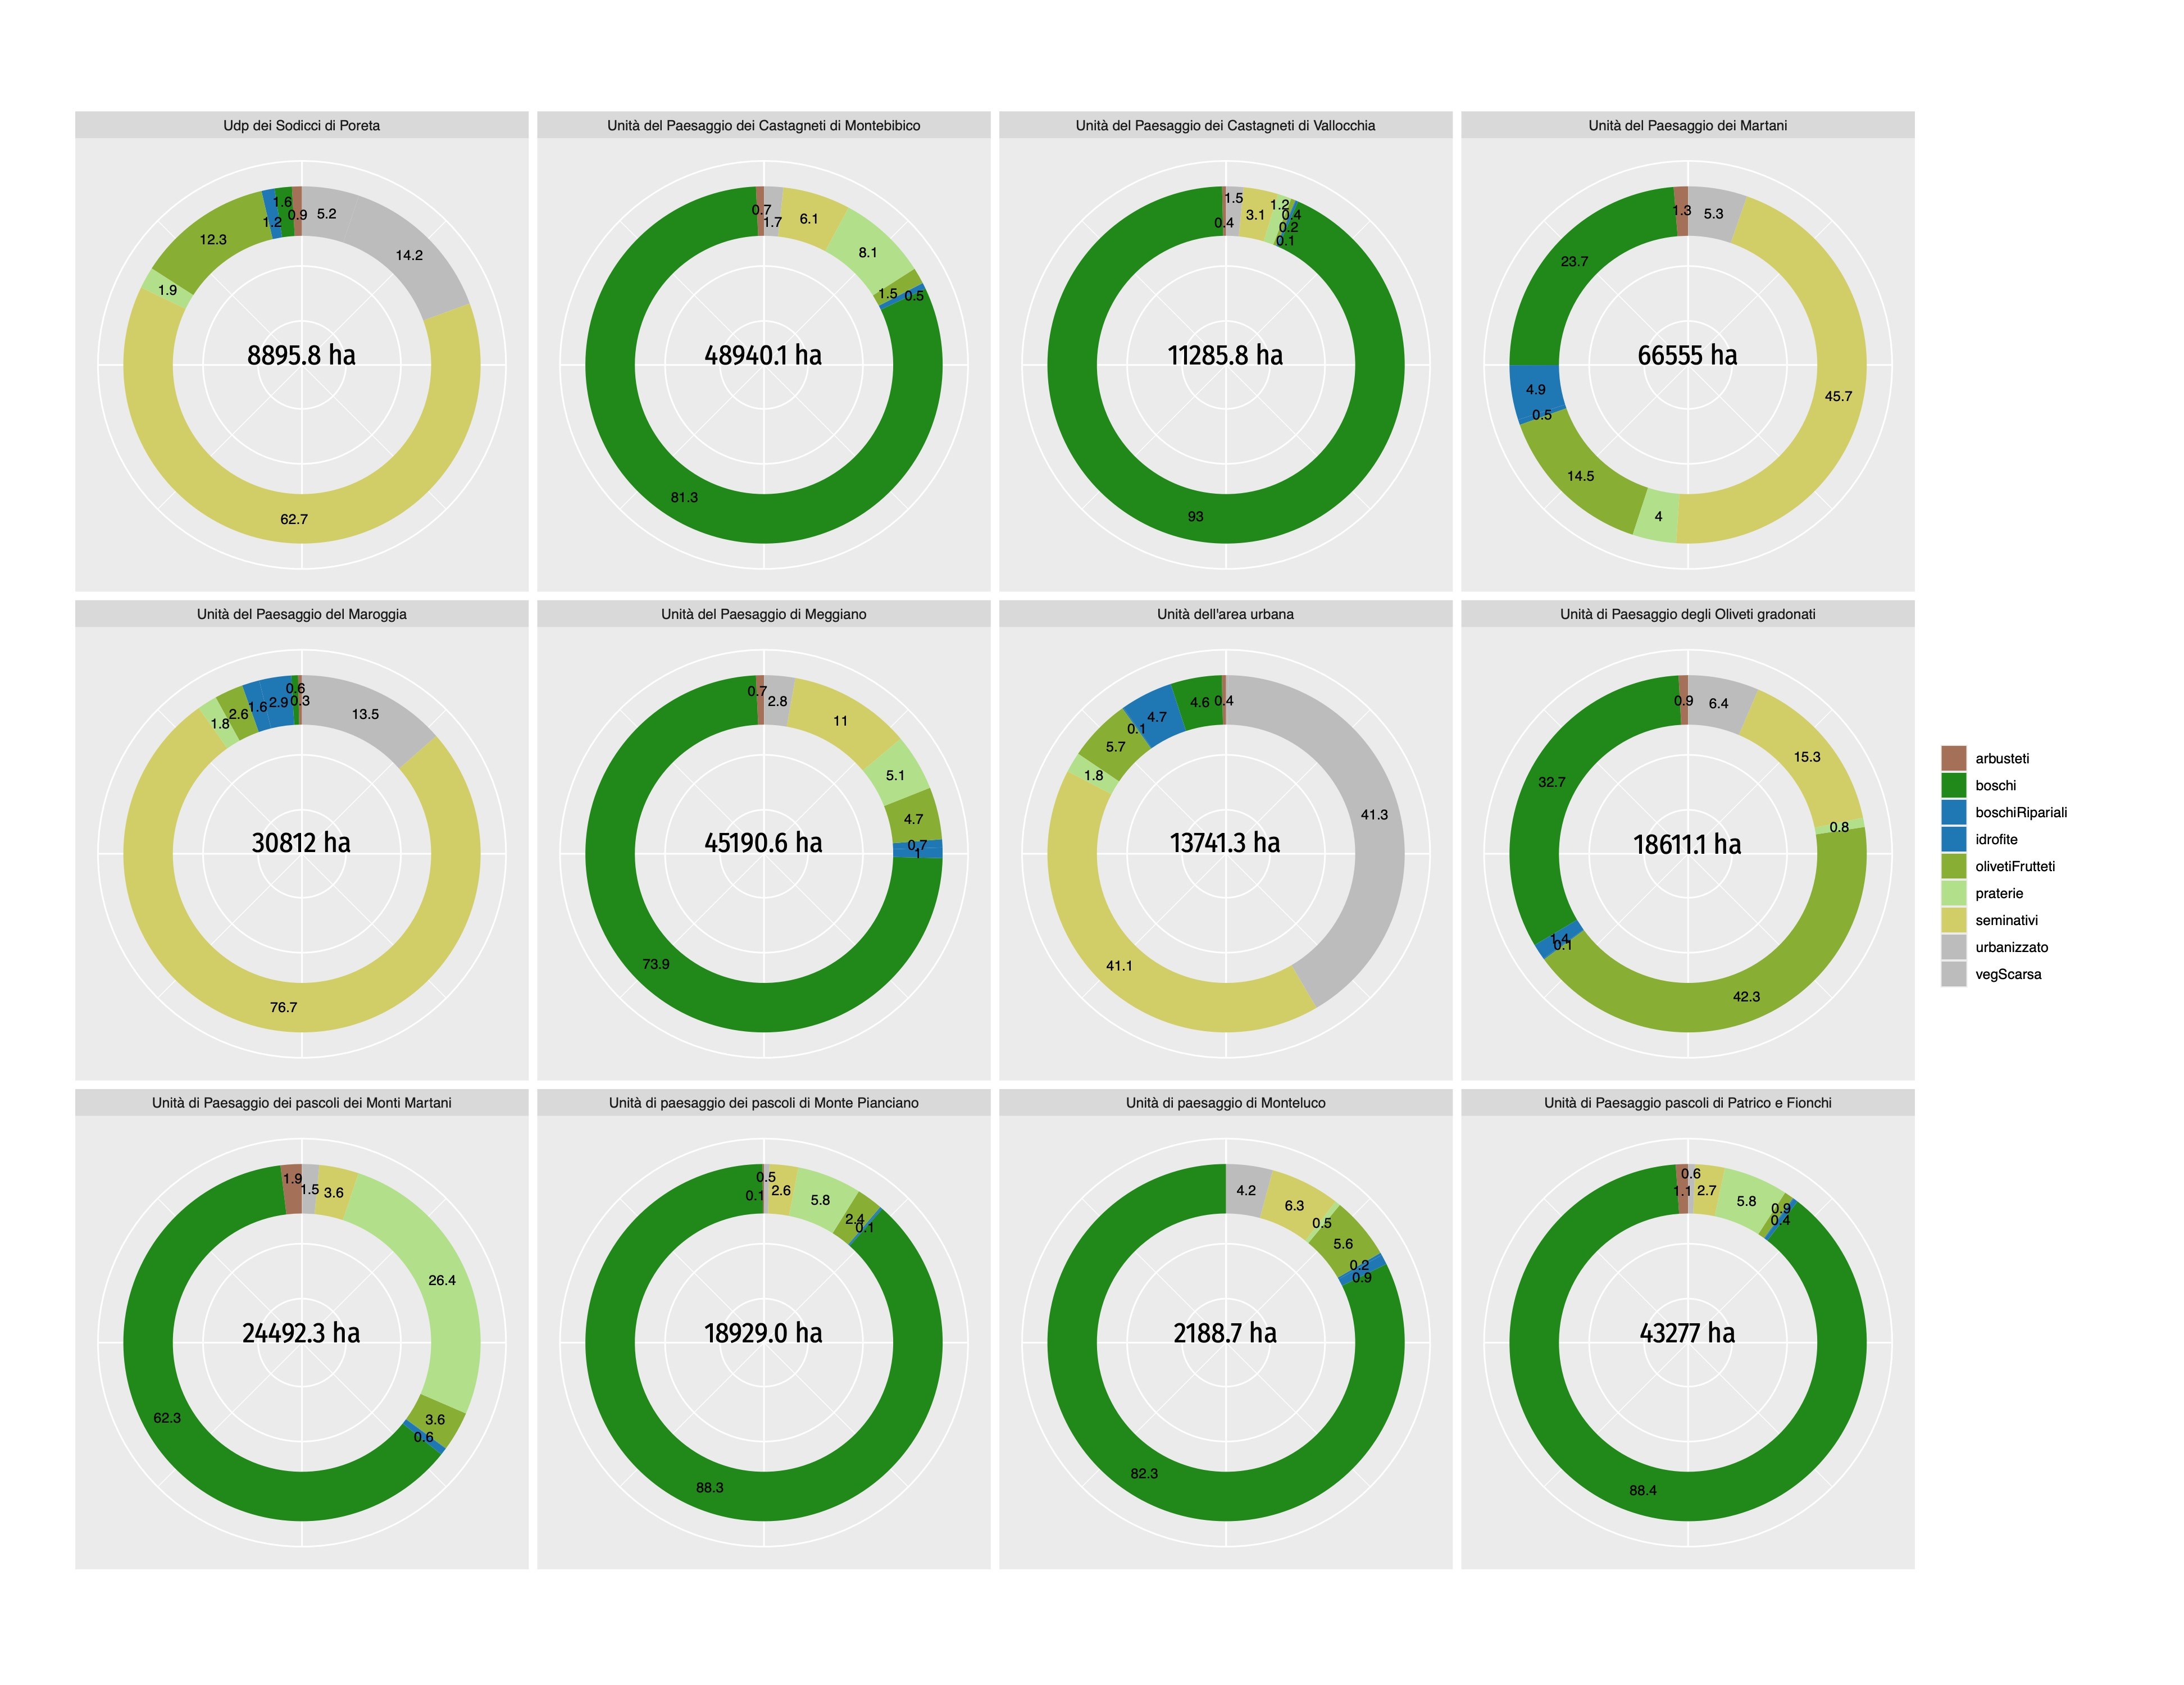
\includegraphics[width=\linewidth]{./figs/RECSpoleto_unitaPaesaggioPlot} 

}

\caption{Tipizzazione degli usi del suolo delle diverse Unità di paesaggio.}\label{fig:unitaPaes}
\end{figure}

Passando invece al calcolo delle metriche e degli indici fragstat relativi ai pattern spaziali per quelle categorie di uso del suolo con una soglia di rappresentanza di almento 1\% emerge il quadro riportato in Tab.
\ref{tab:fragIndex1}.
I dati dell'indice NP (Numero di Patches) descrivono un paesaggio piuttosto diversificato.
Escludendo le tessere del tessuto urbanizzato (5866), le tessere presenti in quantità maggiore sono: filari e siepi (classe 70) 3846 elementi, seminativi semplici (classe 141) 1046 elementi, praterie secondarie submediterranee (classe 91) 1022 elementi e gli oliveti (classe 160) 998 elementi.
Gli indici prodotti da MPA (Tab. \ref{tab:fragIndex1}) e LPI (Tab. \ref{tab:fragIndex2}, Fig. \ref{fig:fragIndex2f}) dimostrano invece che le classi che presentano patches mediamente più grandi sono: le pinete mediterranee (classe 12), i boschi caducifoglie collinare e submontane (classe 22), i boschi di sclerofille mediterranee (classe 11), i boschi di caducifoglie montane (classe 31) e i seminativi semplici (classe 141).
Come atteso, le aree con il numero maggiore di patches sono caratterizzate da tessere di dimensione molto minore, indice di una maggiore frammentazione di queste tipologie territoriali.
La presenza di numerose patches di piccole dimensioni disperse sul territorio, rappresentanti in particolar modo le aree urbane e i seminativi semplici, portano a supportare l'ipotesi di uno sviluppo territoriale antropico in cui si evidenzia un certo sprawl urbano.
Queste indicazioni sono avvalorate anche dai bassi valori restituiti dall'indice di coesione, che presenta un valore medio (±ds) di 9.56±0.365 in una scala compresa tra 0 e 100.

\begin{longtable}[]{@{}
  >{\raggedleft\arraybackslash}p{(\linewidth - 10\tabcolsep) * \real{0.1667}}
  >{\raggedleft\arraybackslash}p{(\linewidth - 10\tabcolsep) * \real{0.1667}}
  >{\raggedleft\arraybackslash}p{(\linewidth - 10\tabcolsep) * \real{0.1667}}
  >{\raggedleft\arraybackslash}p{(\linewidth - 10\tabcolsep) * \real{0.1667}}
  >{\raggedleft\arraybackslash}p{(\linewidth - 10\tabcolsep) * \real{0.1667}}
  >{\raggedleft\arraybackslash}p{(\linewidth - 10\tabcolsep) * \real{0.1667}}@{}}
\caption{\label{tab:fragIndex1} Indici fragstats per l'analisi dei pattern spaziali.}\tabularnewline
\toprule\noalign{}
\begin{minipage}[b]{\linewidth}\raggedleft
Cat. geobot
\end{minipage} & \begin{minipage}[b]{\linewidth}\raggedleft
Number of Patches (NP)
\end{minipage} & \begin{minipage}[b]{\linewidth}\raggedleft
Patch density x 10\^{}6
\end{minipage} & \begin{minipage}[b]{\linewidth}\raggedleft
Mean patch area (MPA)
\end{minipage} & \begin{minipage}[b]{\linewidth}\raggedleft
Median patch area
\end{minipage} & \begin{minipage}[b]{\linewidth}\raggedleft
Edge density (ED)
\end{minipage} \\
\midrule\noalign{}
\endfirsthead
\toprule\noalign{}
\begin{minipage}[b]{\linewidth}\raggedleft
Cat. geobot
\end{minipage} & \begin{minipage}[b]{\linewidth}\raggedleft
Number of Patches (NP)
\end{minipage} & \begin{minipage}[b]{\linewidth}\raggedleft
Patch density x 10\^{}6
\end{minipage} & \begin{minipage}[b]{\linewidth}\raggedleft
Mean patch area (MPA)
\end{minipage} & \begin{minipage}[b]{\linewidth}\raggedleft
Median patch area
\end{minipage} & \begin{minipage}[b]{\linewidth}\raggedleft
Edge density (ED)
\end{minipage} \\
\midrule\noalign{}
\endhead
\bottomrule\noalign{}
\endlastfoot
11 & 104 & 0.298 & 151100.0 & 2400 & 0.0008 \\
12 & 8 & 0.023 & 908650.0 & 144200 & 0.0002 \\
22 & 444 & 1.270 & 325289.6 & 4500 & 0.0061 \\
23 & 55 & 0.157 & 36607.3 & 10300 & 0.0002 \\
31 & 5 & 0.014 & 138220.0 & 11600 & 0.0000 \\
40 & 64 & 0.183 & 30417.2 & 4900 & 0.0003 \\
52 & 5 & 0.014 & 24560.0 & 5400 & 0.0000 \\
61 & 558 & 1.596 & 5265.8 & 2800 & 0.0007 \\
62 & 9 & 0.026 & 18788.9 & 12100 & 0.0000 \\
70 & 3846 & 11.002 & 1362.0 & 700 & 0.0030 \\
91 & 1022 & 2.924 & 22502.6 & 3700 & 0.0027 \\
92 & 16 & 0.046 & 28312.5 & 9050 & 0.0001 \\
93 & 10 & 0.029 & 20570.0 & 10700 & 0.0000 \\
94 & 157 & 0.449 & 9365.0 & 2900 & 0.0003 \\
101 & 95 & 0.272 & 7260.0 & 1200 & 0.0001 \\
102 & 173 & 0.495 & 1772.8 & 400 & 0.0002 \\
111 & 47 & 0.134 & 8970.2 & 900 & 0.0001 \\
120 & 22 & 0.063 & 1877.3 & 1100 & 0.0000 \\
130 & 73 & 0.209 & 32250.7 & 8900 & 0.0002 \\
141 & 1046 & 2.992 & 80969.8 & 7150 & 0.0067 \\
142 & 67 & 0.192 & 9494.0 & 6500 & 0.0001 \\
151 & 248 & 0.709 & 11431.0 & 5550 & 0.0005 \\
152 & 93 & 0.266 & 7332.3 & 5100 & 0.0001 \\
160 & 998 & 2.855 & 24211.8 & 5000 & 0.0028 \\
170 & 343 & 0.981 & 8626.2 & 2500 & 0.0004 \\
180 & 19 & 0.054 & 6821.1 & 3800 & 0.0000 \\
191 & 211 & 0.604 & 13845.0 & 7200 & 0.0004 \\
200 & 5866 & 16.781 & 3504.8 & 300 & 0.0045 \\
210 & 20 & 0.057 & 26045.0 & 4050 & 0.0000 \\
\end{longtable}

\begin{longtable}[]{@{}
  >{\raggedright\arraybackslash}p{(\linewidth - 6\tabcolsep) * \real{0.2500}}
  >{\centering\arraybackslash}p{(\linewidth - 6\tabcolsep) * \real{0.2500}}
  >{\centering\arraybackslash}p{(\linewidth - 6\tabcolsep) * \real{0.2500}}
  >{\centering\arraybackslash}p{(\linewidth - 6\tabcolsep) * \real{0.2500}}@{}}
\caption{\label{tab:fragIndex2} Indici fragstats per l'analisi dei pattern spaziali.}\tabularnewline
\toprule\noalign{}
\begin{minipage}[b]{\linewidth}\raggedright
Class
\end{minipage} & \begin{minipage}[b]{\linewidth}\centering
Largest Patch Index (LPI)
\end{minipage} & \begin{minipage}[b]{\linewidth}\centering
Fractal Dimension Index
\end{minipage} & \begin{minipage}[b]{\linewidth}\centering
Patch cohesion index
\end{minipage} \\
\midrule\noalign{}
\endfirsthead
\toprule\noalign{}
\begin{minipage}[b]{\linewidth}\raggedright
Class
\end{minipage} & \begin{minipage}[b]{\linewidth}\centering
Largest Patch Index (LPI)
\end{minipage} & \begin{minipage}[b]{\linewidth}\centering
Fractal Dimension Index
\end{minipage} & \begin{minipage}[b]{\linewidth}\centering
Patch cohesion index
\end{minipage} \\
\midrule\noalign{}
\endhead
\bottomrule\noalign{}
\endlastfoot
11 & 1.122 & 1.109 & 9.916 \\
12 & 1.229 & 1.134 & 9.937 \\
22 & 31.351 & 1.114 & 9.984 \\
23 & 0.102 & 1.111 & 9.720 \\
31 & 0.178 & 1.120 & 9.860 \\
40 & 0.186 & 1.171 & 9.796 \\
52 & 0.030 & 1.116 & 9.653 \\
61 & 0.037 & 1.106 & 9.224 \\
62 & 0.016 & 1.121 & 9.421 \\
70 & 0.010 & 1.136 & 8.537 \\
91 & 0.865 & 1.113 & 9.874 \\
92 & 0.058 & 1.153 & 9.702 \\
93 & 0.025 & 1.101 & 9.544 \\
94 & 0.049 & 1.119 & 9.542 \\
101 & 0.082 & 1.054 & 9.688 \\
102 & 0.015 & 1.132 & 9.221 \\
111 & 0.049 & 1.141 & 9.676 \\
120 & 0.003 & 1.134 & 8.629 \\
130 & 0.152 & 1.101 & 9.751 \\
141 & 12.789 & 1.108 & 9.971 \\
142 & 0.025 & 1.101 & 9.304 \\
151 & 0.041 & 1.110 & 9.460 \\
152 & 0.012 & 1.109 & 9.163 \\
160 & 1.139 & 1.103 & 9.849 \\
170 & 0.120 & 1.086 & 9.606 \\
180 & 0.012 & 1.088 & 9.210 \\
191 & 0.043 & 1.087 & 9.458 \\
200 & 2.004 & 1.087 & 9.911 \\
210 & 0.052 & 1.082 & 9.689 \\
\end{longtable}

\begin{figure}
\centering
\pandocbounded{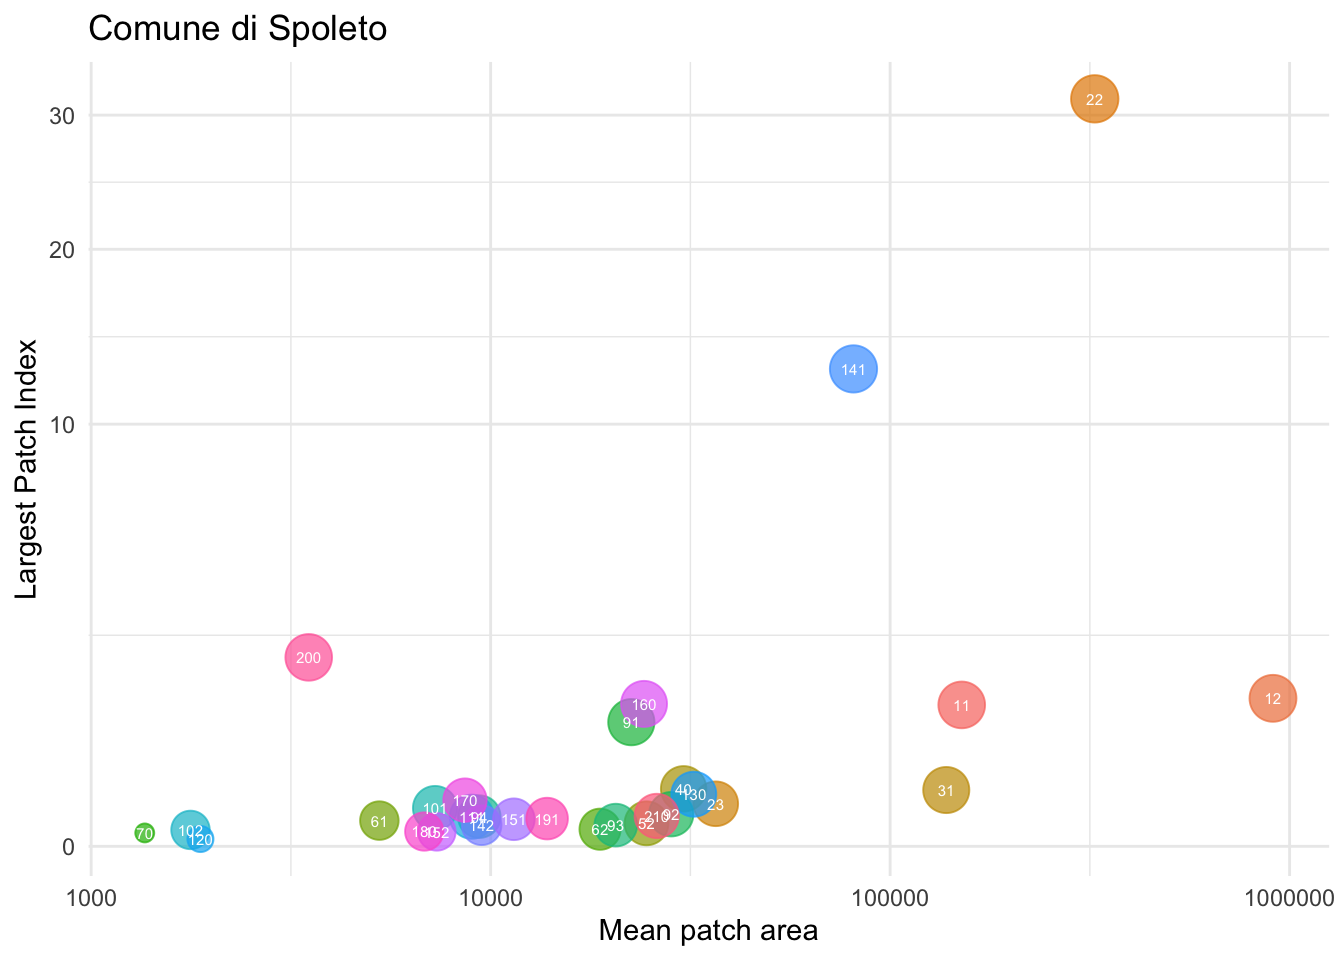
\includegraphics[keepaspectratio]{_main_files/figure-latex/fragIndex2f-1.pdf}}
\caption{\label{fig:fragIndex2f}Plot degli Indici fragstats per Classe geobotanica. Il codice della Classe è riportato all'interno del singolo punto. La dimensione dei punti è proporzionale al valore del Patch cohesion index.}
\end{figure}

Limitando l'analisi alla sola unità di paesaggio urbano, risultante dalla combinazione delle Unità di Paesaggio San Carlo, dei Cappuccini, del Colle S.Elia, del Colle S. Tommaso, di Collerisana e della Valle Urbanizzata, il set di indicatori evidenzia che circa di 76\% del territorio è costituito da Aree urbanizzate (200) e Seminativi semplici (141), mentre se si esclude questa unità e si considerano solo le altre unità di paesaggio il 43\% della superficie è occupata dai boschi di caducifoglie (22) e il 24\% dai seminativi (141).
Tutte le altre categorie presentano una copertura inferiore al 10\%.
La sintesi dei risultati dei pattern spaziali è mostrata nelle tabelle (Tabb. \ref{tab:fragUrbano} e \ref{tab:noUrb}) e nelle figure (Fig. \ref{fig:fragUrbano} e Fig. \ref{fig:fragNoUrb}).

\begin{longtable}[]{@{}
  >{\raggedleft\arraybackslash}p{(\linewidth - 20\tabcolsep) * \real{0.0909}}
  >{\raggedleft\arraybackslash}p{(\linewidth - 20\tabcolsep) * \real{0.0909}}
  >{\raggedleft\arraybackslash}p{(\linewidth - 20\tabcolsep) * \real{0.0909}}
  >{\raggedleft\arraybackslash}p{(\linewidth - 20\tabcolsep) * \real{0.0909}}
  >{\raggedleft\arraybackslash}p{(\linewidth - 20\tabcolsep) * \real{0.0909}}
  >{\raggedleft\arraybackslash}p{(\linewidth - 20\tabcolsep) * \real{0.0909}}
  >{\raggedleft\arraybackslash}p{(\linewidth - 20\tabcolsep) * \real{0.0909}}
  >{\raggedleft\arraybackslash}p{(\linewidth - 20\tabcolsep) * \real{0.0909}}
  >{\raggedleft\arraybackslash}p{(\linewidth - 20\tabcolsep) * \real{0.0909}}
  >{\raggedleft\arraybackslash}p{(\linewidth - 20\tabcolsep) * \real{0.0909}}
  >{\raggedleft\arraybackslash}p{(\linewidth - 20\tabcolsep) * \real{0.0909}}@{}}
\caption{\label{tab:fragUrbano} Indici fragstats per l'analisi dei pattern spaziali per l'unità di paesaggio urbano.}\tabularnewline
\toprule\noalign{}
\begin{minipage}[b]{\linewidth}\raggedleft
Cat. geobot
\end{minipage} & \begin{minipage}[b]{\linewidth}\raggedleft
Land cover
\end{minipage} & \begin{minipage}[b]{\linewidth}\raggedleft
Landscape Proportion
\end{minipage} & \begin{minipage}[b]{\linewidth}\raggedleft
Edge length
\end{minipage} & \begin{minipage}[b]{\linewidth}\raggedleft
Edge density
\end{minipage} & \begin{minipage}[b]{\linewidth}\raggedleft
Number of Patches
\end{minipage} & \begin{minipage}[b]{\linewidth}\raggedleft
Patch density
\end{minipage} & \begin{minipage}[b]{\linewidth}\raggedleft
Greatest patch area
\end{minipage} & \begin{minipage}[b]{\linewidth}\raggedleft
Smallest patch area
\end{minipage} & \begin{minipage}[b]{\linewidth}\raggedleft
Mean patch area
\end{minipage} & \begin{minipage}[b]{\linewidth}\raggedleft
Median patch area
\end{minipage} \\
\midrule\noalign{}
\endfirsthead
\toprule\noalign{}
\begin{minipage}[b]{\linewidth}\raggedleft
Cat. geobot
\end{minipage} & \begin{minipage}[b]{\linewidth}\raggedleft
Land cover
\end{minipage} & \begin{minipage}[b]{\linewidth}\raggedleft
Landscape Proportion
\end{minipage} & \begin{minipage}[b]{\linewidth}\raggedleft
Edge length
\end{minipage} & \begin{minipage}[b]{\linewidth}\raggedleft
Edge density
\end{minipage} & \begin{minipage}[b]{\linewidth}\raggedleft
Number of Patches
\end{minipage} & \begin{minipage}[b]{\linewidth}\raggedleft
Patch density
\end{minipage} & \begin{minipage}[b]{\linewidth}\raggedleft
Greatest patch area
\end{minipage} & \begin{minipage}[b]{\linewidth}\raggedleft
Smallest patch area
\end{minipage} & \begin{minipage}[b]{\linewidth}\raggedleft
Mean patch area
\end{minipage} & \begin{minipage}[b]{\linewidth}\raggedleft
Median patch area
\end{minipage} \\
\midrule\noalign{}
\endhead
\bottomrule\noalign{}
\endlastfoot
11 & 100400 & 0.01 & 4140 & 0.00 & 2 & 0 & 100300 & 100 & 50200.00 & 50200 \\
22 & 564700 & 0.04 & 38400 & 0.00 & 36 & 0 & 315700 & 100 & 15686.11 & 5200 \\
40 & 7300 & 0.00 & 980 & 0.00 & 4 & 0 & 4900 & 100 & 1825.00 & 1150 \\
61 & 24100 & 0.00 & 2220 & 0.00 & 6 & 0 & 11600 & 300 & 4016.67 & 2400 \\
70 & 724500 & 0.05 & 141720 & 0.01 & 482 & 0 & 35200 & 100 & 1503.11 & 700 \\
91 & 265000 & 0.02 & 18860 & 0.00 & 36 & 0 & 77100 & 100 & 7361.11 & 150 \\
101 & 3200 & 0.00 & 440 & 0.00 & 2 & 0 & 2600 & 600 & 1600.00 & 1600 \\
102 & 3900 & 0.00 & 820 & 0.00 & 3 & 0 & 3300 & 100 & 1300.00 & 500 \\
111 & 6000 & 0.00 & 1240 & 0.00 & 9 & 0 & 3600 & 100 & 666.67 & 200 \\
141 & 5648700 & 0.38 & 204480 & 0.01 & 85 & 0 & 2876200 & 100 & 66455.29 & 3000 \\
142 & 44400 & 0.00 & 3480 & 0.00 & 7 & 0 & 17400 & 700 & 6342.86 & 4700 \\
151 & 234600 & 0.02 & 19480 & 0.00 & 36 & 0 & 73200 & 800 & 6516.67 & 4150 \\
152 & 123600 & 0.01 & 9140 & 0.00 & 19 & 0 & 22600 & 100 & 6505.26 & 5600 \\
160 & 1032500 & 0.07 & 67480 & 0.00 & 119 & 0 & 218700 & 100 & 8676.47 & 2500 \\
170 & 93000 & 0.01 & 10400 & 0.00 & 37 & 0 & 10400 & 600 & 2513.51 & 1900 \\
180 & 3300 & 0.00 & 360 & 0.00 & 1 & 0 & 3300 & 3300 & 3300.00 & 3300 \\
191 & 270900 & 0.02 & 12940 & 0.00 & 18 & 0 & 101200 & 100 & 15050.00 & 4450 \\
200 & 5667200 & 0.38 & 199060 & 0.01 & 312 & 0 & 4787700 & 100 & 18164.10 & 700 \\
210 & 21000 & 0.00 & 720 & 0.00 & 1 & 0 & 21000 & 21000 & 21000.00 & 21000 \\
\end{longtable}

\begin{longtable}[]{@{}
  >{\raggedleft\arraybackslash}p{(\linewidth - 20\tabcolsep) * \real{0.0909}}
  >{\raggedleft\arraybackslash}p{(\linewidth - 20\tabcolsep) * \real{0.0909}}
  >{\raggedleft\arraybackslash}p{(\linewidth - 20\tabcolsep) * \real{0.0909}}
  >{\raggedleft\arraybackslash}p{(\linewidth - 20\tabcolsep) * \real{0.0909}}
  >{\raggedleft\arraybackslash}p{(\linewidth - 20\tabcolsep) * \real{0.0909}}
  >{\raggedleft\arraybackslash}p{(\linewidth - 20\tabcolsep) * \real{0.0909}}
  >{\raggedleft\arraybackslash}p{(\linewidth - 20\tabcolsep) * \real{0.0909}}
  >{\raggedleft\arraybackslash}p{(\linewidth - 20\tabcolsep) * \real{0.0909}}
  >{\raggedleft\arraybackslash}p{(\linewidth - 20\tabcolsep) * \real{0.0909}}
  >{\raggedleft\arraybackslash}p{(\linewidth - 20\tabcolsep) * \real{0.0909}}
  >{\raggedleft\arraybackslash}p{(\linewidth - 20\tabcolsep) * \real{0.0909}}@{}}
\caption{\label{tab:noUrb} Indici fragstats per l'analisi dei pattern spaziali per tutte le unità di paesaggio ad esclusione di quella urbana.}\tabularnewline
\toprule\noalign{}
\begin{minipage}[b]{\linewidth}\raggedleft
Cat. geobot
\end{minipage} & \begin{minipage}[b]{\linewidth}\raggedleft
Land cover
\end{minipage} & \begin{minipage}[b]{\linewidth}\raggedleft
Landscape Proportion
\end{minipage} & \begin{minipage}[b]{\linewidth}\raggedleft
Edge length
\end{minipage} & \begin{minipage}[b]{\linewidth}\raggedleft
Edge.density
\end{minipage} & \begin{minipage}[b]{\linewidth}\raggedleft
Number of Patches
\end{minipage} & \begin{minipage}[b]{\linewidth}\raggedleft
Patch density x 10\^{}6
\end{minipage} & \begin{minipage}[b]{\linewidth}\raggedleft
Greatest patch area
\end{minipage} & \begin{minipage}[b]{\linewidth}\raggedleft
Smallest patch area
\end{minipage} & \begin{minipage}[b]{\linewidth}\raggedleft
Mean patch area
\end{minipage} & \begin{minipage}[b]{\linewidth}\raggedleft
Median patch area
\end{minipage} \\
\midrule\noalign{}
\endfirsthead
\toprule\noalign{}
\begin{minipage}[b]{\linewidth}\raggedleft
Cat. geobot
\end{minipage} & \begin{minipage}[b]{\linewidth}\raggedleft
Land cover
\end{minipage} & \begin{minipage}[b]{\linewidth}\raggedleft
Landscape Proportion
\end{minipage} & \begin{minipage}[b]{\linewidth}\raggedleft
Edge length
\end{minipage} & \begin{minipage}[b]{\linewidth}\raggedleft
Edge.density
\end{minipage} & \begin{minipage}[b]{\linewidth}\raggedleft
Number of Patches
\end{minipage} & \begin{minipage}[b]{\linewidth}\raggedleft
Patch density x 10\^{}6
\end{minipage} & \begin{minipage}[b]{\linewidth}\raggedleft
Greatest patch area
\end{minipage} & \begin{minipage}[b]{\linewidth}\raggedleft
Smallest patch area
\end{minipage} & \begin{minipage}[b]{\linewidth}\raggedleft
Mean patch area
\end{minipage} & \begin{minipage}[b]{\linewidth}\raggedleft
Median patch area
\end{minipage} \\
\midrule\noalign{}
\endhead
\bottomrule\noalign{}
\endlastfoot
11 & 15598000 & 0.047 & 277700 & 0.001 & 108 & 0.323 & 3821900 & 100 & 144425.9 & 1900 \\
12 & 7269200 & 0.022 & 77000 & 0.000 & 8 & 0.024 & 4297000 & 600 & 908650.0 & 144200 \\
22 & 143863200 & 0.430 & 2102620 & 0.006 & 424 & 1.267 & 109531200 & 100 & 339300.0 & 4200 \\
23 & 2013400 & 0.006 & 70400 & 0.000 & 55 & 0.164 & 355100 & 500 & 36607.3 & 10300 \\
31 & 691100 & 0.002 & 9640 & 0.000 & 5 & 0.015 & 621900 & 8200 & 138220.0 & 11600 \\
40 & 1939400 & 0.006 & 117080 & 0.000 & 65 & 0.194 & 649100 & 100 & 29836.9 & 4500 \\
52 & 122800 & 0.000 & 3900 & 0.000 & 5 & 0.015 & 104000 & 2800 & 24560.0 & 5400 \\
61 & 2914200 & 0.009 & 238000 & 0.001 & 552 & 1.649 & 129900 & 100 & 5279.3 & 2800 \\
62 & 169100 & 0.001 & 9080 & 0.000 & 9 & 0.027 & 57500 & 3400 & 18788.9 & 12100 \\
70 & 4513700 & 0.013 & 899740 & 0.003 & 3405 & 10.173 & 28200 & 100 & 1325.6 & 600 \\
91 & 22732700 & 0.068 & 940880 & 0.003 & 1014 & 3.029 & 3024500 & 100 & 22418.8 & 3700 \\
92 & 453000 & 0.001 & 19180 & 0.000 & 16 & 0.048 & 202600 & 200 & 28312.5 & 9050 \\
93 & 205700 & 0.001 & 8120 & 0.000 & 10 & 0.030 & 88400 & 800 & 20570.0 & 10700 \\
94 & 1470300 & 0.004 & 95160 & 0.000 & 157 & 0.469 & 173000 & 100 & 9365.0 & 2900 \\
101 & 686500 & 0.002 & 30340 & 0.000 & 93 & 0.278 & 287000 & 100 & 7381.7 & 1200 \\
102 & 302800 & 0.001 & 57480 & 0.000 & 172 & 0.514 & 52800 & 100 & 1760.5 & 400 \\
111 & 415600 & 0.001 & 30600 & 0.000 & 47 & 0.140 & 171900 & 100 & 8842.6 & 900 \\
120 & 41300 & 0.000 & 6000 & 0.000 & 22 & 0.066 & 10500 & 100 & 1877.3 & 1100 \\
130 & 2354300 & 0.007 & 74160 & 0.000 & 73 & 0.218 & 532700 & 100 & 32250.7 & 8900 \\
141 & 79045200 & 0.236 & 2141100 & 0.006 & 1010 & 3.017 & 44707200 & 100 & 78262.6 & 7100 \\
142 & 591700 & 0.002 & 36220 & 0.000 & 61 & 0.182 & 87200 & 100 & 9700.0 & 6500 \\
151 & 2600000 & 0.008 & 149720 & 0.000 & 212 & 0.633 & 143700 & 100 & 12264.2 & 6000 \\
152 & 558300 & 0.002 & 40340 & 0.000 & 80 & 0.239 & 41300 & 200 & 6978.8 & 4200 \\
160 & 23130900 & 0.069 & 905100 & 0.003 & 900 & 2.689 & 3980100 & 100 & 25701.0 & 5400 \\
170 & 2865800 & 0.009 & 141200 & 0.000 & 308 & 0.920 & 418900 & 100 & 9304.5 & 2750 \\
180 & 126300 & 0.000 & 8100 & 0.000 & 18 & 0.054 & 43100 & 1700 & 7016.7 & 4000 \\
191 & 2650400 & 0.008 & 124940 & 0.000 & 197 & 0.589 & 151000 & 100 & 13453.8 & 7500 \\
200 & 14891500 & 0.044 & 1387840 & 0.004 & 5622 & 16.796 & 1905100 & 100 & 2648.8 & 300 \\
210 & 499900 & 0.001 & 14560 & 0.000 & 19 & 0.057 & 181200 & 100 & 26310.5 & 3800 \\
\end{longtable}

\begin{figure}
\centering
\pandocbounded{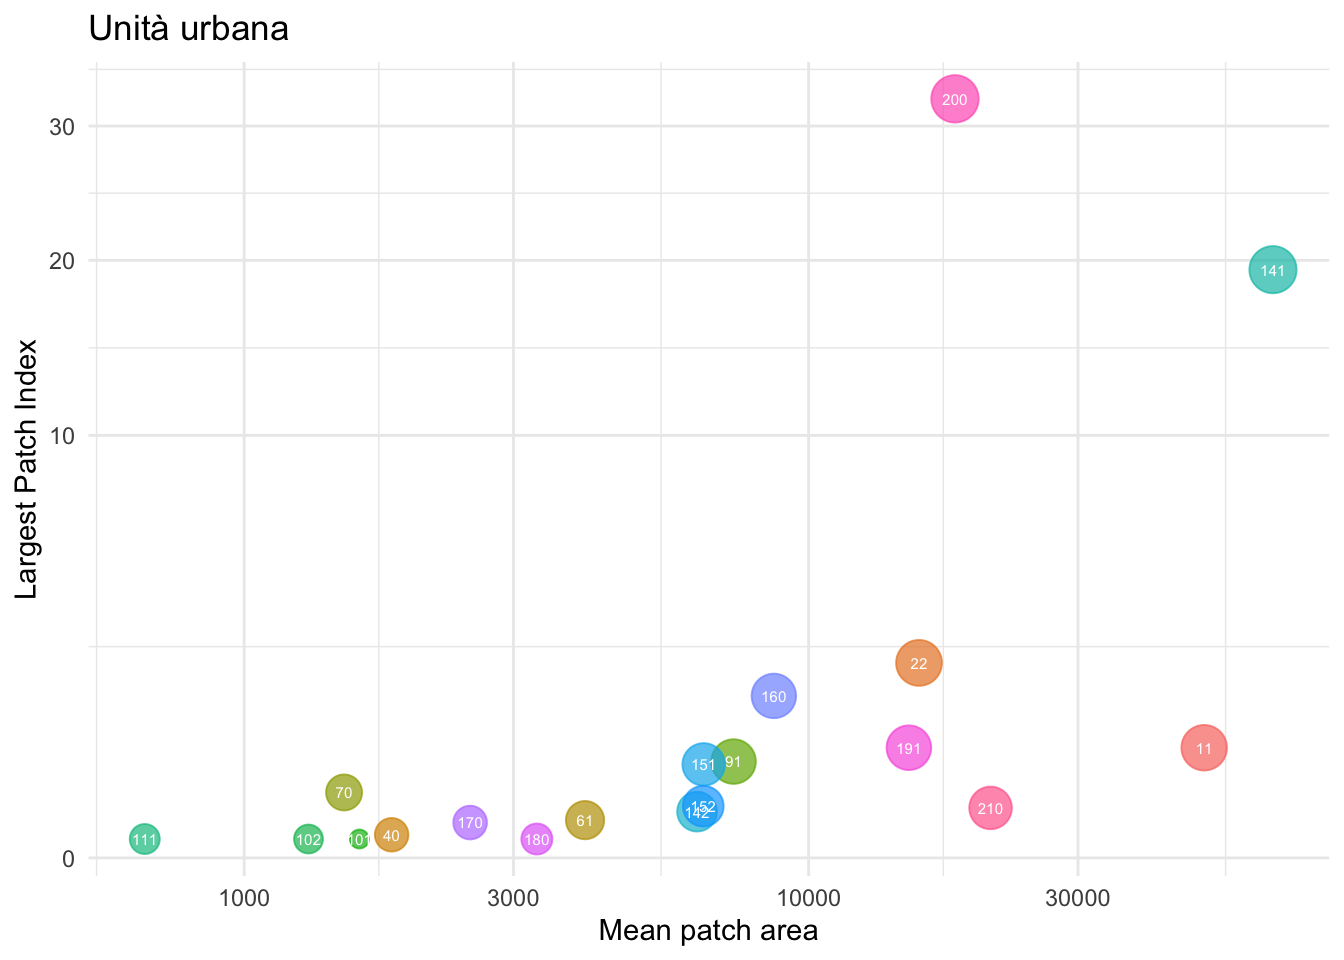
\includegraphics[keepaspectratio]{_main_files/figure-latex/fragUrbano-1.pdf}}
\caption{\label{fig:fragUrbano}Plot degli Indici fragstats per Classe geobotanica in Unità urbana. Il codice della Classe è riportato all'interno del singolo punto. La dimensione dei punti è proporzionale al valore del Patch cohesion index.}
\end{figure}

\begin{figure}
\centering
\pandocbounded{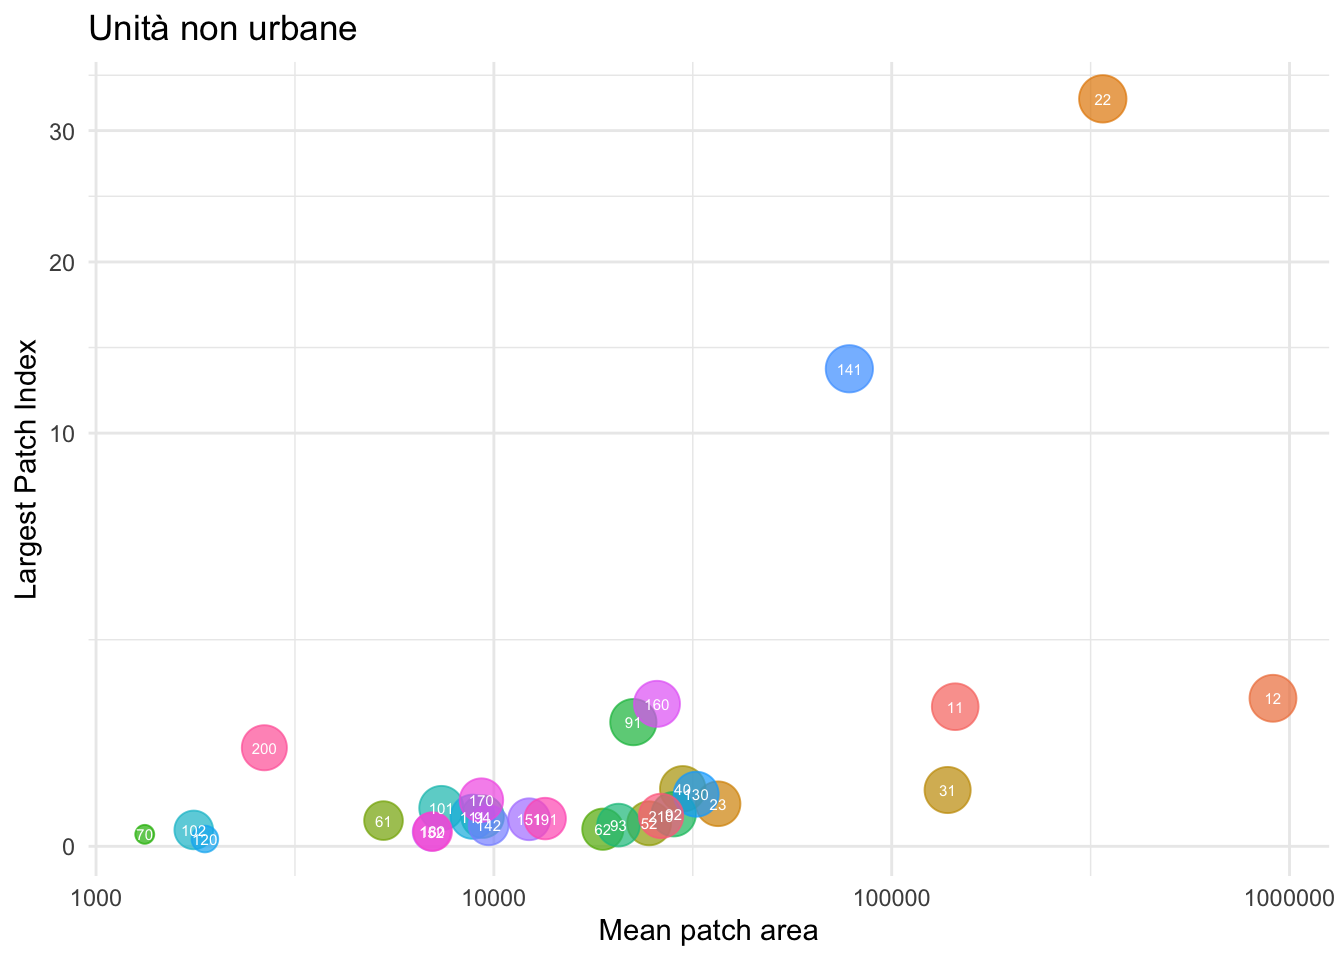
\includegraphics[keepaspectratio]{_main_files/figure-latex/fragNoUrb-1.pdf}}
\caption{\label{fig:fragNoUrb}Plot degli Indici fragstats per Classe geobotanica nell'area non urbana. Il codice della Classe è riportato all'interno del singolo punto. La dimensione dei punti è proporzionale al valore del Patch cohesion index.}
\end{figure}

Riassumendo gli indici di frammentazione del paesaggio e confrontando l'ambiente urbano (U) e quello non urbano (N), emergono alcuni particolari pattern (Tab. \ref{tab:fragComp}).
Come atteso, la maggior parte delle classi di uso del suolo mostra valori di Splitting Index più elevati in ambiente urbano, indicando una frammentazione significativamente maggiore.
Questo si traduce in valori di Effective Meshsize (dimensione effettiva delle patch) sistematicamente più bassi nell'area urbana (particolare attenzione andrebbe riservata alla situazione che emerge per le aree umide in associazione con la Vegetazione idrofitica).
Curiosamente ci sono anche delle eccezioni.
Ad esempio la categoria di Filari e siepi (70) presenta un valore di Splitting Index più alto in ambiente non urbano (N) (5 milioni vs 50.000), suggerendo che in città (U) questi elementi apparentemente sono meno frammentati.
Il valore di Landscape Division rimane costante per quasi tutte le classi in entrambi gli ambienti, indicando che la differenza principale sta nell'intensità della frammentazione piuttosto che nella presenza/assenza delle classi di uso del suolo.

\begin{longtable}[]{@{}
  >{\raggedleft\arraybackslash}p{(\linewidth - 8\tabcolsep) * \real{0.2000}}
  >{\raggedright\arraybackslash}p{(\linewidth - 8\tabcolsep) * \real{0.2000}}
  >{\raggedright\arraybackslash}p{(\linewidth - 8\tabcolsep) * \real{0.2000}}
  >{\raggedright\arraybackslash}p{(\linewidth - 8\tabcolsep) * \real{0.2000}}
  >{\raggedright\arraybackslash}p{(\linewidth - 8\tabcolsep) * \real{0.2000}}@{}}
\caption{\label{tab:fragComp} Confronto tra gli indici fragstats per l'analisi della frammentazione dell'unità di paesaggio urbano (U) rispetto a tutti gli altri (N).}\tabularnewline
\toprule\noalign{}
\begin{minipage}[b]{\linewidth}\raggedleft
Cat
\end{minipage} & \begin{minipage}[b]{\linewidth}\raggedright
geobot
\end{minipage} & \begin{minipage}[b]{\linewidth}\raggedright
Landscape division U/N
\end{minipage} & \begin{minipage}[b]{\linewidth}\raggedright
Splitting Index U/N
\end{minipage} & \begin{minipage}[b]{\linewidth}\raggedright
Effective Meshsize U/N
\end{minipage} \\
\midrule\noalign{}
\endfirsthead
\toprule\noalign{}
\begin{minipage}[b]{\linewidth}\raggedleft
Cat
\end{minipage} & \begin{minipage}[b]{\linewidth}\raggedright
geobot
\end{minipage} & \begin{minipage}[b]{\linewidth}\raggedright
Landscape division U/N
\end{minipage} & \begin{minipage}[b]{\linewidth}\raggedright
Splitting Index U/N
\end{minipage} & \begin{minipage}[b]{\linewidth}\raggedright
Effective Meshsize U/N
\end{minipage} \\
\midrule\noalign{}
\endhead
\bottomrule\noalign{}
\endlastfoot
11 & Boschi di sclerofille mediterranee & 1.00 / 1.000 & 21886 / 3983 & 678 / 84042 \\
22 & Boschi caducifoglie collinari/submontane & 1.00 / 0.890 & 2135 / 9.111 & 6950 / 36737401 \\
40 & Boschi ripariali & 1.00 / 1.000 & 7626434 / 191315 & 1.95 / 1750 \\
61 & Arbusteti collinari & 1.00 / 1.000 & 1201108 / 1757651 & 12.35 / 190.43 \\
70 & Filari e siepi & 1.00 / 1.000 & 50367 / 5058464 & 295 / 66 \\
91 & Praterie secondarie submediterranee & 1.00 / 1.000 & 14954 / 5094 & 992 / 65708 \\
101 & Vegetazione idrofitica lacustre & 1.00 / 1.000 & 30923476 / 1189363 & 0.48 / 281.43 \\
102 & Vegetazione idrofitica fluviale & 1.00 / 1.000 & 19746650 / 22762551 & 0.75 / 14.71 \\
111 & Popolamenti terofitici & 1.00 / 1.000 & 15440052 / 2673476 & 0.96 / 125.20 \\
141 & Seminativi semplici & 0.96 / 0.982 & 23.15 / 55.25 & 640915 / 6057904 \\
142 & Campi abbandonati e incolti & 1.00 / 1.000 & 471790 / 7286123 & 31.45 / 45.94 \\
151 & Seminativi arborati & 1.00 / 1.000 & 34825 / 986556 & 426 / 339 \\
152 & Colture agrarie mosaicizzate & 1.00 / 1.000 & 136995 / 12101779 & 108 / 28 \\
160 & Oliveti & 1.00 / 1.000 & 3171 / 5472 & 4680 / 61173 \\
170 & Vigneti & 1.00 / 1.000 & 561356 / 394606 & 26.43 / 848.23 \\
180 & Frutteti & 1.00 / 1.000 & 20218103 / 45930479 & 0.73 / 7.29 \\
191 & Arboricoltura da legno & 1.00 / 1.000 & 13532 / 1096137 & 1097 / 305 \\
200 & Aree urbanizzate & 0.90 / 1.000 & 9.59 / 22584 & 1546716 / 14821 \\
210 & Vegetazione scarsa o nulla & 1.00 / 1.000 & 499263 / 1875870 & 29.72 / 178.43 \\
\end{longtable}

\subsection{Carte di idoneità e della biopermeabilità}\label{carte-di-idoneituxe0-e-della-biopermeabilituxe0}

La disponibilità di una carta geobotanica e di uso del suolo aggiornata rappresenta uno strumento fondamentale per lo sviluppo di analisi ecologiche successive anche in funzione della distribuzione reale e potenziale della fauna.
Infatti tra le principali carte che possono essere derivate da questa cartografia ci sono le carte di idoneità o vocazionalità faunistica e di permeabilità del territorio.
In linea generale, la vocazionalità faunistica di un territorio dipende dalla capacità degli habitat di soddisfare i requisiti ecologici delle diverse specie animali.

Ogni categoria geobotanica presenta caratteristiche specifiche in termini di:

\begin{itemize}
\item
  \textbf{Disponibilità trofica}: diversi tipi di vegetazione offrono risorse alimentari differenziate anche in funzione dei loro cicli vegetativi;
\item
  \textbf{Struttura dell'habitat}: la complessità verticale e orizzontale della vegetazione influenza le possibilità di rifugio e possibilità per la riproduzione;
\item
  \textbf{Condizioni microclimatiche}: i diversi tipi di copertura vegetale creano condizioni ambientali specifiche in relazione a temperatura, esposizione e umidità, che possono esssere determinanti per la presenza e l'abbondanza delle specie animali.
\end{itemize}

A titolo di esempio sono state elaborate due carte di sintesi che esprimono una vocazionalità in funzione delle specie con una elezione per gli ambienti forestali (Fig. \ref{fig:cidon}) e che trovano negli elementi di connettività ecologica e struttura del bosco e delle praterie le condizioni di preferenza per il loro habitat e le loro funzioni vitali (Fig. \ref{fig:cbioperm}).

\begin{figure}

{\centering 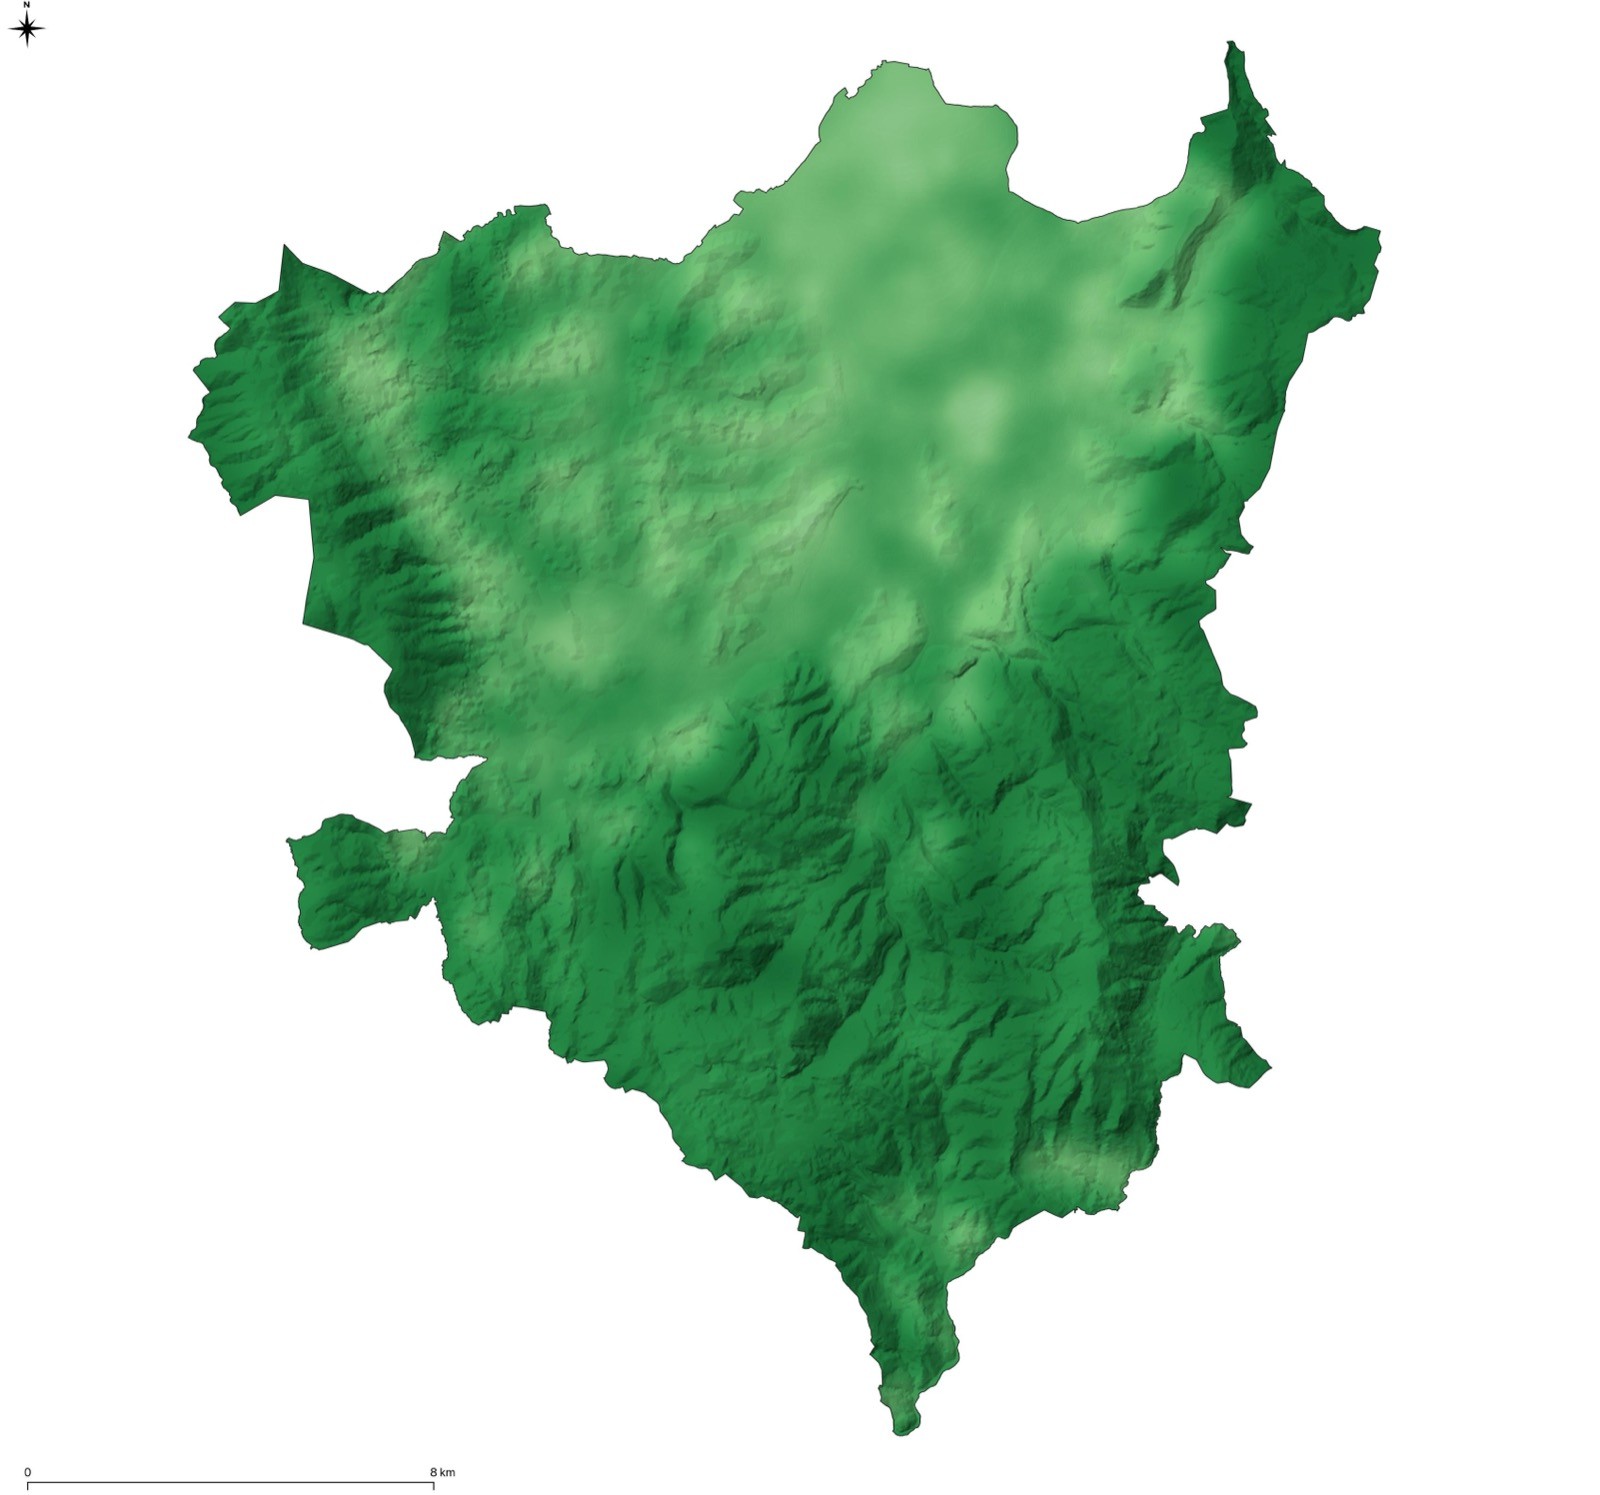
\includegraphics[width=1\linewidth]{./figs/cartaIdoneita} 

}

\caption{Esempio di carta della vocazionalità faunistica sviluppata su un panel di specie con preferenza per habitat forestali.}\label{fig:cidon}
\end{figure}

\begin{figure}

{\centering 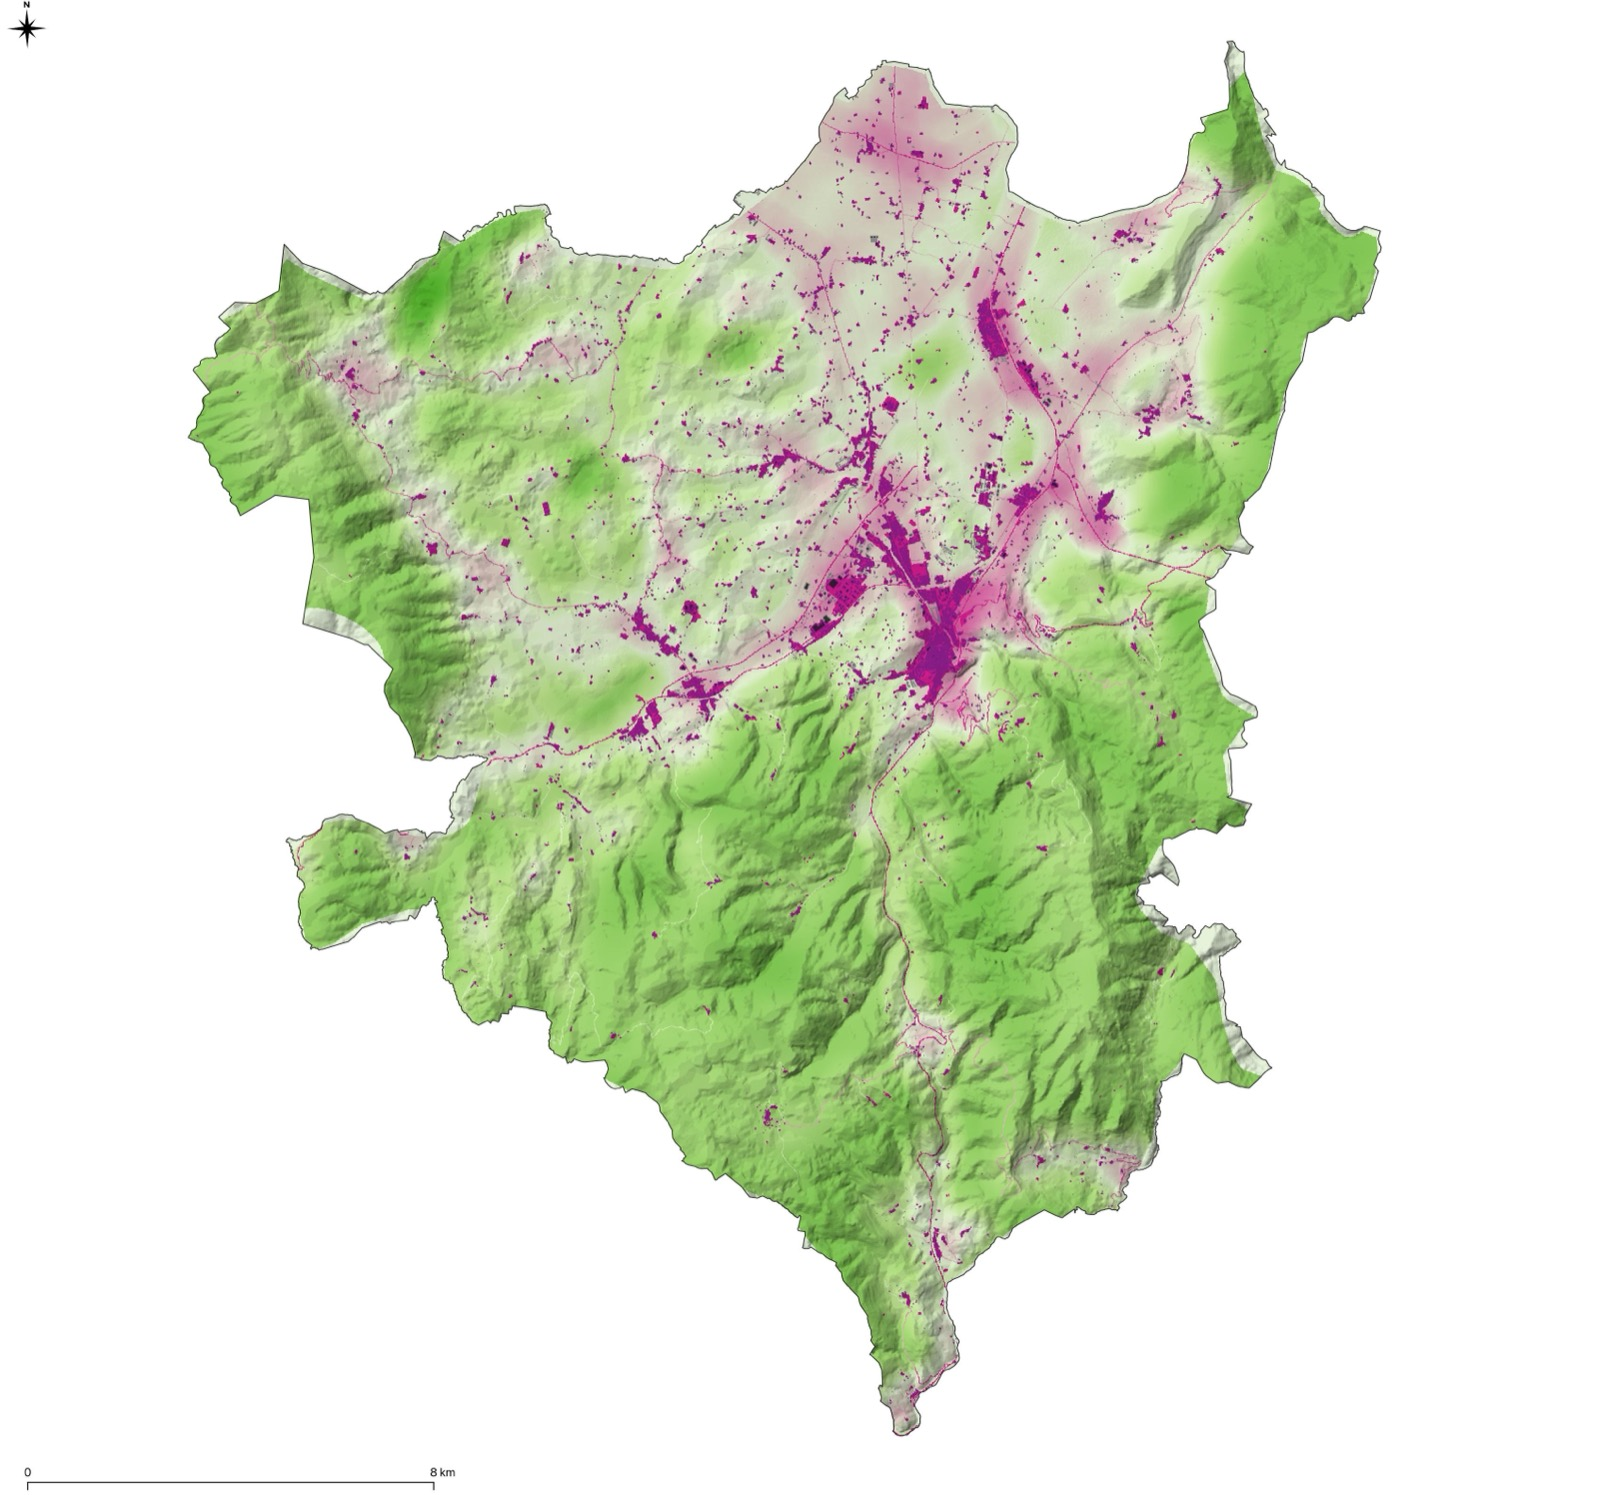
\includegraphics[width=1\linewidth]{./figs/cartaBioperm} 

}

\caption{Esempio di carta della permeabilità tenuto conto dell'idoneità faunistica forestale e della presenza nel territori di elementi di permeabilità (es. corridoi fluviali) e di elementi di frammentazione (es. strade).}\label{fig:cbioperm}
\end{figure}

Successive metodologie di analisi, come ad esempio la \textbf{Cost-distance analysis} (==BIB==) che consiste nel calcolo dei percorsi di minor costo per il movimento delle specie attraverso la matrice paesaggistica, attribuendo diversi valori di resistenza alle categorie di uso del suolo o della \textbf{Graph theory} (==BIB==) che si occupa della modellazione del paesaggio come rete di nodi (habitat favorevoli) connessi da corridoi di diversa permeabilità, potranno suggerire strategie differenziate di gestione territoriale, per il panel di specie che verranno considerate come target specifico e di maggiore interesse ai fini di un approfondimento scientifico-gestionale.
Per alcune specie ombrello, l'analisi potrà evidenziare la necessità di mantenere corridoi su scala comunale tra le diverse unità paesaggistiche.
Per le specie focali (indicatrici della qualità di ecosistemi specifici), si potranno identificare le aree core da preservare e le zone di buffer da associare.
Infine, per le specie bandiera (di particolare valore conservazionistico), l'analisi supporterà la progettazione di interventi mirati al mantenimento o al ripristino ambientale, anche attraverso la creazione di ulteriori elementi di stepping stones, funzionali alla riduzione della frammentazione del territorio e al potenziamento della connettività.

\subsection{Analisi della frammentazione}\label{analisi-della-frammentazione-1}

Per approfondire la valutazione della continuità ecologica e del grado di frammentazione del territorio sono stati applicati tre indici specifici che misurano diversi aspetti della frammentazione paesaggistica.
Gli indici sono: il Landscape Division, lo Splitting index e l'Effective meshsize (==BIB==).
Questi indicatori forniscono una lettura quantitativa dei processi di divisione del territorio e dei loro risvolti per la conservazione della biodiversità e la funzionalità degli ecosistemi.

L'applicazione congiunta di questi tre indici permette, infatti, di descrivere lo stato di frammentazione del territorio e potenzialmente di identificare le aree prioritarie dove programmare gli interventi di riconnessione ecologica.

Le tabelle \ref{tab:LDAll}, \ref{tab:SIAll} e \ref{tab:EMSAll} riportano i valori degli indici, calcolati sull'intero territorio comunale e distinti per ciascuna categoria geobotanica.
Le relative statistiche descrittive sono presentate in tabella \ref{tab:frgIndex}.

Dall'indice Landscape division che quantifica il grado di divisione del paesaggio, esprimendo la probabilità che due punti scelti casualmente nel territorio non siano connessi dalla stessa patch di habitat, si registrano valori sempre elevati, che indicano un alto grado di frammentazione per tutte le categorie, oscillando da un minimo di 0.899 fino a un massimo di 1 (Tab. \ref{tab:LDAll}).

\begin{longtable}[]{@{}
  >{\raggedright\arraybackslash}p{(\linewidth - 2\tabcolsep) * \real{0.7183}}
  >{\raggedleft\arraybackslash}p{(\linewidth - 2\tabcolsep) * \real{0.2817}}@{}}
\caption{\label{tab:LDAll} Valori dell'indici di frammentazione Landscape division.}\tabularnewline
\toprule\noalign{}
\begin{minipage}[b]{\linewidth}\raggedright
Categoria geobotanica
\end{minipage} & \begin{minipage}[b]{\linewidth}\raggedleft
Landscape division
\end{minipage} \\
\midrule\noalign{}
\endfirsthead
\toprule\noalign{}
\begin{minipage}[b]{\linewidth}\raggedright
Categoria geobotanica
\end{minipage} & \begin{minipage}[b]{\linewidth}\raggedleft
Landscape division
\end{minipage} \\
\midrule\noalign{}
\endhead
\bottomrule\noalign{}
\endlastfoot
011 Boschi di sclerofille mediterranee & 0.9997633 \\
012 Pinete mediterranee & 0.9998130 \\
022 Boschi di caducifoglie collinari e submontane & 0.8992623 \\
023 Castagneti da frutto e Boschi di castagno & 0.9999974 \\
031 Boschi di caducifoglie montane & 0.9999968 \\
040 Boschi e boscaglie di caducifoglie ripariali & 0.9999952 \\
052 Brughiere (basso-)collinari & 0.9999999 \\
061 Arbusteti collinari & 0.9999995 \\
062 Arbusteti montani & 1.0000000 \\
070 Filari e Siepi & 0.9999998 \\
091 Praterie secondarie submediterranee & 0.9998195 \\
092 Praterie secondarie montane & 0.9999995 \\
093 Praterie secondarie di fondovalle & 0.9999999 \\
094 Praterie secondarie calanchive & 0.9999993 \\
101 Vegetazione idrofitica lacustre & 0.9999992 \\
102 Vegetazione idrofitica fluviale & 1.0000000 \\
111 Popolamenti terofitici & 0.9999996 \\
120 Vegetazione casmofitica & 1.0000000 \\
130 Rimboschimenti & 0.9999960 \\
141 Seminativi semplici & 0.9830470 \\
142 Campi abbandonati e incolti & 0.9999999 \\
151 Seminativi arborati & 0.9999990 \\
152 Colture agrarie mosaicizzate & 0.9999999 \\
160 Oliveti & 0.9998317 \\
170 Vigneti & 0.9999977 \\
180 Frutteti & 1.0000000 \\
191 Arboricoltura da legno & 0.9999990 \\
200 Aree urbanizzate & 0.9995874 \\
210 Aree con vegetazione scarsa o nulla & 0.9999995 \\
\end{longtable}

Lo Splitting index misura l'effetto della frammentazione calcolando il numero di patches di uguale dimensione che avrebbero lo stesso effetto divisorio della configurazione attuale.
Questo indice è particolarmente utile per confrontare scenari alternativi di frammentazione e nel caso in esame ha mostrato un'ampia variabilità (Tab. \ref{tab:SIAll}).
Le classi che presentano i valori più bassi, e quindi la migliore continuità spaziale, sono: i Seminativi semplici (141), i Boschi di caducifoglie collinari e submontane (22), confermando la buona continuità delle formazioni forestali principali e le Aree urbanizzate (200), suggerendo una parziale concentrazione degli insediamenti.
I valori più critici si registrano per i Frutteti (180) e per le zone con Vegetazione idrofitica fluviale (102) indicando un'estrema frammentazione e una rilevante vulnerabilità per le specie ad esse associate.

\begin{longtable}[]{@{}lr@{}}
\caption{\label{tab:SIAll} Valori dell'indici di frammentazione Splitting index.}\tabularnewline
\toprule\noalign{}
Categoria geobotanica & Splitting index \\
\midrule\noalign{}
\endfirsthead
\toprule\noalign{}
Categoria geobotanica & Splitting index \\
\midrule\noalign{}
\endhead
\bottomrule\noalign{}
\endlastfoot
022 Boschi di caducifoglie collinari e submontane & 9.9 \\
141 Seminativi semplici & 59.0 \\
200 Aree urbanizzate & 2423.8 \\
011 Boschi di sclerofille mediterranee & 4225.3 \\
012 Pinete mediterranee & 5346.6 \\
091 Praterie secondarie submediterranee & 5541.2 \\
160 Oliveti & 5943.3 \\
040 Boschi e boscaglie di caducifoglie ripariali & 208635.0 \\
130 Rimboschimenti & 250688.7 \\
031 Boschi di caducifoglie montane & 314458.0 \\
023 Castagneti da frutto e Boschi di castagno & 386340.1 \\
170 Vigneti & 429656.6 \\
151 Seminativi arborati & 1019198.4 \\
191 Arboricoltura da legno & 1031314.9 \\
101 Vegetazione idrofitica lacustre & 1297185.3 \\
094 Praterie secondarie calanchive & 1407281.0 \\
061 Arbusteti collinari & 1911639.1 \\
210 Aree con vegetazione scarsa o nulla & 2031085.7 \\
092 Praterie secondarie montane & 2106154.7 \\
111 Popolamenti terofitici & 2836384.5 \\
070 Filari e Siepi & 4597308.1 \\
142 Campi abbandonati e incolti & 7711444.0 \\
093 Praterie secondarie di fondovalle & 11172742.3 \\
052 Brughiere (basso-)collinari & 11197035.5 \\
152 Colture agrarie mosaicizzate & 11219703.8 \\
062 Arbusteti montani & 22006872.7 \\
102 Vegetazione idrofitica fluviale & 24737667.8 \\
180 Frutteti & 49875460.3 \\
120 Vegetazione casmofitica & 581272239.2 \\
\end{longtable}

Rispetto all'Effective mesh size ci sono grandi differenze tra le diverse categorie (Tab. \ref{tab:EMSAll}).
Quelle che presentano i valori più elevati, indicando ampie aree continue, ci sono i Boschi di caducifoglie collinari e submontane (022), confermando il ruolo strutturale di queste formazioni come una delle principali matrici paesaggistiche, insieme ai Seminativi semplici (141).
Mostrano valori intermedi, che suggeriscono una buona accessibilità, i Boschi di sclerofille mediterranee (011), le Pinete mediterranee (012), le Praterie secondarie submediterranee (091) e gli Oliveti (160), mentre le categorie più critiche, con patches effettive molto piccole, sono le porzioni con Vegetazione casmofitica (120), riflettendo la natura puntiforme di questi habitat rupestri, i Frutteti (180), gli Arbusteti montani (062) e le zone con Vegetazione idrofitica fluviale (102), evidenziando ancora una volta la discontinuità degli habitat acquatici.

\begin{longtable}[]{@{}
  >{\raggedright\arraybackslash}p{(\linewidth - 2\tabcolsep) * \real{0.7083}}
  >{\raggedleft\arraybackslash}p{(\linewidth - 2\tabcolsep) * \real{0.2917}}@{}}
\caption{\label{tab:EMSAll} Valori dell'indici di frammentazione Effective mesh size.}\tabularnewline
\toprule\noalign{}
\begin{minipage}[b]{\linewidth}\raggedright
Categoria geobotanica
\end{minipage} & \begin{minipage}[b]{\linewidth}\raggedleft
Effective mesh size
\end{minipage} \\
\midrule\noalign{}
\endfirsthead
\toprule\noalign{}
\begin{minipage}[b]{\linewidth}\raggedright
Categoria geobotanica
\end{minipage} & \begin{minipage}[b]{\linewidth}\raggedleft
Effective mesh size
\end{minipage} \\
\midrule\noalign{}
\endhead
\bottomrule\noalign{}
\endlastfoot
120 Vegetazione casmofitica & 0.6 \\
180 Frutteti & 7.0 \\
102 Vegetazione idrofitica fluviale & 14.1 \\
062 Arbusteti montani & 15.9 \\
152 Colture agrarie mosaicizzate & 31.2 \\
052 Brughiere (basso-)collinari & 31.2 \\
093 Praterie secondarie di fondovalle & 31.3 \\
142 Campi abbandonati e incolti & 45.3 \\
070 Filari e Siepi & 76.0 \\
111 Popolamenti terofitici & 123.2 \\
092 Praterie secondarie montane & 166.0 \\
210 Aree con vegetazione scarsa o nulla & 172.1 \\
061 Arbusteti collinari & 182.9 \\
094 Praterie secondarie calanchive & 248.4 \\
101 Vegetazione idrofitica lacustre & 269.5 \\
191 Arboricoltura da legno & 339.0 \\
151 Seminativi arborati & 343.0 \\
170 Vigneti & 813.6 \\
023 Castagneti da frutto e Boschi di castagno & 904.8 \\
031 Boschi di caducifoglie montane & 1111.7 \\
130 Rimboschimenti & 1394.4 \\
040 Boschi e boscaglie di caducifoglie ripariali & 1675.5 \\
160 Oliveti & 58817.7 \\
091 Praterie secondarie submediterranee & 63086.3 \\
012 Pinete mediterranee & 65382.0 \\
011 Boschi di sclerofille mediterranee & 82732.2 \\
200 Aree urbanizzate & 144225.1 \\
141 Seminativi semplici & 5926285.6 \\
022 Boschi di caducifoglie collinari e submontane & 35215112.1 \\
\end{longtable}

\begin{longtable}[]{@{}lrrr@{}}
\caption{\label{tab:frgIndex} Statistica descrittiva degli indici di frammentazione.}\tabularnewline
\toprule\noalign{}
& Landscape division & Splitting index & Effective mesh size \\
\midrule\noalign{}
\endfirsthead
\toprule\noalign{}
& Landscape division & Splitting index & Effective mesh size \\
\midrule\noalign{}
\endhead
\bottomrule\noalign{}
\endlastfoot
n & 29.0 & 29.0 & 29.0 \\
min & 0.9 & 9.9 & 0.6 \\
max & 1.0 & 581272239.2 & 35215112.1 \\
median & 1.0 & 1297185.3 & 269.5 \\
iqr & 0.0 & 7502809.1 & 1630.2 \\
mean & 1.0 & 25484277.4 & 1433228.9 \\
sd & 0.0 & 107422809.7 & 6589206.9 \\
se & 0.0 & 19947915.0 & 1223585.0 \\
ci & 0.0 & 40861451.5 & 2506400.3 \\
\end{longtable}

La relazione lineare inversa esistente tra gli indici di Splitting ed Effective Meshsize viene evidenziata in Fig. \ref{fig:plotSE}.

\begin{figure}
\centering
\pandocbounded{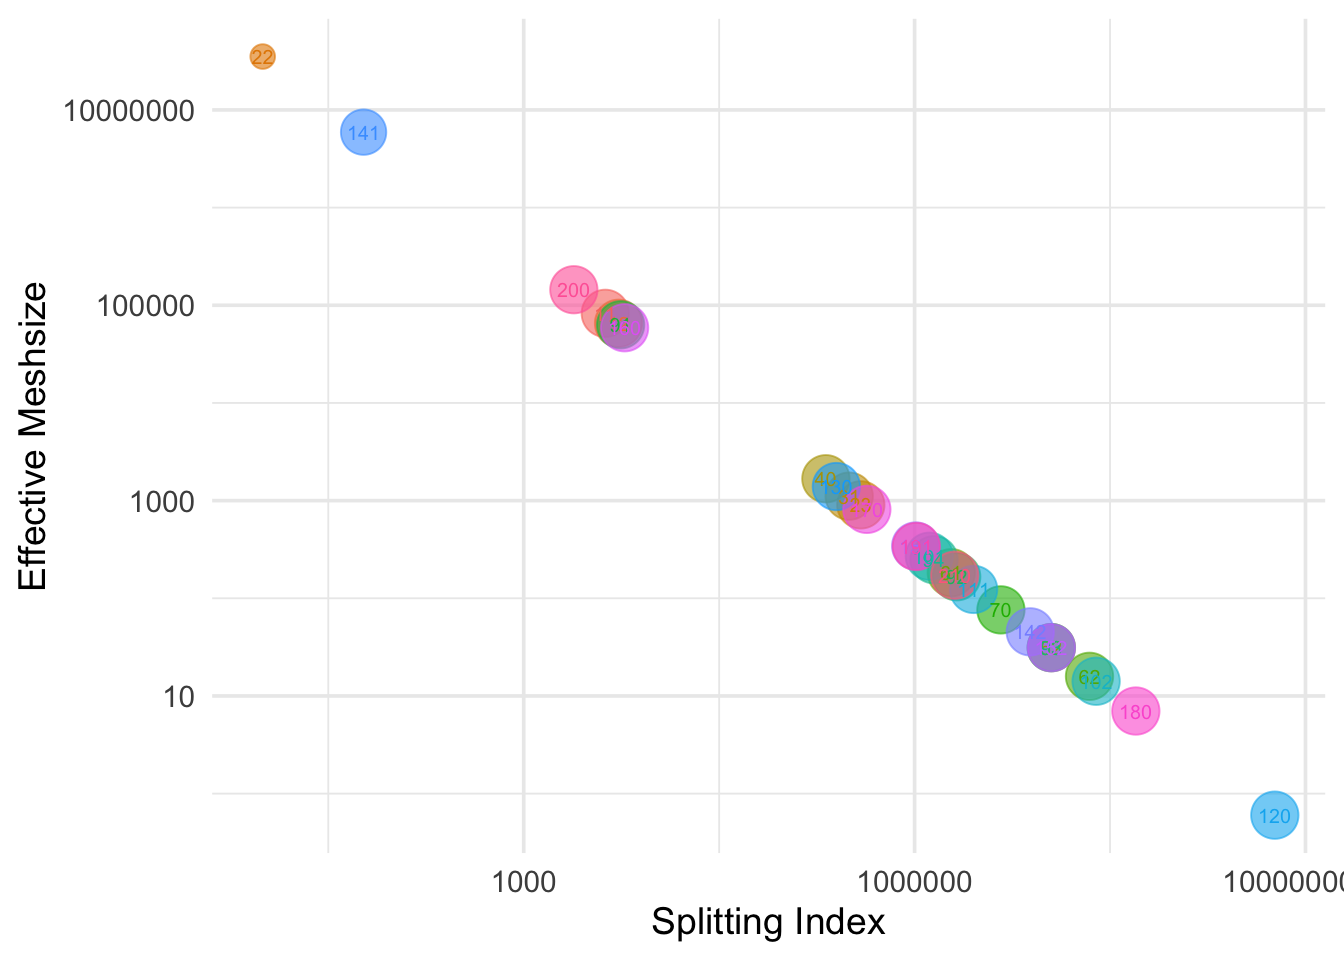
\includegraphics[keepaspectratio]{_main_files/figure-latex/plotSE-1.pdf}}
\caption{\label{fig:plotSE}Relazione tra Splitting index ed Effective Meshsize. Con i colori e le etichette di testo sono evidenziate le diverse classi geobotaniche.}
\end{figure}

\subsection{Morphological Spatial Pattern Analysis}\label{morphological-spatial-pattern-analysis-1}

La pianificazione territoriale nelle aree urbane richiede un approccio integrato che riconosca il ruolo cruciale della diversità ambientale nel sostenere la biodiversità locale.
Come evidenziato da Vilenica et al.~(2024), l'eterogeneità dell'habitat costituisce un fattore determinante per assicurare condizioni ecologiche ottimali alle specie autoctone e per preservare la continuità delle reti ecologiche territoriali.
L'applicazione della metodologia di Analisi dei Pattern Morfologici del Paesaggio (Morphological Spatial Pattern Analysis - MSPA) ha consentito la costruzione di un modello concettuale articolato su due componenti principali:

\begin{itemize}
\item
  Habitat: un sistema complesso derivante dall'integrazione di diverse categorie geobotaniche e tipologie di uso del suolo, che rappresenta l'insieme delle aree ad alta idoneità ecologica per le specie target.
\item
  Matrice di Background: le porzioni territoriali caratterizzate da condizioni ambientali generalmente subottimali, che fungono da spazio di transizione con limitata capacità di supporto per la fauna locale.
\end{itemize}

Questo approccio metodologico permette di identificare con precisione le aree prioritarie per la conservazione e di orientare le strategie di pianificazione verso la creazione di reti ecologiche funzionali ed efficaci.

Utilizzando come riferimento per l'identificazione della componente ``habitat'' la combinazione delle categorie geobotaniche delle formazioni boschive, delle aree a prateria, del sistema di siepi e filari arborei e dei corridoi fluviali e considerando come background tutte le altre è stata creata una carta a 8 livelli che esemplifica il risultato del modello MSPA (Fig. \ref{fig:mspaAll}).

\begin{figure}

{\centering 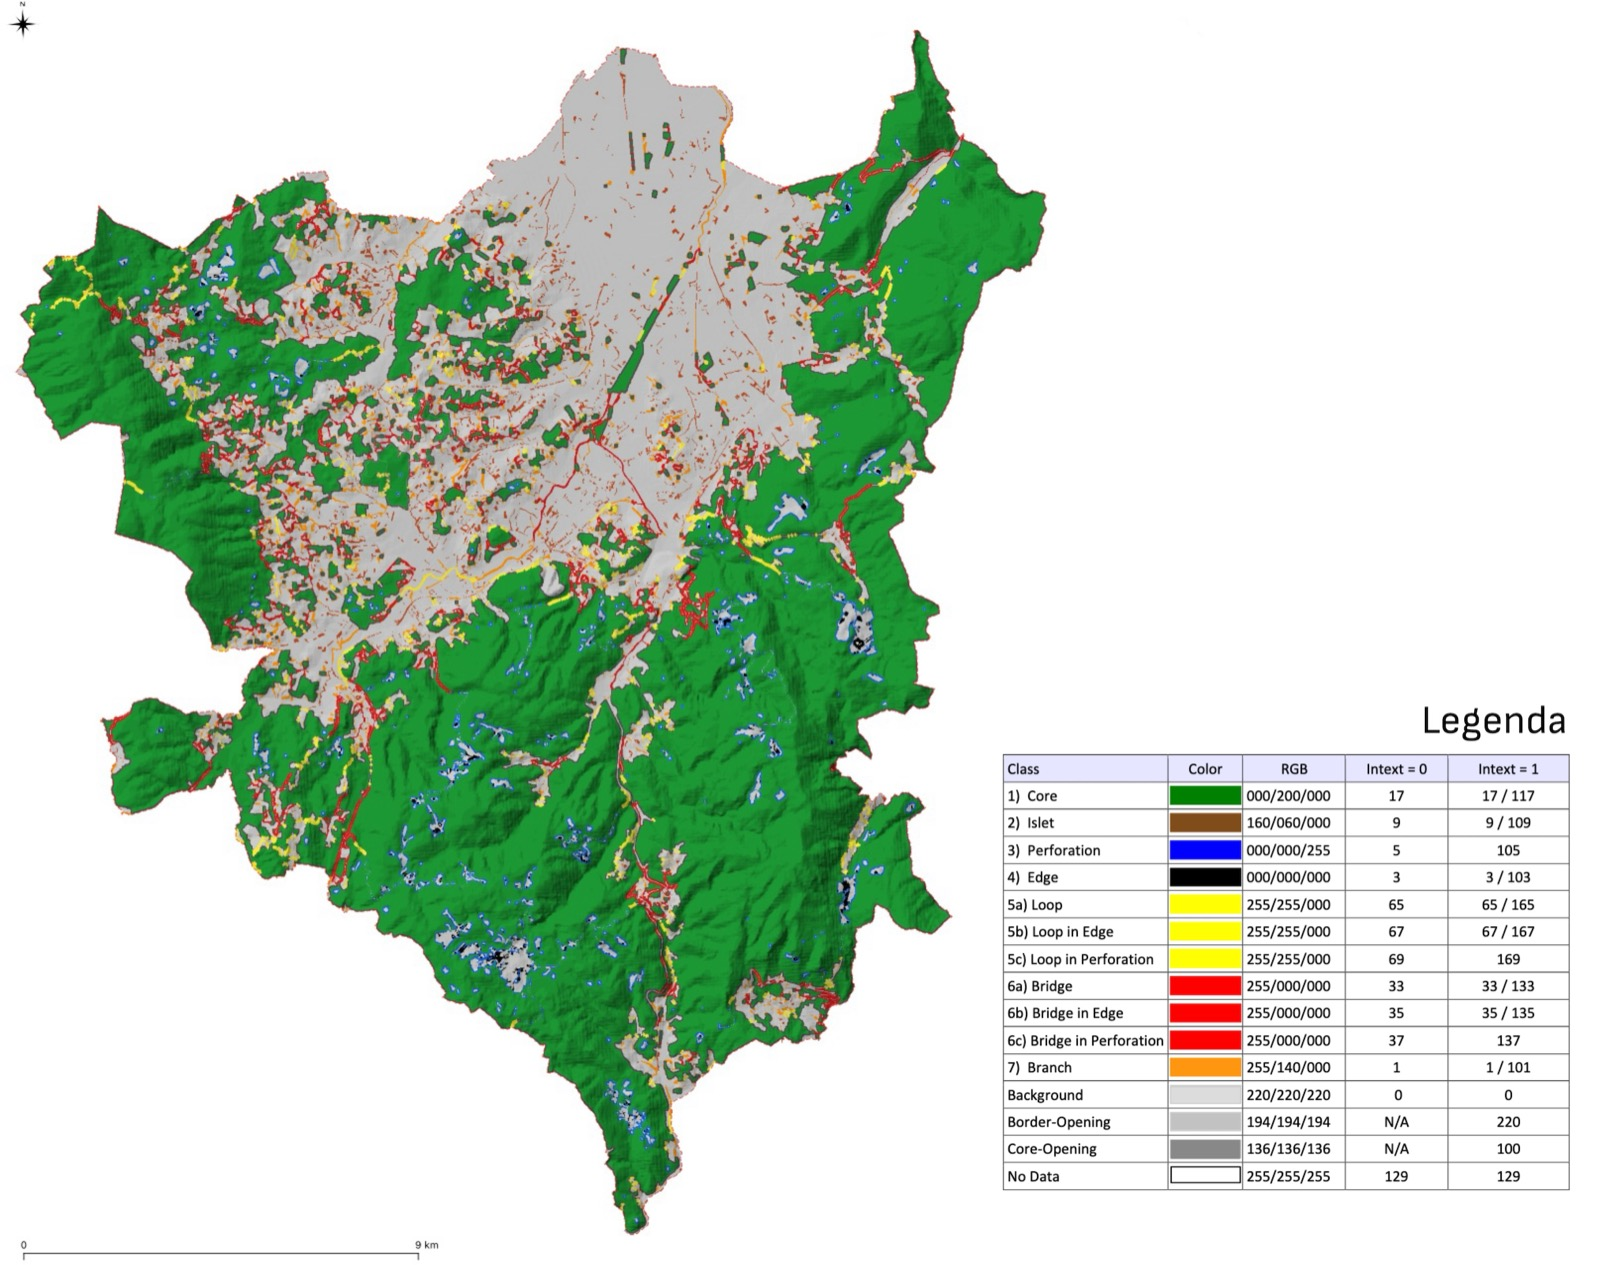
\includegraphics[width=\linewidth]{./figs/mspa8211_relazione} 

}

\caption{Mappa della distribuzione spaziale dei pattern morfologici identificati attraverso la riclassificazione delle categorie di uso del suolo. Nel modello presentato, la componente habitat è  costituita dall'aggregazione di quattro tipologie territoriali fondamentali: le formazioni boschive, le aree a prateria, il sistema delle siepi e dei filari arborei, e i corridoi fluviali con la relativa vegetazione ripariale.}\label{fig:mspaAll}
\end{figure}

Dall'analisi della carta emerge in modo chiaro che le aree Core (codice 17) rappresentano una porzione rilevante del territorio con circa il 70.8\% della superficie totale analizzata pur essendo distribuite in sole 555 patches.
Questo dato indica la presenza di ampie superfici di habitat continuo e di alta qualità ecologica, fondamentali per il mantenimento delle popolazioni faunistiche legate a questa particolare configurazione d'habitat.
L'elevato valore di Effective meshsize (33464983.54) e il basso Splitting index (6.88) confermano la buona connettività di queste aree.
Le aree Islet (isole di habitat), pur rappresentando solo l'1.4\% del territorio, sono suddivise in 2154 patches, indicando un'elevata dispersione di piccoli frammenti di habitat isolati.
Questo pattern suggerisce la necessità di intervenire con azioni mirati per migliorare la connettività ecologica e includere queste porzioni nel disegno di rete.
Contrariamente alle aree core, gli elementi di connettività rappresentati da Branch (rami), Bridge (ponti ecologici) e zone di Edge (margini) mostrano un più elevato grado di frammentazione: i rami sono distribuiti in 3.903 patches totali, ma occupano solo il 2.2\% del territorio, i ponti ecologici coprono appena il 3.8\% dell'area, mentre le zone di margine presentano 2749 patches per l'8\% della superficie totale (Tab. \ref{tab:mspaLecos}).

\begin{longtable}[]{@{}
  >{\raggedright\arraybackslash}p{(\linewidth - 14\tabcolsep) * \real{0.1250}}
  >{\raggedright\arraybackslash}p{(\linewidth - 14\tabcolsep) * \real{0.1250}}
  >{\raggedright\arraybackslash}p{(\linewidth - 14\tabcolsep) * \real{0.1250}}
  >{\raggedright\arraybackslash}p{(\linewidth - 14\tabcolsep) * \real{0.1250}}
  >{\raggedright\arraybackslash}p{(\linewidth - 14\tabcolsep) * \real{0.1250}}
  >{\raggedright\arraybackslash}p{(\linewidth - 14\tabcolsep) * \real{0.1250}}
  >{\raggedright\arraybackslash}p{(\linewidth - 14\tabcolsep) * \real{0.1250}}
  >{\raggedright\arraybackslash}p{(\linewidth - 14\tabcolsep) * \real{0.1250}}@{}}
\caption{\label{tab:mspaLecos} Risultati dell'analisi degli elementi strutturali basata sulle categorie di paesaggio ottenute dalla segmentazione con il metodo MSPA.}\tabularnewline
\toprule\noalign{}
\begin{minipage}[b]{\linewidth}\raggedright
\textbf{Code}
\end{minipage} & \begin{minipage}[b]{\linewidth}\raggedright
\textbf{Class}
\end{minipage} & \begin{minipage}[b]{\linewidth}\raggedright
\textbf{Number of Patches}
\end{minipage} & \begin{minipage}[b]{\linewidth}\raggedright
\textbf{Land cover}
\end{minipage} & \begin{minipage}[b]{\linewidth}\raggedright
\textbf{Landscape Proportion}
\end{minipage} & \begin{minipage}[b]{\linewidth}\raggedright
\textbf{Landscape division}
\end{minipage} & \begin{minipage}[b]{\linewidth}\raggedright
\textbf{Effective mesh size}
\end{minipage} & \begin{minipage}[b]{\linewidth}\raggedright
\textbf{Splitting index}
\end{minipage} \\
\midrule\noalign{}
\endfirsthead
\toprule\noalign{}
\begin{minipage}[b]{\linewidth}\raggedright
\textbf{Code}
\end{minipage} & \begin{minipage}[b]{\linewidth}\raggedright
\textbf{Class}
\end{minipage} & \begin{minipage}[b]{\linewidth}\raggedright
\textbf{Number of Patches}
\end{minipage} & \begin{minipage}[b]{\linewidth}\raggedright
\textbf{Land cover}
\end{minipage} & \begin{minipage}[b]{\linewidth}\raggedright
\textbf{Landscape Proportion}
\end{minipage} & \begin{minipage}[b]{\linewidth}\raggedright
\textbf{Landscape division}
\end{minipage} & \begin{minipage}[b]{\linewidth}\raggedright
\textbf{Effective mesh size}
\end{minipage} & \begin{minipage}[b]{\linewidth}\raggedright
\textbf{Splitting index}
\end{minipage} \\
\midrule\noalign{}
\endhead
\bottomrule\noalign{}
\endlastfoot
\textbf{100} & \textbf{Background} & 845 & 4773580 & 0.021 & 0.99999 & 1847.47 & 124628.96 \\
\textbf{220} & \textbf{Background} & 1902 & 15054956 & 0.065 & 0.99994 & 14621.21 & 15747.51 \\
\textbf{1} & \textbf{Branch} & 3447 & 4772208 & 0.021 & 1.00000 & 146.36 & 1573199.05 \\
\textbf{101} & \textbf{Branch} & 456 & 336728 & 0.001 & 1.00000 & 2.55 & 90337629.04 \\
\textbf{33} & \textbf{Bridge} & 743 & 3603264 & 0.016 & 1.00000 & 268.86 & 856372.24 \\
\textbf{35} & \textbf{Bridge} & 1098 & 4699884 & 0.020 & 1.00000 & 346.43 & 664638.53 \\
\textbf{133} & \textbf{Bridge} & 54 & 177772 & 0.001 & 1.00000 & 7.52 & 30610155.08 \\
\textbf{135} & \textbf{Bridge} & 33 & 125048 & 0.001 & 1.00000 & 2.73 & 84403524.24 \\
\textbf{137} & \textbf{Bridge} & 72 & 167972 & 0.001 & 1.00000 & 2.49 & 92301359.19 \\
\textbf{17} & \textbf{Core} & 555 & 162900696 & 0.708 & 0.85466 & 33464983.54 & 6.88 \\
\textbf{117} & \textbf{Core} & 41 & 51352 & 0.000 & 1.00000 & 1.64 & 140300693.50 \\
\textbf{3} & \textbf{Edge} & 2701 & 18394992 & 0.080 & 0.99998 & 4193.94 & 54900.14 \\
\textbf{103} & \textbf{Edge} & 48 & 93884 & 0.000 & 1.00000 & 2.17 & 106259923.10 \\
\textbf{9} & \textbf{Islet} & 2068 & 3169908 & 0.014 & 1.00000 & 87.59 & 2628732.13 \\
\textbf{109} & \textbf{Islet} & 86 & 67816 & 0.000 & 1.00000 & 0.85 & 271760067.21 \\
\textbf{65} & \textbf{Loop} & 400 & 1651692 & 0.007 & 1.00000 & 106.83 & 2155286.51 \\
\textbf{67} & \textbf{Loop} & 662 & 2453920 & 0.011 & 1.00000 & 95.10 & 2421150.40 \\
\textbf{165} & \textbf{Loop} & 243 & 504308 & 0.002 & 1.00000 & 16.06 & 14332723.55 \\
\textbf{169} & \textbf{Loop} & 393 & 1897672 & 0.008 & 1.00000 & 123.74 & 1860682.66 \\
\textbf{105} & \textbf{Perforation} & 942 & 5350016 & 0.023 & 1.00000 & 405.21 & 568221.55 \\
\end{longtable}

Riproponendo questa stessa analisi nel contesto territoriale della fascia del piano collinare che si estende per circa 128 \(km^2\) i risultati hanno fornito un quadro con alcuni rilevanti differenze rispetto alla situazione precedente (Fig. \ref{fig:mspaCollina}).

\begin{figure}

{\centering 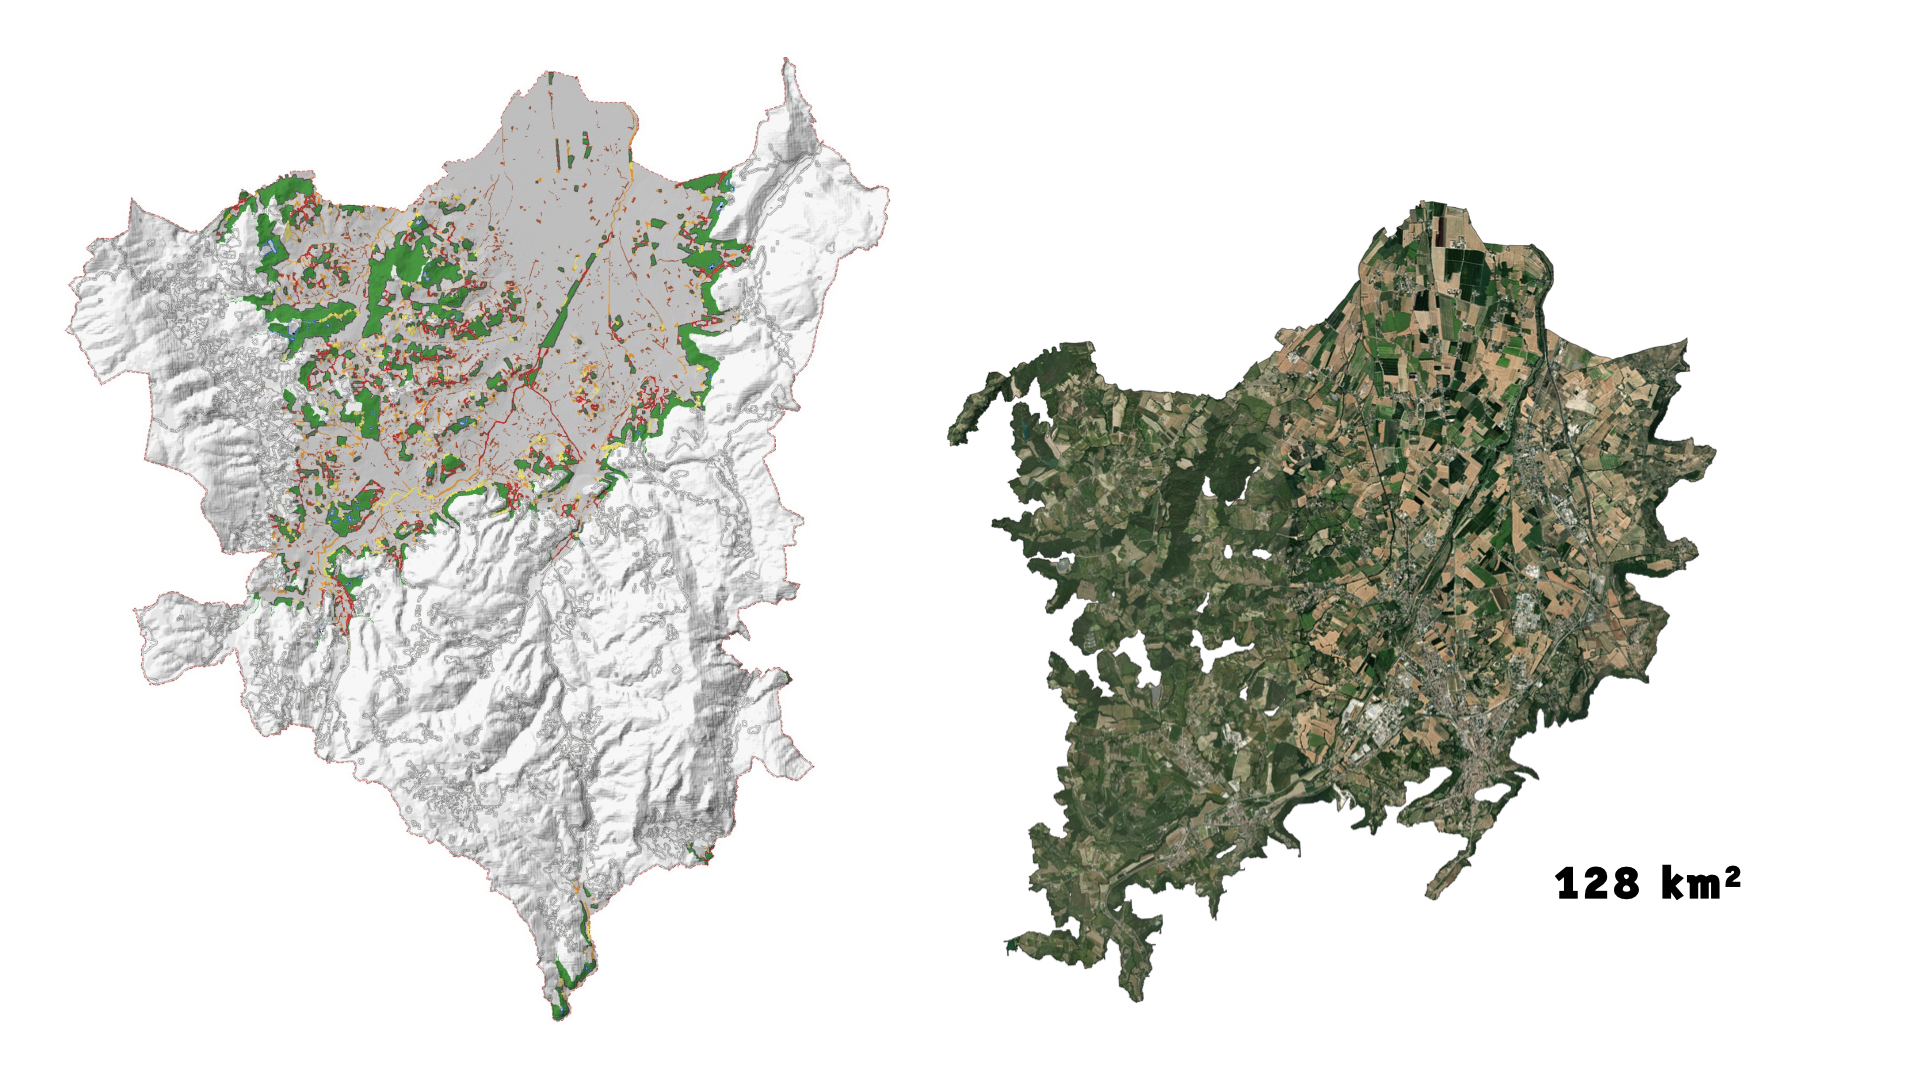
\includegraphics[width=\linewidth]{./figs/mspa8211_collina} 

}

\caption{Mappa della distribuzione spaziale dei pattern morfologici nel piano collinare (per l'interpretazione dei colori vedi legenda figura sopra). A destra l'immagine satellitare dell'area.}\label{fig:mspaCollina}
\end{figure}

Il pattern 17 (Core) mantiene la sua importanza strutturale, rappresentando ancora il 38.8\% del territorio ed essendo distribuito in 480 patches.
Rispetto all'analisi del contesto comunale complessivo, si nota una significativa riduzione della proporzione territoriale di questa classe (dal 70.8\% al 38.8\%) e un aumento della frammentazione, con conseguente diminuzione dell'Effective mesh size (290878.52) e aumento dello Splitting index (157.79).
Nonostante ciò, le aree Core mantengono un grado connettività interna che necessita di essere rafforzato attraverso il potenzialmento delle connessioni.
Gli elementi di connessione lineare interrotti (Pattern 1/101) e che al momento non connettono porzioni di habitat sono presenti in un numero di patches superiore a 2000, con un'occupazione percentuale dell'8.1.
Le aree Edge (Pattern 3) raggiungono il 19.5\% del territorio in 1208 patches, rappresentando un sostanziale incremento rispetto all'analisi generale e mettendo in luce una maggiore esposizione delle aree di habitat alle pressioni esterne.
Interessante e promettente il fatto che le Islet (Pattern 9) costituiscano il 7.3\% dell'area e che siano ripartite in 1836 patches, con un Splitting index (88213.18) che, pur rimanendo elevato, indica una minor dispersione rispetto all'analisi generale.
Questo suggerisce la presenza di clusters di piccoli habitat isolati piuttosto che veri e propri frammenti completamente dispersi (Tab. \ref{tab:mspaCollina}).

\begin{longtable}[]{@{}
  >{\raggedright\arraybackslash}p{(\linewidth - 12\tabcolsep) * \real{0.1429}}
  >{\raggedright\arraybackslash}p{(\linewidth - 12\tabcolsep) * \real{0.1429}}
  >{\raggedright\arraybackslash}p{(\linewidth - 12\tabcolsep) * \real{0.1429}}
  >{\raggedright\arraybackslash}p{(\linewidth - 12\tabcolsep) * \real{0.1429}}
  >{\raggedright\arraybackslash}p{(\linewidth - 12\tabcolsep) * \real{0.1429}}
  >{\raggedright\arraybackslash}p{(\linewidth - 12\tabcolsep) * \real{0.1429}}
  >{\raggedright\arraybackslash}p{(\linewidth - 12\tabcolsep) * \real{0.1429}}@{}}
\caption{\label{tab:mspaCollina} Risultati dell'analisi degli elementi strutturali basata sulle categorie di paesaggio ottenute dalla segmentazione con il metodo MSPA applicate alla fascia collinare.}\tabularnewline
\toprule\noalign{}
\begin{minipage}[b]{\linewidth}\raggedright
\textbf{Code}
\end{minipage} & \begin{minipage}[b]{\linewidth}\raggedright
\textbf{Number of Patches}
\end{minipage} & \begin{minipage}[b]{\linewidth}\raggedright
\textbf{Land cover}
\end{minipage} & \begin{minipage}[b]{\linewidth}\raggedright
\textbf{Landscape Proportion}
\end{minipage} & \begin{minipage}[b]{\linewidth}\raggedright
\textbf{Landscape division}
\end{minipage} & \begin{minipage}[b]{\linewidth}\raggedright
\textbf{Splitting index}
\end{minipage} & \begin{minipage}[b]{\linewidth}\raggedright
\textbf{Effective mesh size}
\end{minipage} \\
\midrule\noalign{}
\endfirsthead
\toprule\noalign{}
\begin{minipage}[b]{\linewidth}\raggedright
\textbf{Code}
\end{minipage} & \begin{minipage}[b]{\linewidth}\raggedright
\textbf{Number of Patches}
\end{minipage} & \begin{minipage}[b]{\linewidth}\raggedright
\textbf{Land cover}
\end{minipage} & \begin{minipage}[b]{\linewidth}\raggedright
\textbf{Landscape Proportion}
\end{minipage} & \begin{minipage}[b]{\linewidth}\raggedright
\textbf{Landscape division}
\end{minipage} & \begin{minipage}[b]{\linewidth}\raggedright
\textbf{Splitting index}
\end{minipage} & \begin{minipage}[b]{\linewidth}\raggedright
\textbf{Effective mesh size}
\end{minipage} \\
\midrule\noalign{}
\endhead
\bottomrule\noalign{}
\endlastfoot
\textbf{1} & 2003 & 3699675.0 & 0.081 & 0.99998 & 61253.00 & 749.31 \\
\textbf{3} & 1208 & 8962200.0 & 0.195 & 0.99989 & 9164.26 & 5008.34 \\
\textbf{9} & 1836 & 3332700.0 & 0.073 & 0.99999 & 88213.18 & 520.30 \\
\textbf{17} & 480 & 17809650.0 & 0.388 & 0.99366 & 157.79 & 290878.52 \\
\textbf{33} & 425 & 2309400.0 & 0.050 & 0.99998 & 42137.97 & 1089.23 \\
\textbf{35} & 613 & 2222550.0 & 0.048 & 0.99999 & 117313.83 & 391.24 \\
\textbf{65} & 162 & 881775.0 & 0.019 & 0.99999 & 105352.23 & 435.66 \\
\textbf{67} & 238 & 805725.0 & 0.018 & 1.00000 & 437334.29 & 104.95 \\
\textbf{100} & 50 & 274950.0 & 0.006 & 1.00000 & 236835.06 & 193.80 \\
\textbf{101} & 8 & 6525.0 & 0.000 & 1.00000 & 303736643.07 & 0.15 \\
\textbf{105} & 72 & 424575.0 & 0.009 & 1.00000 & 434548.40 & 105.62 \\
\textbf{165} & 16 & 26550.0 & 0.001 & 1.00000 & 19834089.66 & 2.31 \\
\textbf{169} & 36 & 79650.0 & 0.002 & 1.00000 & 8332382.88 & 5.51 \\
\textbf{220} & 730 & 5061825.0 & 0.110 & 0.99979 & 4837.00 & 9488.89 \\
\end{longtable}

\subsection{Contributo allo sviluppo delle schede di Agenda Urbana}\label{contributo-allo-sviluppo-delle-schede-di-agenda-urbana}

Alcuni dei prodotti cartografici elaborati nel corso del presente studio hanno già trovato applicazione in specifiche valutazioni e analisi condotte nell'ambito della progettazione degli interventi previsti per Agenda Urbana.
In particolare, durante le fasi preliminari per l'individuazione delle aree da coinvolgere e della prioritizzazione degli interventi alcune cartografie sono state discusse e sottoposte a valutazione sui tavoli tecnici istituzionali per la definizione della strategia di intervento territoriale e per le azioni di riconnessione e ricucitura del sistema di mobilità dolce.

In particolare, le tavole consegnate hanno riguardato il livello di frammentazione del territorio, la vocazionalità generale e la relativa biopermeabilità, le aree verdi e quelle di possibile pianificazione e progettazione degli interventi, anche in sinergia con il progetto lifeIMAGINE (LIFE19 IPE/IT/000015).

A seguire vengono proposte alcune delle tavole più significative.

\begin{figure}

{\centering 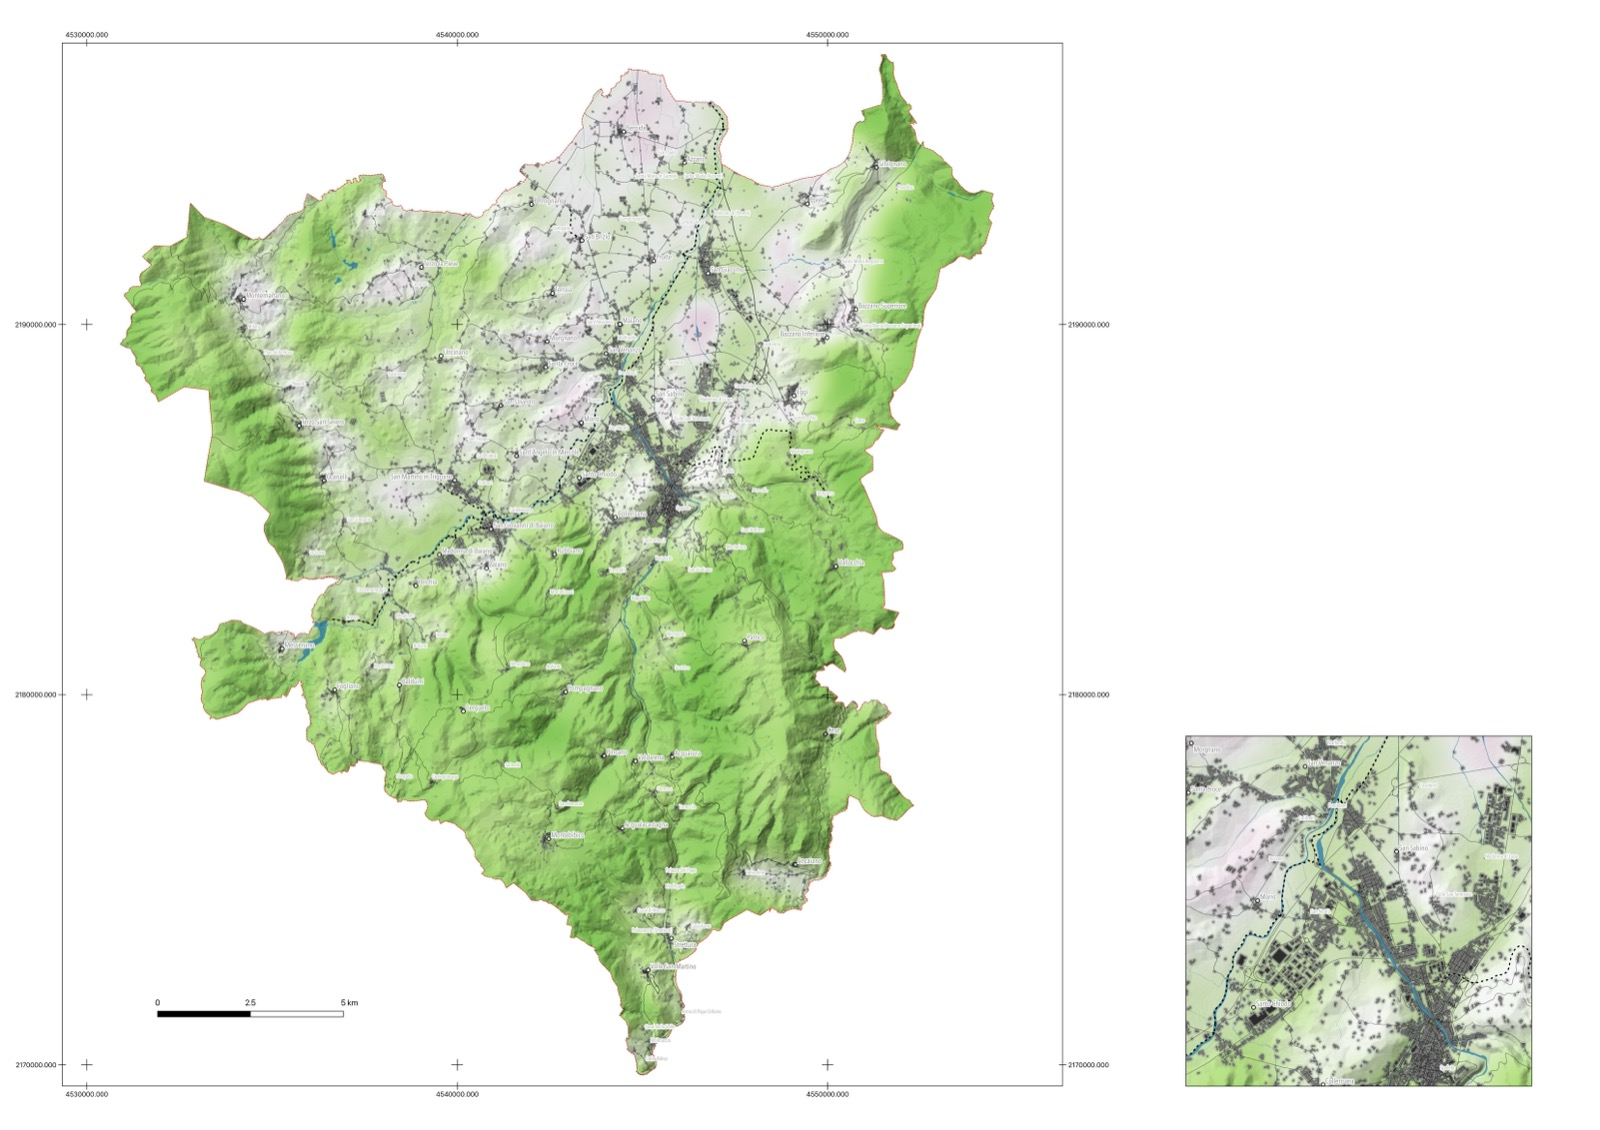
\includegraphics[width=\linewidth]{./figs/agendaUrbana/mappaSuitability20240619} 

}

\caption{Mappa della vocazionalità}\label{fig:agUsuit}
\end{figure}

\begin{figure}

{\centering 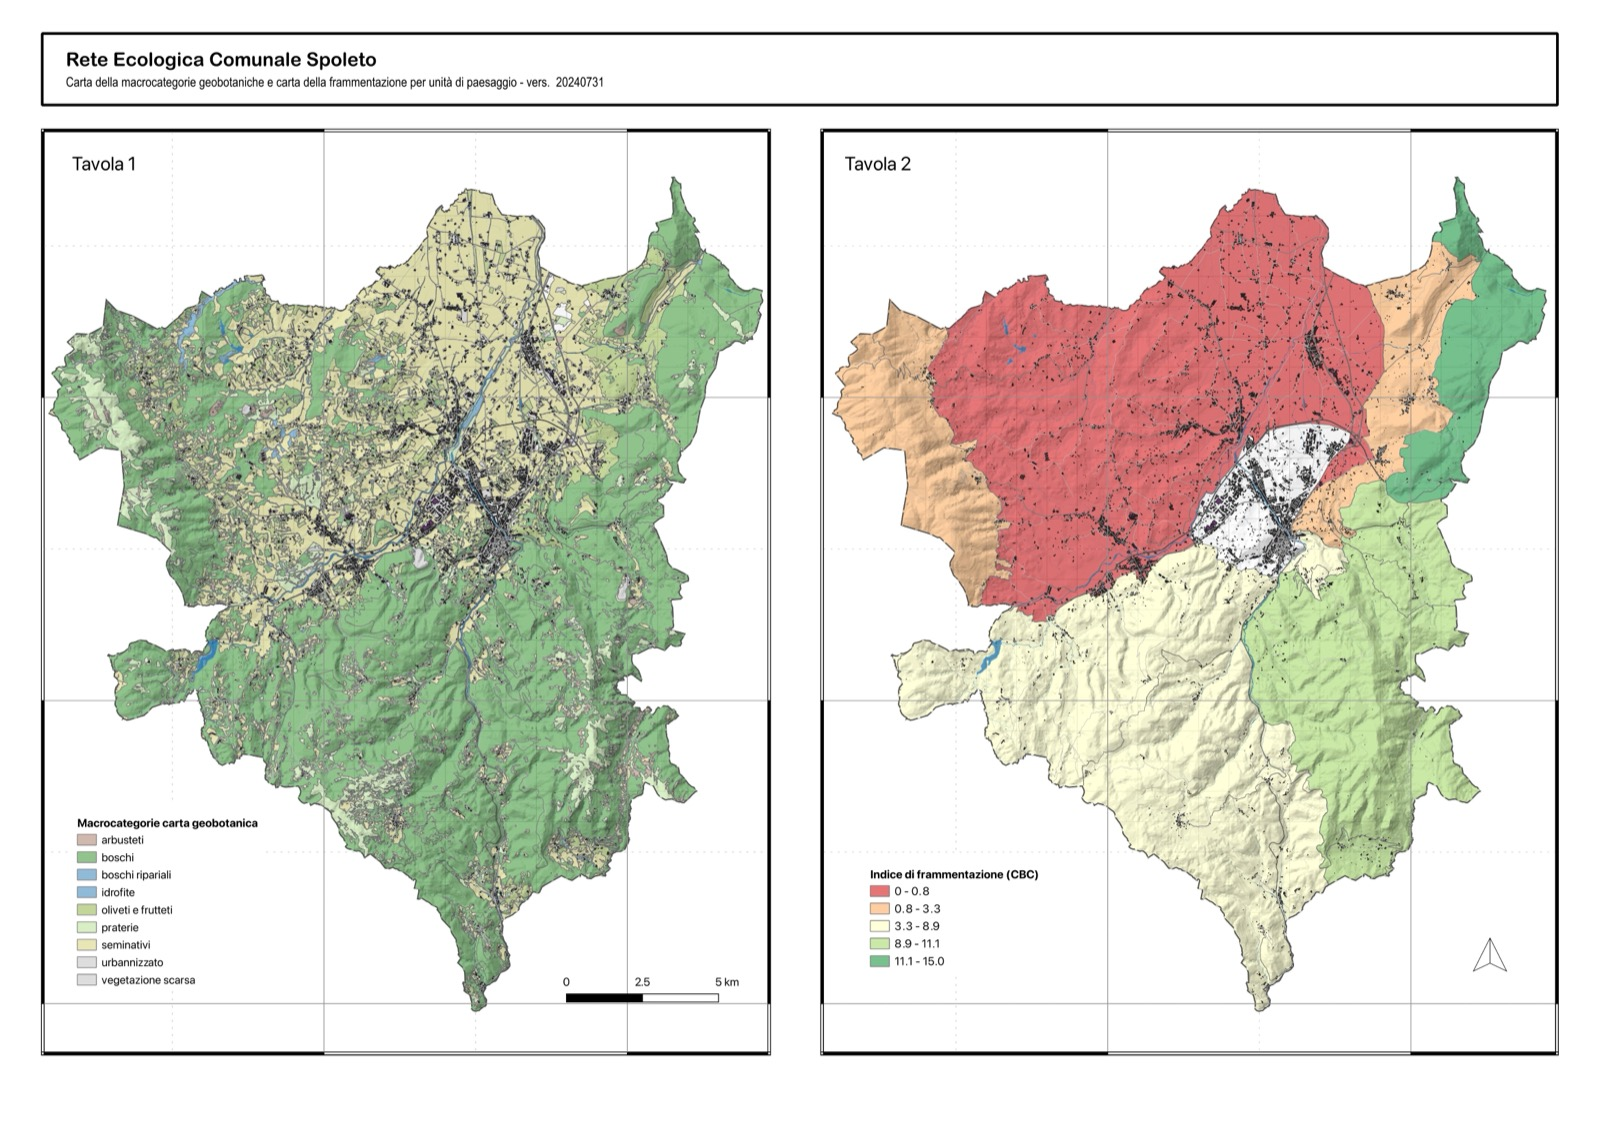
\includegraphics[width=\linewidth]{./figs/agendaUrbana/cartaFrammentazione} 

}

\caption{Mappa della frammentazione}\label{fig:agUframm}
\end{figure}

\begin{figure}

{\centering 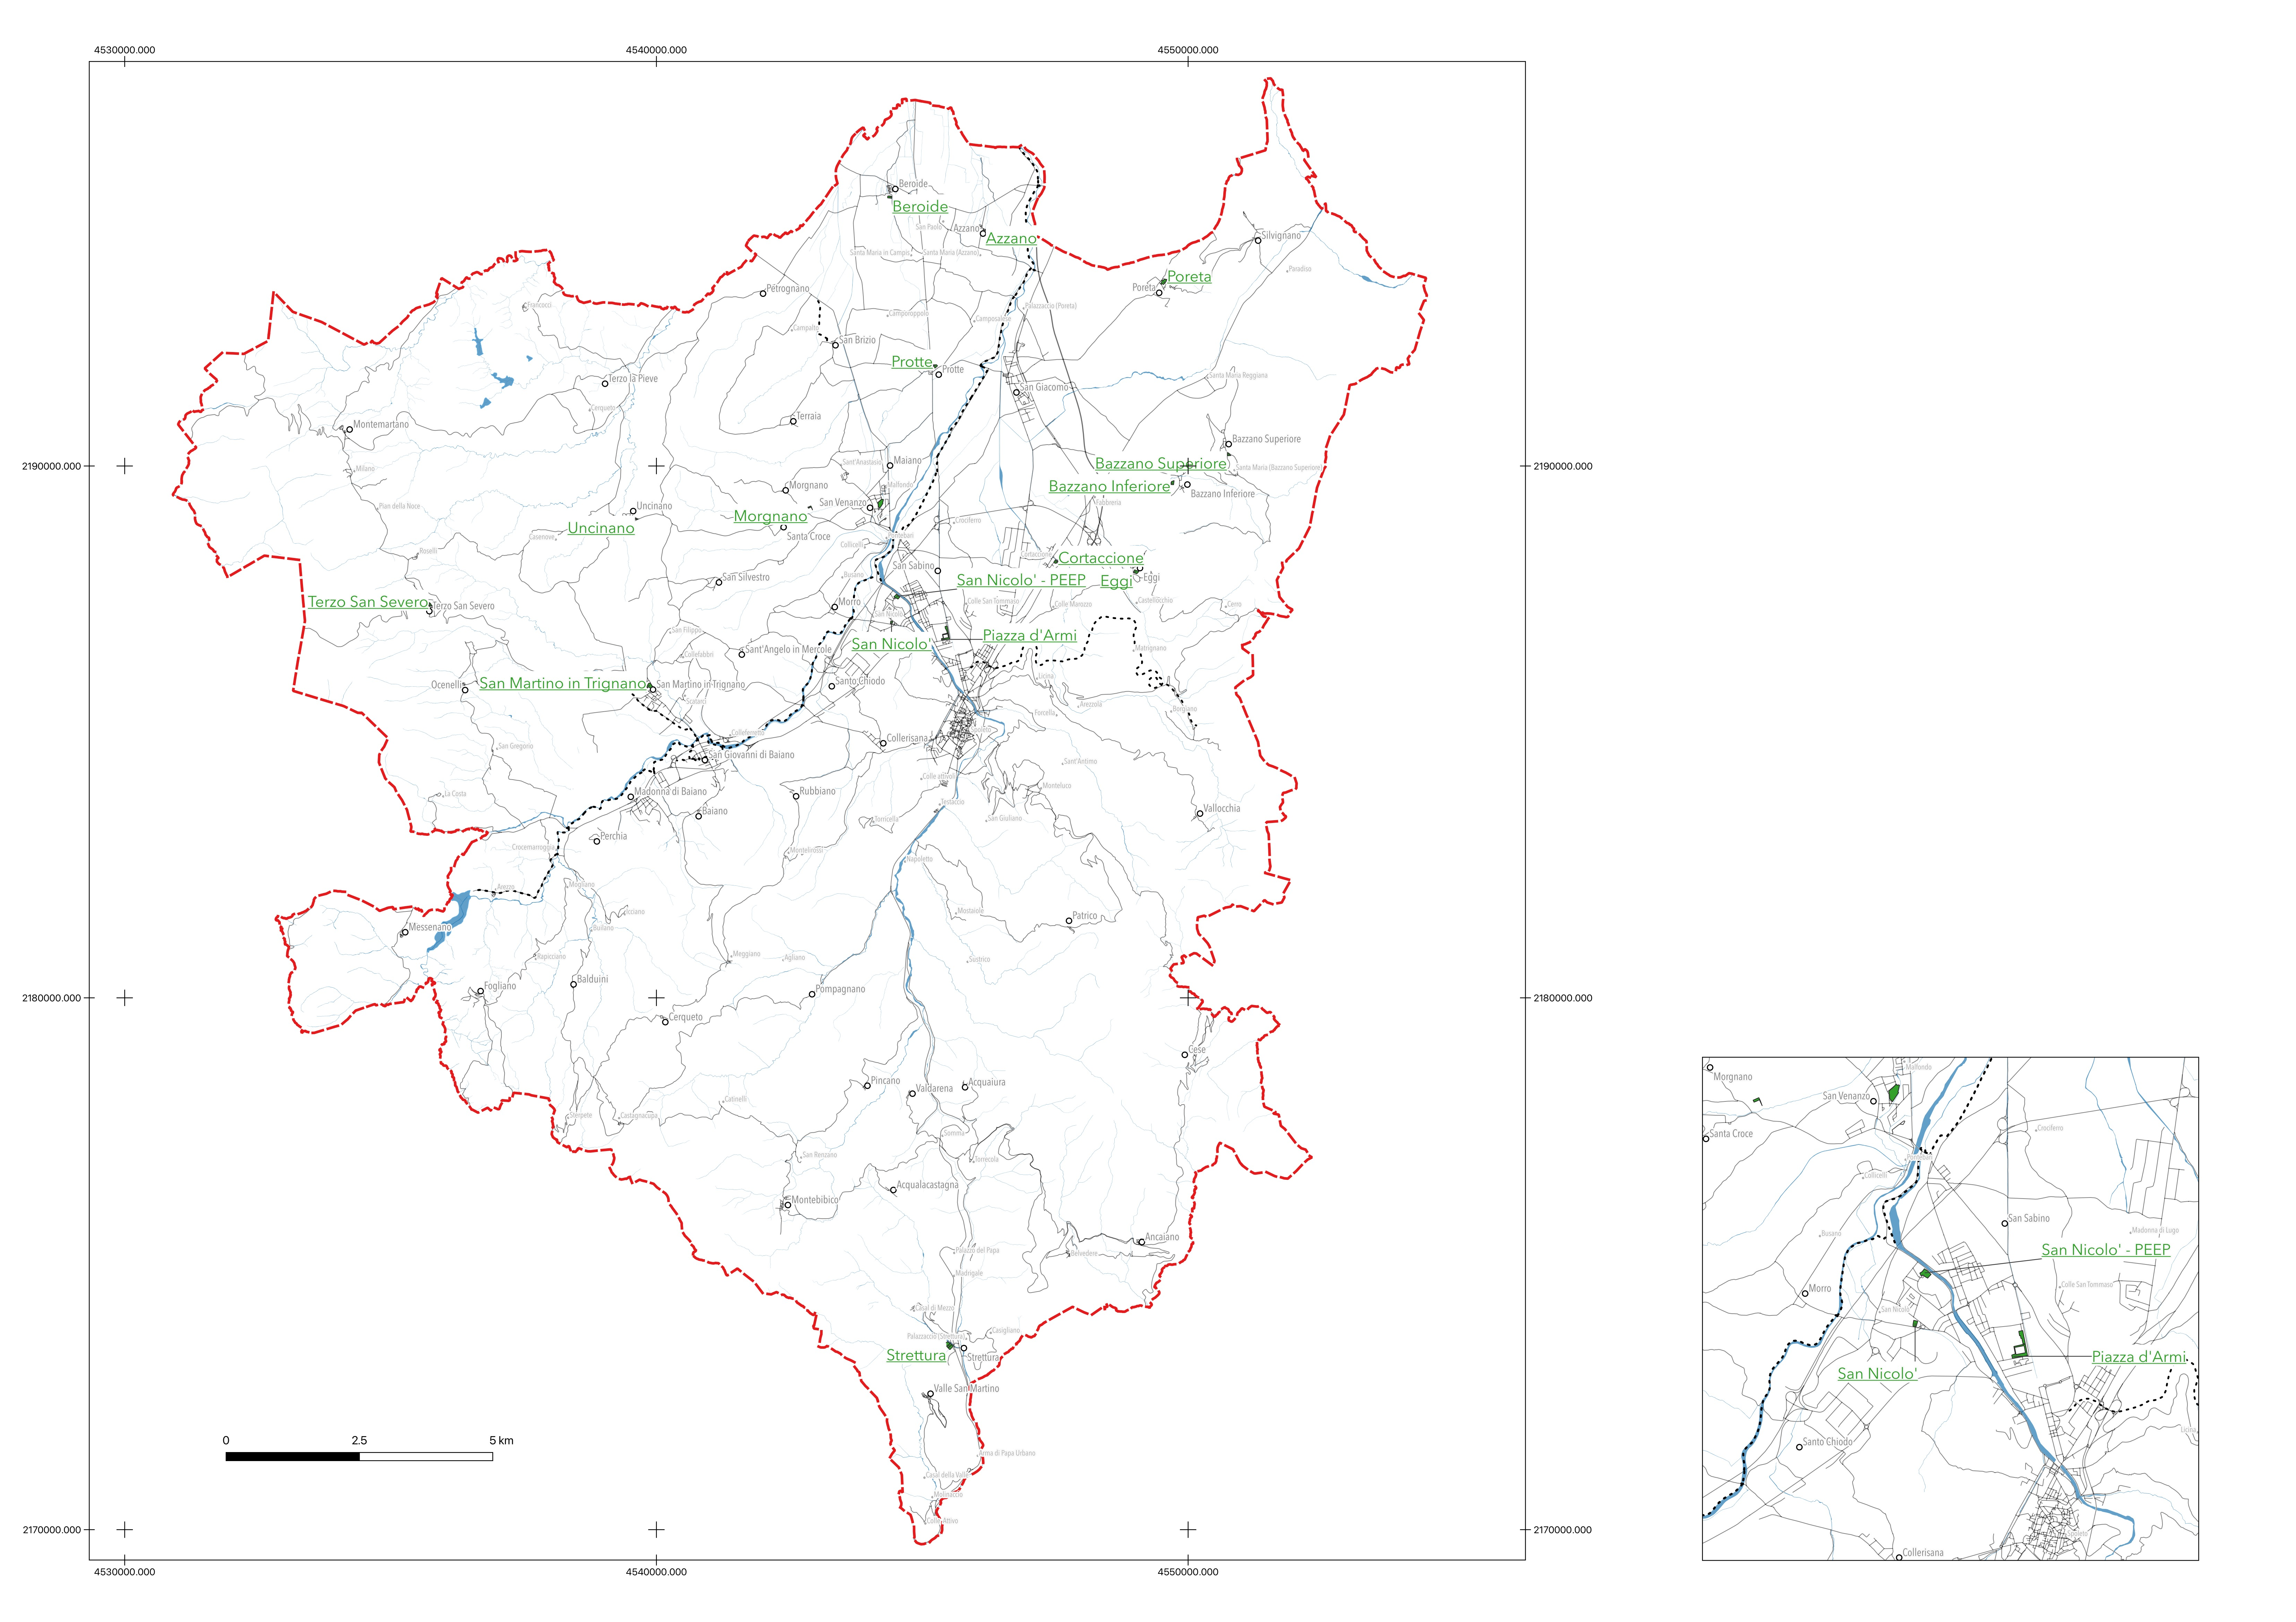
\includegraphics[width=\linewidth]{./figs/agendaUrbana/mappaVerdiAttrezzati20240619} 

}

\caption{Mappa del verde attrezzato}\label{fig:agUverdi}
\end{figure}

\begin{figure}

{\centering 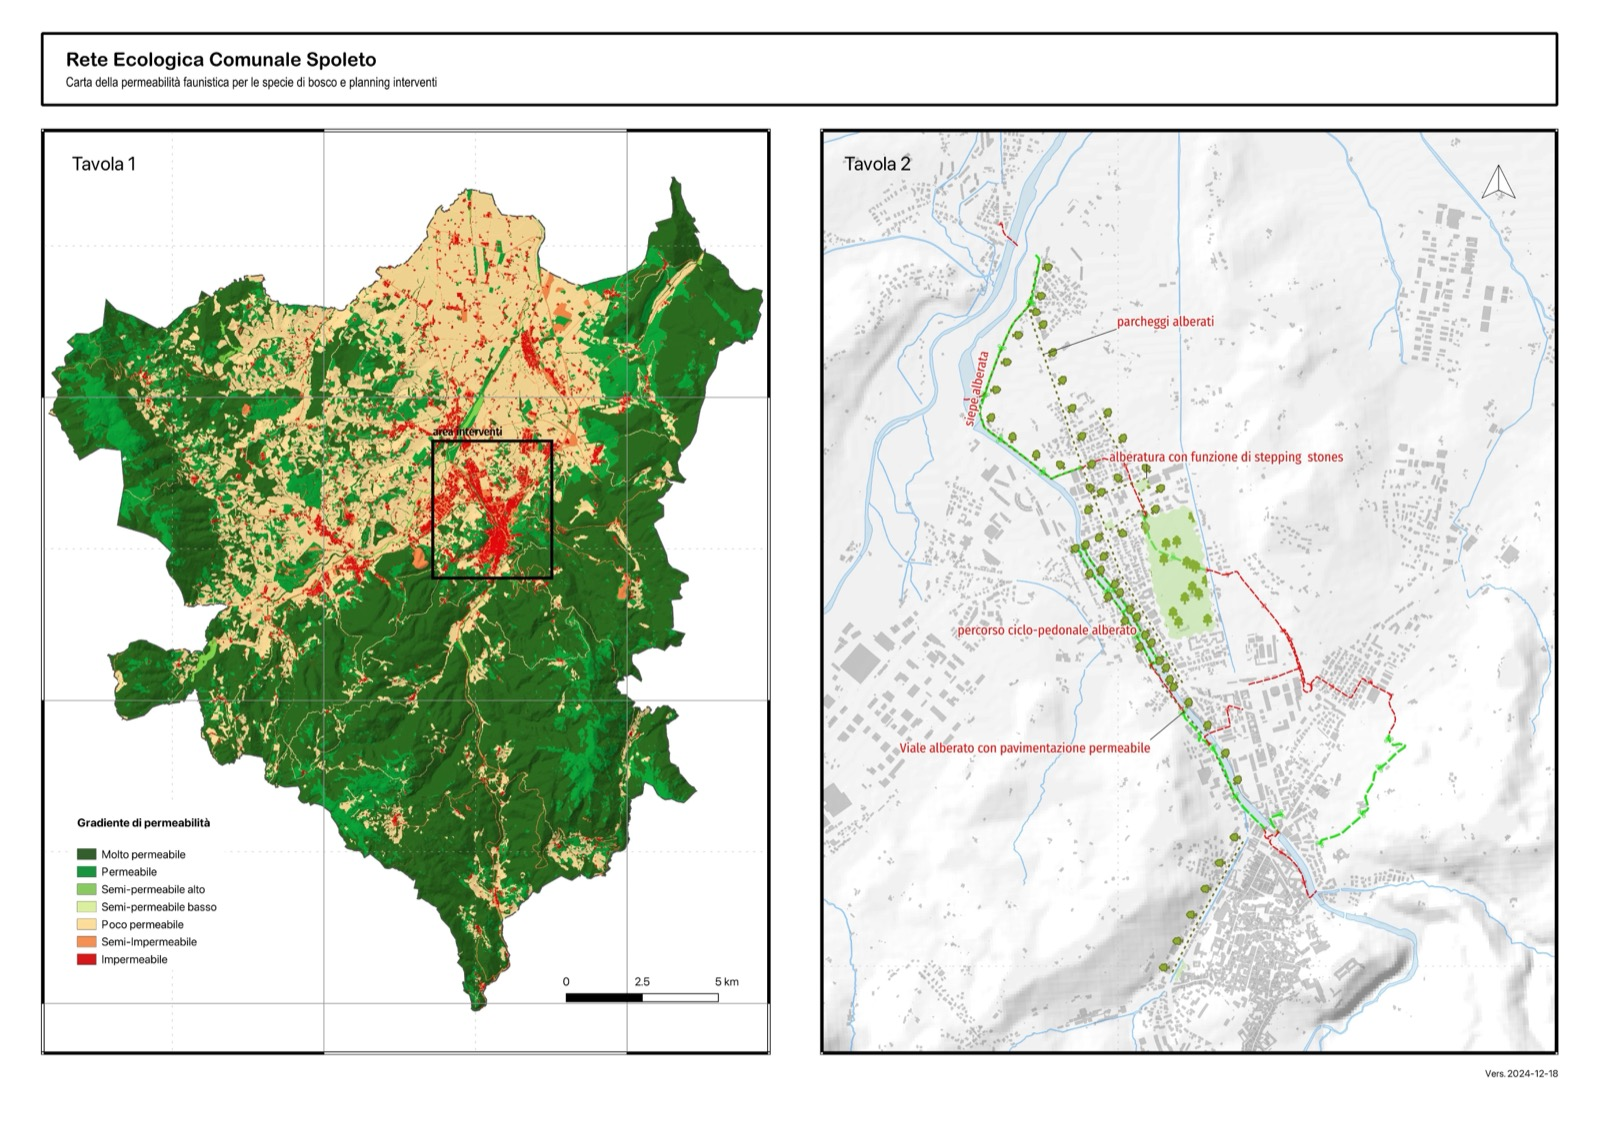
\includegraphics[width=\linewidth]{./figs/agendaUrbana/tavolaAgendaUrbana_BiopermInterventi20241218} 

}

\caption{Mappa con focus sull'area di possibile intervento}\label{fig:agUbioperm}
\end{figure}

\begin{figure}

{\centering 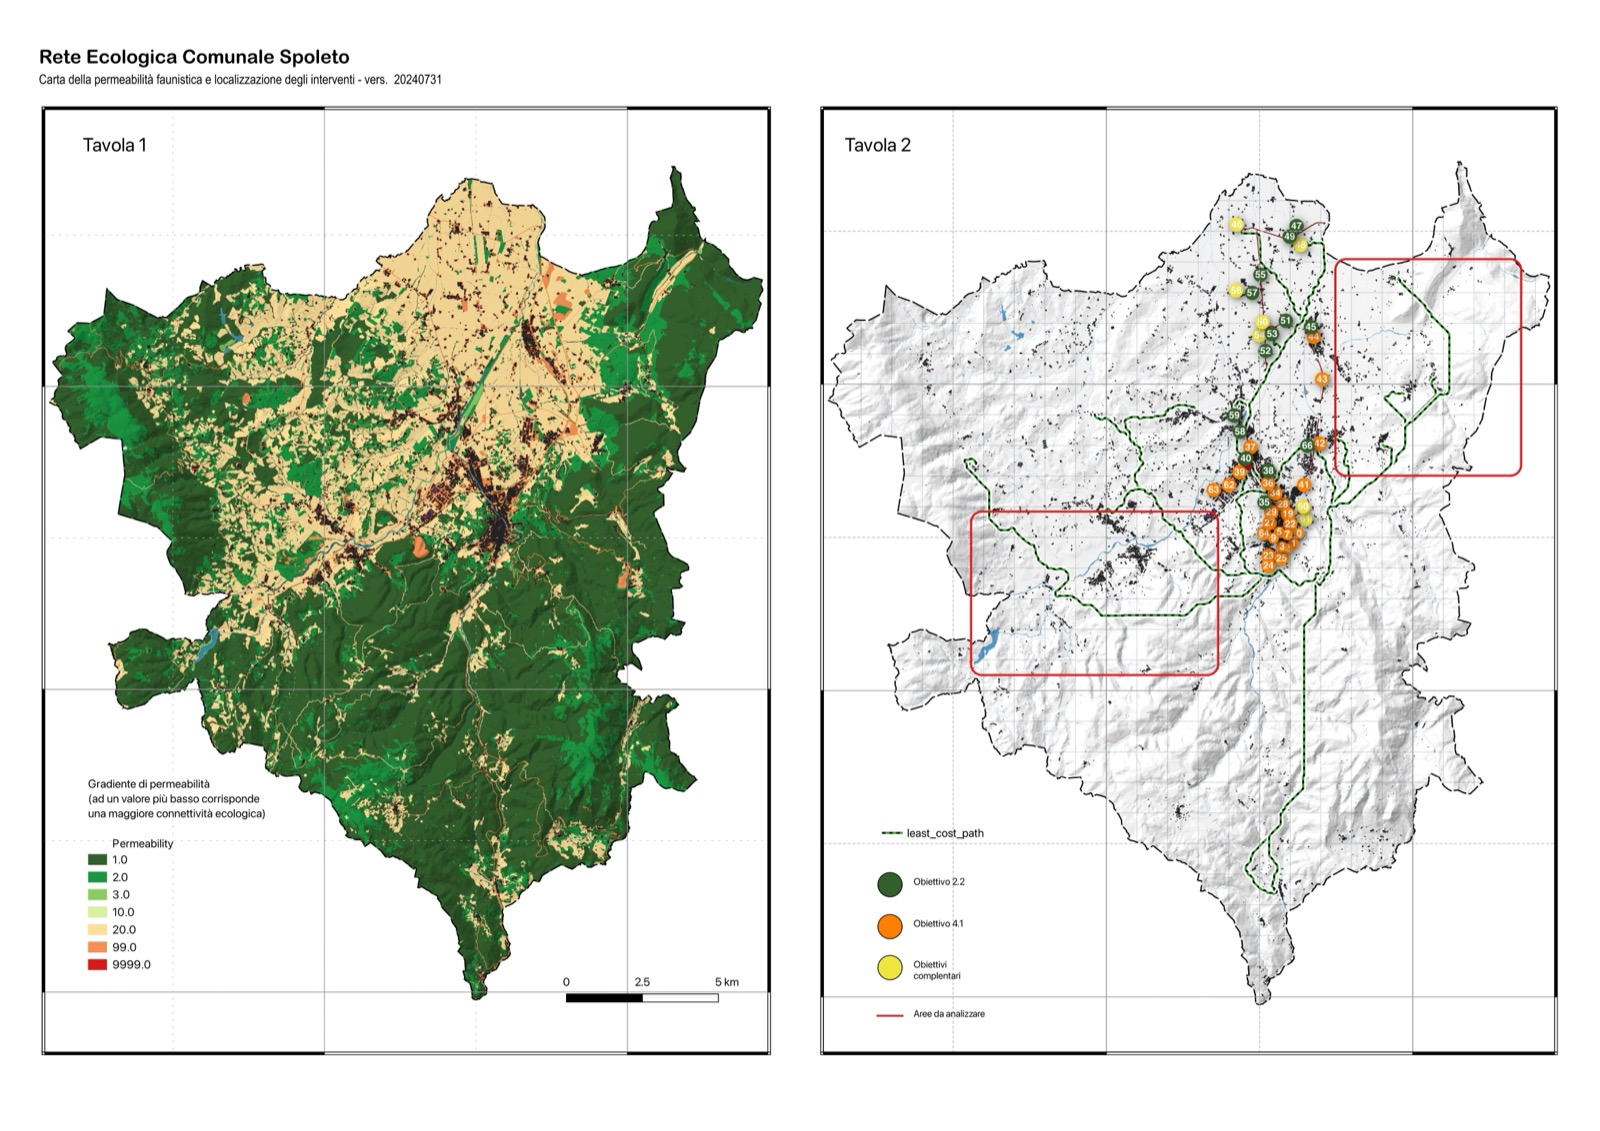
\includegraphics[width=\linewidth]{./figs/agendaUrbana/tavolaAgendaUrbana20240731} 

}

\caption{Mappa con interventi potenziali e linee di connessione faunistica potenziale}\label{fig:agUintev}
\end{figure}

\begin{figure}

{\centering 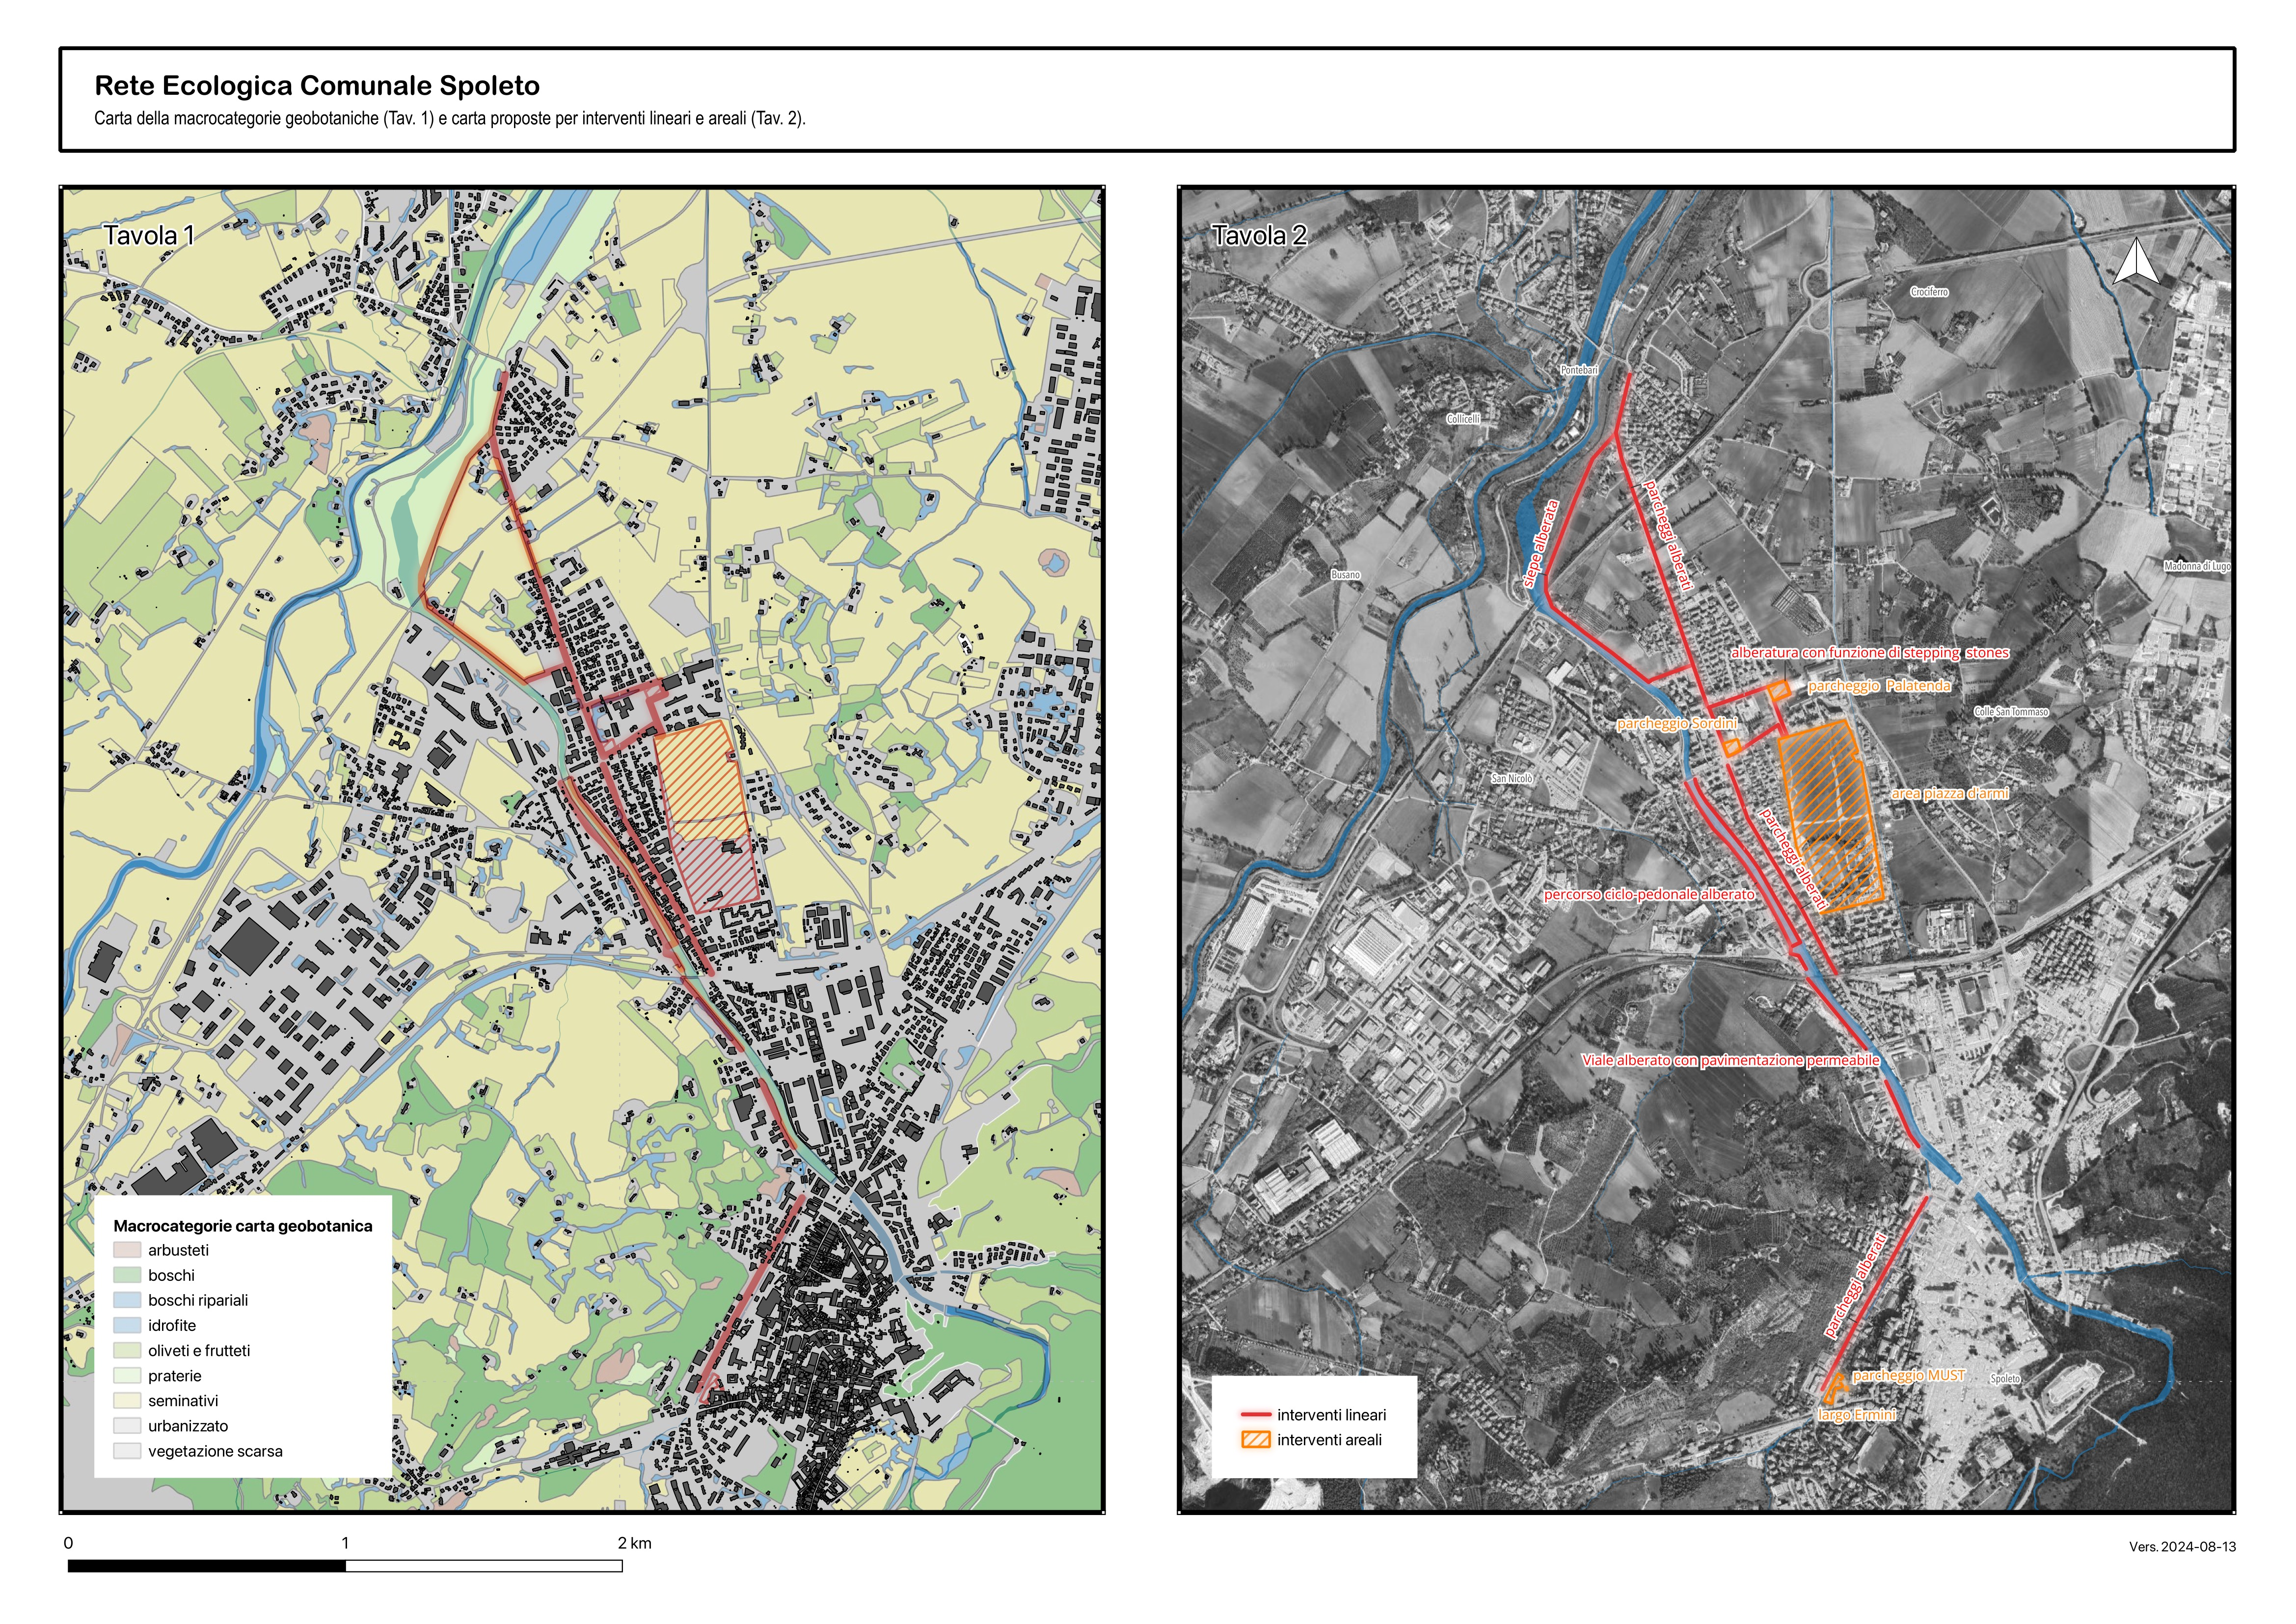
\includegraphics[width=\linewidth]{./figs/agendaUrbana/tavolaAgendaUrbana20240813} 

}

\caption{Mappa interventi lineari e areali potenziali}\label{fig:agUintevFocus}
\end{figure}

\begin{figure}

{\centering 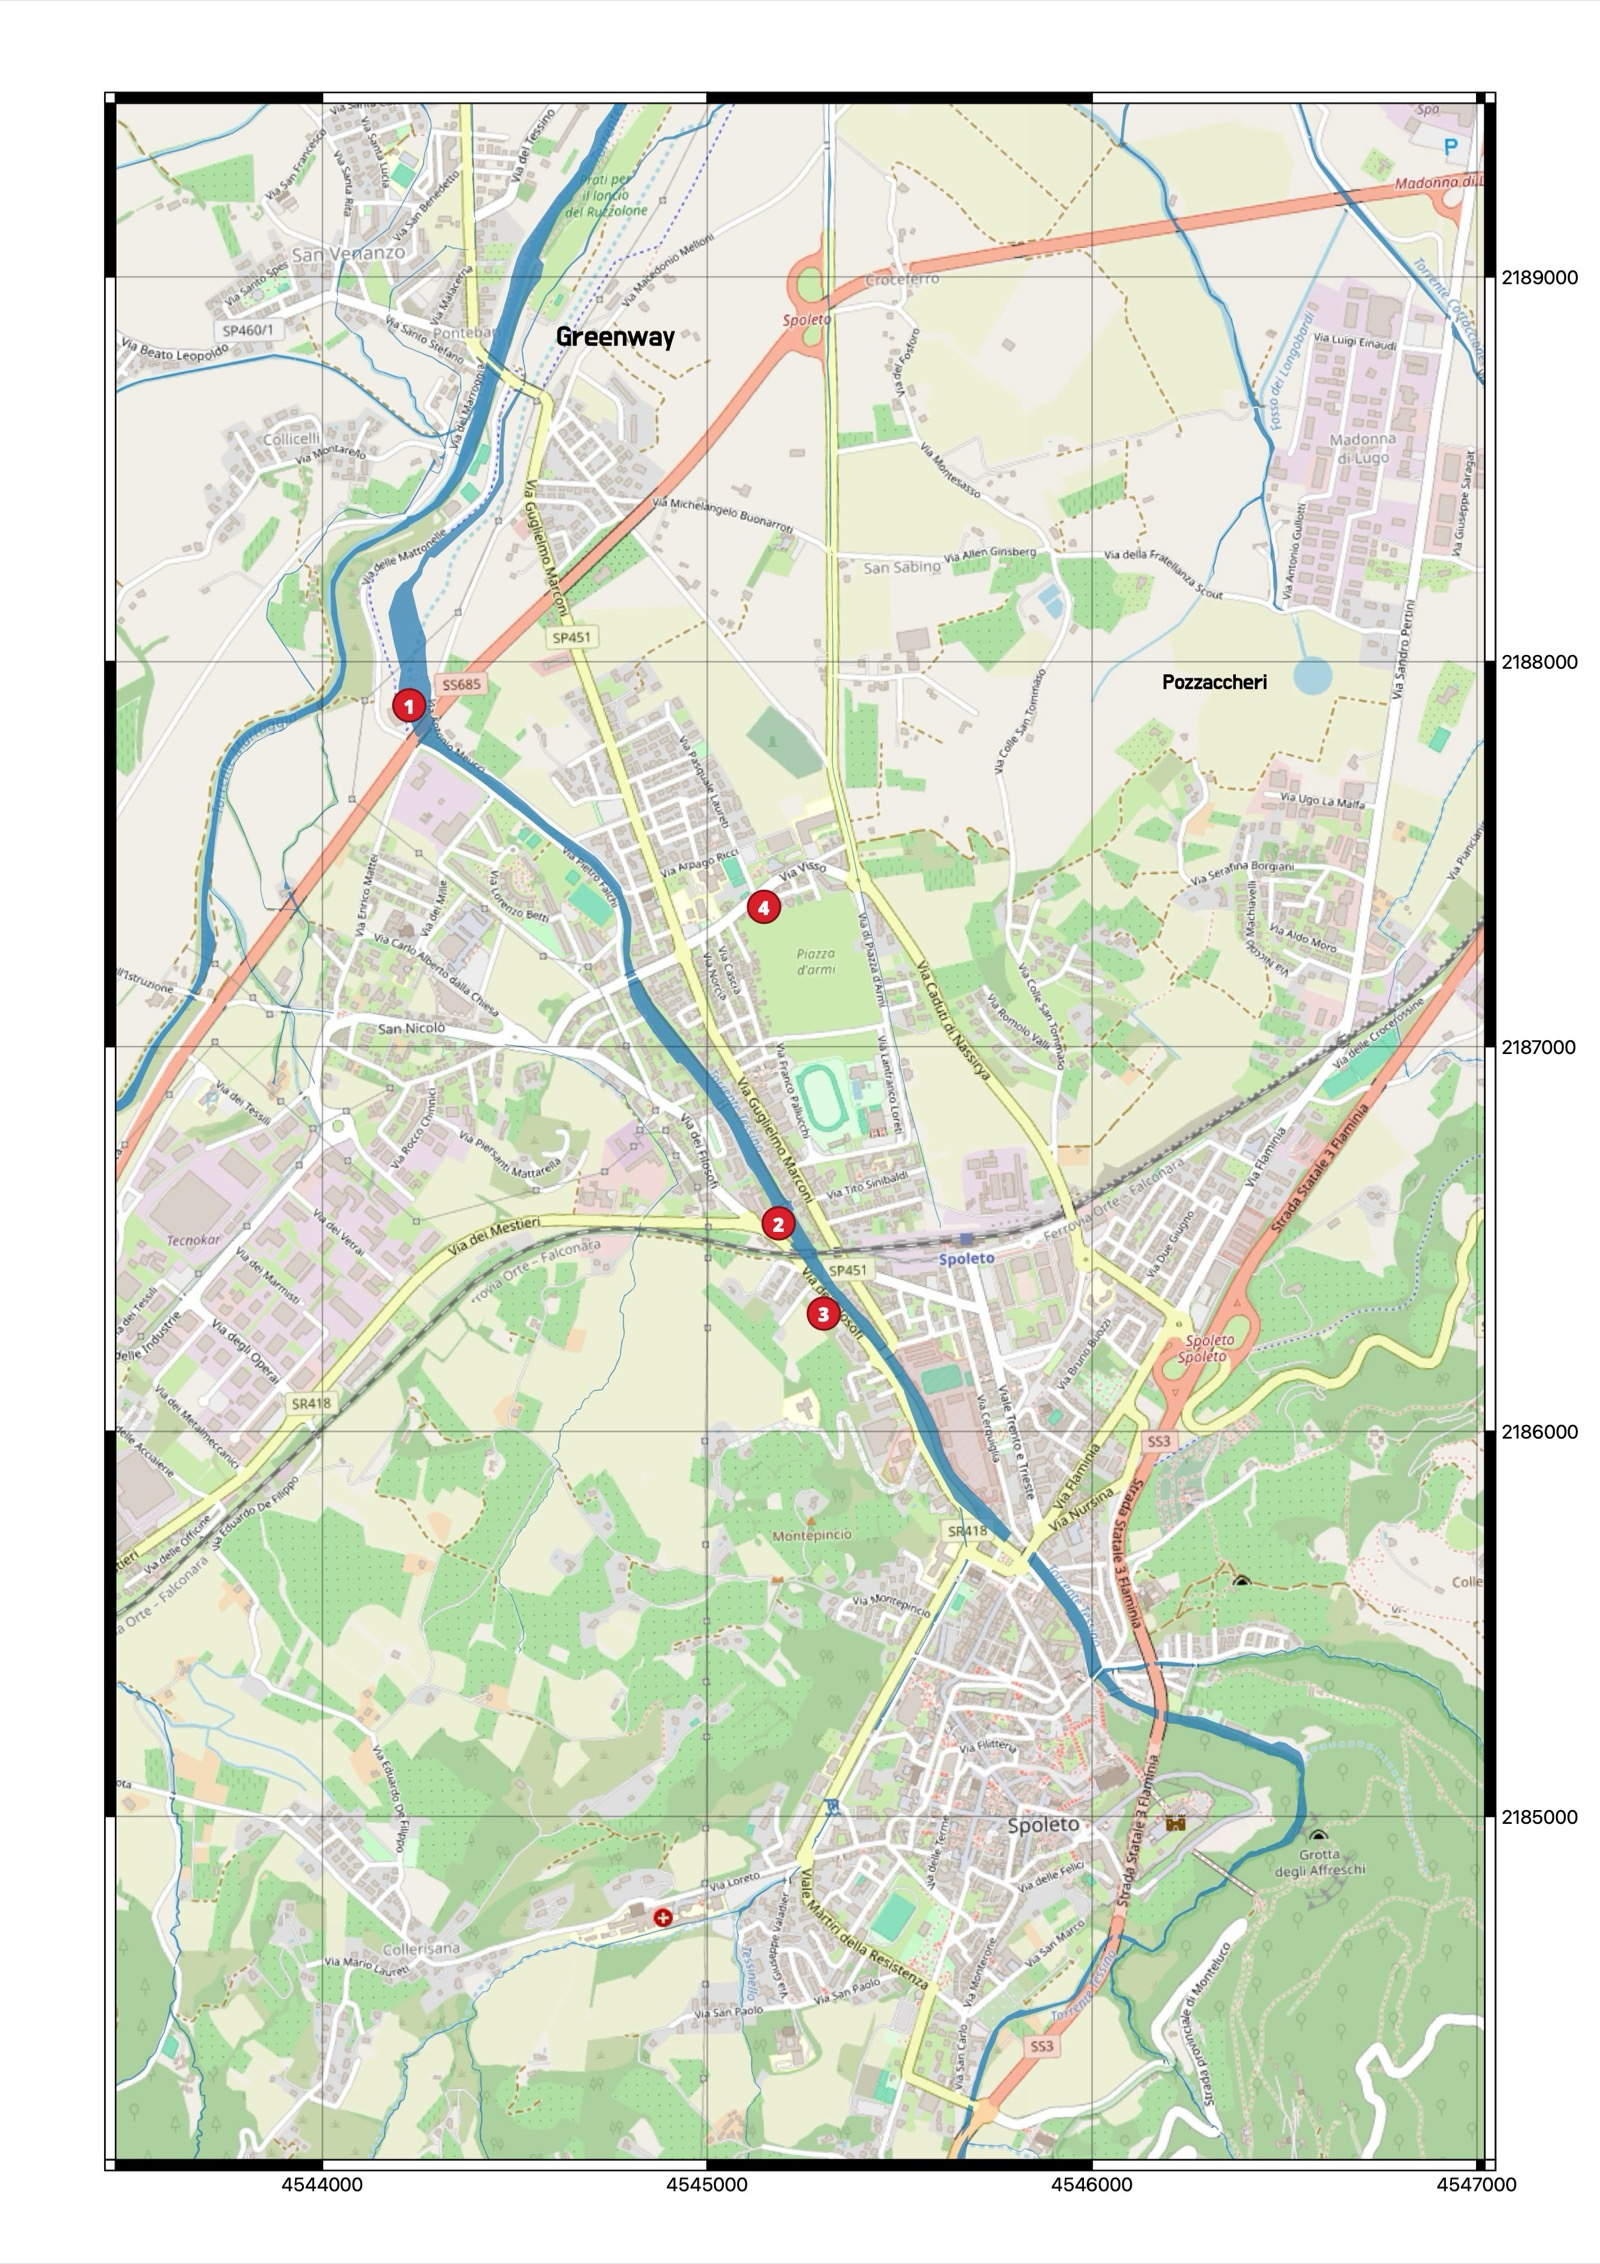
\includegraphics[width=\linewidth,height=\textheight]{./figs/agendaUrbana/Spoleto_AgendaUrbanalifeIMAGINE20250513} 

}

\caption{Mappa di possibile convergenza e sinergia tra le attività in programmazione per Agenda Urbana e con il progetto lifeIMAGINE}\label{fig:agULife}
\end{figure}

\chapter{Disseminazione dei risultati}\label{obs}

Durante lo sviluppo delle attività di progetto ci sono stati anche momenti di disseminazione, finalizzati a condividere i risultati finora raggiunti e a promuoverne la diffusione presso le scuole, la comunità cittadina, i decisori politici e gli stakeholder territoriali. L'obiettivo è stato quello di contribuire a un dibattito aperto sulle questioni legate alla frammentazione territoriale e all'importanza della conservazione della biodiversità per sé e per lo sviluppo di un territorio che possa offrire servizi ecosistemici per il benessere dei cittadini.

Le attività di disseminazione sono state articolate attraverso diverse modalità comunicative (lezioni, presentazioni a convegni e incontri pubblici), al fine di raggiungere target differenziati e assicurare un'ampia diffusione dei contenuti.

Una particolare attenzione verrà rivolta soprattutto durante la fine del 2025 alle azioni di sensibilizzazione per la messa a sistema di forme di scienza partecipata in tutto il territorio comunale. La citizen science rappresenta infatti, una rivoluzione nel modo di concepire la ricerca scientifica, trasformando i cittadini comuni in collaboratori attivi nella raccolta e, attraverso un'adeguata informazione, anche di analisi dei dati. Attraverso piattaforme digitali intuitive, milioni di persone nel mondo contribuiscono quotidianamente a progetti di ricerca che spaziano dalla biodiversità alla salute pubblica. Il potenziale di raccolta dati di questi strumenti è straordinario. Progetti come Observation.org o iNaturalist, molto utili per la catalogazione della flora e fauna, hanno già raccolto milioni di osservazioni, creando database di dimensioni e granularità impossibili da mettere in campo con metodi tradizionali. La capillarità territoriale dei cittadini-scienziati permetterebbe anche ai gestiori del territorio di monitorare fenomeni su scala globale con una densità spaziale e temporale senza precedenti.
Tanto per fornire un quadro iniziale della situazione specifica relativa al comune di Spoleto si possono osservare le segnalazioni che sono già pervenute all'interno della piattaforma europea Observation.org, senza che ci siano state intense campagne informative e promozionali locali (Fig. \ref{fig:obs2025}).

\begin{figure}

{\centering 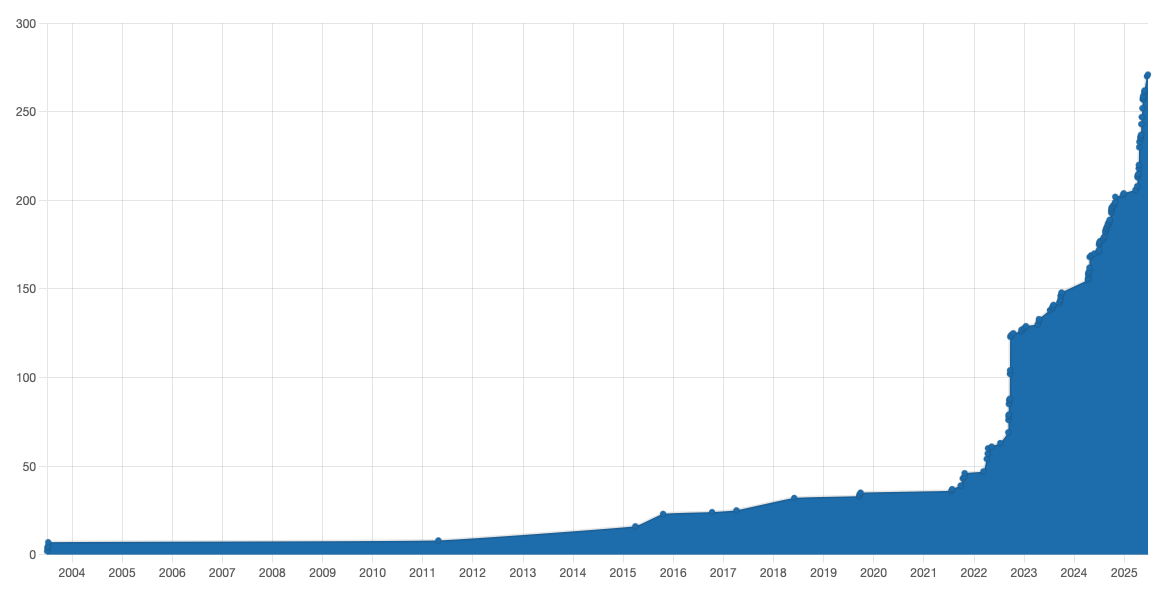
\includegraphics[width=\linewidth]{./figs/observationPlot} 

}

\caption{Trend delle segnalazioni naturalistiche pervenute all'interno della piattaforma di scienza partecipata [Observation.org](https://observation.org) (giugno 2025)}\label{fig:obs2025}
\end{figure}

Molteplici e profondi sono i benefici per la comunità. A livello educativo, la partecipazione diretta alla ricerca aumenta la consapevolezza ambientale dei cittadini. Sul piano sociale, questi progetti creano reti di collaborazione che rafforzano il senso di appartenenza e responsabilità collettiva verso i beni comuni. Come evidenziato nel grafico siamo nel pieno del processo di crescita di questo fenomeno e restare indietro senza coglierne apppieno le potenzialità si rivelerebbe un'occasione persa per costruire una società più informata e scientificamente consapevole.

\section{Eventi di disseminazione}\label{eventi-di-disseminazione}

Di seguito vengono elencati i principali eventi su scala locale in cui sono stati illustrati i risultati del progetto, le metodologie sviluppate e applicate e i prodotti cartografici realizzati:

\begin{itemize}
\tightlist
\item
  attività PCTO, ovvero Percorsi per le Competenze Trasversali e l'Orientamento, con le scuole secondarie di secondo ordine (Istituto Tecnico Agrario della Valnerina di S. Anatolia di Narco, Istituto Tecnico e Professionale ``Spagna - Campani'' e Liceo Scientifico ``Sansi Leonardi Volta'' di Spoleto) presso il Punto digitale Facile - Digipass di Spoleto
\item
  Convegno Fauna2024 - con un contributo dal titolo ``Fauna in campagna: biodiversità e paesaggio rurale''
\item
  Museo delle Scienze e del Territorio MUST di Spoleto - con un intervento sul tema ``Diventare un citizen scientist per il monitoraggio della fauna minore''
\item
  Convegno Fauna2025 - con un contributo dal titolo ``Reti Ecologiche e Natura 2000: pianificazione e conservazione''
\end{itemize}

In \hyperref[annexI]{Allegato I} si riportano le diapositive delle presentazioni utilizzate durante questi momenti di condivisione e disseminazione.

\chapter{Considerazioni conclusive}\label{considerazioni-conclusive}

Le proiezioni demografiche indicano che nei prossimi decenni oltre il 65\% della popolazione mondiale risiederà e lavorerà in contesti urbani (==BIB==). Benché la diversità specifica nelle città risulti generalmente ridotta rispetto agli habitat naturali, è stata documentata la presenza di un numero considerevole di specie (==BIB==). In alcuni casi, gli ambienti urbani possono addirittura offrire rifugio anche a specie che sono valutate ad elevato rischio rischio di estinzione secondo i criteri dell'Unione Internazionale per la Conservazione della Natura (IUCN). Una recente meta-analisi condotta su un ampio dataset ha evidenziato infatti come l'estensione complessiva delle aree verdi urbane, unitamente alla presenza di corridoi ecologici e a una struttura del verde articolata, costituisca un fattore determinante per la ricchezza specifica locale (==BIB==).

In questo contesto di crescente urbanizzazione globale, anche il territorio spoletino assume un valore strategico particolare. Il quadro faunistico tracciato nella presente relazione evidenzia infatti l'elevato valore naturalistico di quest'area che richiede dunque un approccio gestionale equilibrato tra conservazione delle specie già note e promozione di ricerche per colmare le lacune conoscitive, specialmente nel mondo degli invertebrati che potrebbero riservare importanti sorprese dal punto di vista della biodiversità. La presenza di 113 specie tutelate dalla Direttiva Habitat (circa il 21\% del totale) rafforza l'importanza dell'area e la necessità di proseguire nelle azioni di tutela e mantenimento dello stato del territorio attraverso strategie di conservazione oculate anche al di fuori delle aree Natura 2000. Gli uccelli e i mammiferi, essendo meglio conosciuti, possono costituire la base per immediate strategie di tutela, mentre per gli invertebrati serve un approccio prudenziale da valutare caso per caso.

L'incorporazione delle reti ecologiche nella pianificazione municipale rappresenta un elemento strategico per assicurare uno sviluppo territoriale sostenibile, salvaguardando la biodiversità e rafforzando la resilienza ecosistemica. Per soddisfare in primo luogo il benessere dei propri cittadini le politiche territoriali e urbanistiche locali hanno il dovere di considerare l'interconnessione tra ambiti naturali e antropizzati, realizzando infrastrutture verdi e corridoi ecologici che supportino la fauna e la flora autoctone in un'ottica di quella multifunzionalità che garantisce simultaneamente servizi ecosistemici essenziali, qualità ambientale urbana e opportunità ricreative per la comunità locale (cfr. ==Fairbairn et al., 2024==).

Il territorio spoletino attualmente presenta una pressione insediativa relativamente contenuta con meno del 6\% ascrivibile ad area urbana in senso stretto. Anche la ripartizione tra aree boscate (46\%) e aree agricole (circa 31\% tra seminativi e oliveti) evidenzia un territorio che mantiene un buon equilibrio tra componenti naturali e attività umane tradizionali. Tuttavia, le analisi dei pattern spaziali danno conto della presenza di numerose tessere di piccole dimensioni, con processi di frammentazione in corso che costituiscono una minaccia per la continuità ecologica. Il basso indice di coesione (mediamente 9.56 su 100) segnala un certo grado di disconnessione tra le diverse componenti del paesaggio, con potenziali impatti negativi sulla biodiversità e sui servizi ecosistemici. La chiave di lettura principale è che ci troviamo davanti a un territorio che ha ancora le potenzialità per mantenere un equilibrio sostenibile, ma che richiede una serie di interventi diretti mirati a mantenere e migliorare le connessioni ecologiche, cruciali per garantire un buono stato di conservazione del sistema paesaggistico-ecologico.

In linea generale, gli strumenti di pianificazione e zonizzazione ecologica, quali i piani urbanistici e le normative sull'uso del suolo, hanno un ruolo determinante nella definizione di aree protette, corridoi verdi e zone di compensazione ambientale. Tali strumenti consentono di integrare la conservazione della natura nelle dinamiche urbane, mitigando l'impatto delle infrastrutture sul paesaggio naturale.

Grazie all'analisi dei pattern morfologici è stato possibile mettere in luce un chiara differenza nella struttura dell'habitat tra il territorio comunale nella sua interezza e quello della fascia collinare, rivelando l'importanza critica di quest'area a vocazione più produttiva. In una prospettiva generale il territorio si presenta con una struttura ecologica potenzialmente di buon livello, dominata da ampie aree Core (70.8\%) con elevata connettività interna (Effective mesh size) e frammentazione limitata (Splitting Index: 6.88). Questo scenario configura un sistema ecologico robusto, dove i corridoi naturali e i ponti ecologici, seppur rappresentando percentuali modeste del territorio, svolgono ancora la loro funzione di collegamento. Il piano collinare rivela invece una realtà diversa: le aree Core si riducono drasticamente al 38.8\% con un crollo dell'Effective mesh size e un incremento significativo della frammentazione (Splitting Index: 157.79). Particolarmente preoccupante è l'espansione delle aree Edge al 19.5\%, che segnala una maggiore vulnerabilità degli habitat alle pressioni esterne. Allo stesso modo numerosi sono gli elementi di connessione interrotti (Pattern 1/101), presenti con oltre 2000 patches nell'8.1\% del territorio collinare, indicando la necessità di una pianificazione di una rete ecologica con interventi mirati soprattutto al ripristino della connettività. A dare conforto, la concentrazione delle Islet in clusters piuttosto che in frammenti completamente dispersi. Questa particolare configurazione offre opportunità concrete per strategie di riconnessione volte al potenziamento di stepping stones e dei corridoi verdi e blu, in primis l'area della greenway lungo il torrente Tessino e l'intero sistema delle aree umide.

In conclusione, l'analisi condotta conferma che il territorio esaminato si caratterizza come un paesaggio dinamico che mantiene un patrimonio forestale di grande valore e presenta numerose aree con significativo potenziale di connettività ecologica. Per valorizzare appieno queste risorse naturali è necessaria una stretta collaborazione tra amministrazione comunale e cittadinanza, finalizzata a costruire una visione condivisa del futuro territoriale e a realizzare progetti concreti di sviluppo sostenibile.

\chapter{Programmazione 2025}\label{programmazione-2025}

\section{Piano delle attività 2025}\label{piano-delle-attivituxe0-2025}

Il panel di obiettivi definiti per il 2025 ha lo scopo di proseguire lo
studio dei pattern del territorio e della biodiversità che lo
caratterizzano. Ciò è finalizzato a fornire elementi di valutazione
scientificamente solidi per lo sviluppo della rete ecologica comunale e
conseguentemente a: i) supportare la biodiversità locale e ii)
migliorare la qualità ambientale urbana e periurbana.

In particolare gli aspetti su cui verrà focalizzata l'attenzione
saranno:

\begin{itemize}
\item
  \textbf{Prosecuzione delle analisi dei Pattern Morfologici e
  Prioritizzazione degli Interventi}. Tale attività prevede la
  mappatura e lo studio di approfondimento delle caratteristiche
  morfologiche del territorio per identificare le aree strategiche per
  la creazione di corridoi ecologici. Questa analisi permetterà di
  suggerire una gerarchia di interventi basata su criteri di urgenza
  ecologica, fattibilità tecnica e impatto ambientale.
\item
  \textbf{Valutazione degli Indicatori Ecologici}. Per questo obiettivo
  saranno indagati gli indicatori specifici per misurare e monitorare
  l'efficacia degli interventi di connettività ecologica, includendo
  parametri di biodiversità, qualità degli habitat e funzionalità
  ecosistemica.
\item
  \textbf{Supporto agli Interventi dell'Agenda Urbana}. Questa attività di
  supporto tecnico potrà essere funzionale per l'implementazione degli
  interventi previsti da Agenda Urbana, garantendo l'integrazione
  degli obiettivi di sostenibilità ambientale e di tutela delle
  biodiversità nelle politiche di sviluppo territoriale, anche tenendo
  conto delle componenti a invertebrati.
\item
  \textbf{Collaborazione ponte con il Progetto LIFE IMAGINE}. Questa azione
  garantirà il supporto operativo per le attività integrative previste
  dal progetto LIFE IMAGINE (LIFE19 IPE/IT/000015) coordinato da
  Regione Umbria, contribuendo al raggiungimento degli obiettivi di
  conservazione e miglioramento degli ecosistemi urbani e periurbani
  municipali.
\item
  \textbf{Sviluppo di un Abaco degli Interventi}. Consisterà nella
  progettazione di un repertorio tecnico standardizzato di interventi
  per la definizione di linee guida operative relative alla
  riqualificazione e manutenzione urbana, fornendo indicazioni
  pratiche in linea con gli obiettivi di progettazione e realizzazione
  di infrastrutture verdi e blu.
\item
  \textbf{Prosecuzione della Campagna di Citizen Science per il Monitoraggio
  Faunistico}. Prosecuzione della campagna di sensibilizzazione e
  raccolta dati faunistici attraverso le piattaforme di scienza
  partecipata come ad es. \href{https://observation.org}{Observation.org},
  coinvolgendo la cittadinanza in bioblitz, nel monitoraggio diffuso
  della biodiversità locale e nella creazione di una banca dati
  partecipativa comunale.
\end{itemize}

\chapter{Allegato I}\label{annexI}

\section{Diapositive delle presentazioni utilizzate durante gli eventi di disseminazione dei risultati della ricerca}\label{diapositive-delle-presentazioni-utilizzate-durante-gli-eventi-di-disseminazione-dei-risultati-della-ricerca}

\subsection{Attività PCTO (Percorsi per le Competenze Trasversali e l'Orientamento) su biodiversità e reti ecologiche}\label{attivituxe0-pcto-percorsi-per-le-competenze-trasversali-e-lorientamento-su-biodiversituxe0-e-reti-ecologiche}

\pandocbounded{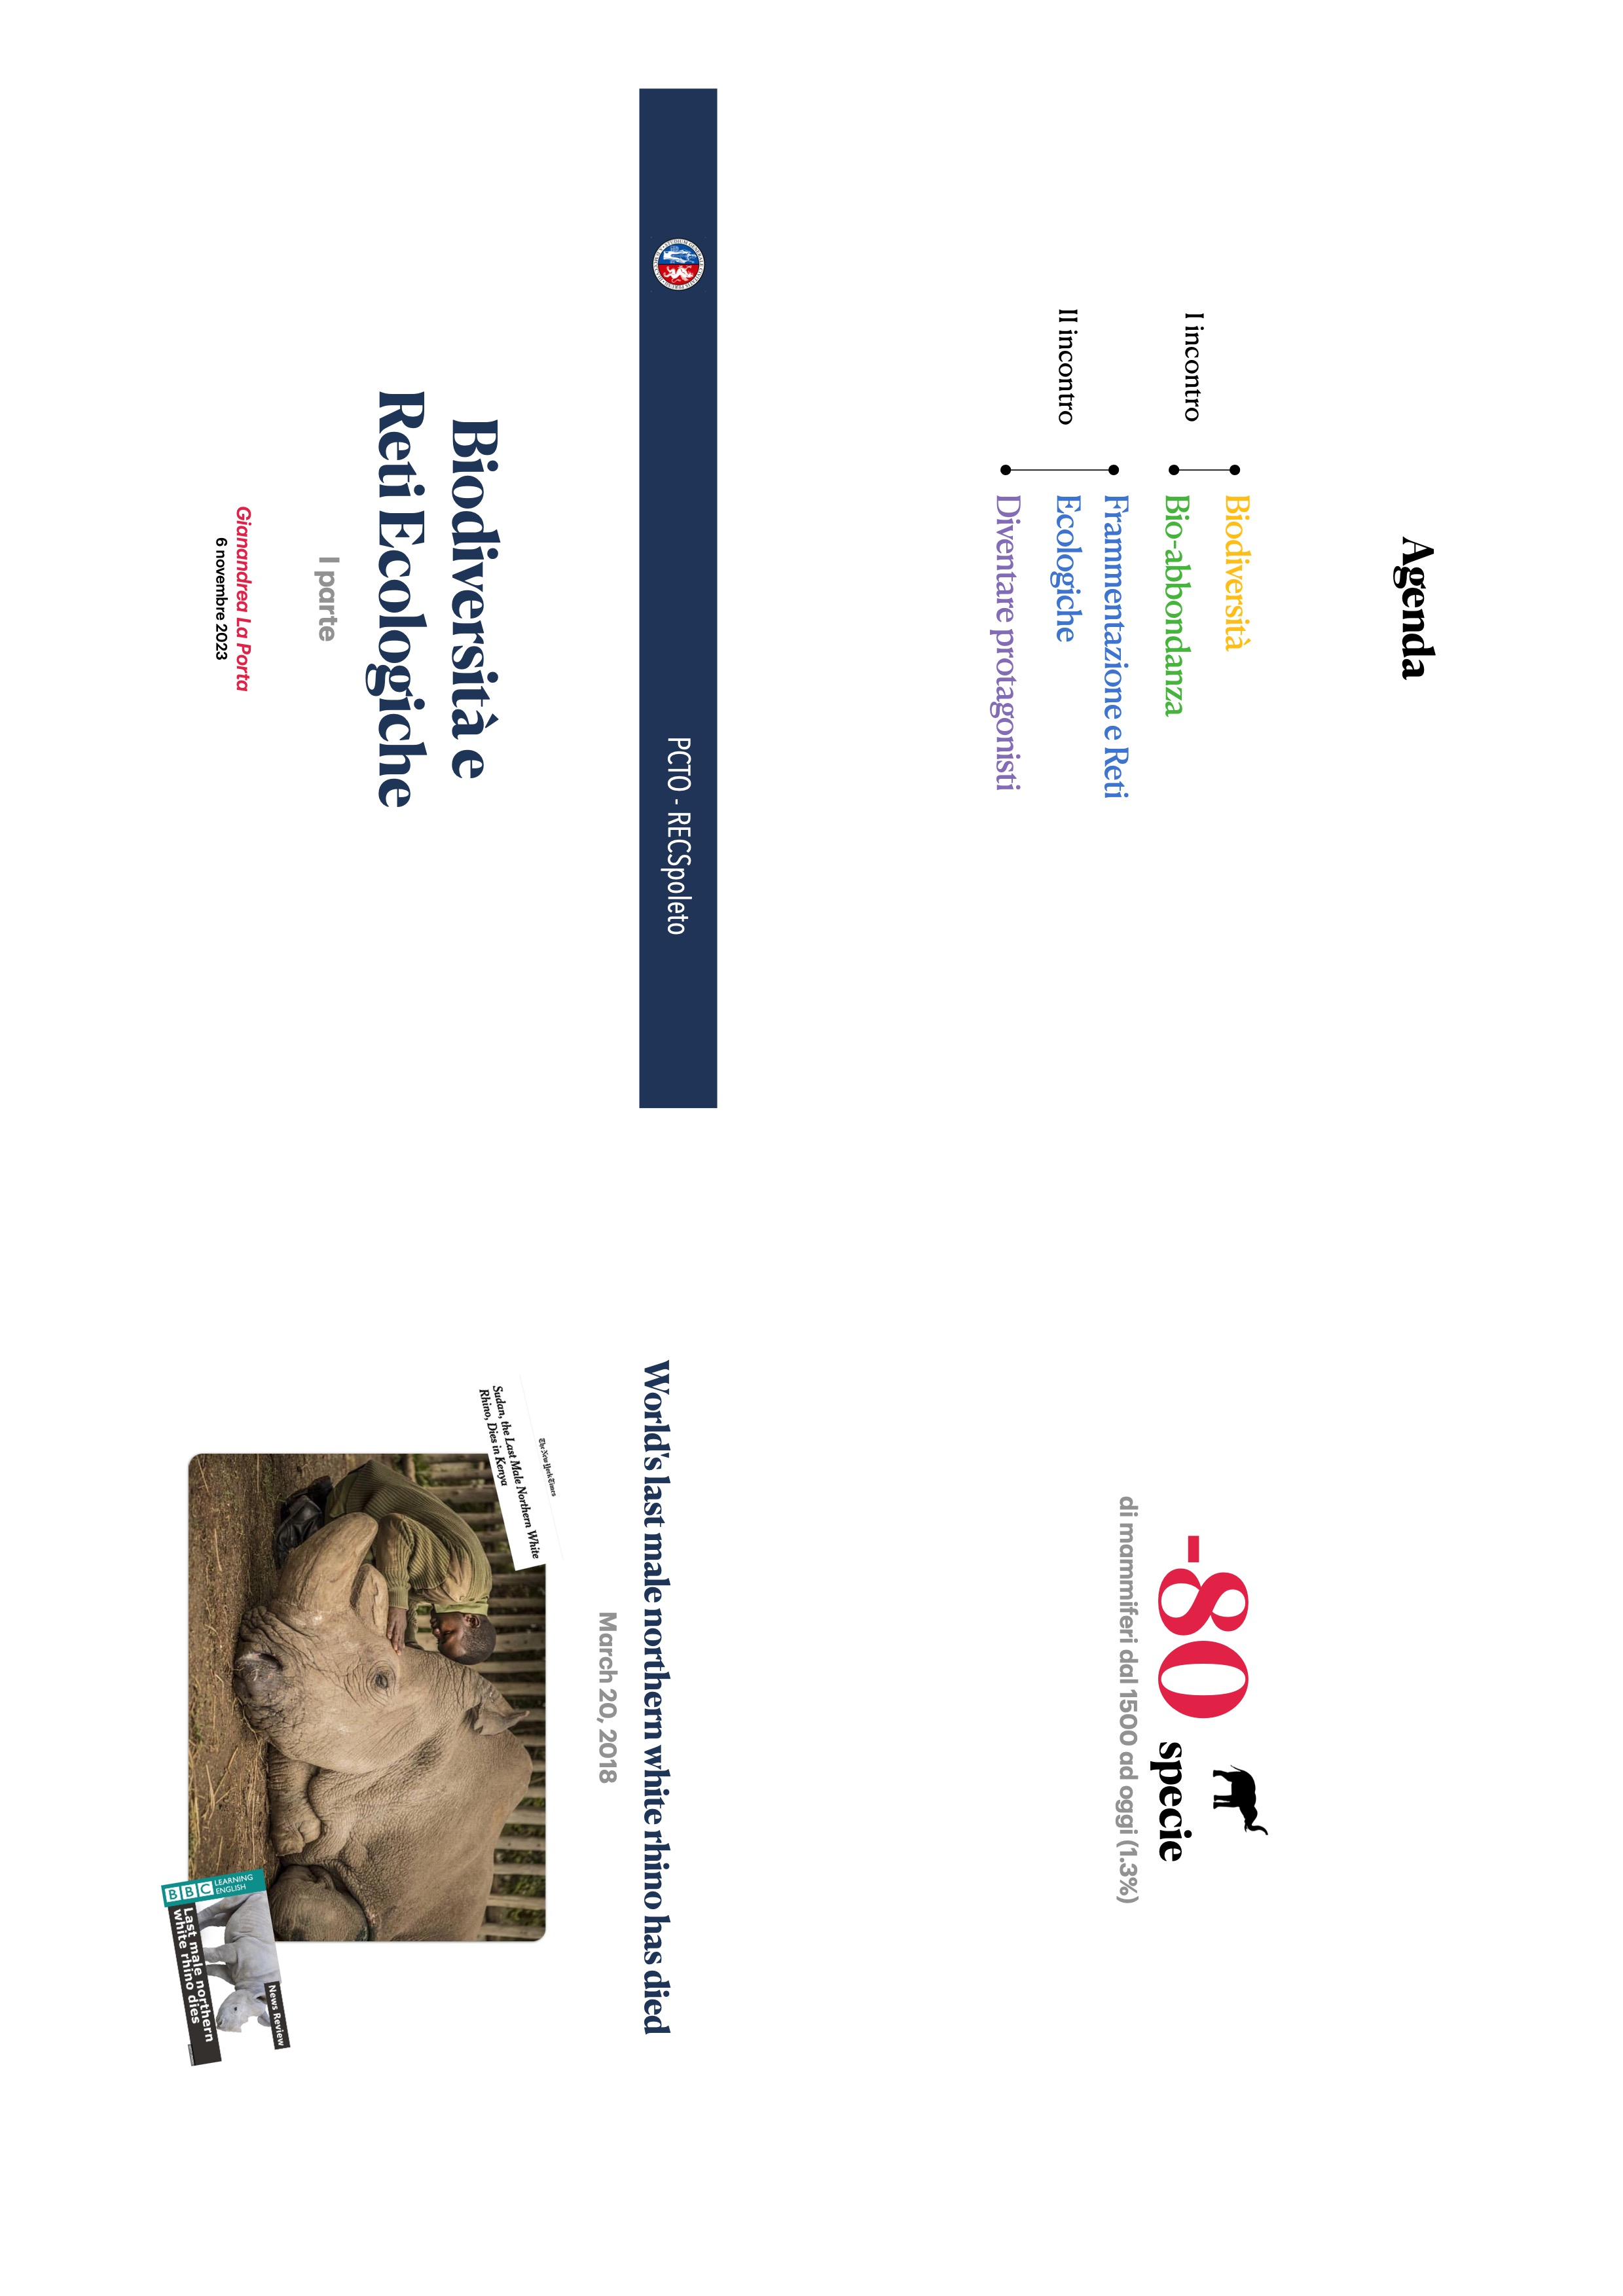
\includegraphics[keepaspectratio]{./figs/pctoREC/diversityRECSpoleto01-1.jpeg}}

\pandocbounded{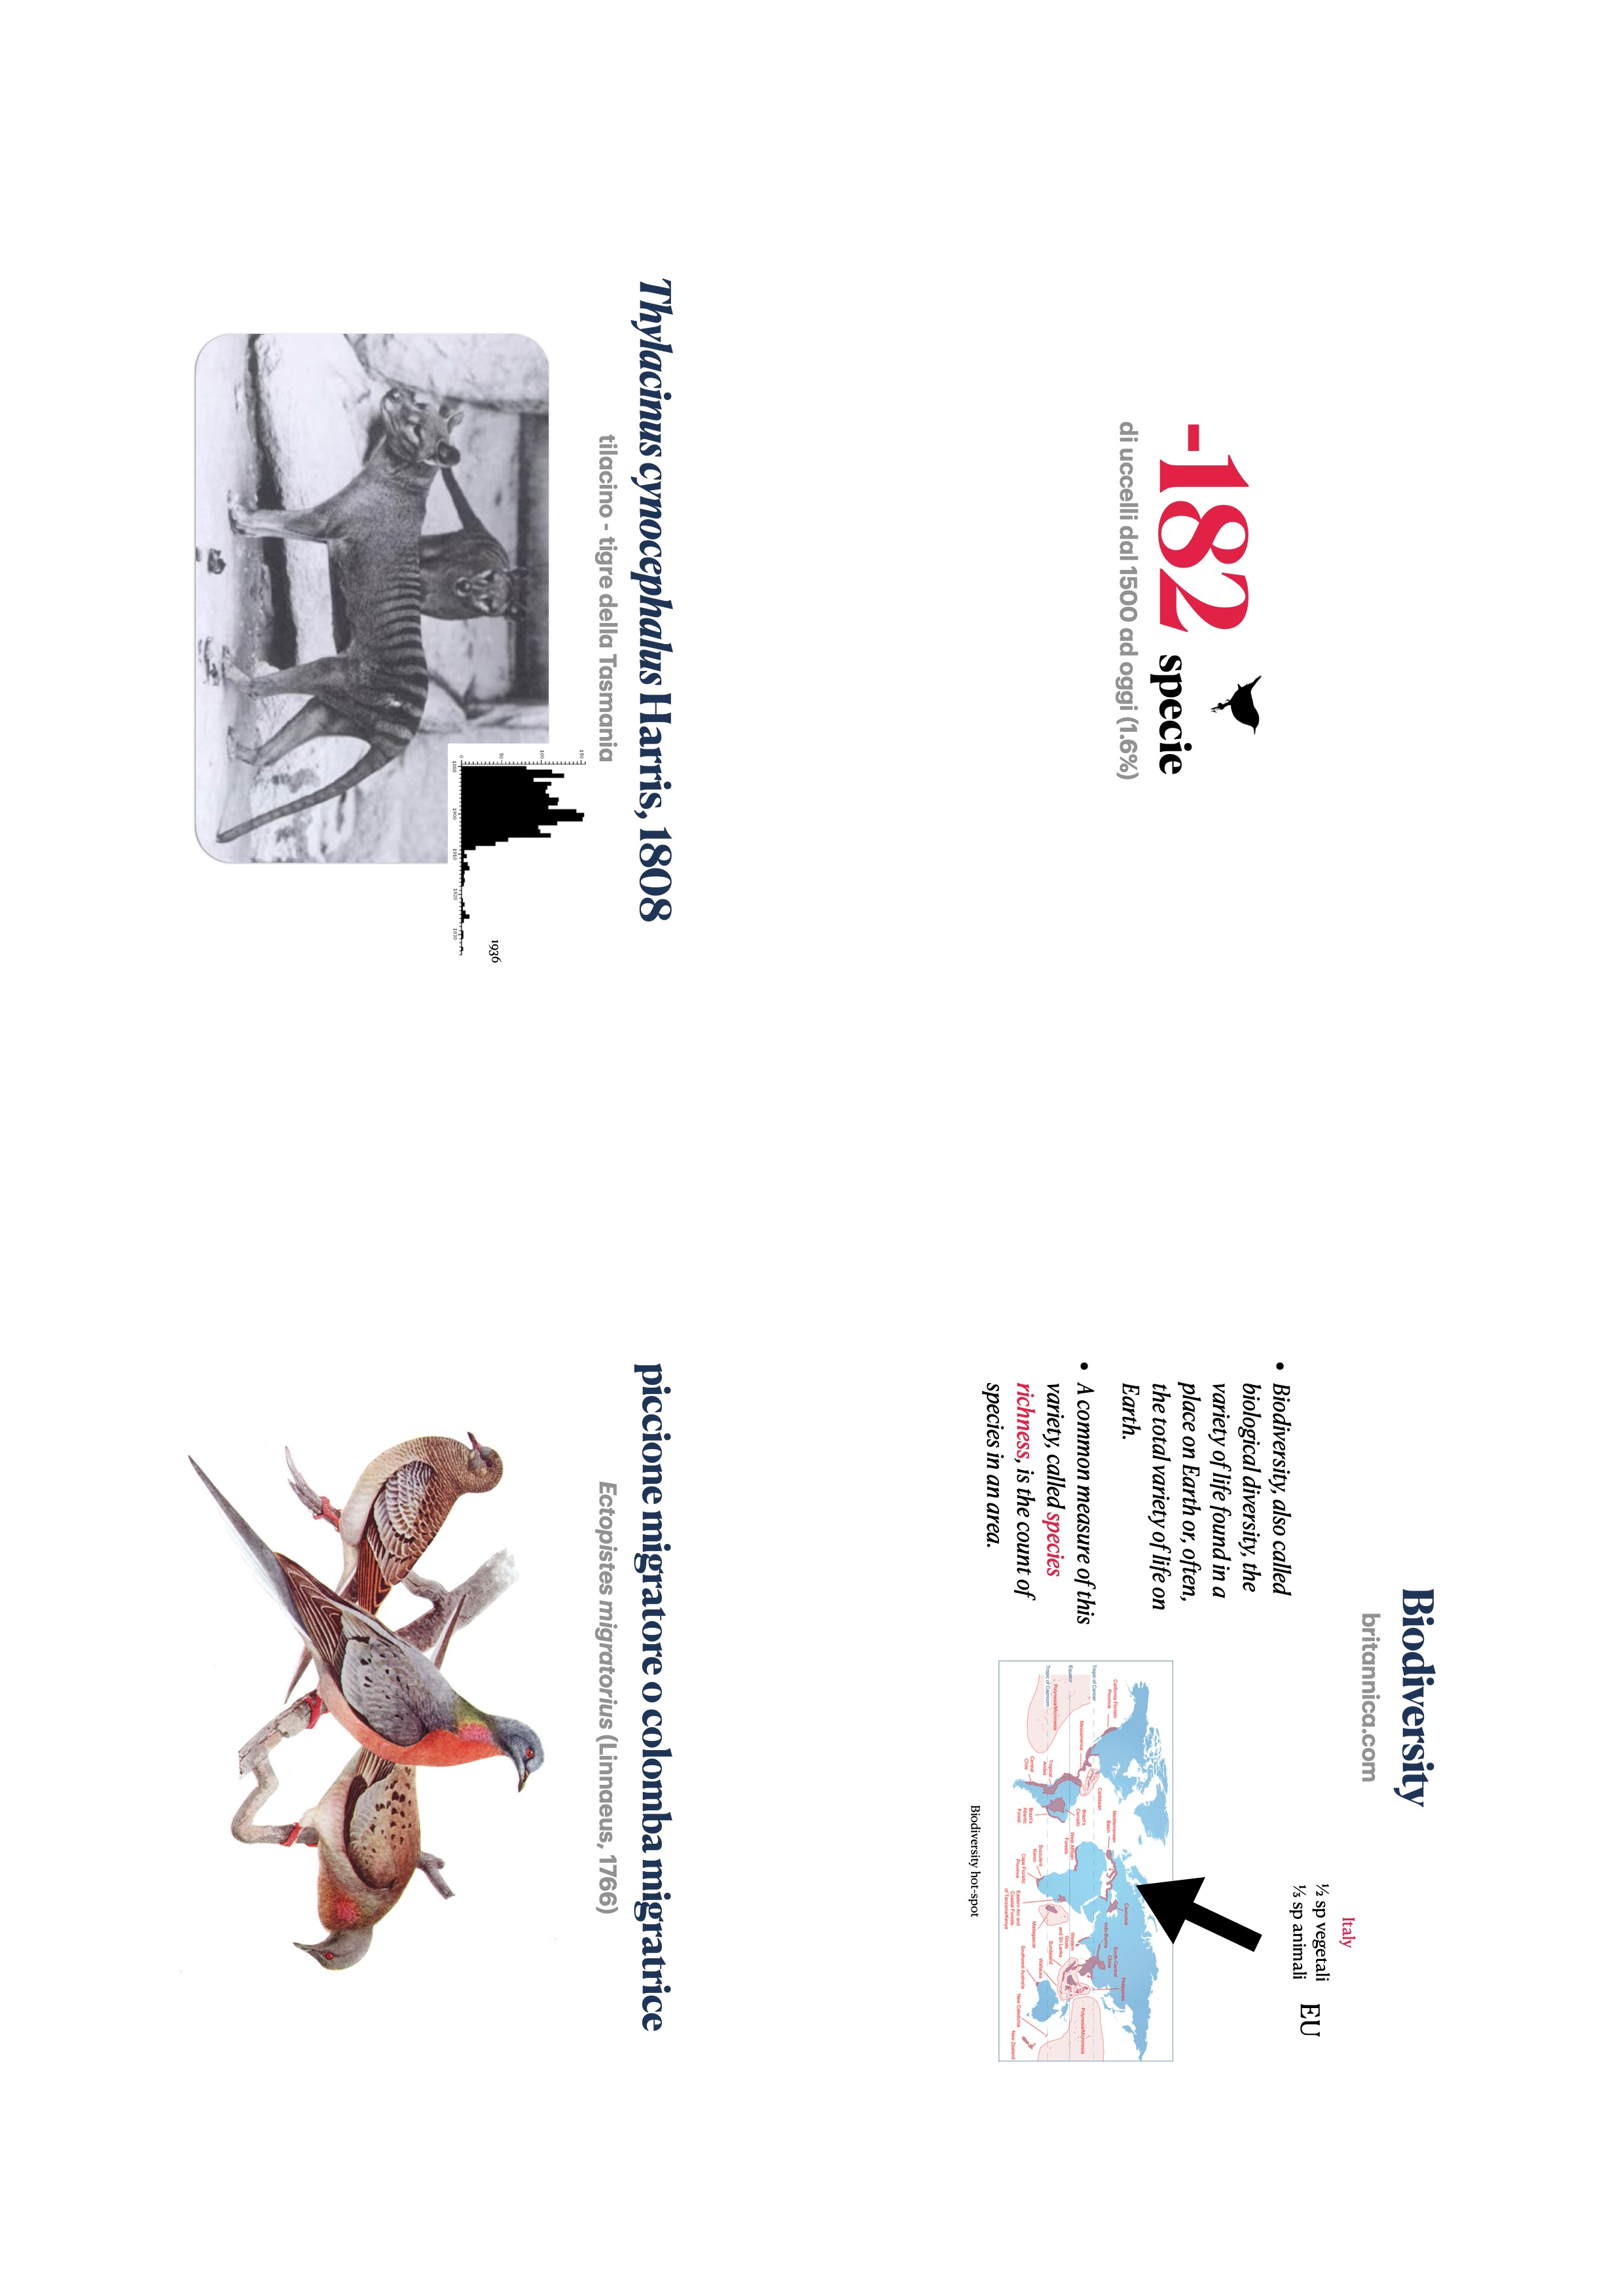
\includegraphics[keepaspectratio]{./figs/pctoREC/diversityRECSpoleto01 2-2.jpeg}}

\pandocbounded{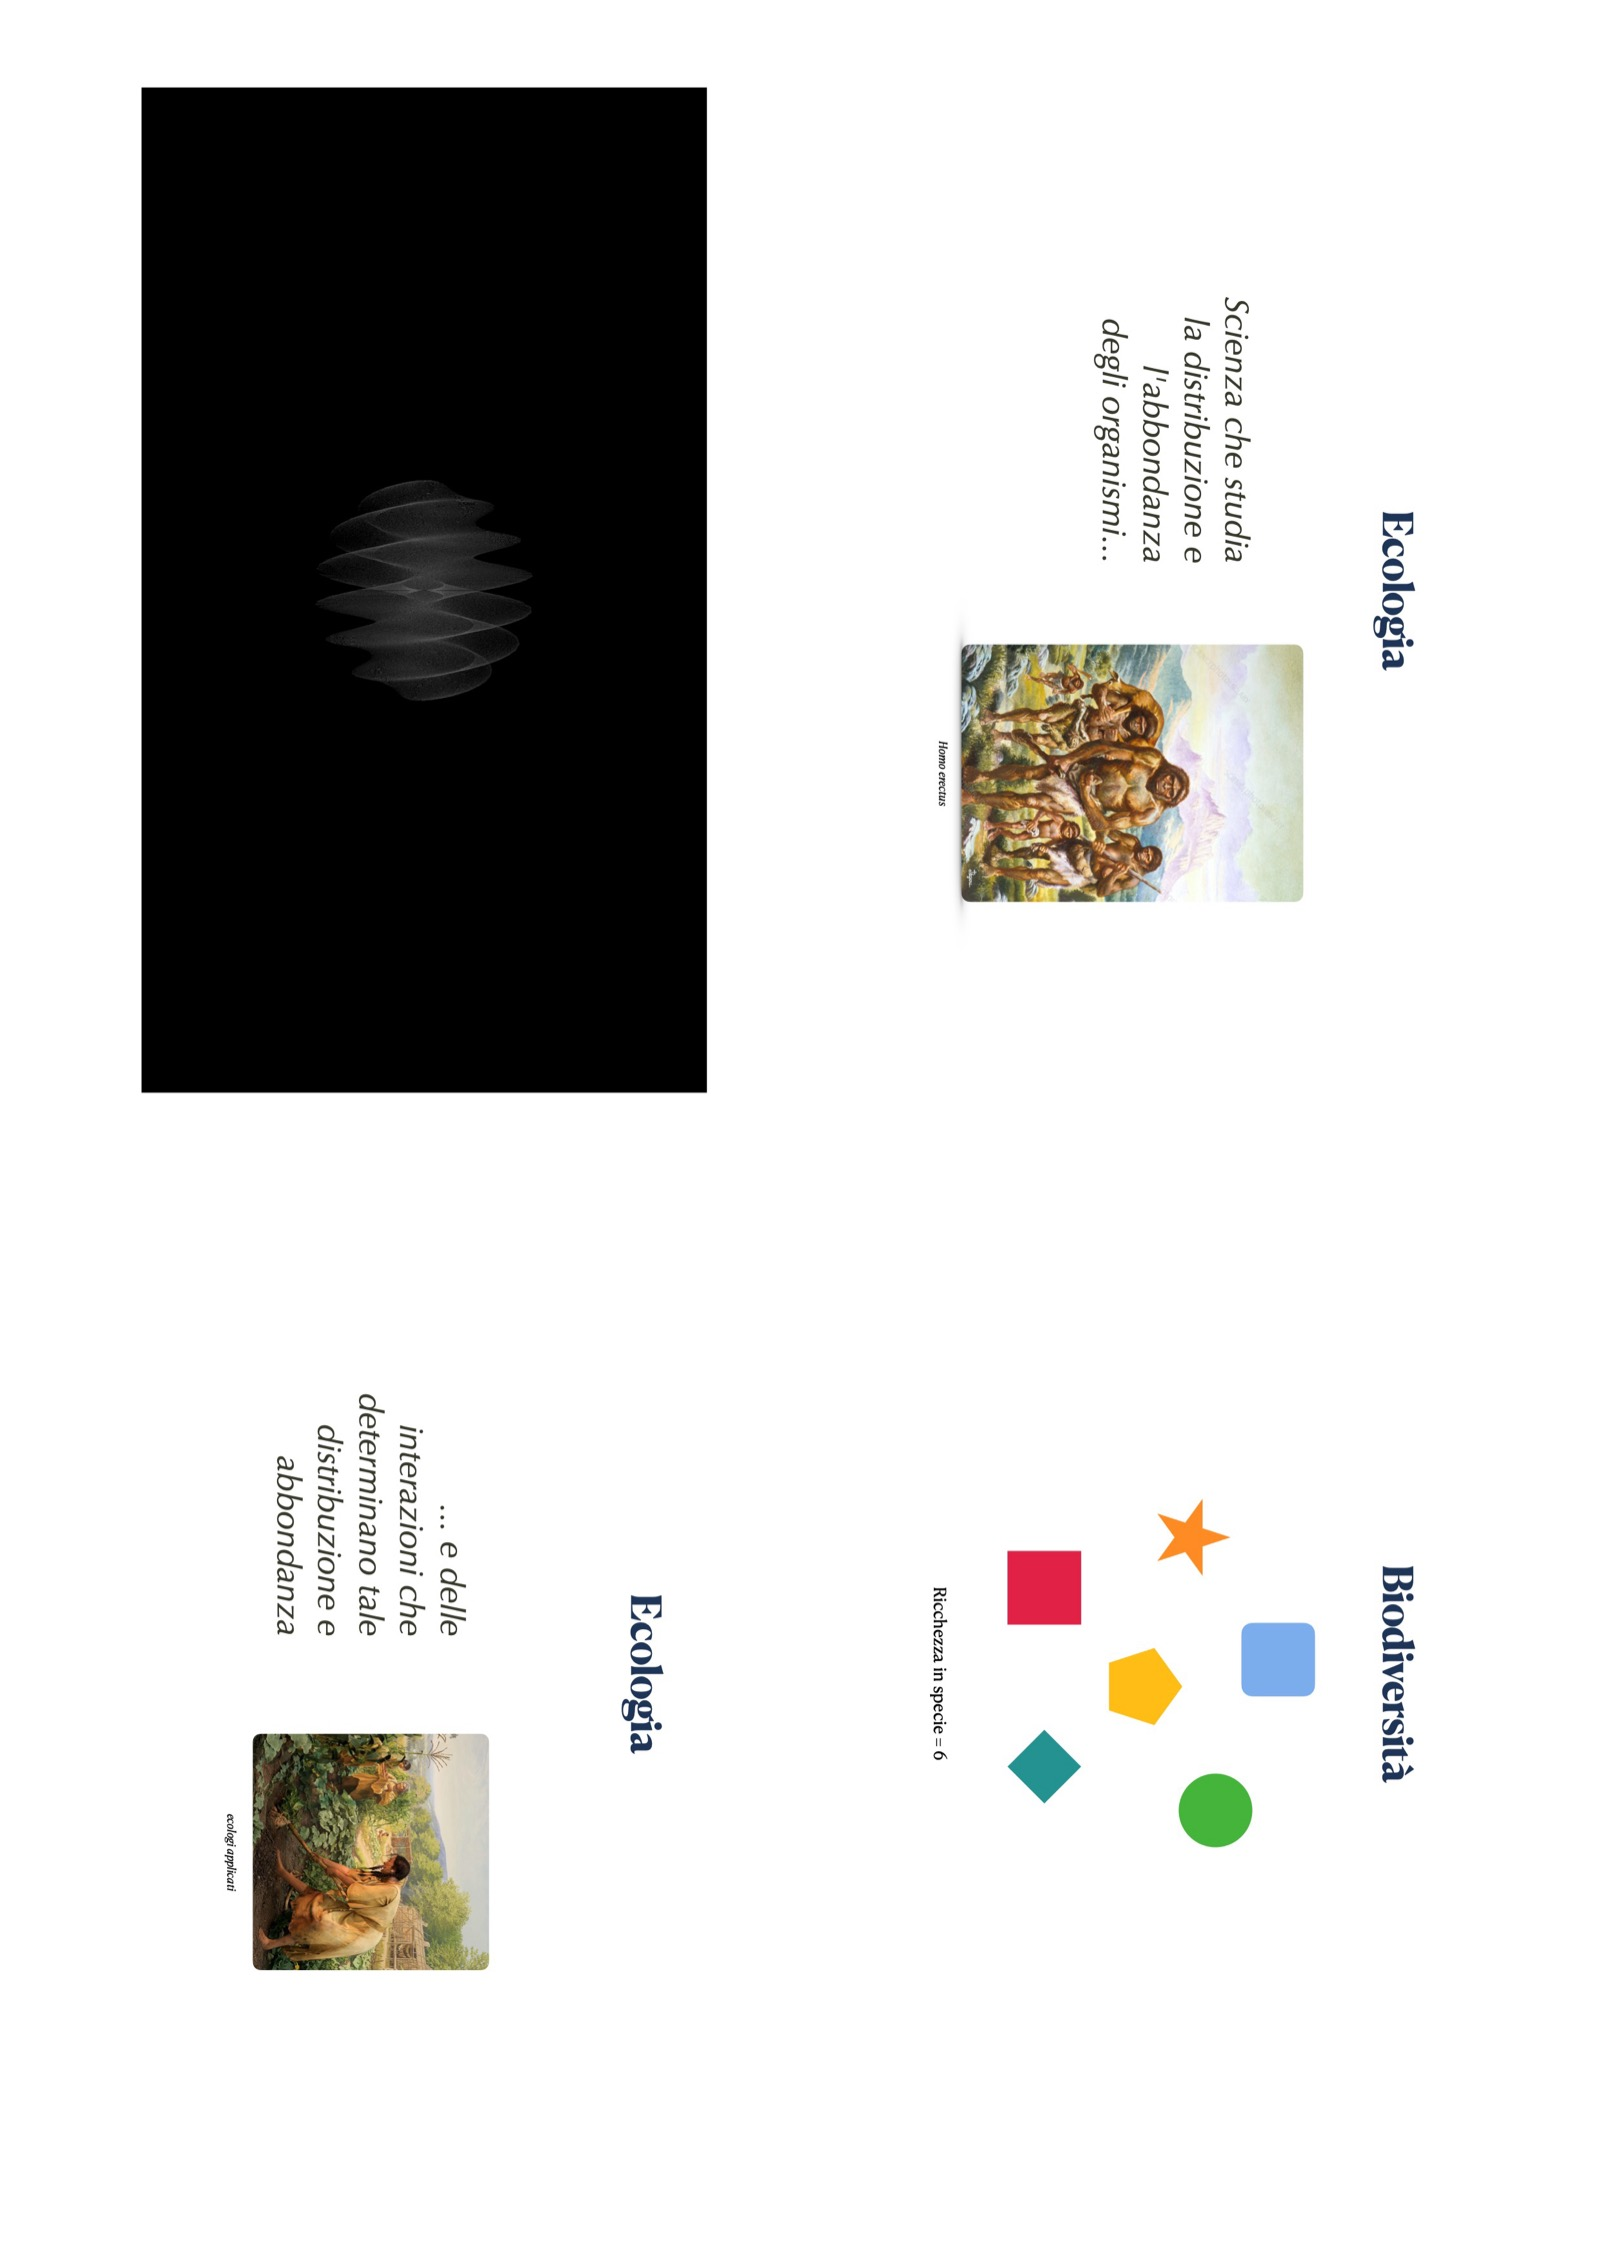
\includegraphics[keepaspectratio]{./figs/pctoREC/diversityRECSpoleto01 3-3.jpeg}}

\pandocbounded{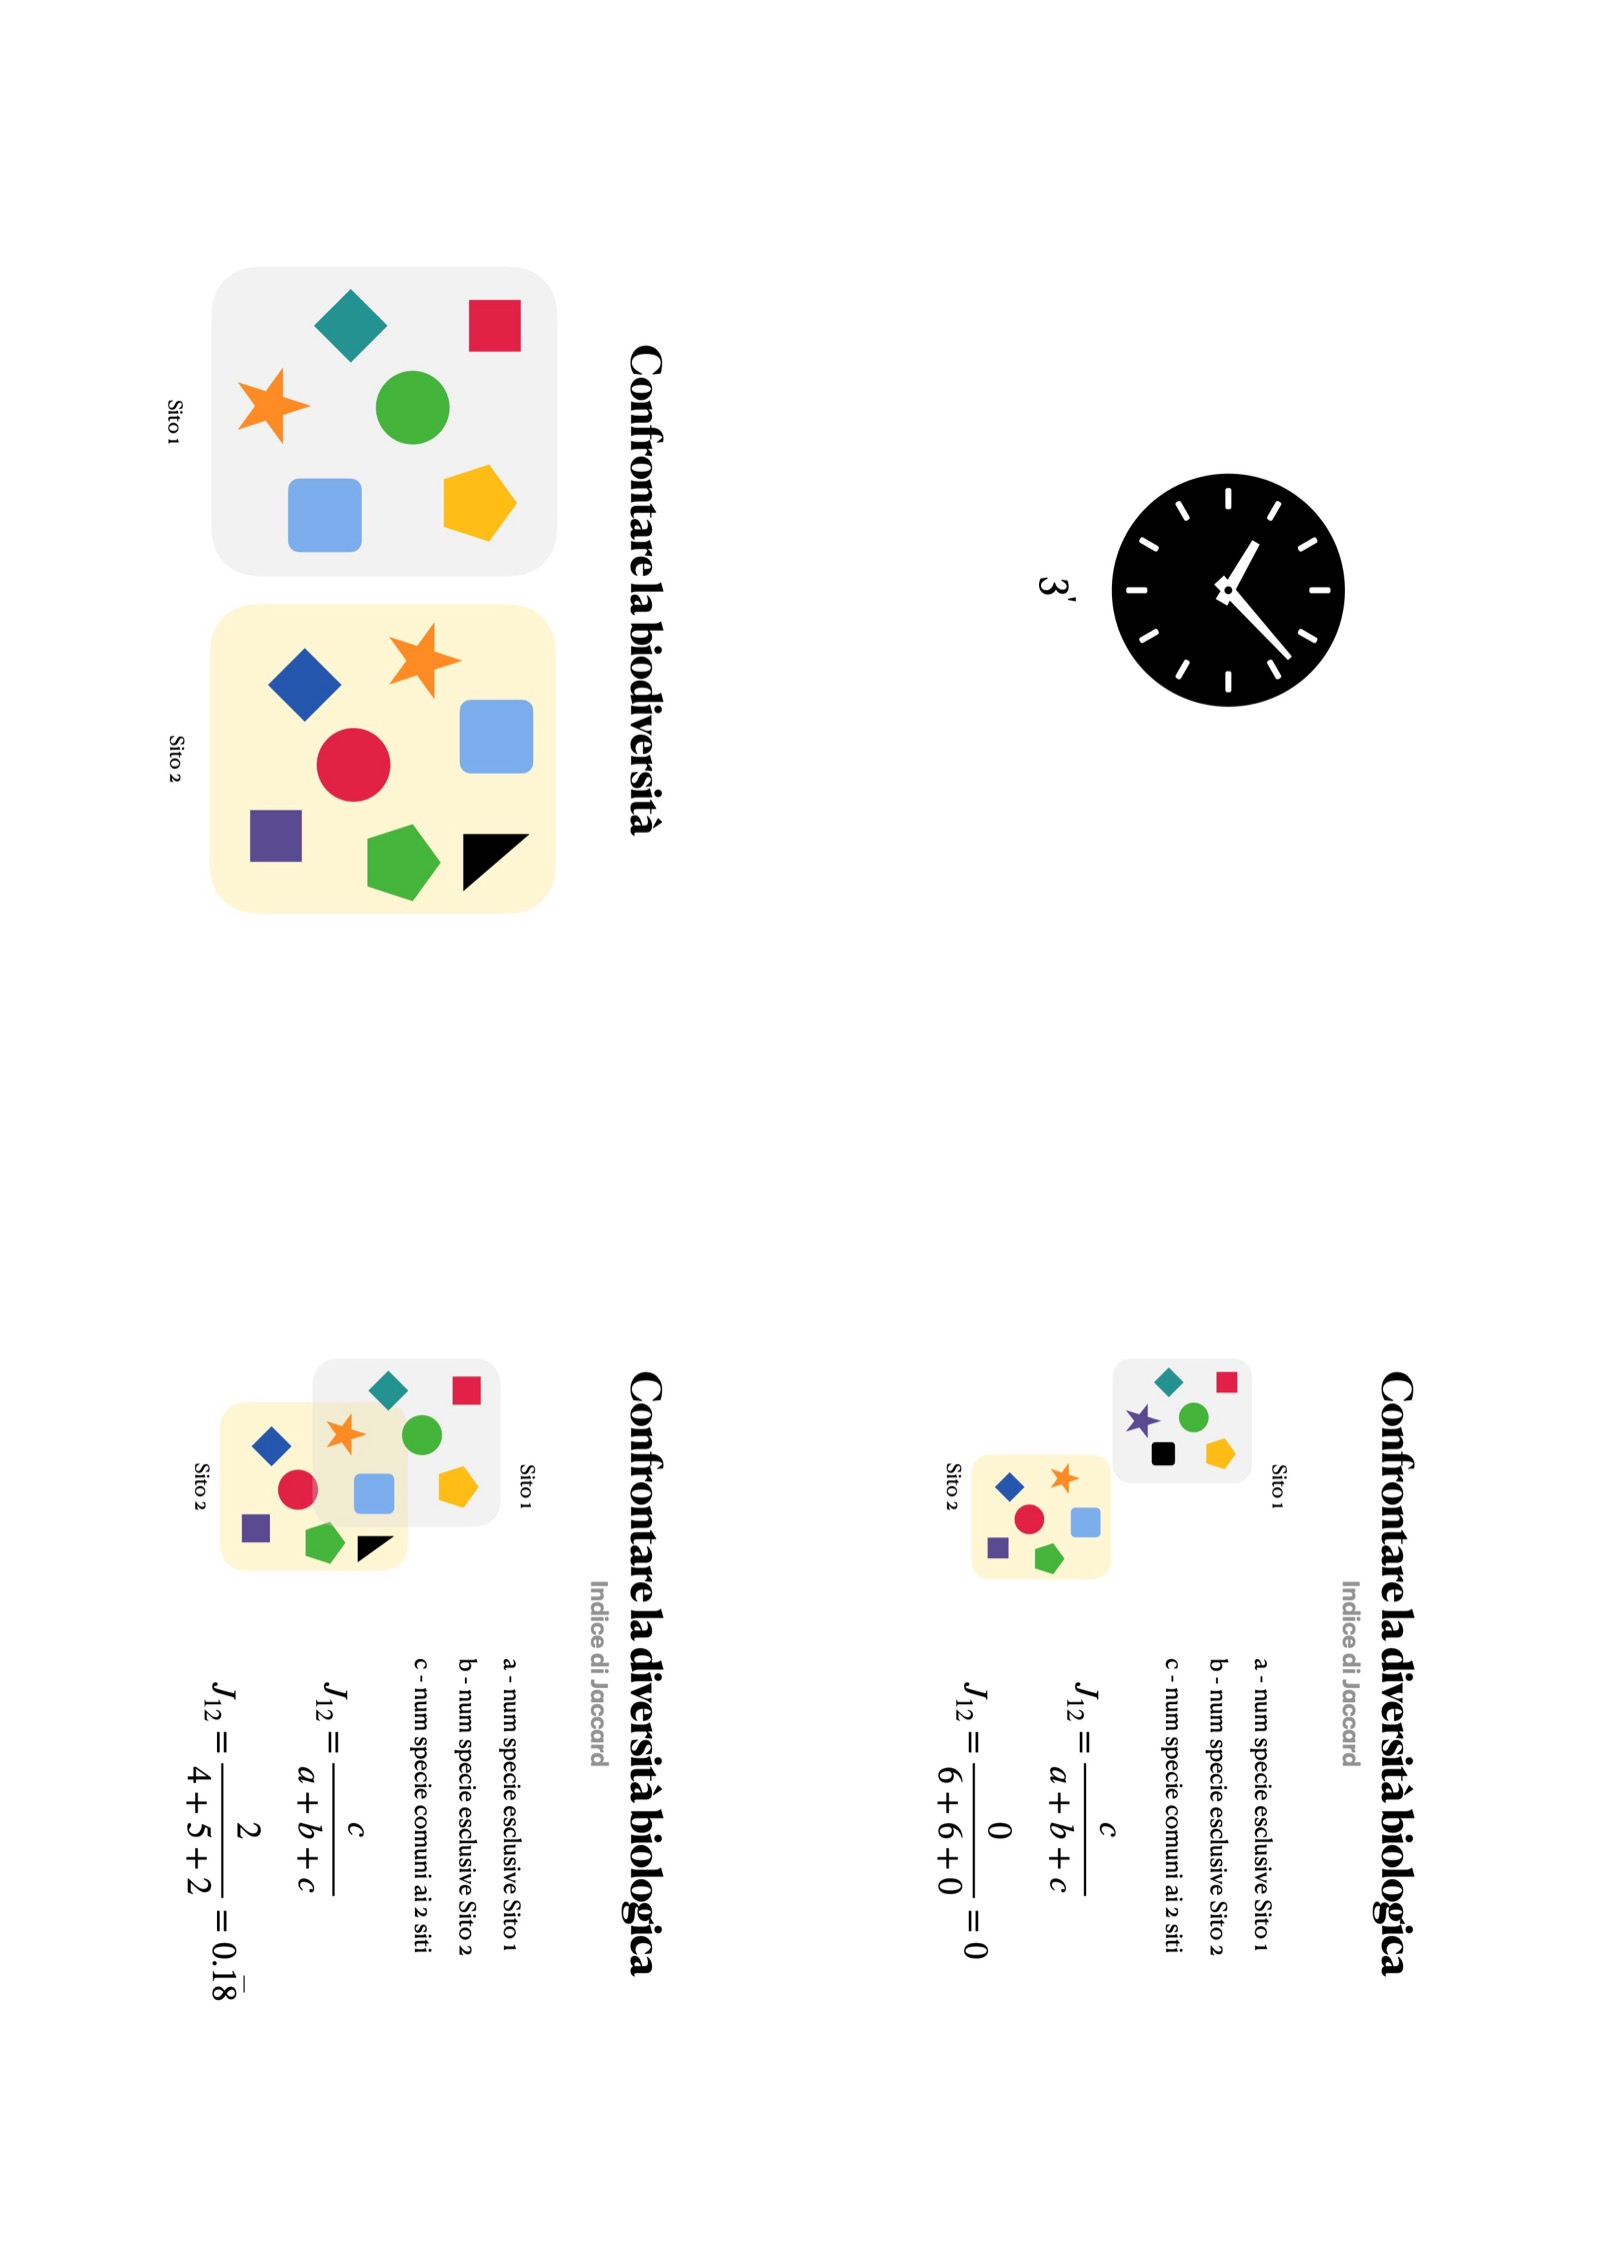
\includegraphics[keepaspectratio]{./figs/pctoREC/diversityRECSpoleto01 4-4.jpeg}}

\pandocbounded{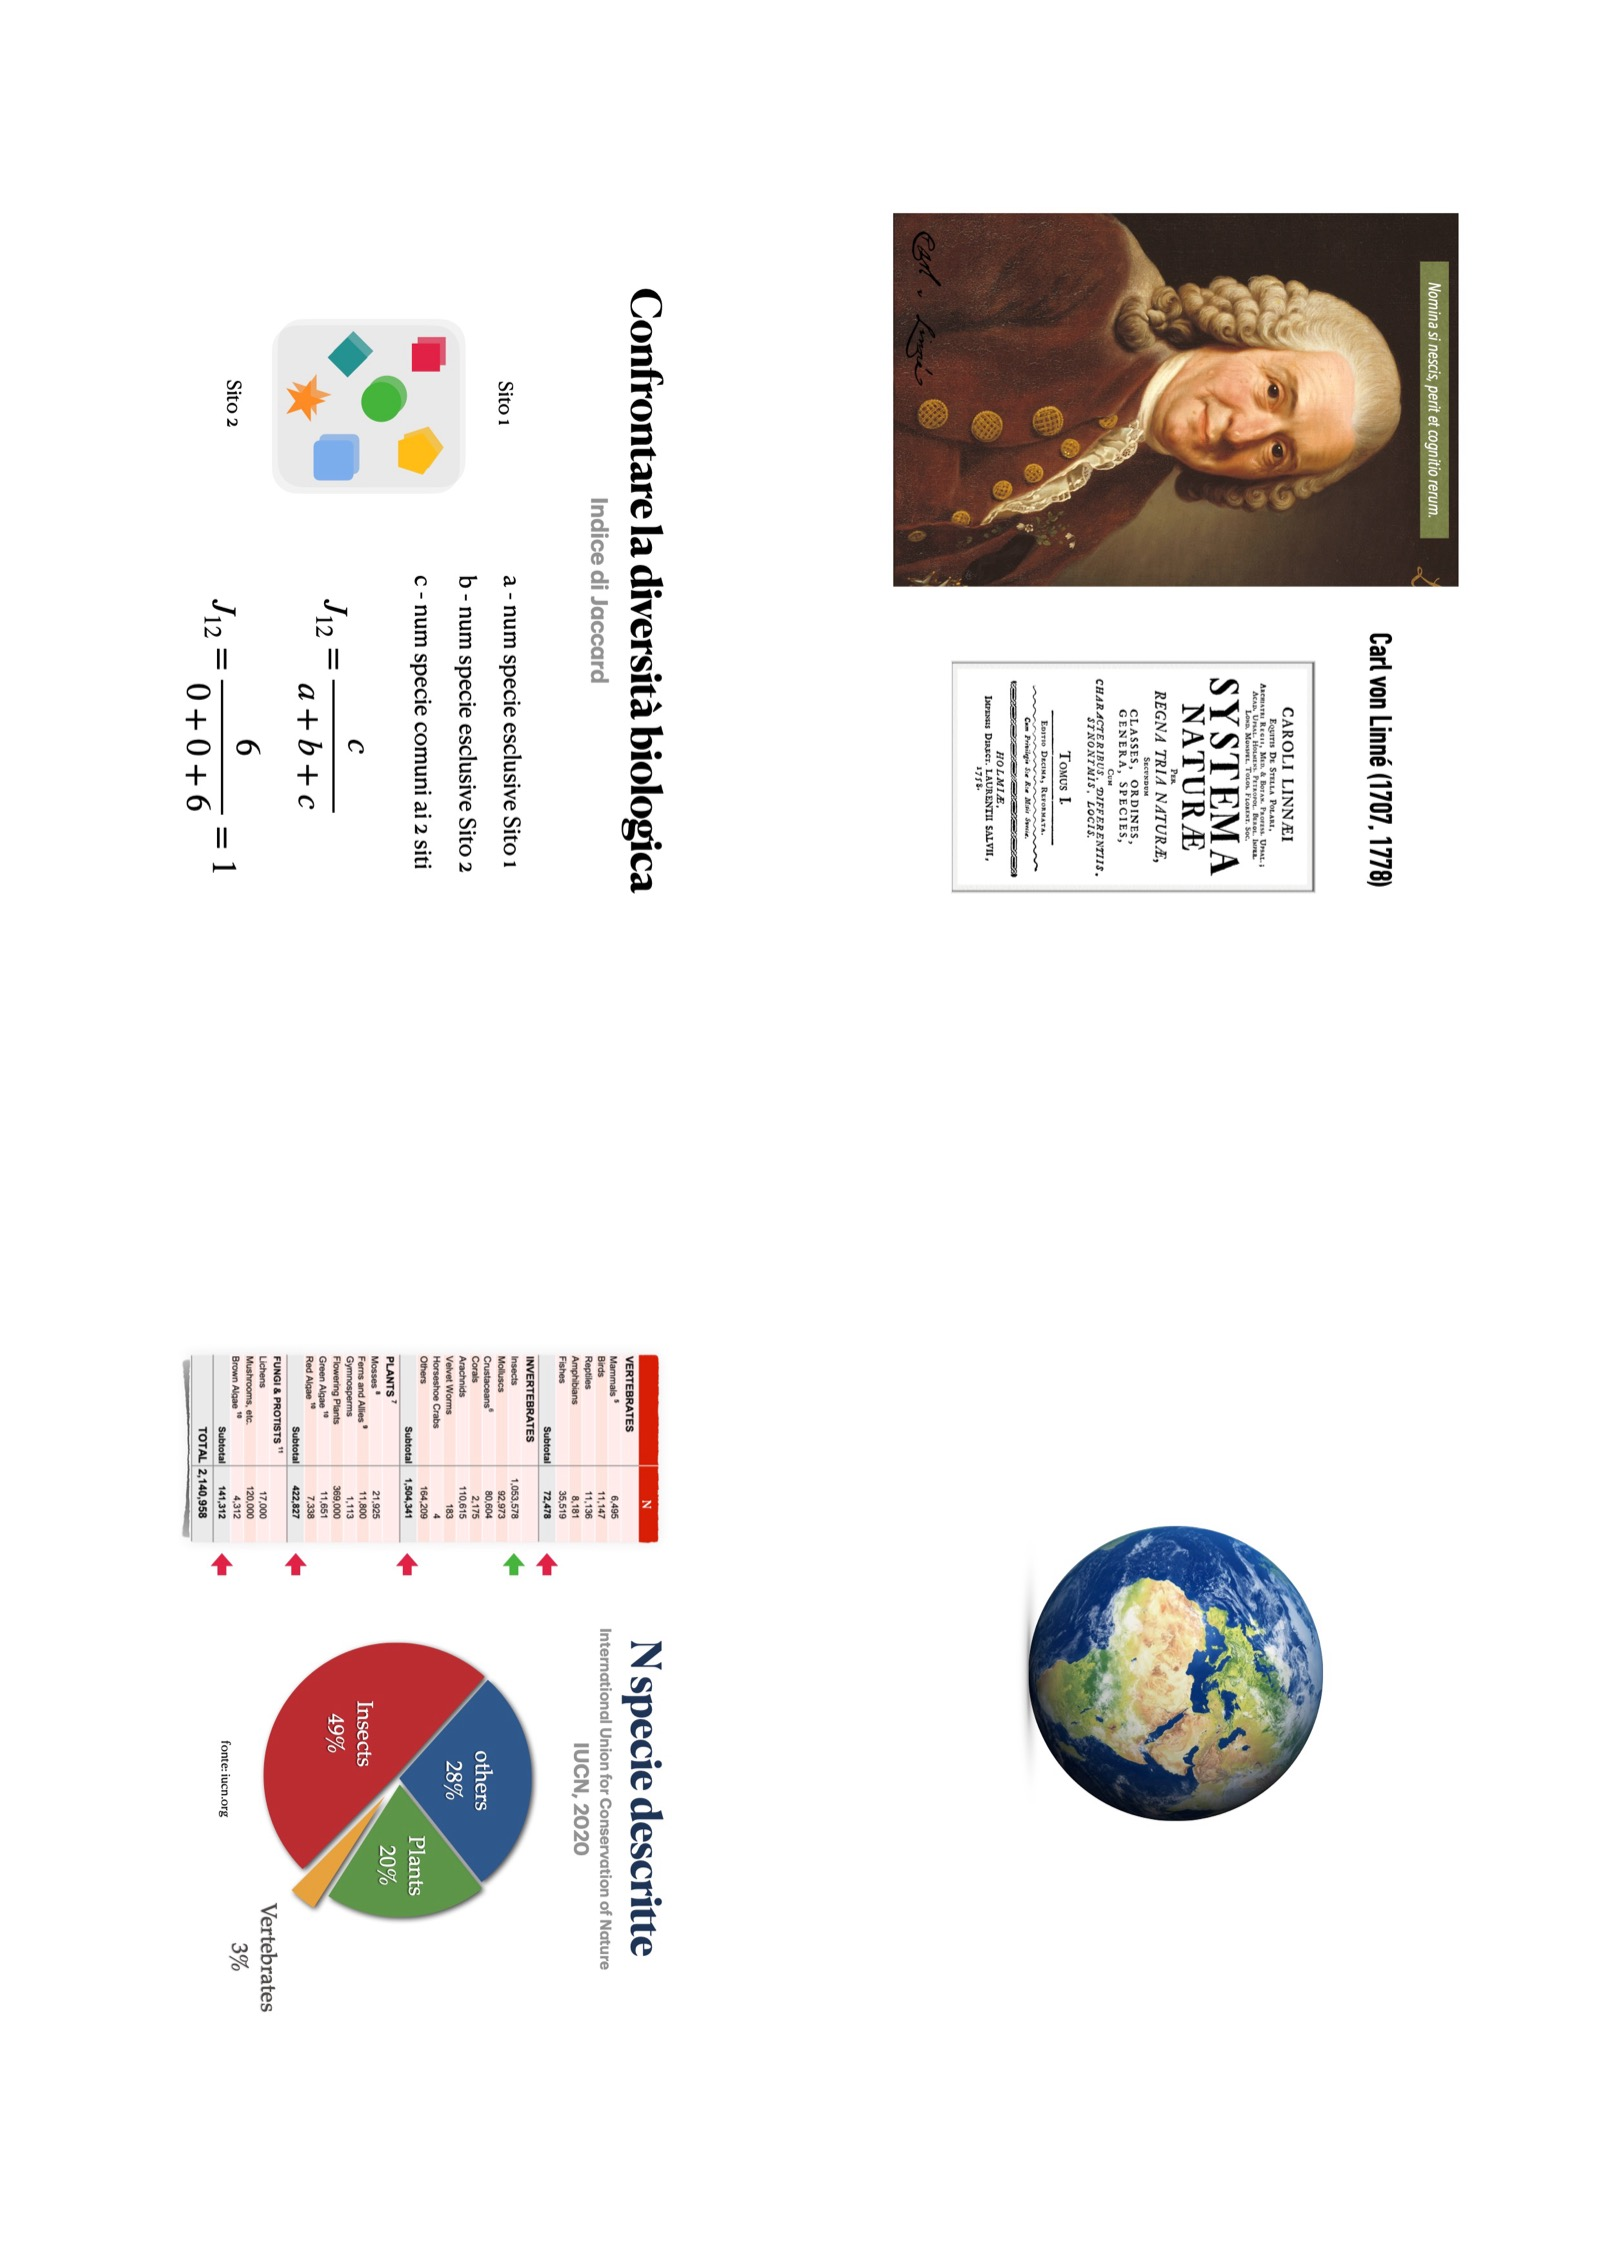
\includegraphics[keepaspectratio]{./figs/pctoREC/diversityRECSpoleto01 5-5.jpeg}}

\pandocbounded{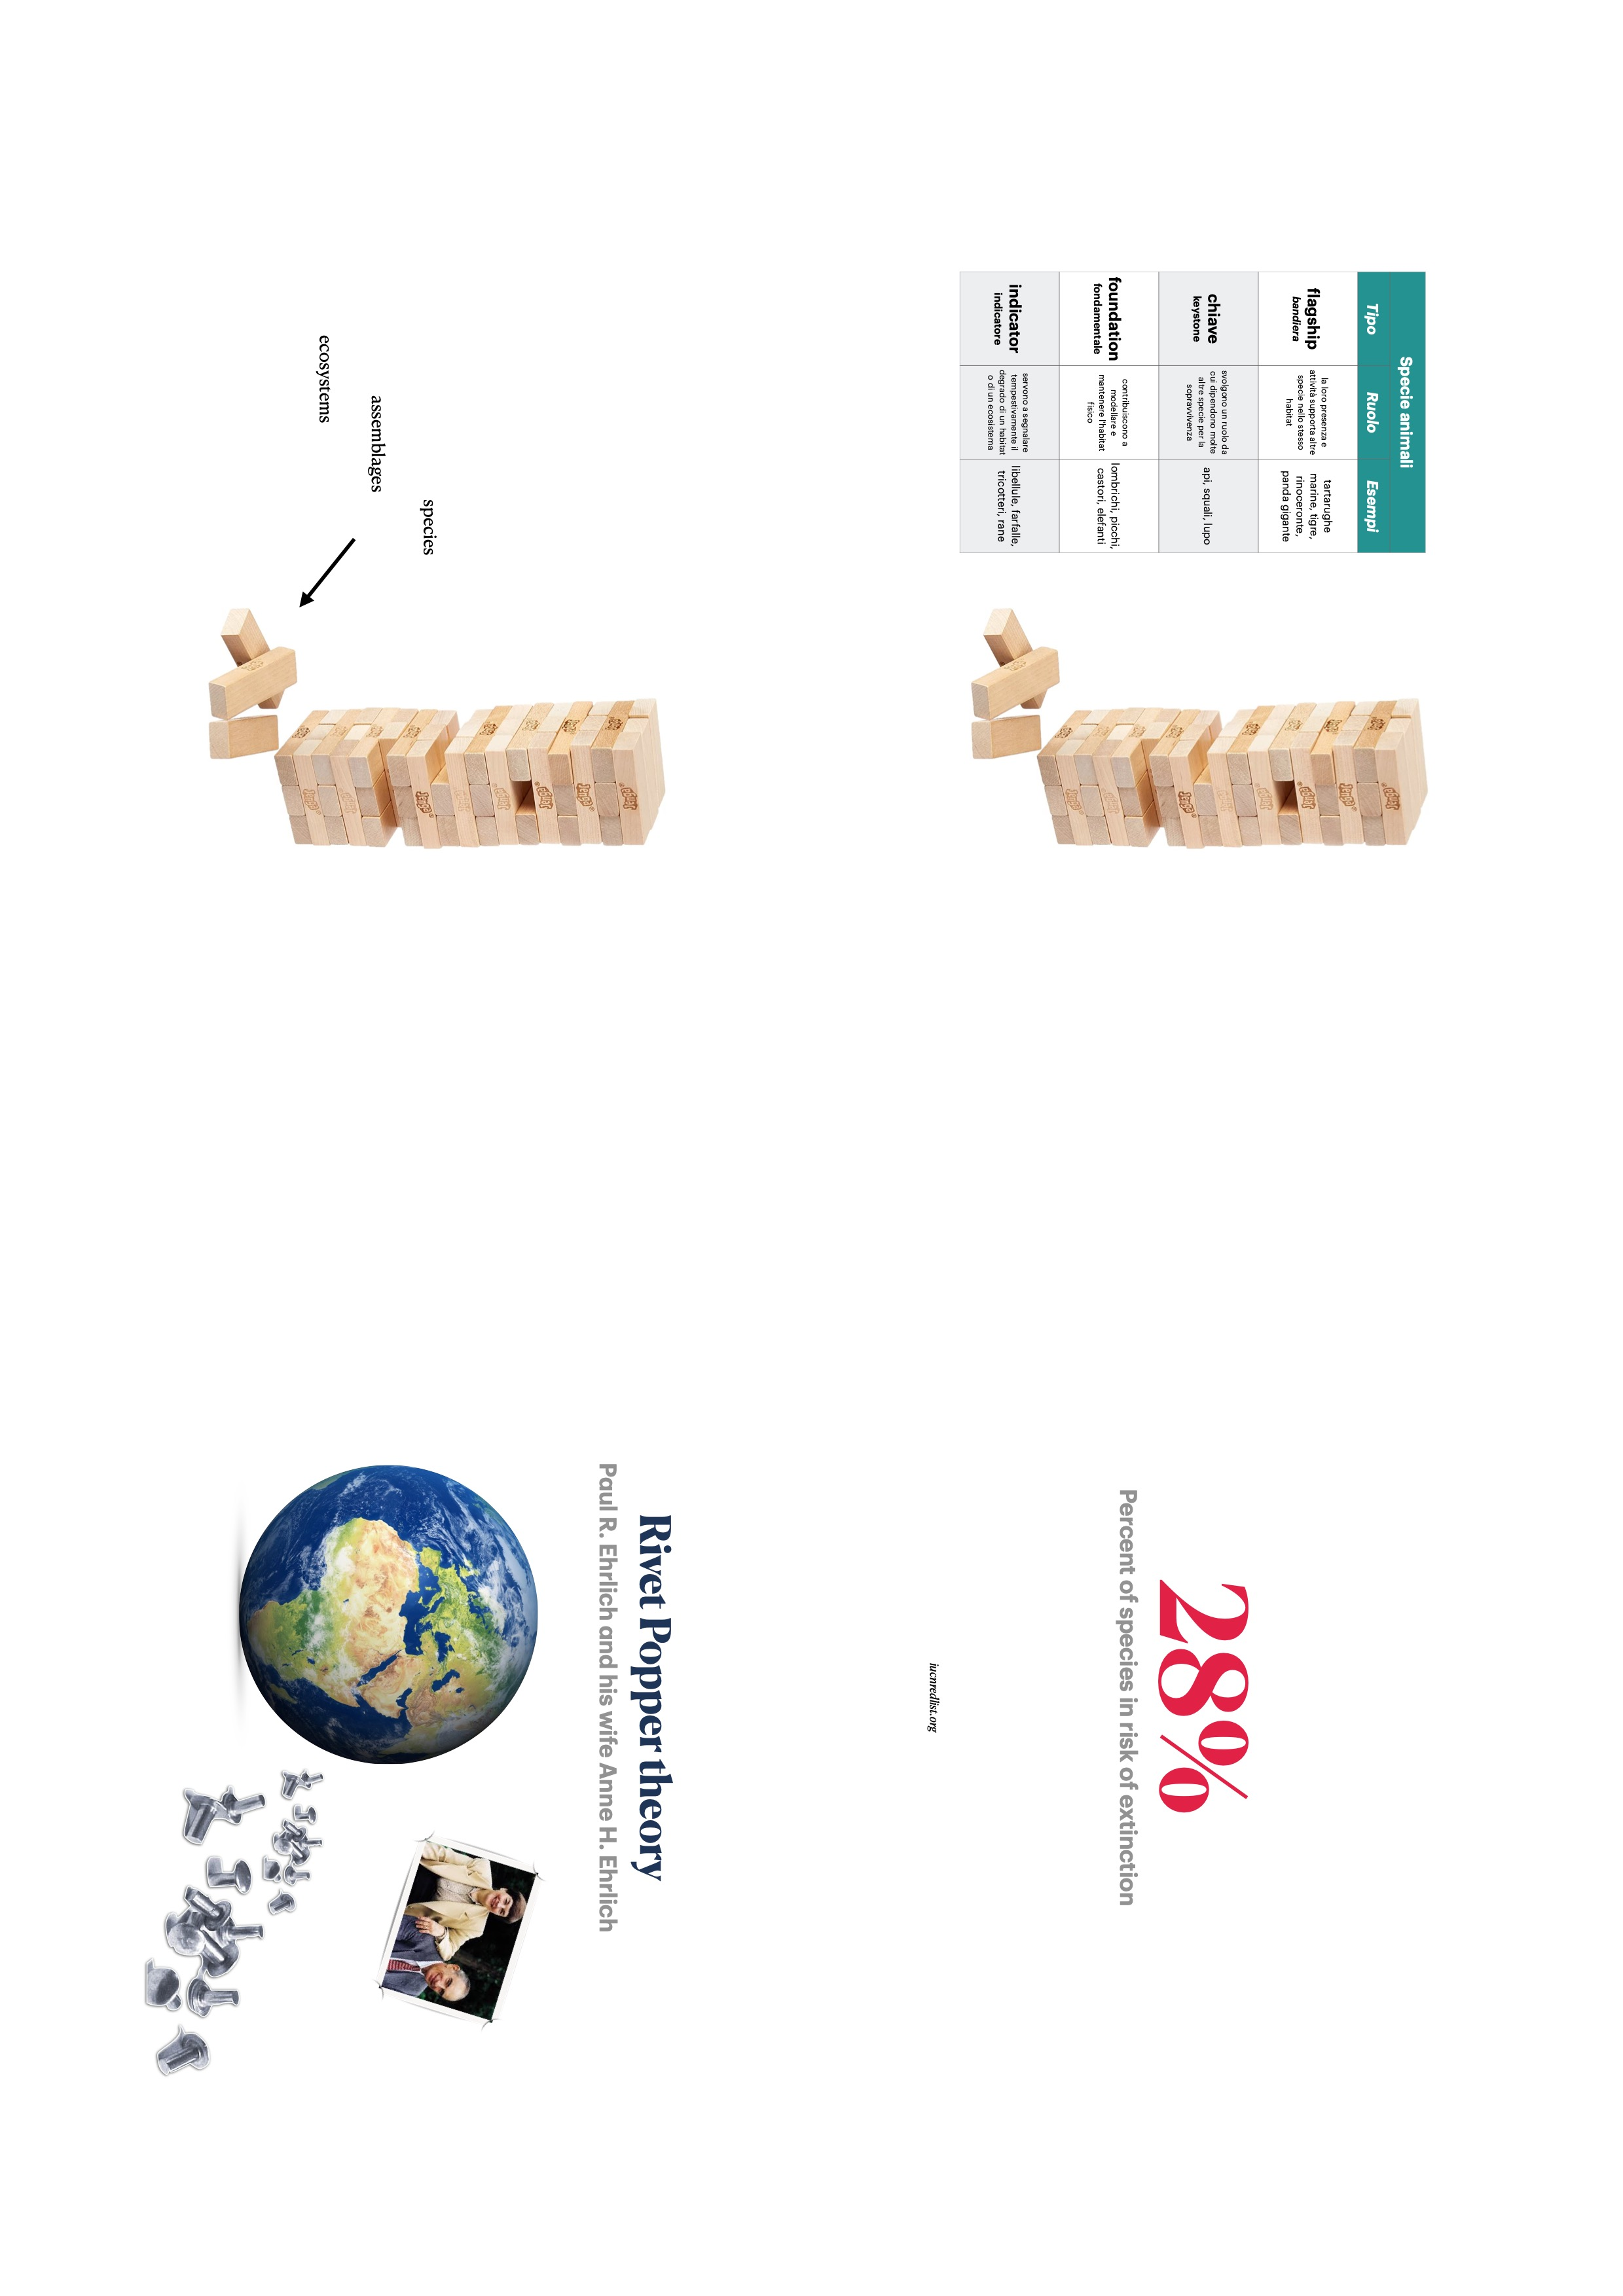
\includegraphics[keepaspectratio]{./figs/pctoREC/diversityRECSpoleto01 6-6.jpeg}}

\pandocbounded{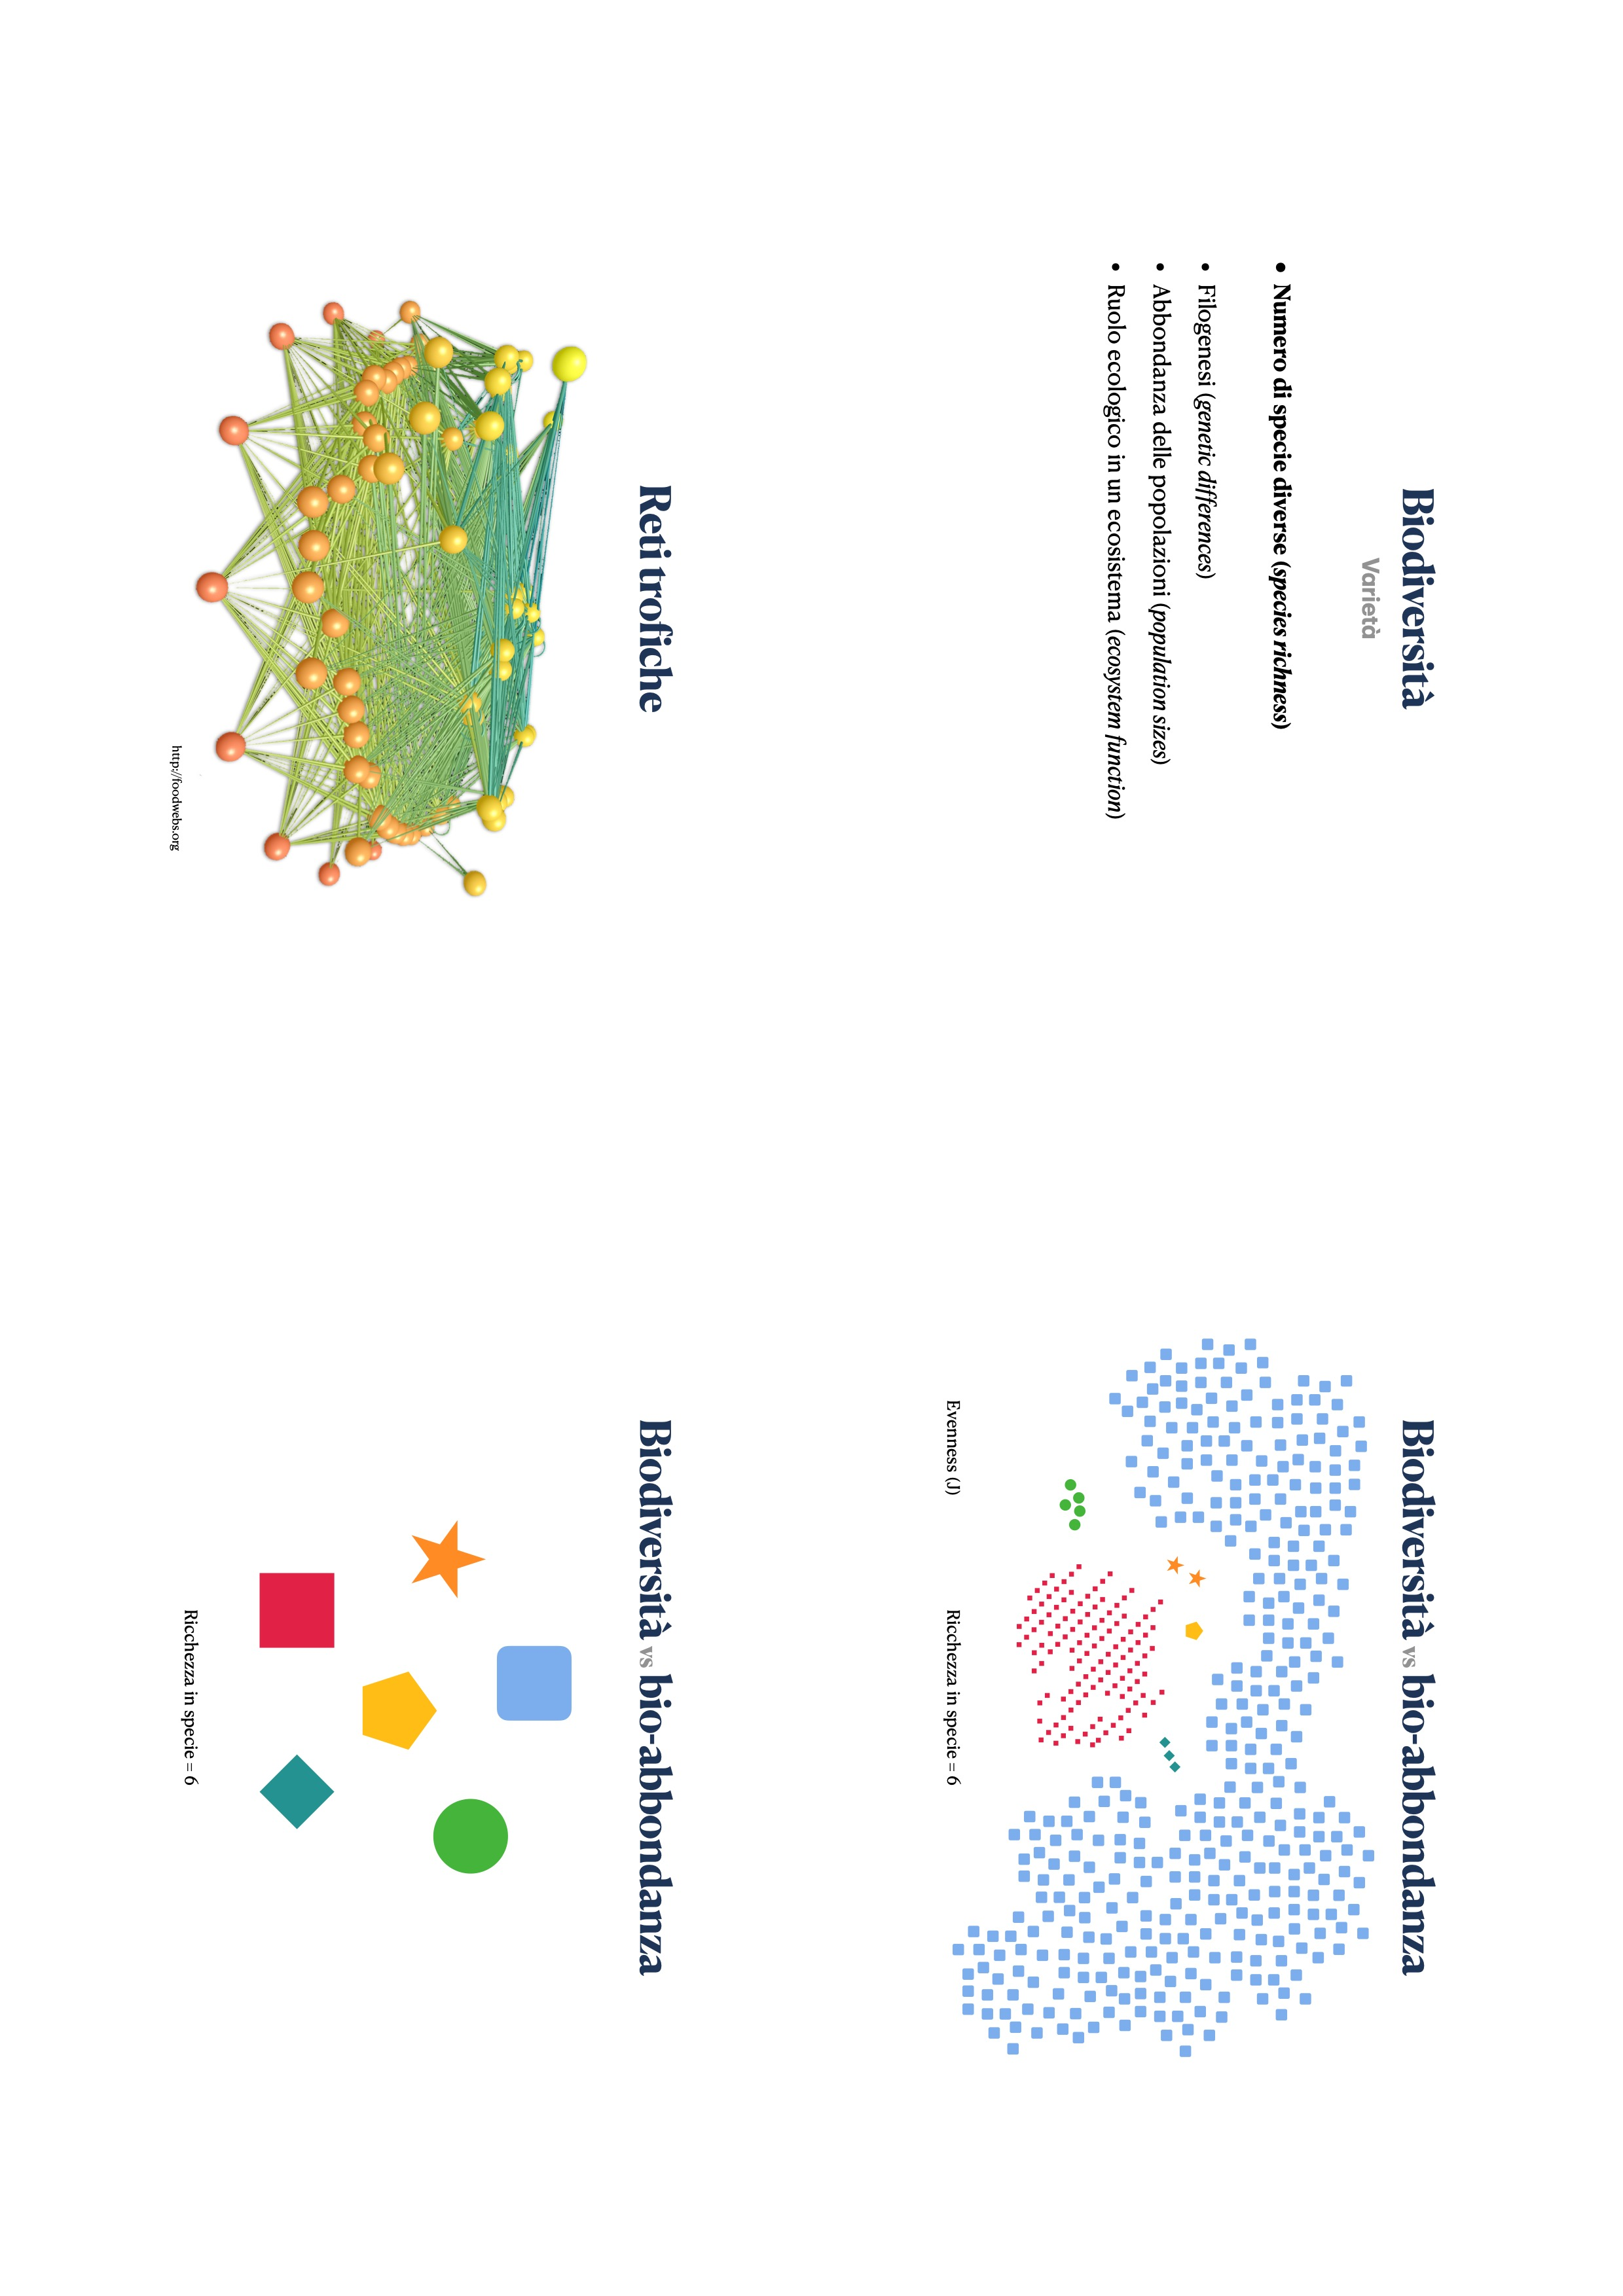
\includegraphics[keepaspectratio]{./figs/pctoREC/diversityRECSpoleto01 7-7.jpeg}}

\pandocbounded{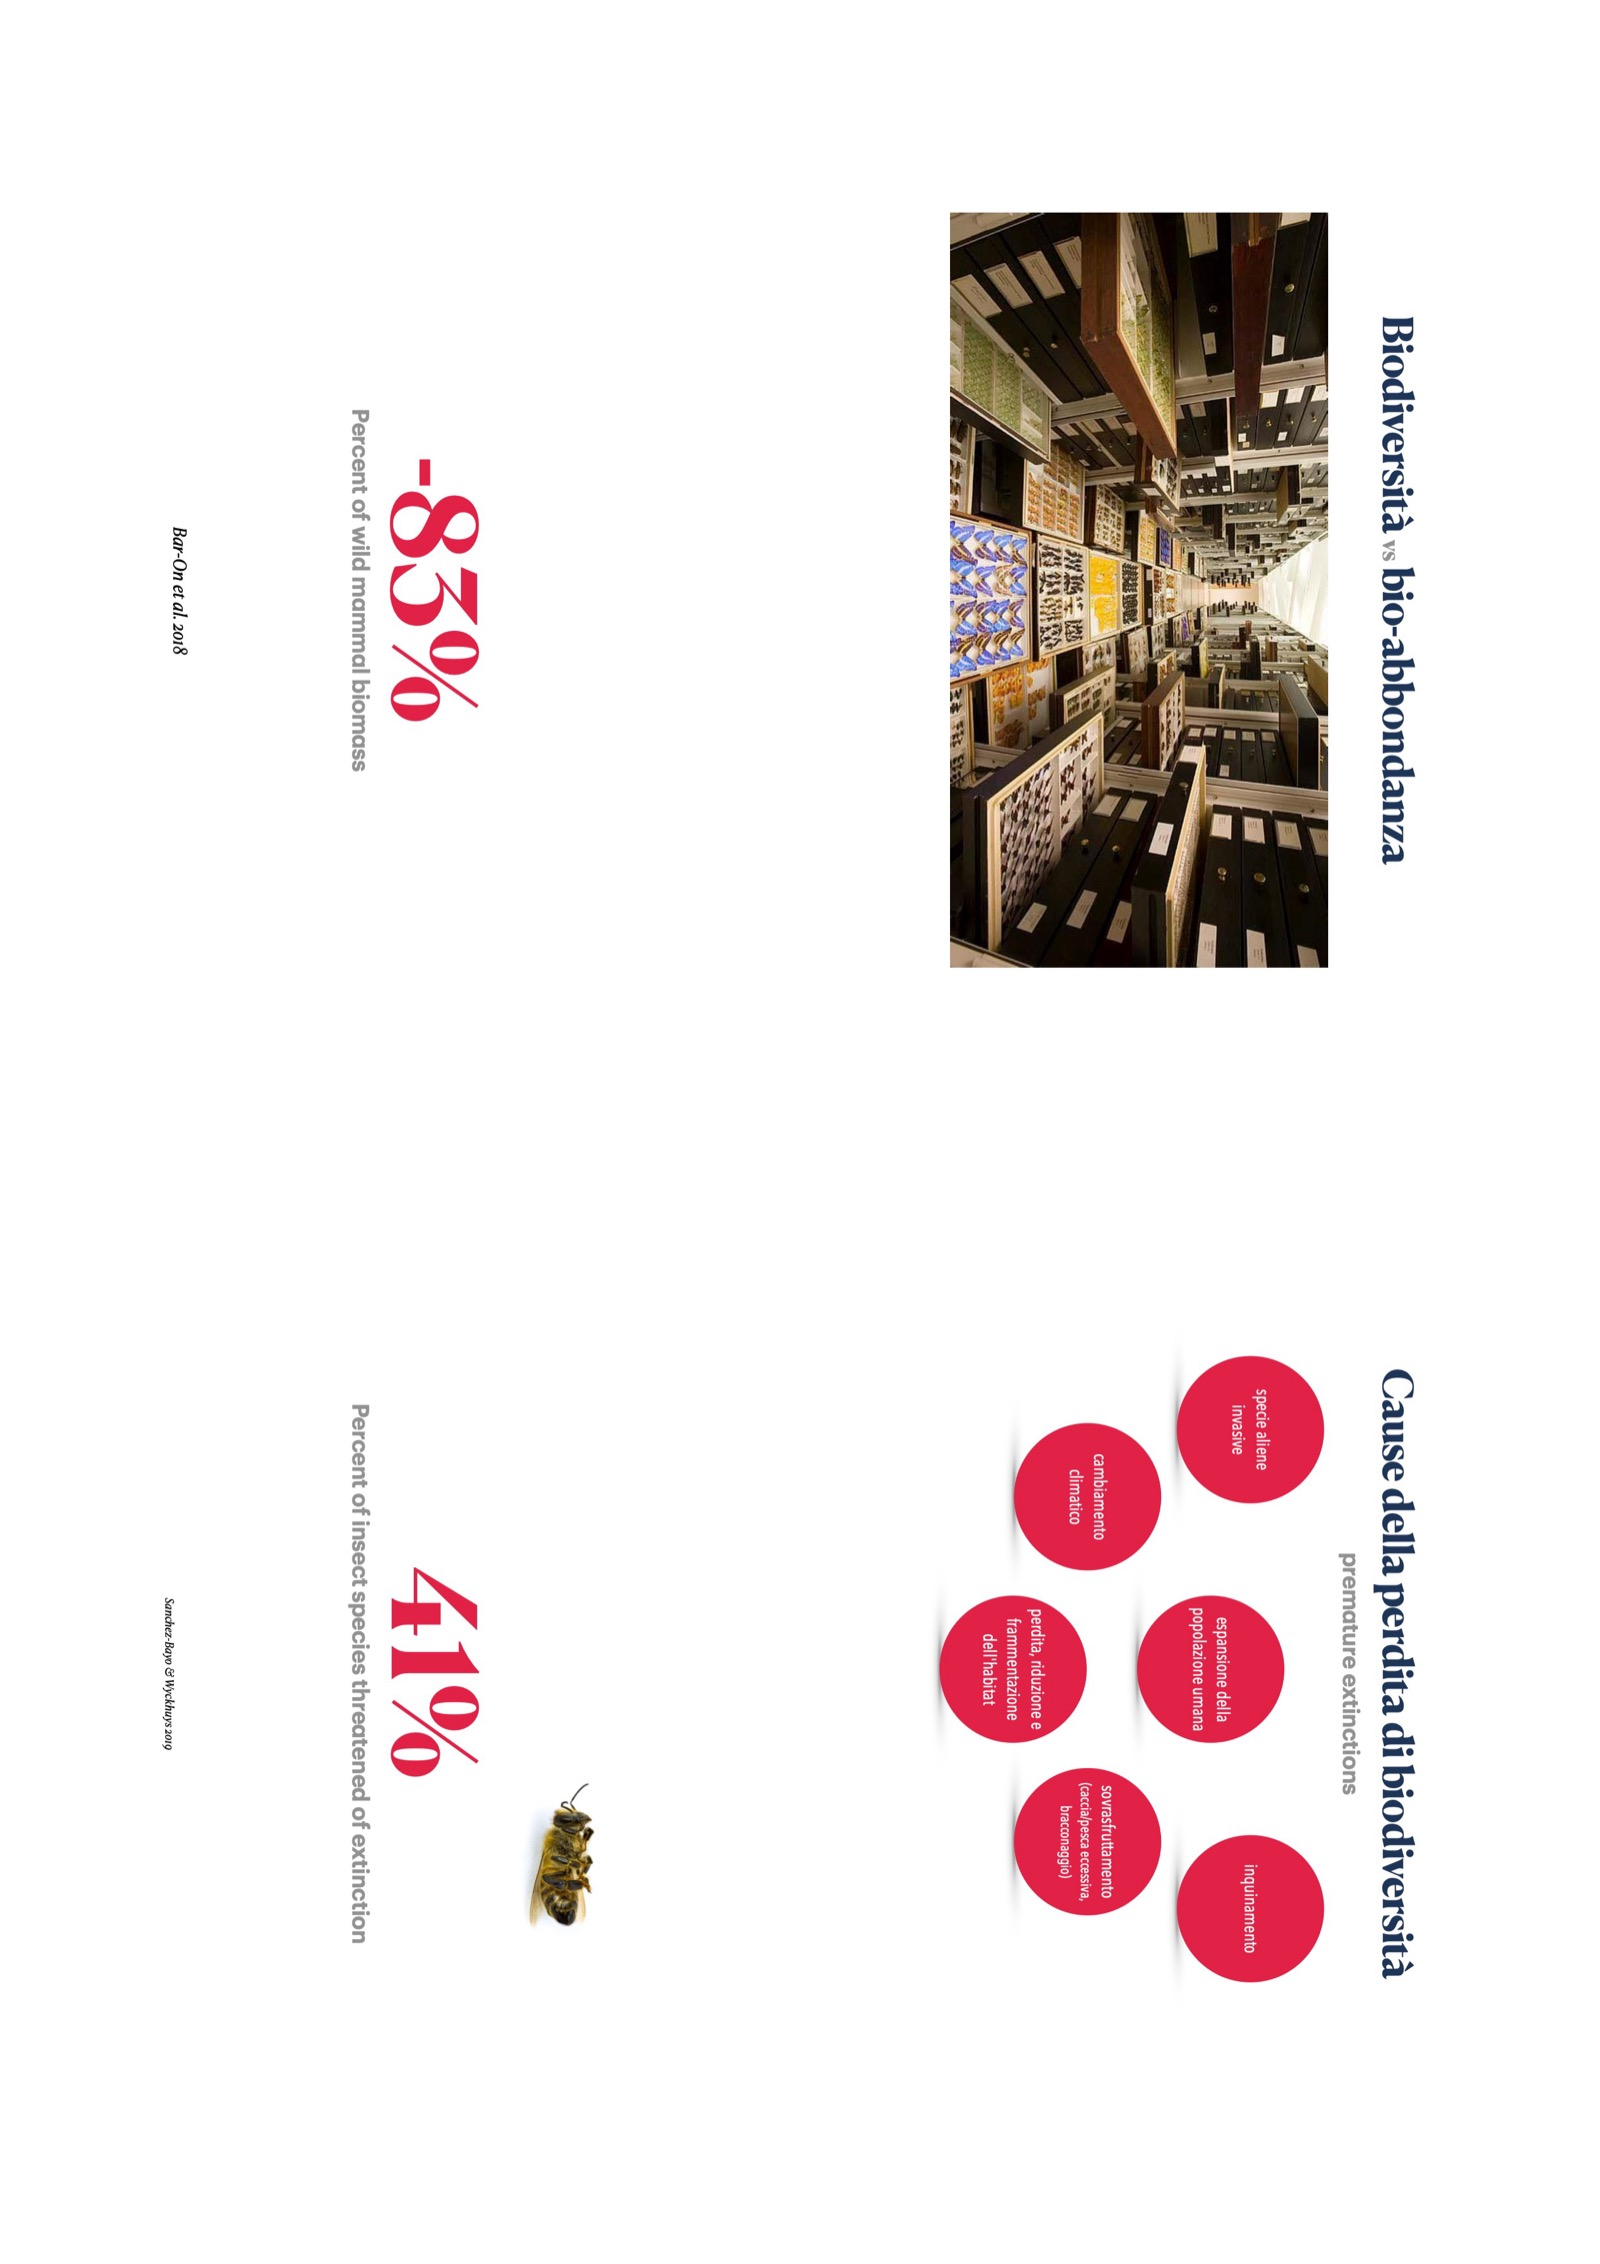
\includegraphics[keepaspectratio]{./figs/pctoREC/diversityRECSpoleto01 8-8.jpeg}}

\pandocbounded{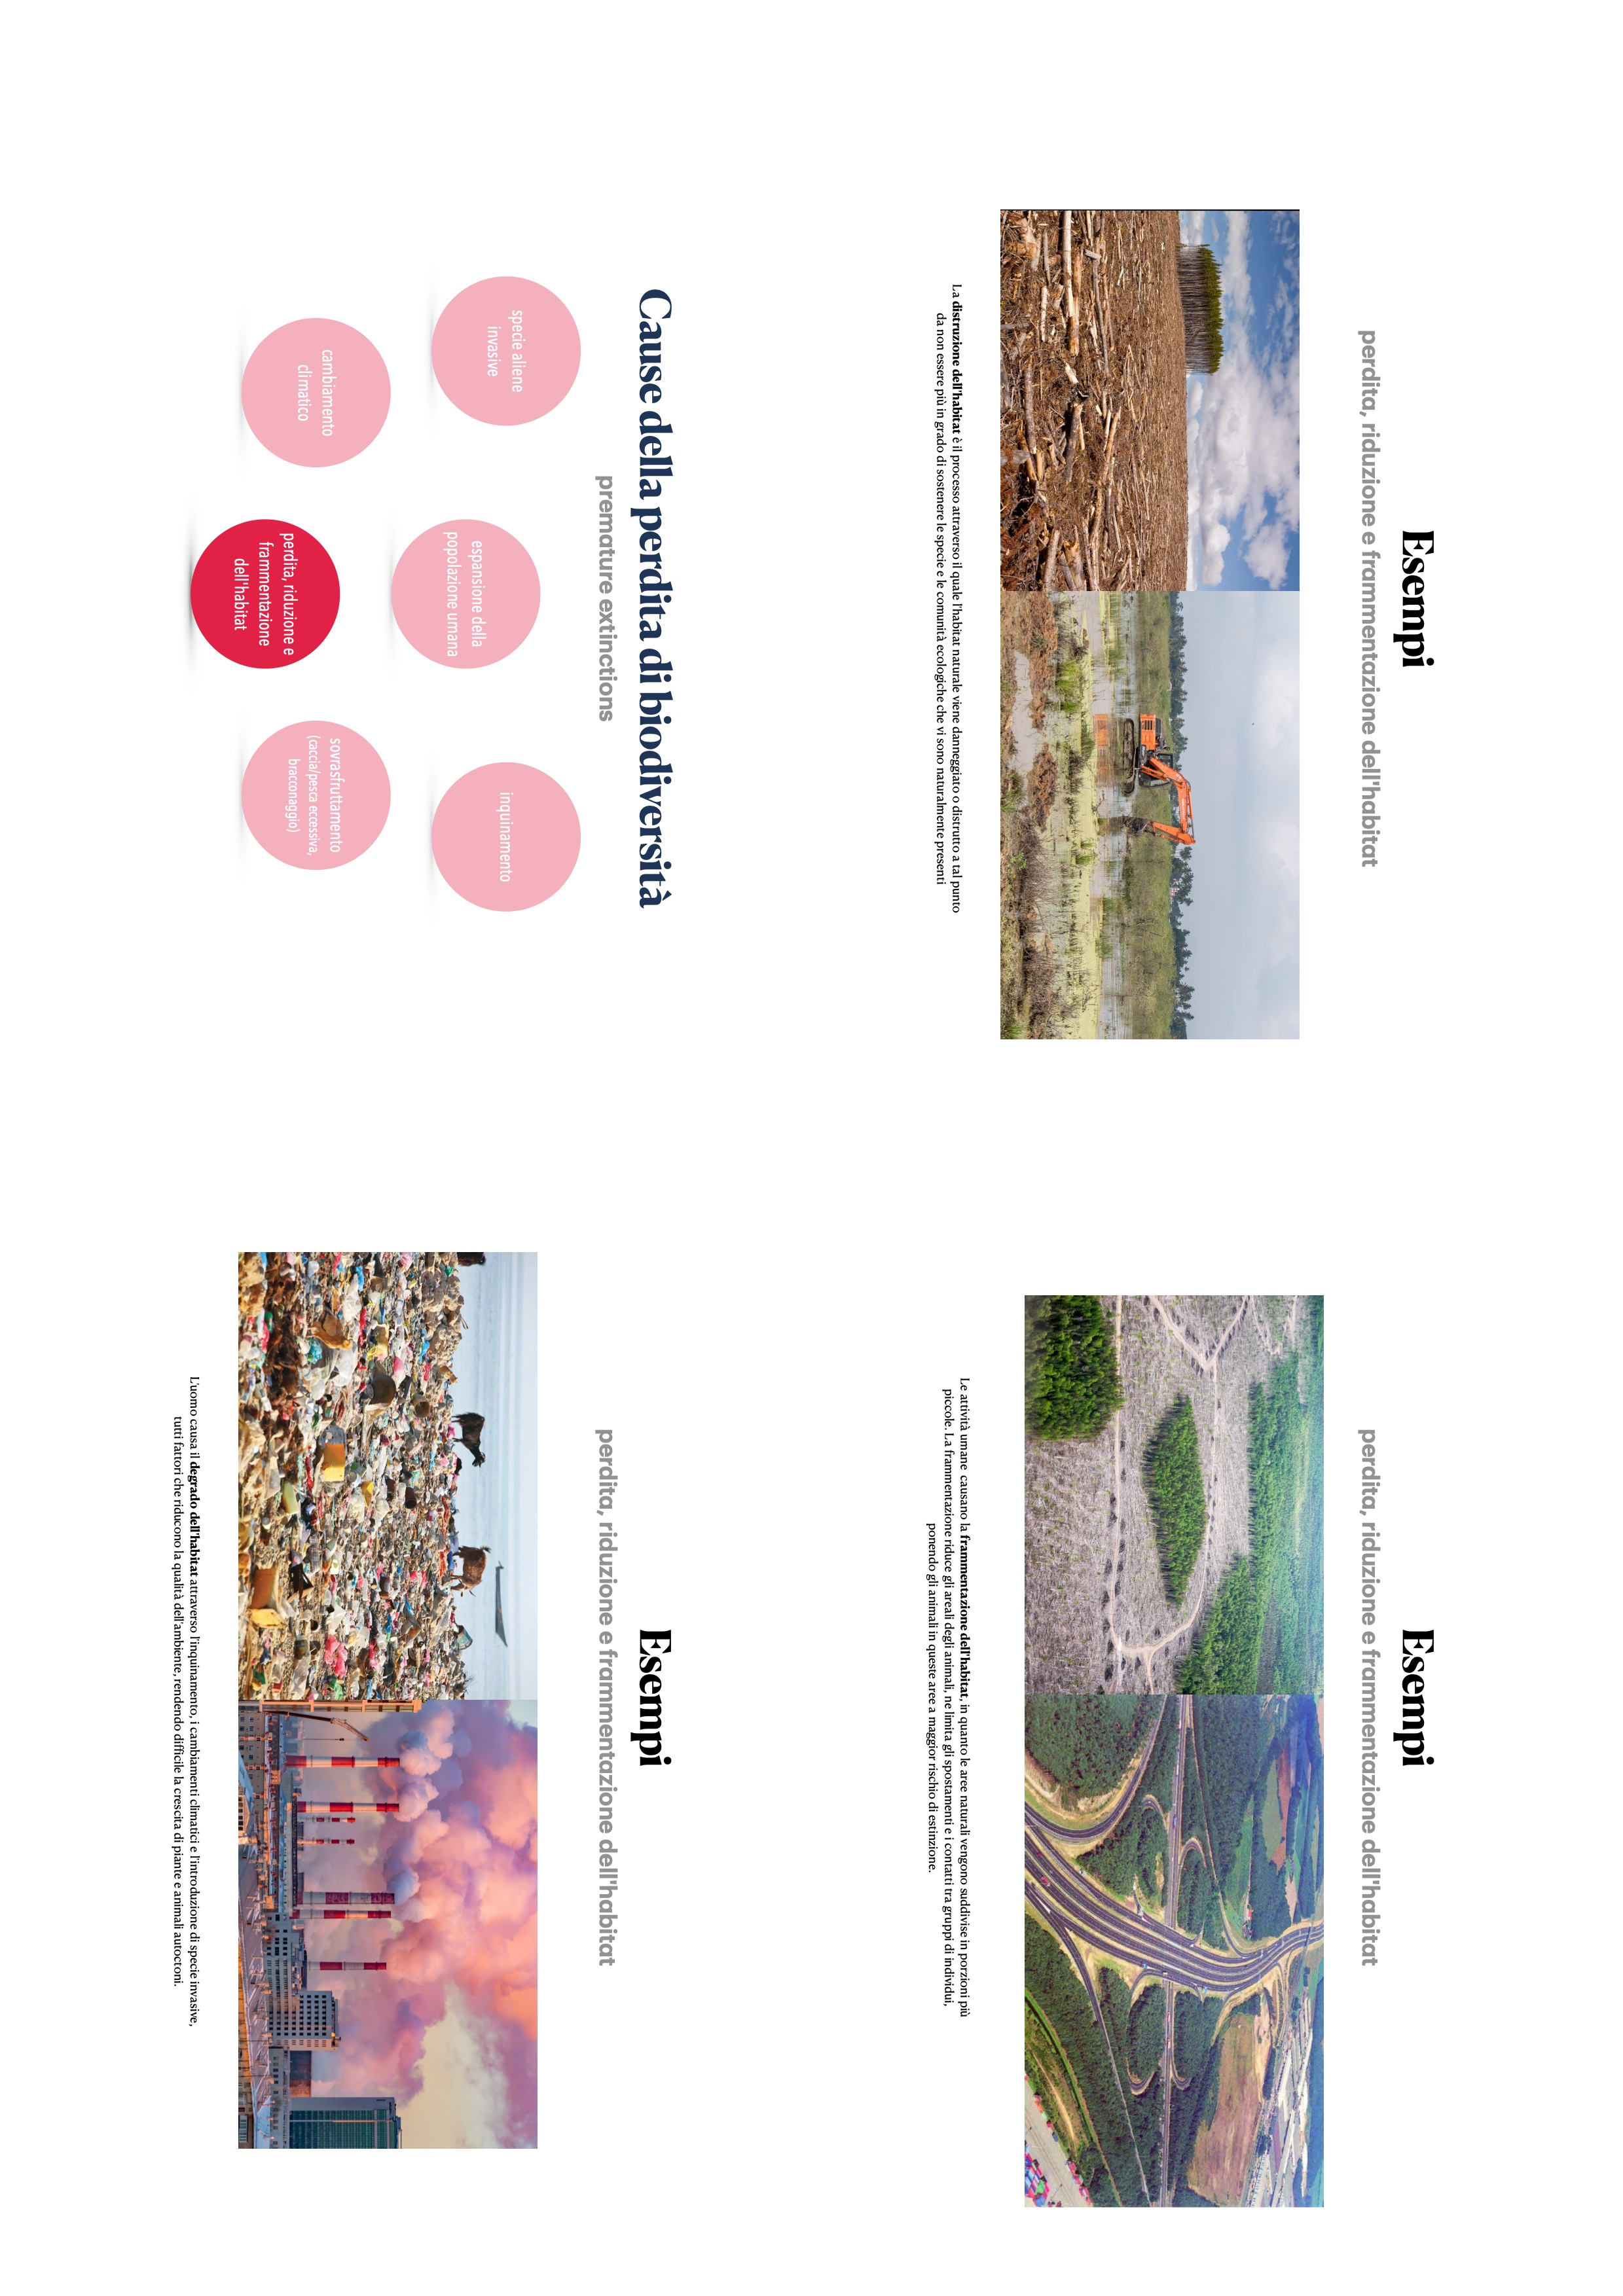
\includegraphics[keepaspectratio]{./figs/pctoREC/diversityRECSpoleto01 9-9.jpeg}}

\pandocbounded{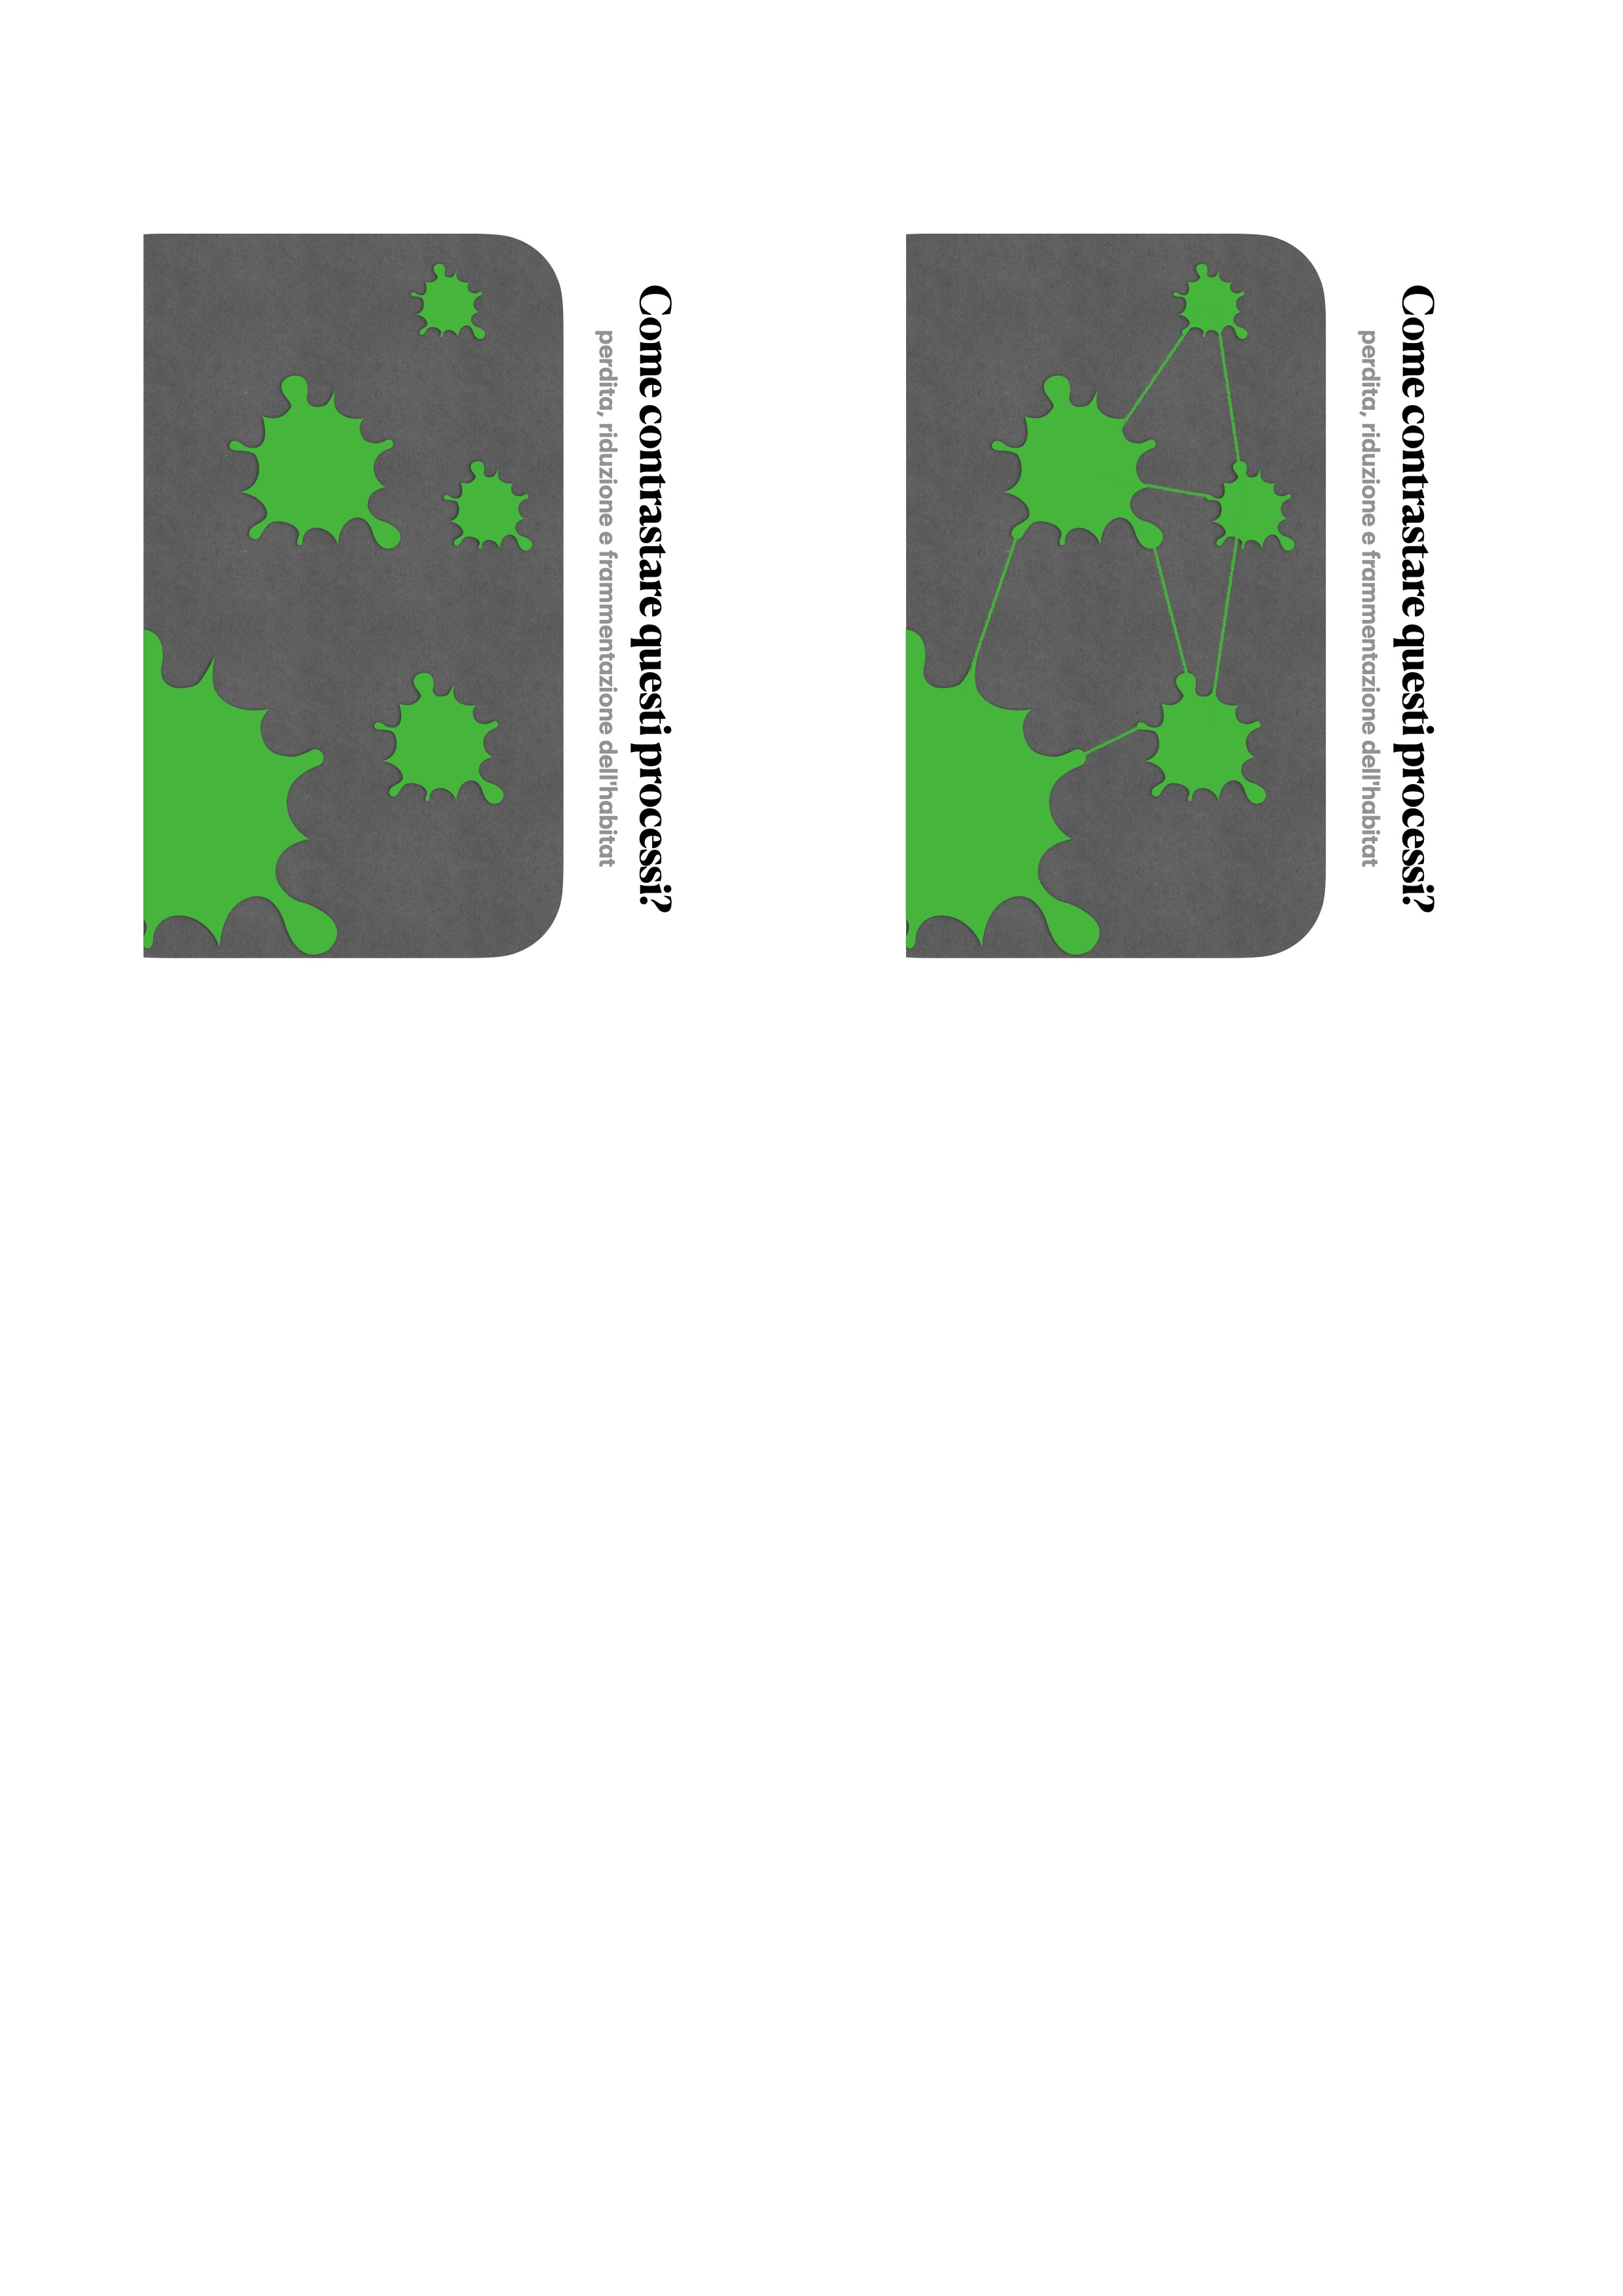
\includegraphics[keepaspectratio]{./figs/pctoREC/diversityRECSpoleto01 10-10.jpeg}}

\pandocbounded{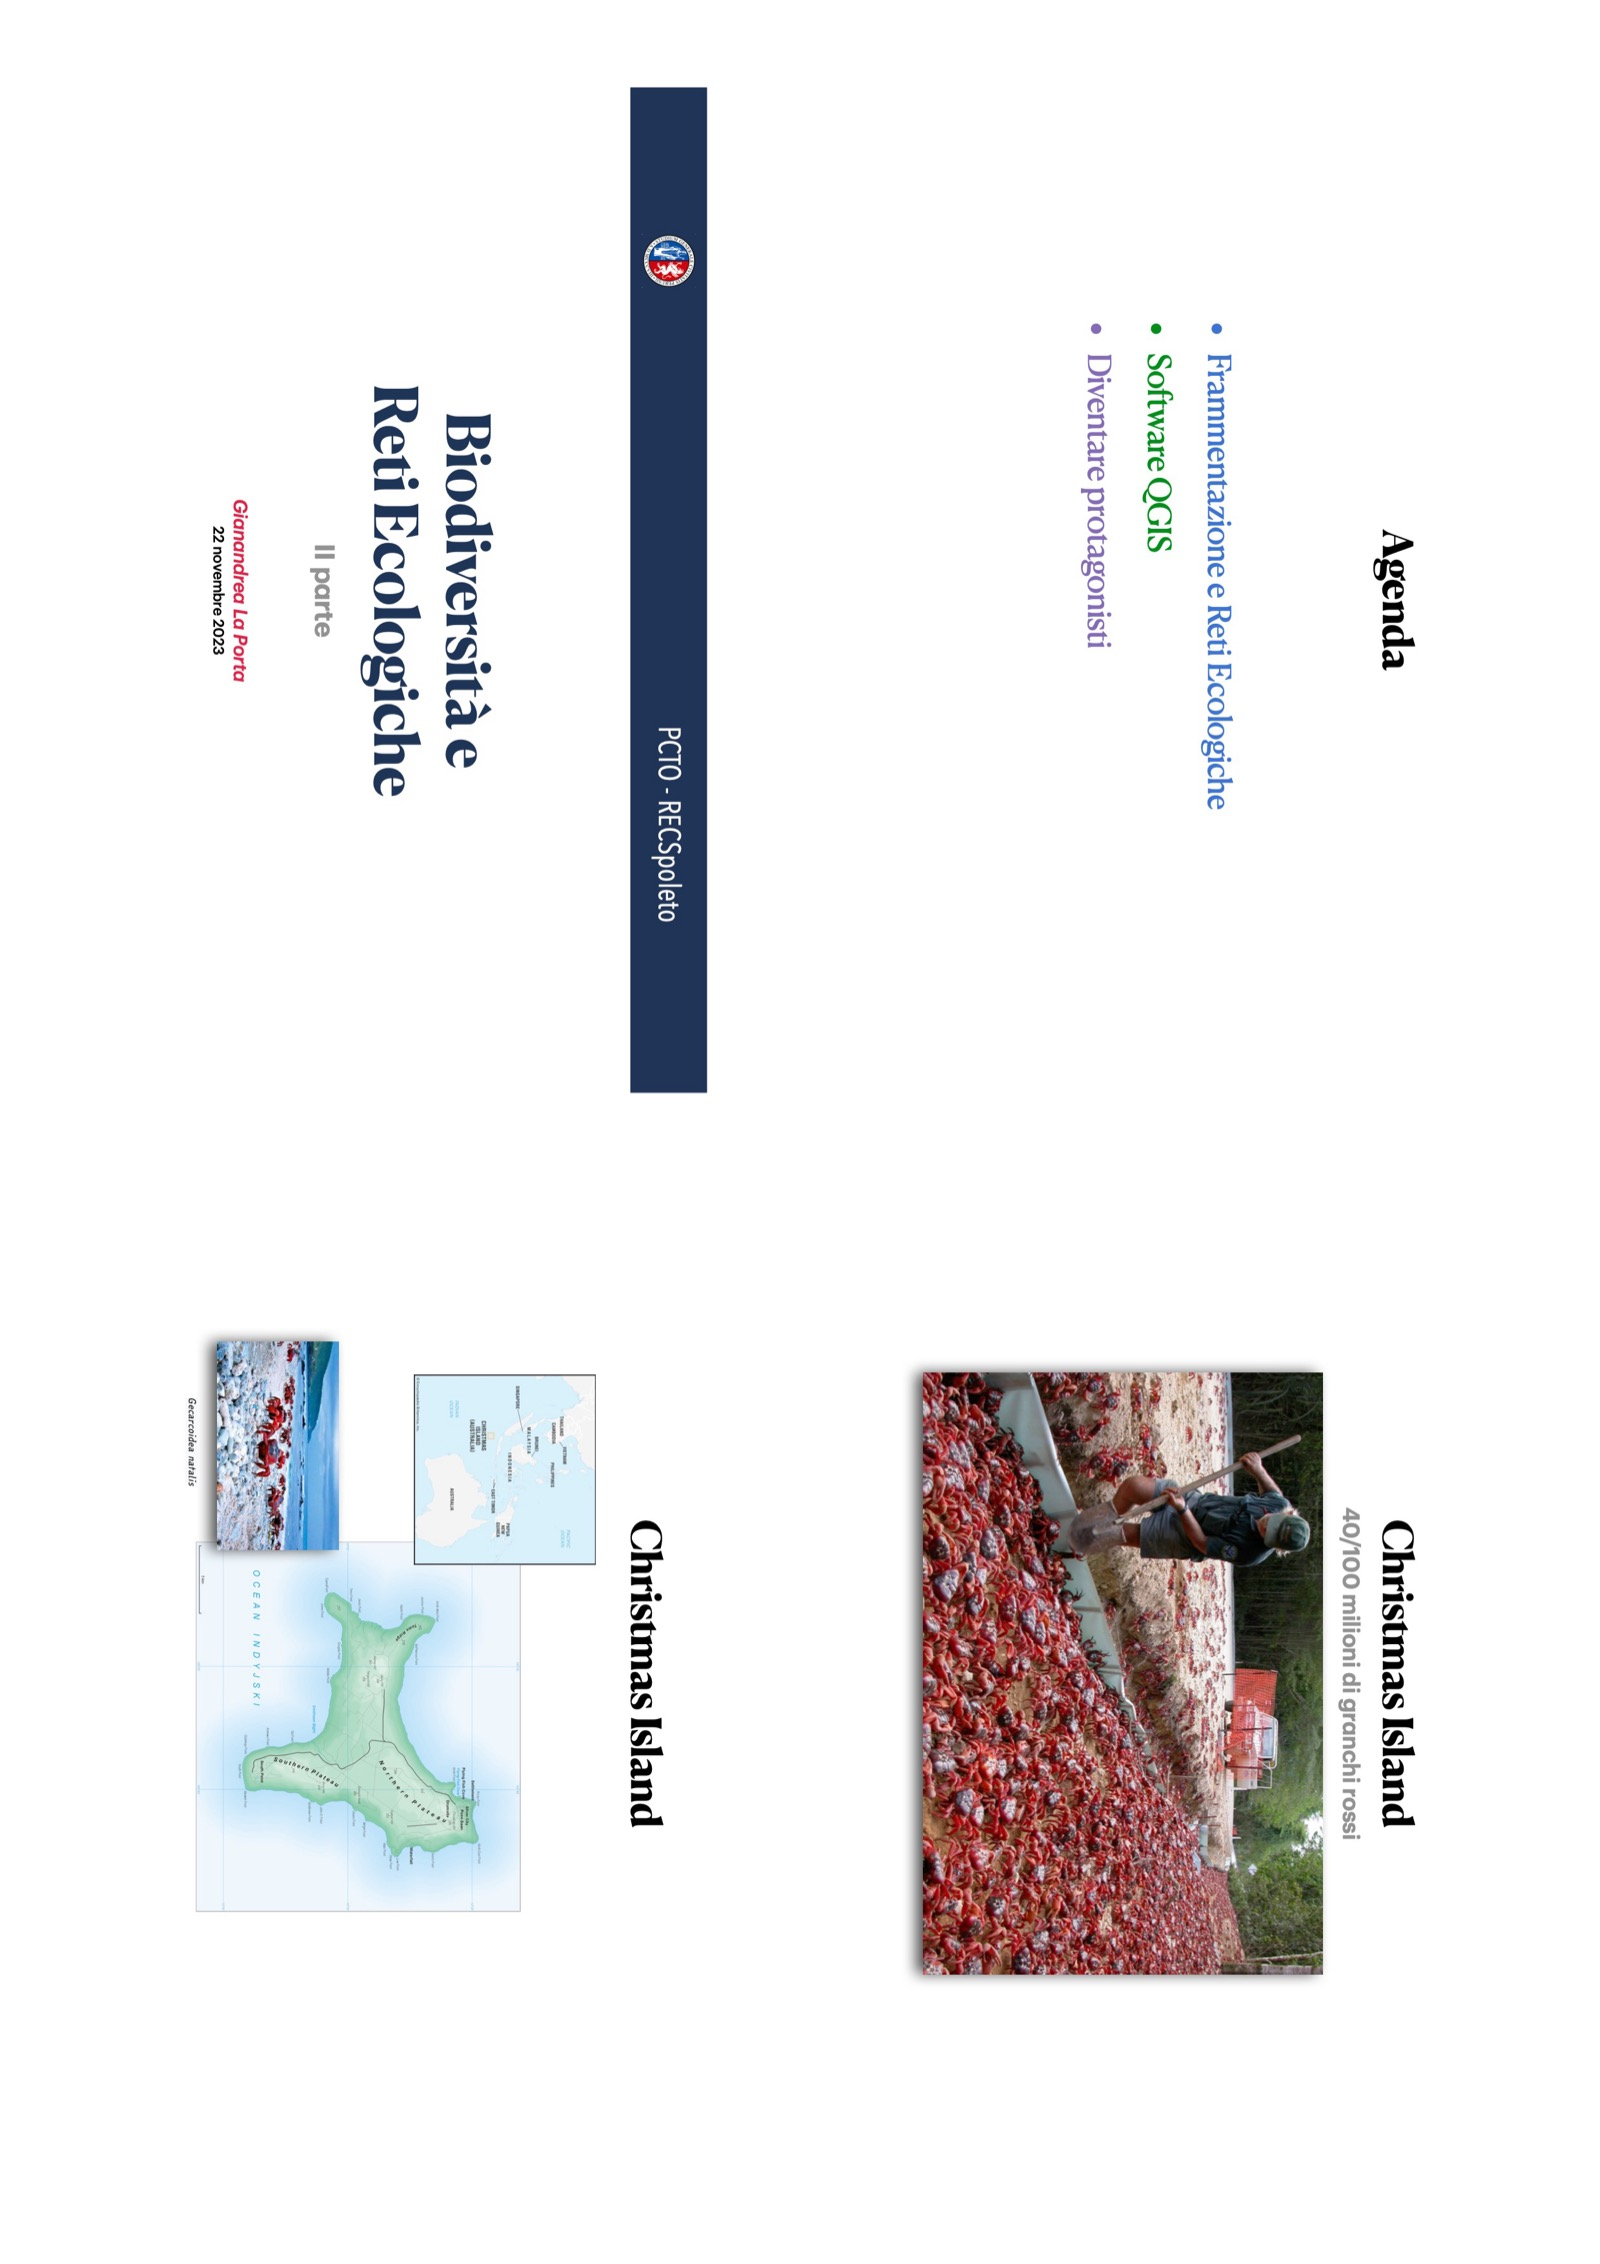
\includegraphics[keepaspectratio]{./figs/pctoREC/diversityRECSpoleto02-1.jpeg}}

\pandocbounded{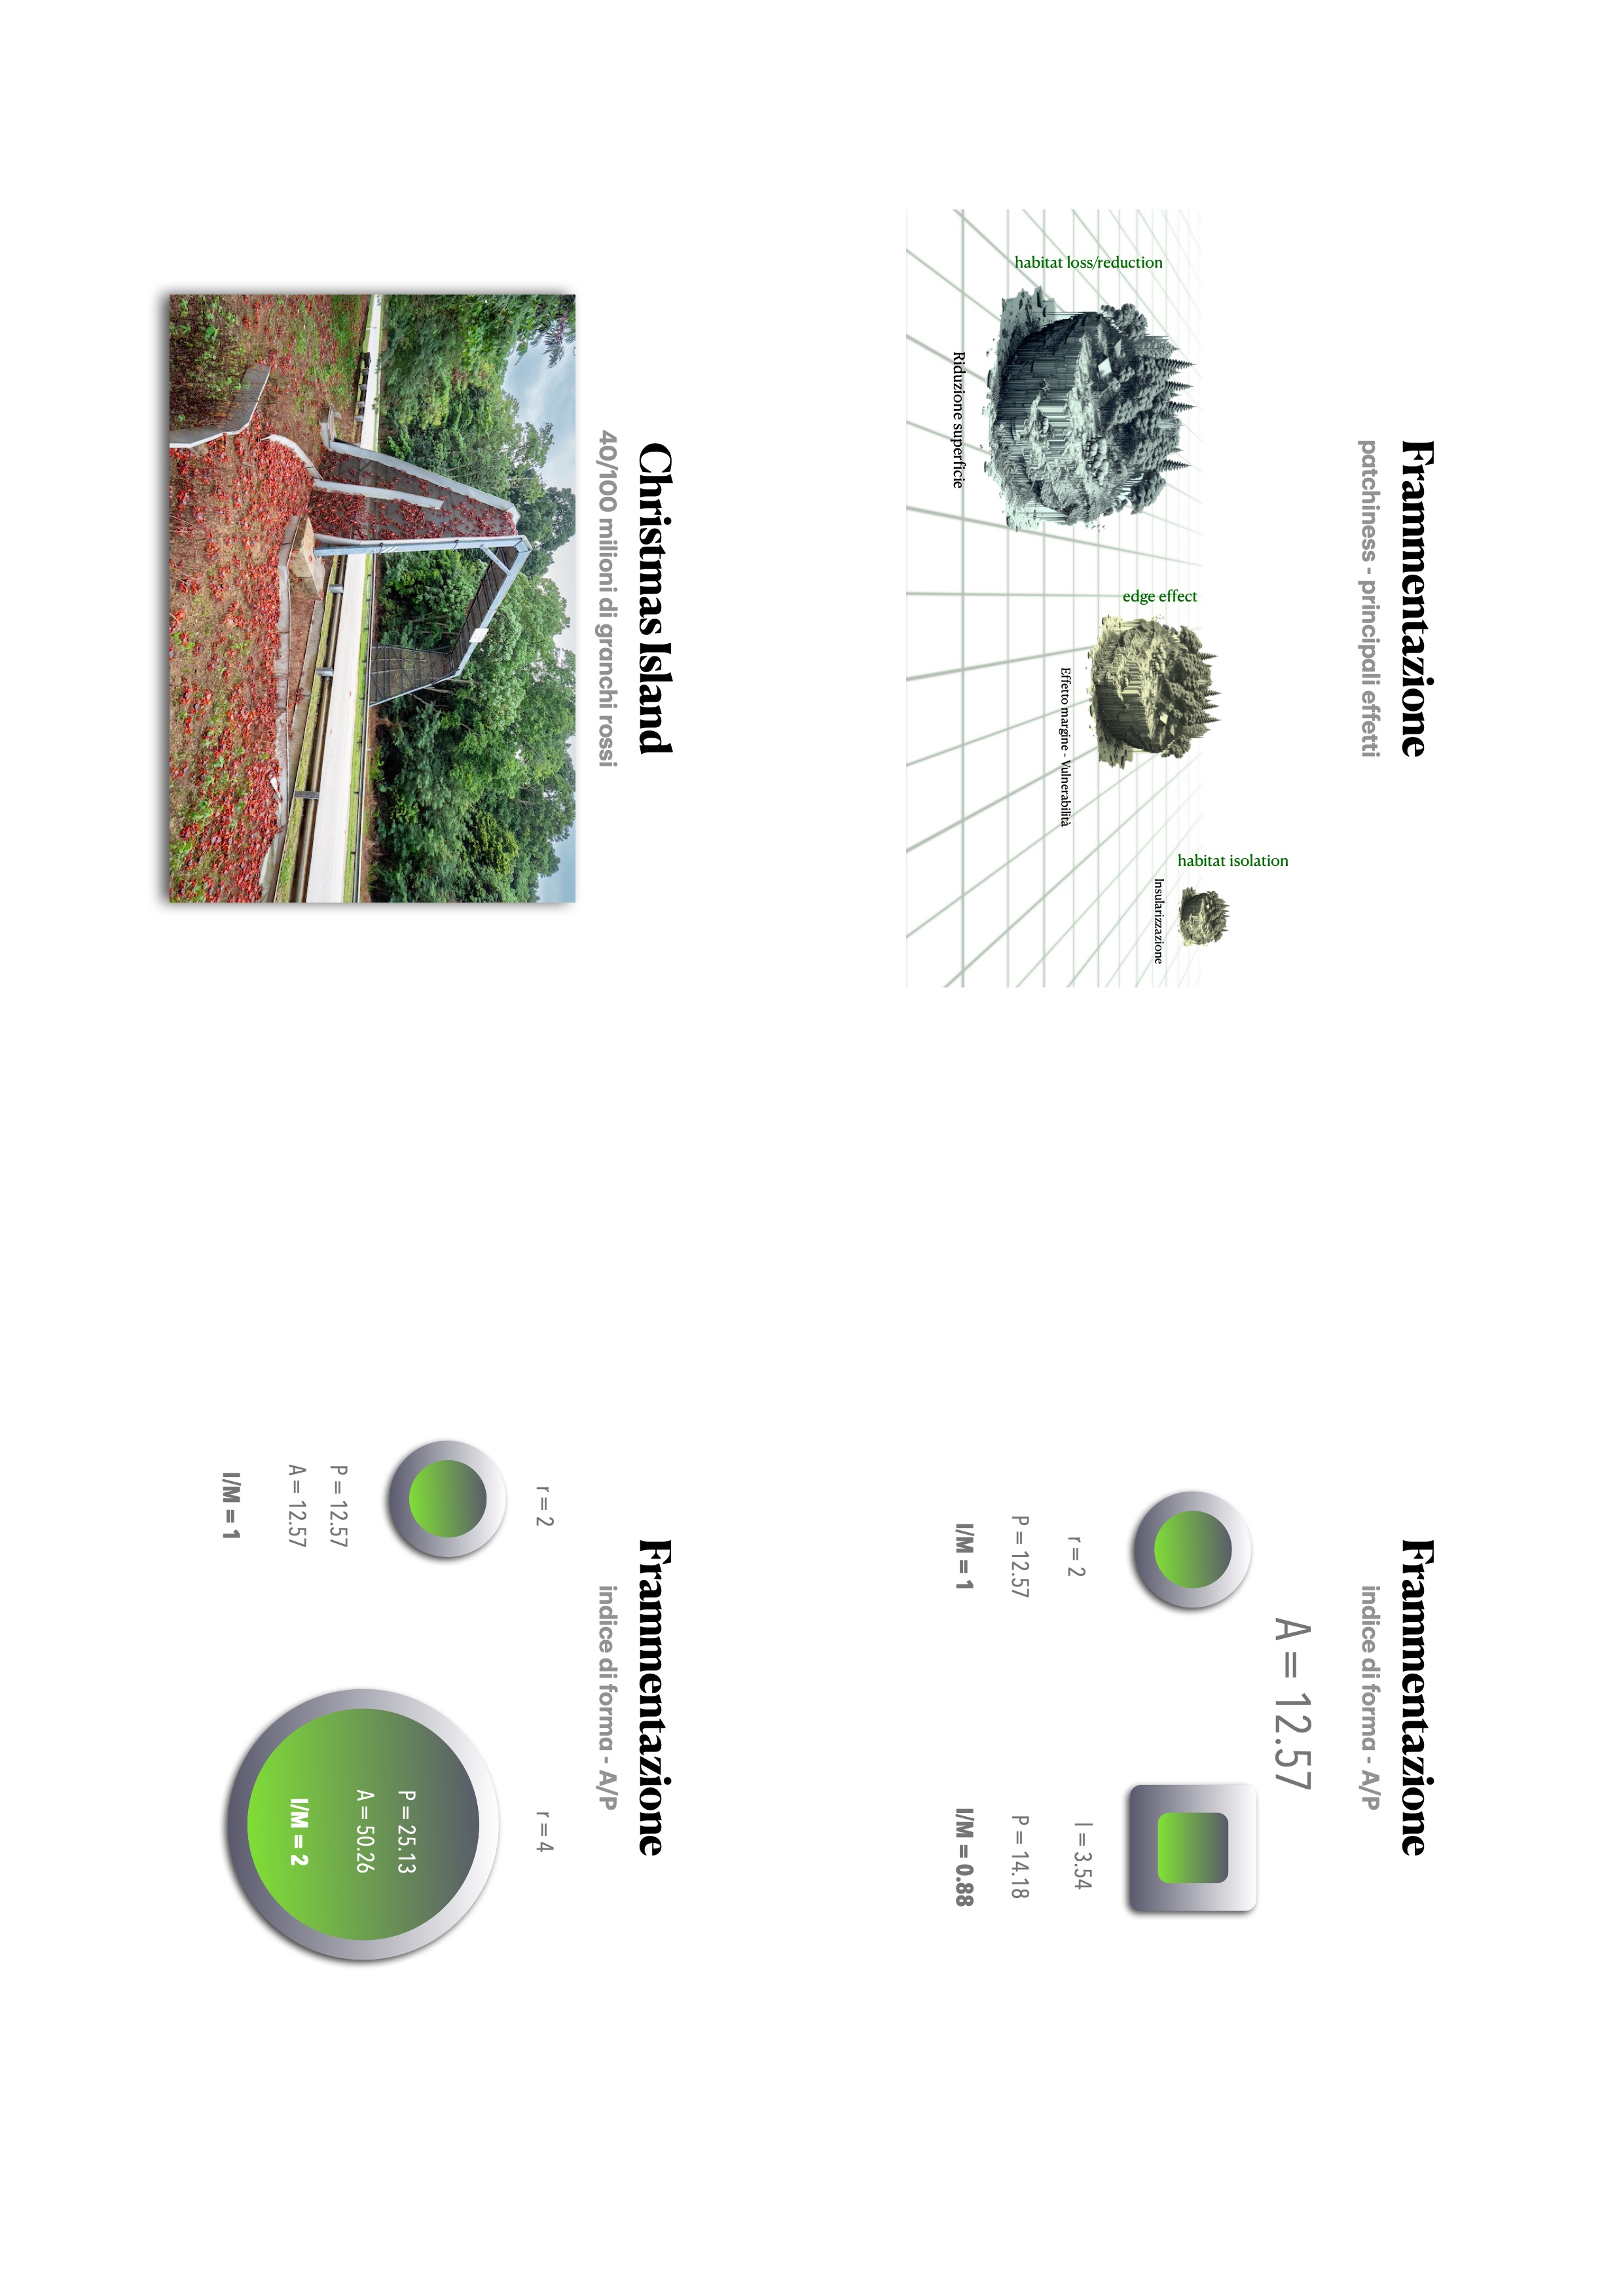
\includegraphics[keepaspectratio]{./figs/pctoREC/diversityRECSpoleto02 2-2.jpeg}}

\pandocbounded{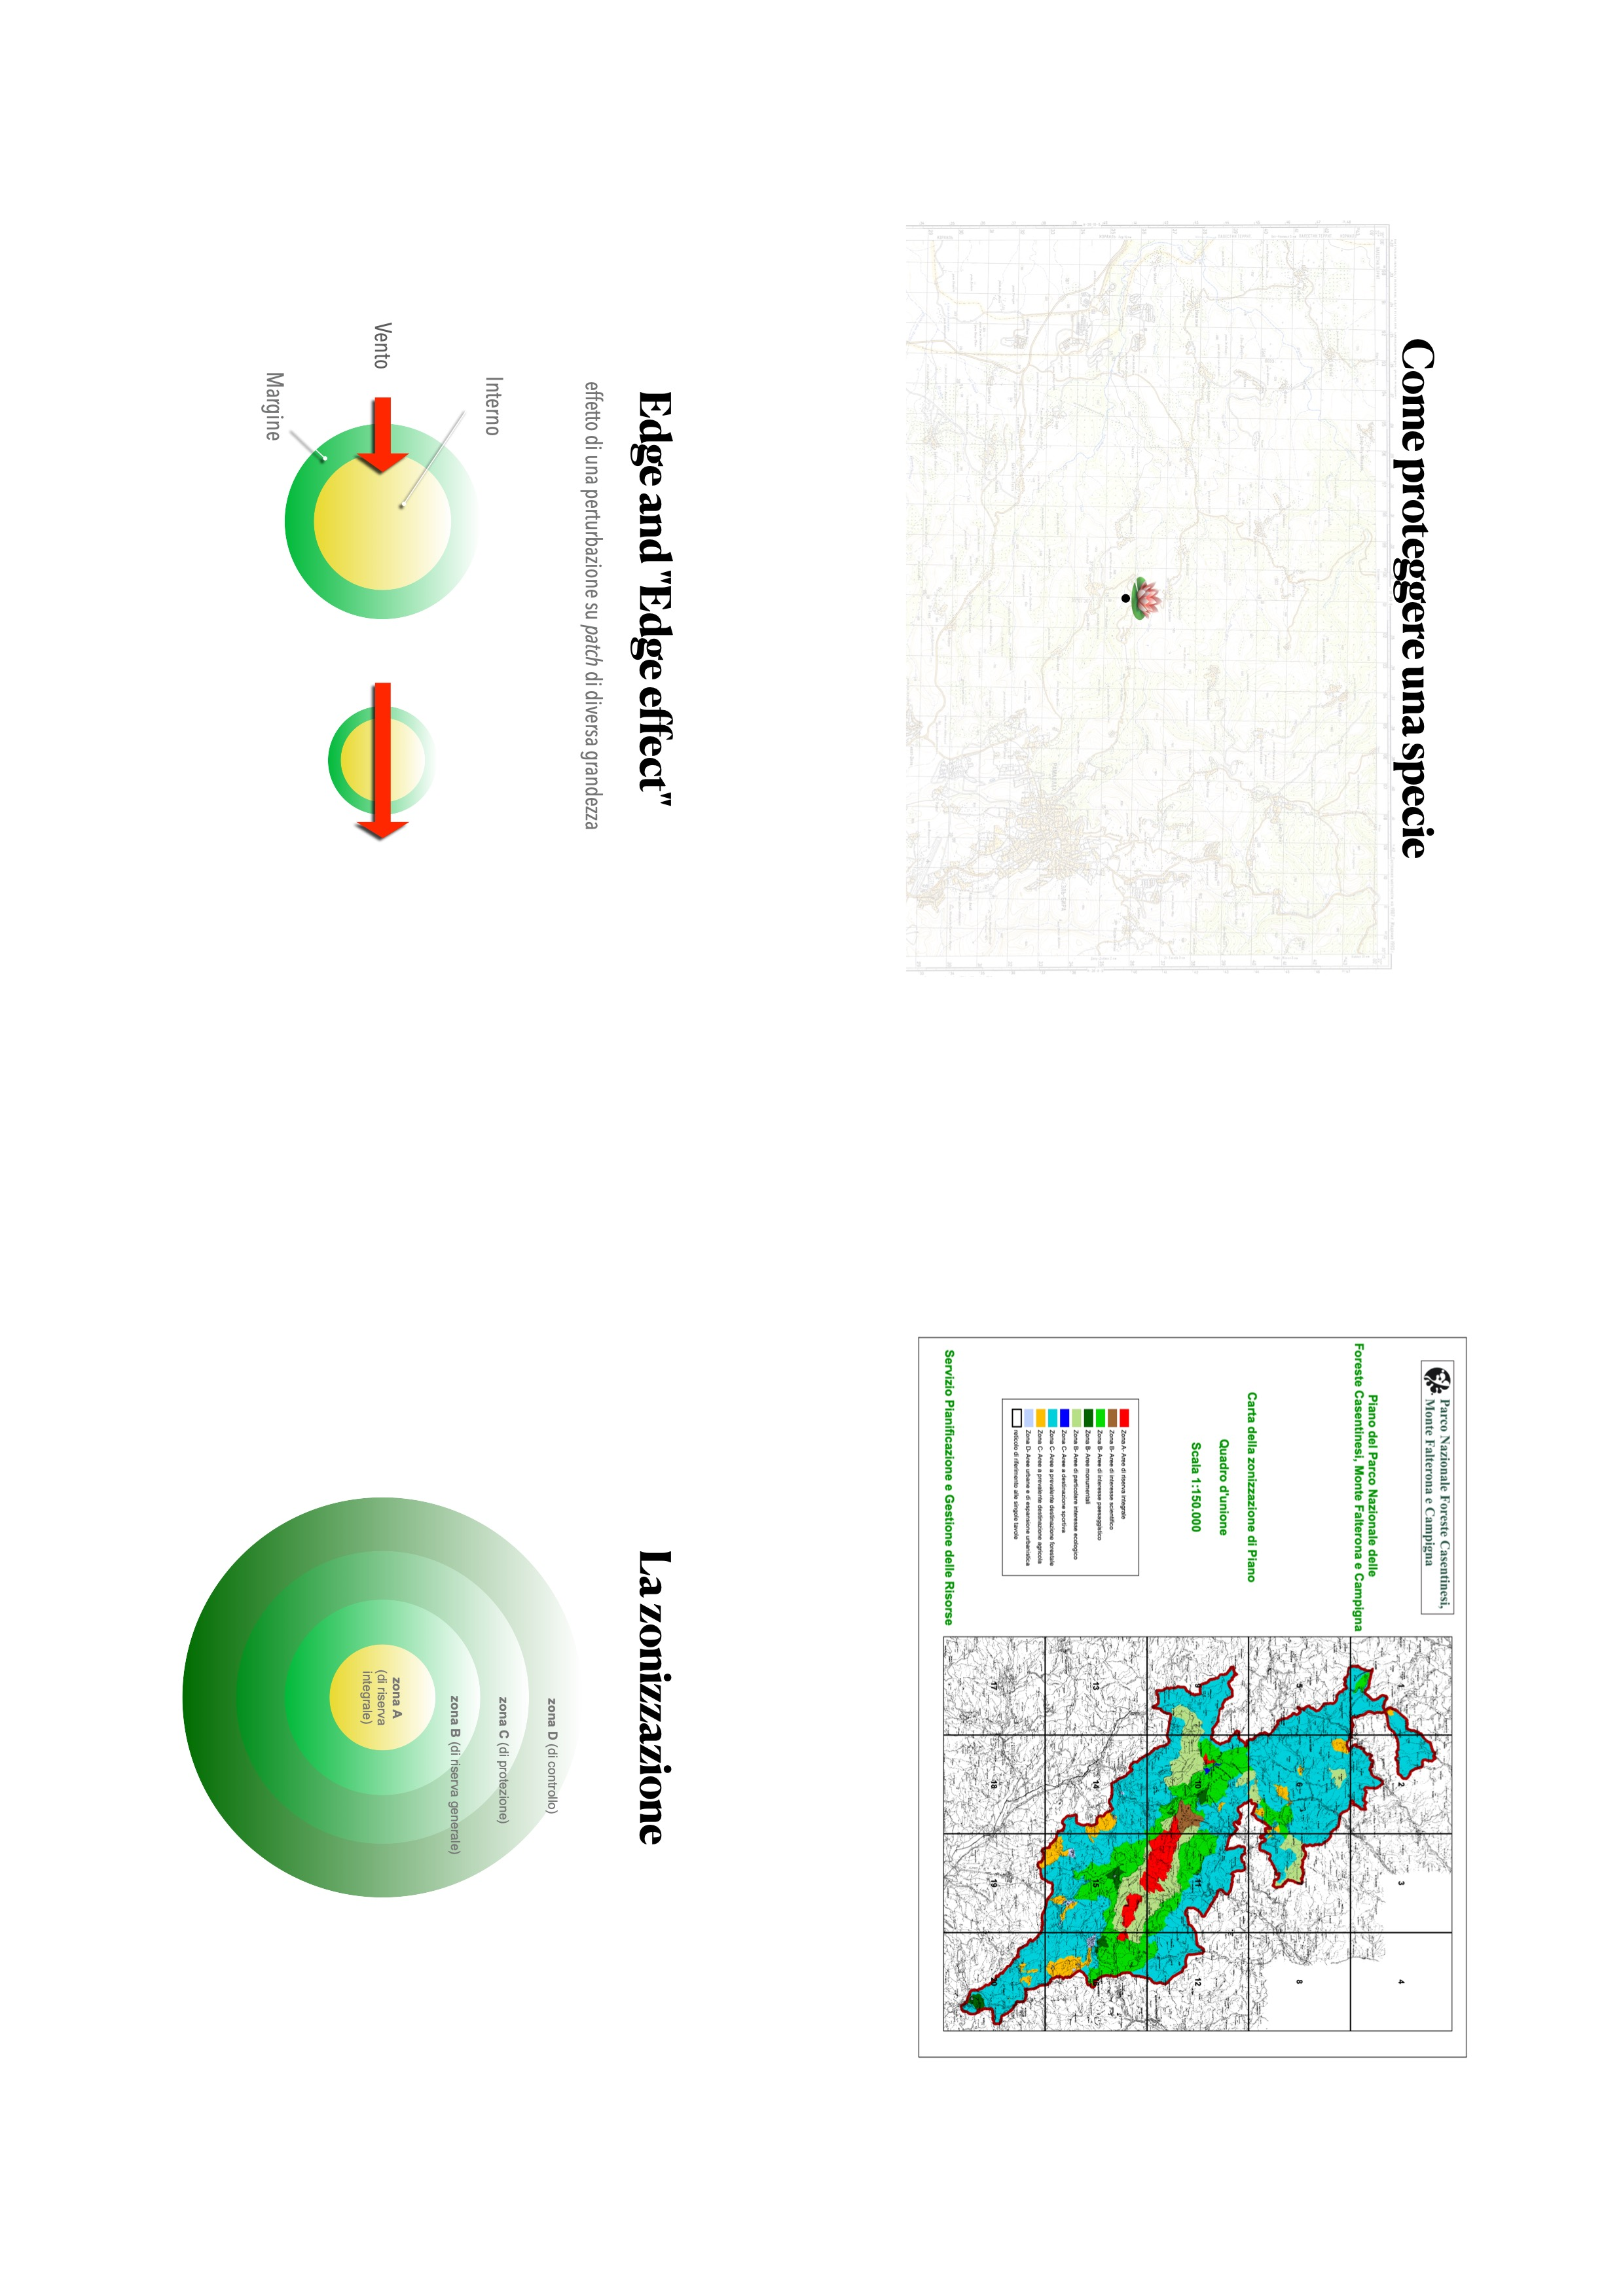
\includegraphics[keepaspectratio]{./figs/pctoREC/diversityRECSpoleto02 3-3.jpeg}}

\pandocbounded{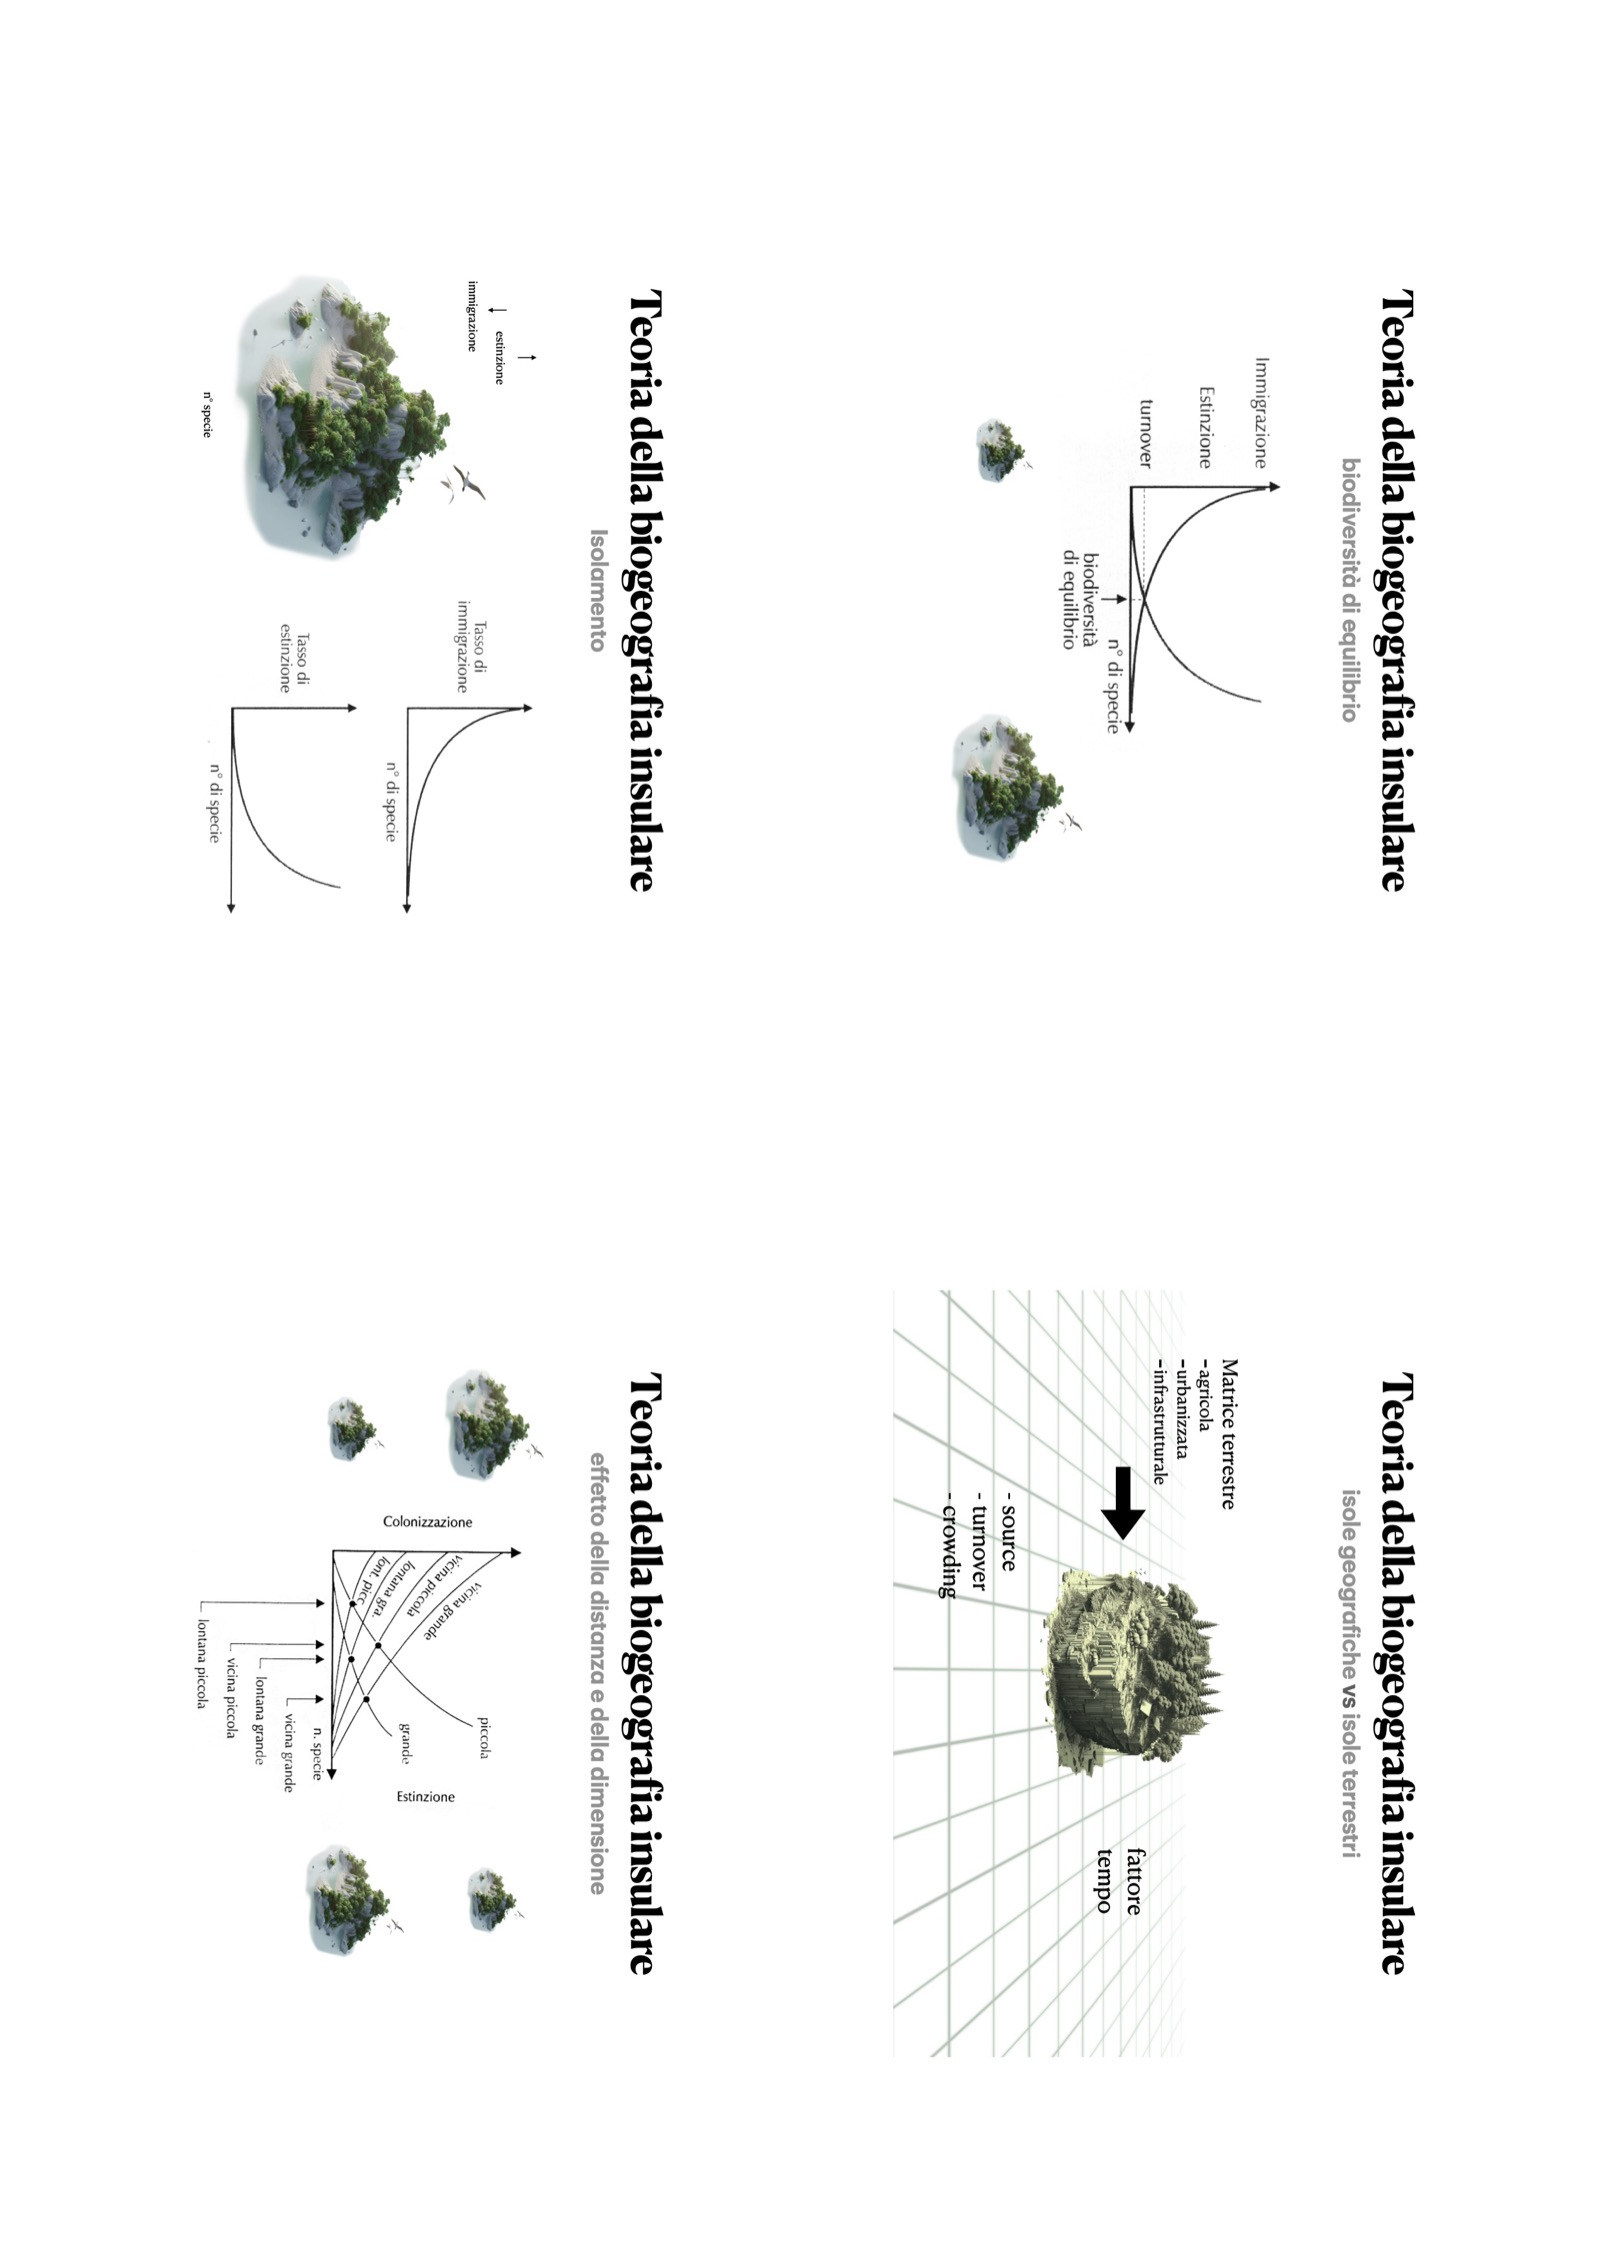
\includegraphics[keepaspectratio]{./figs/pctoREC/diversityRECSpoleto02 4-4.jpeg}}

\pandocbounded{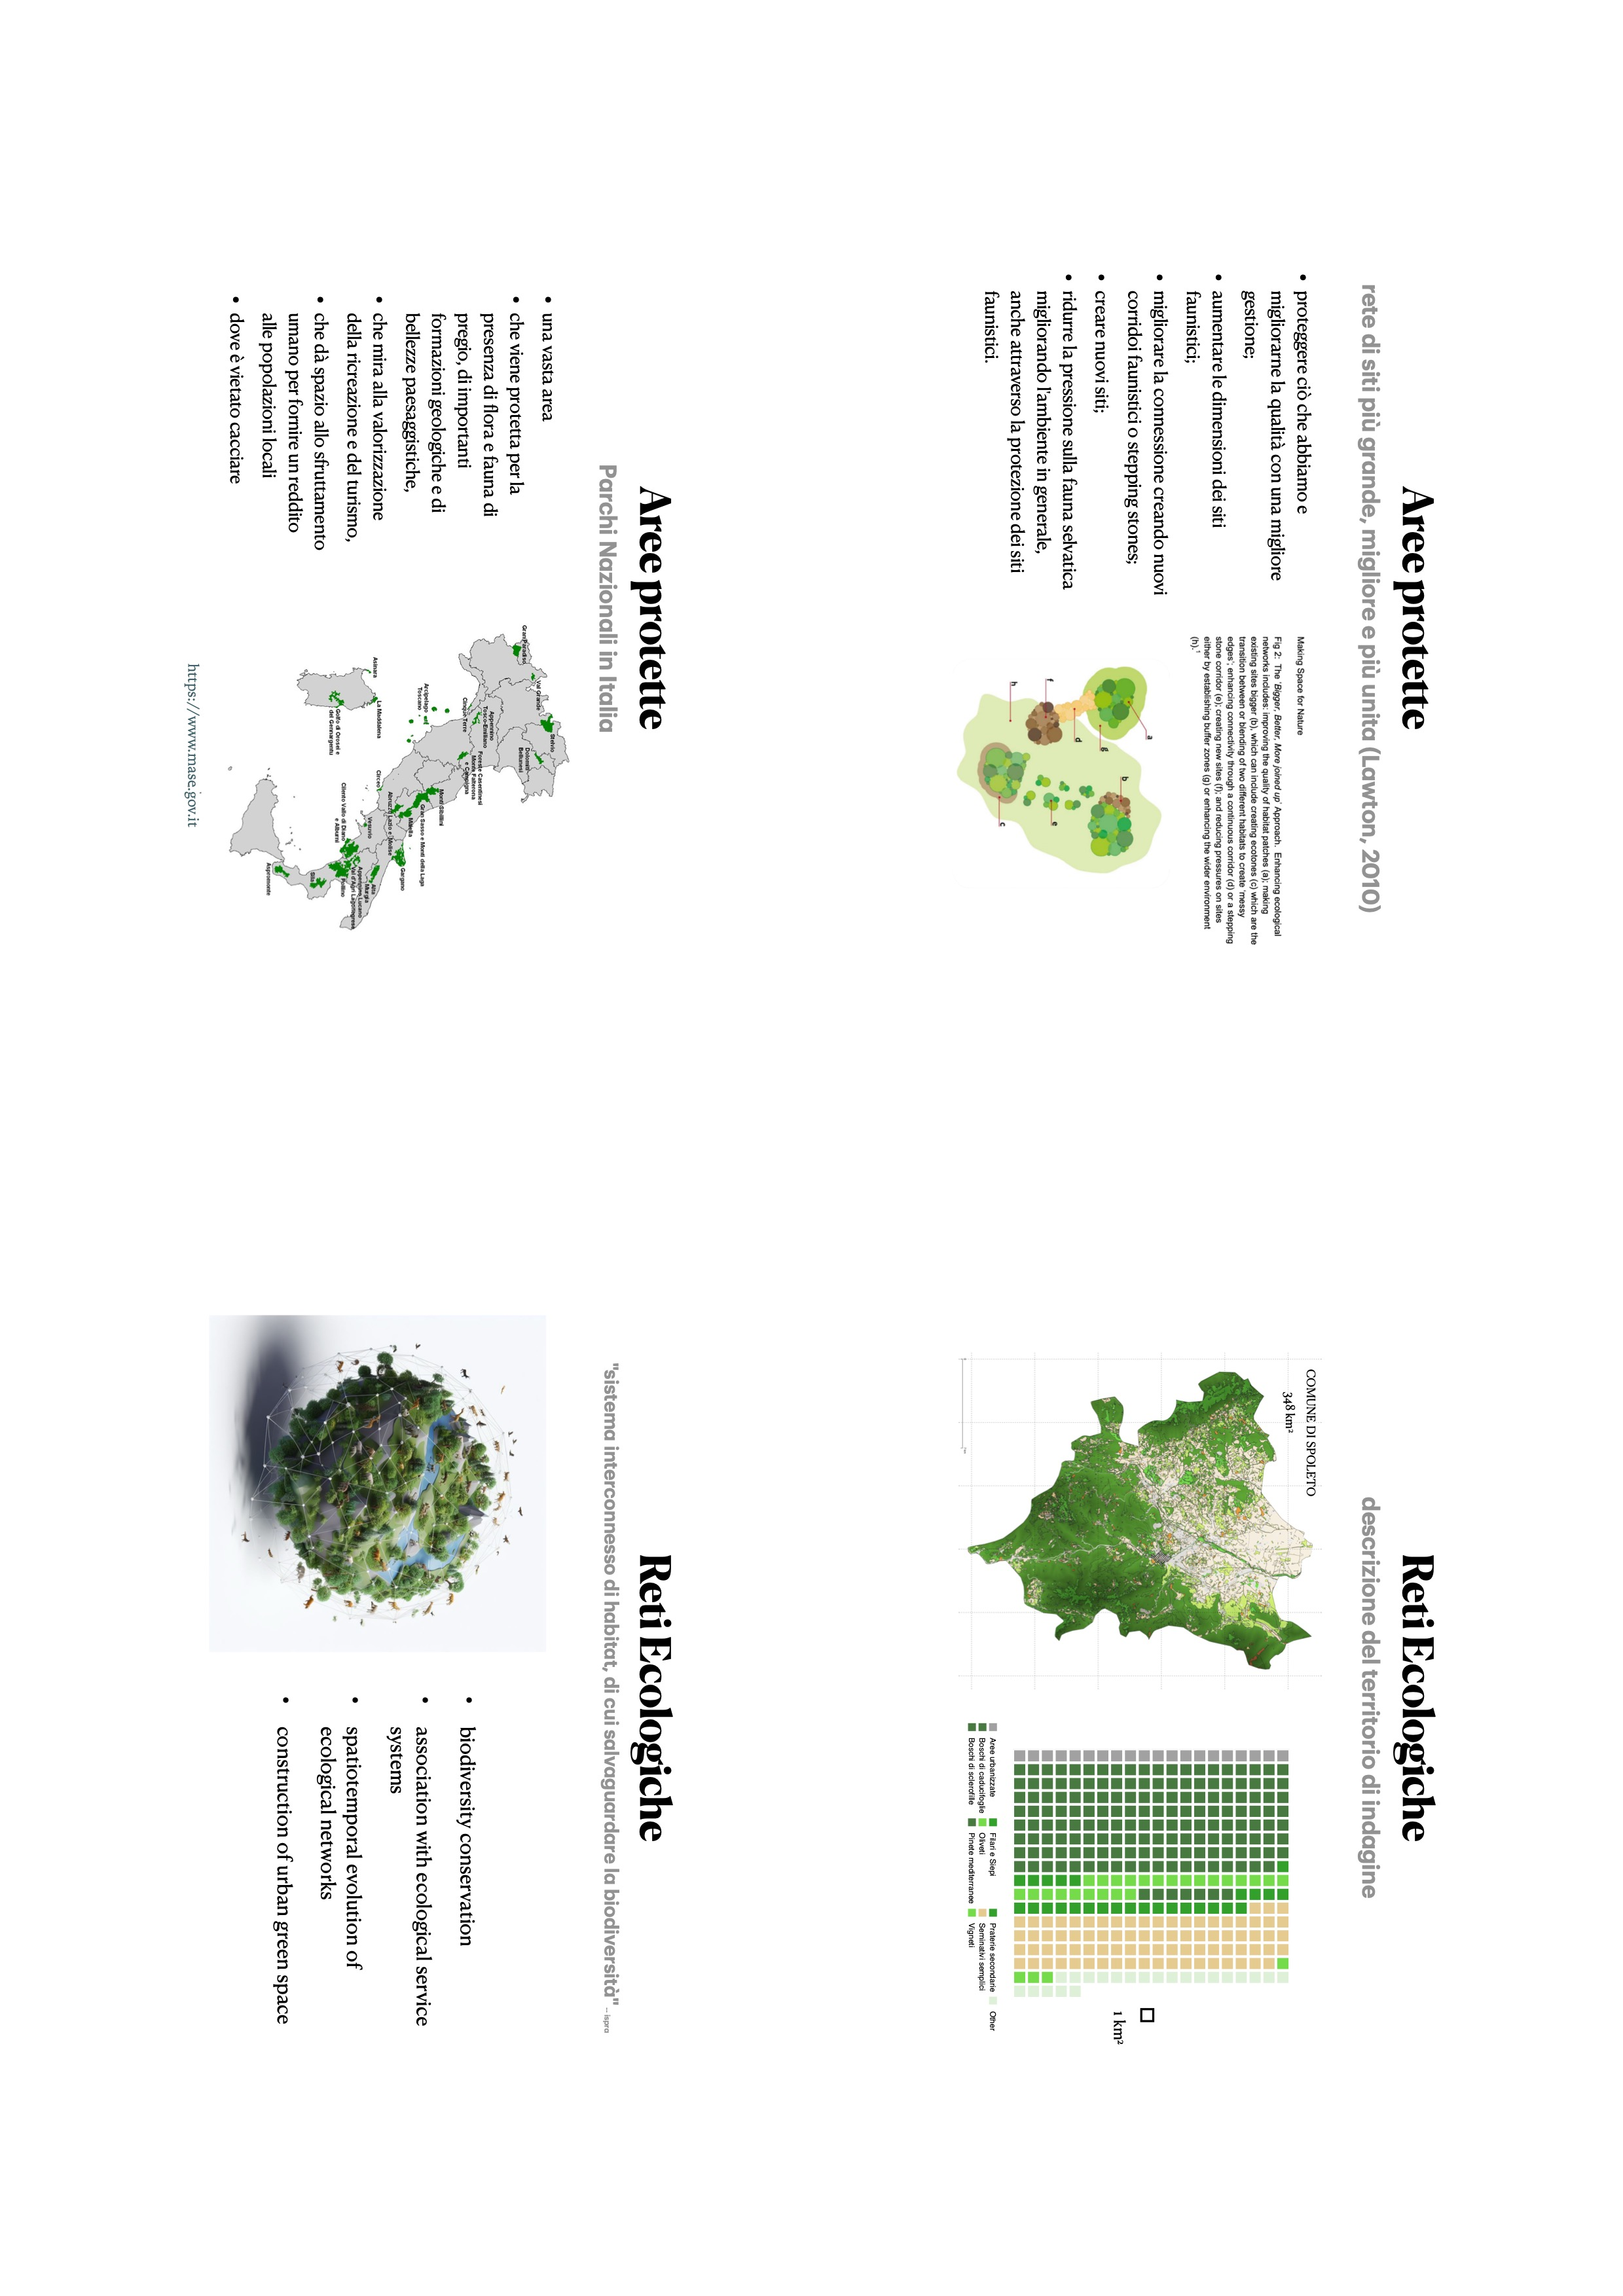
\includegraphics[keepaspectratio]{./figs/pctoREC/diversityRECSpoleto02 5-5.jpeg}}

\pandocbounded{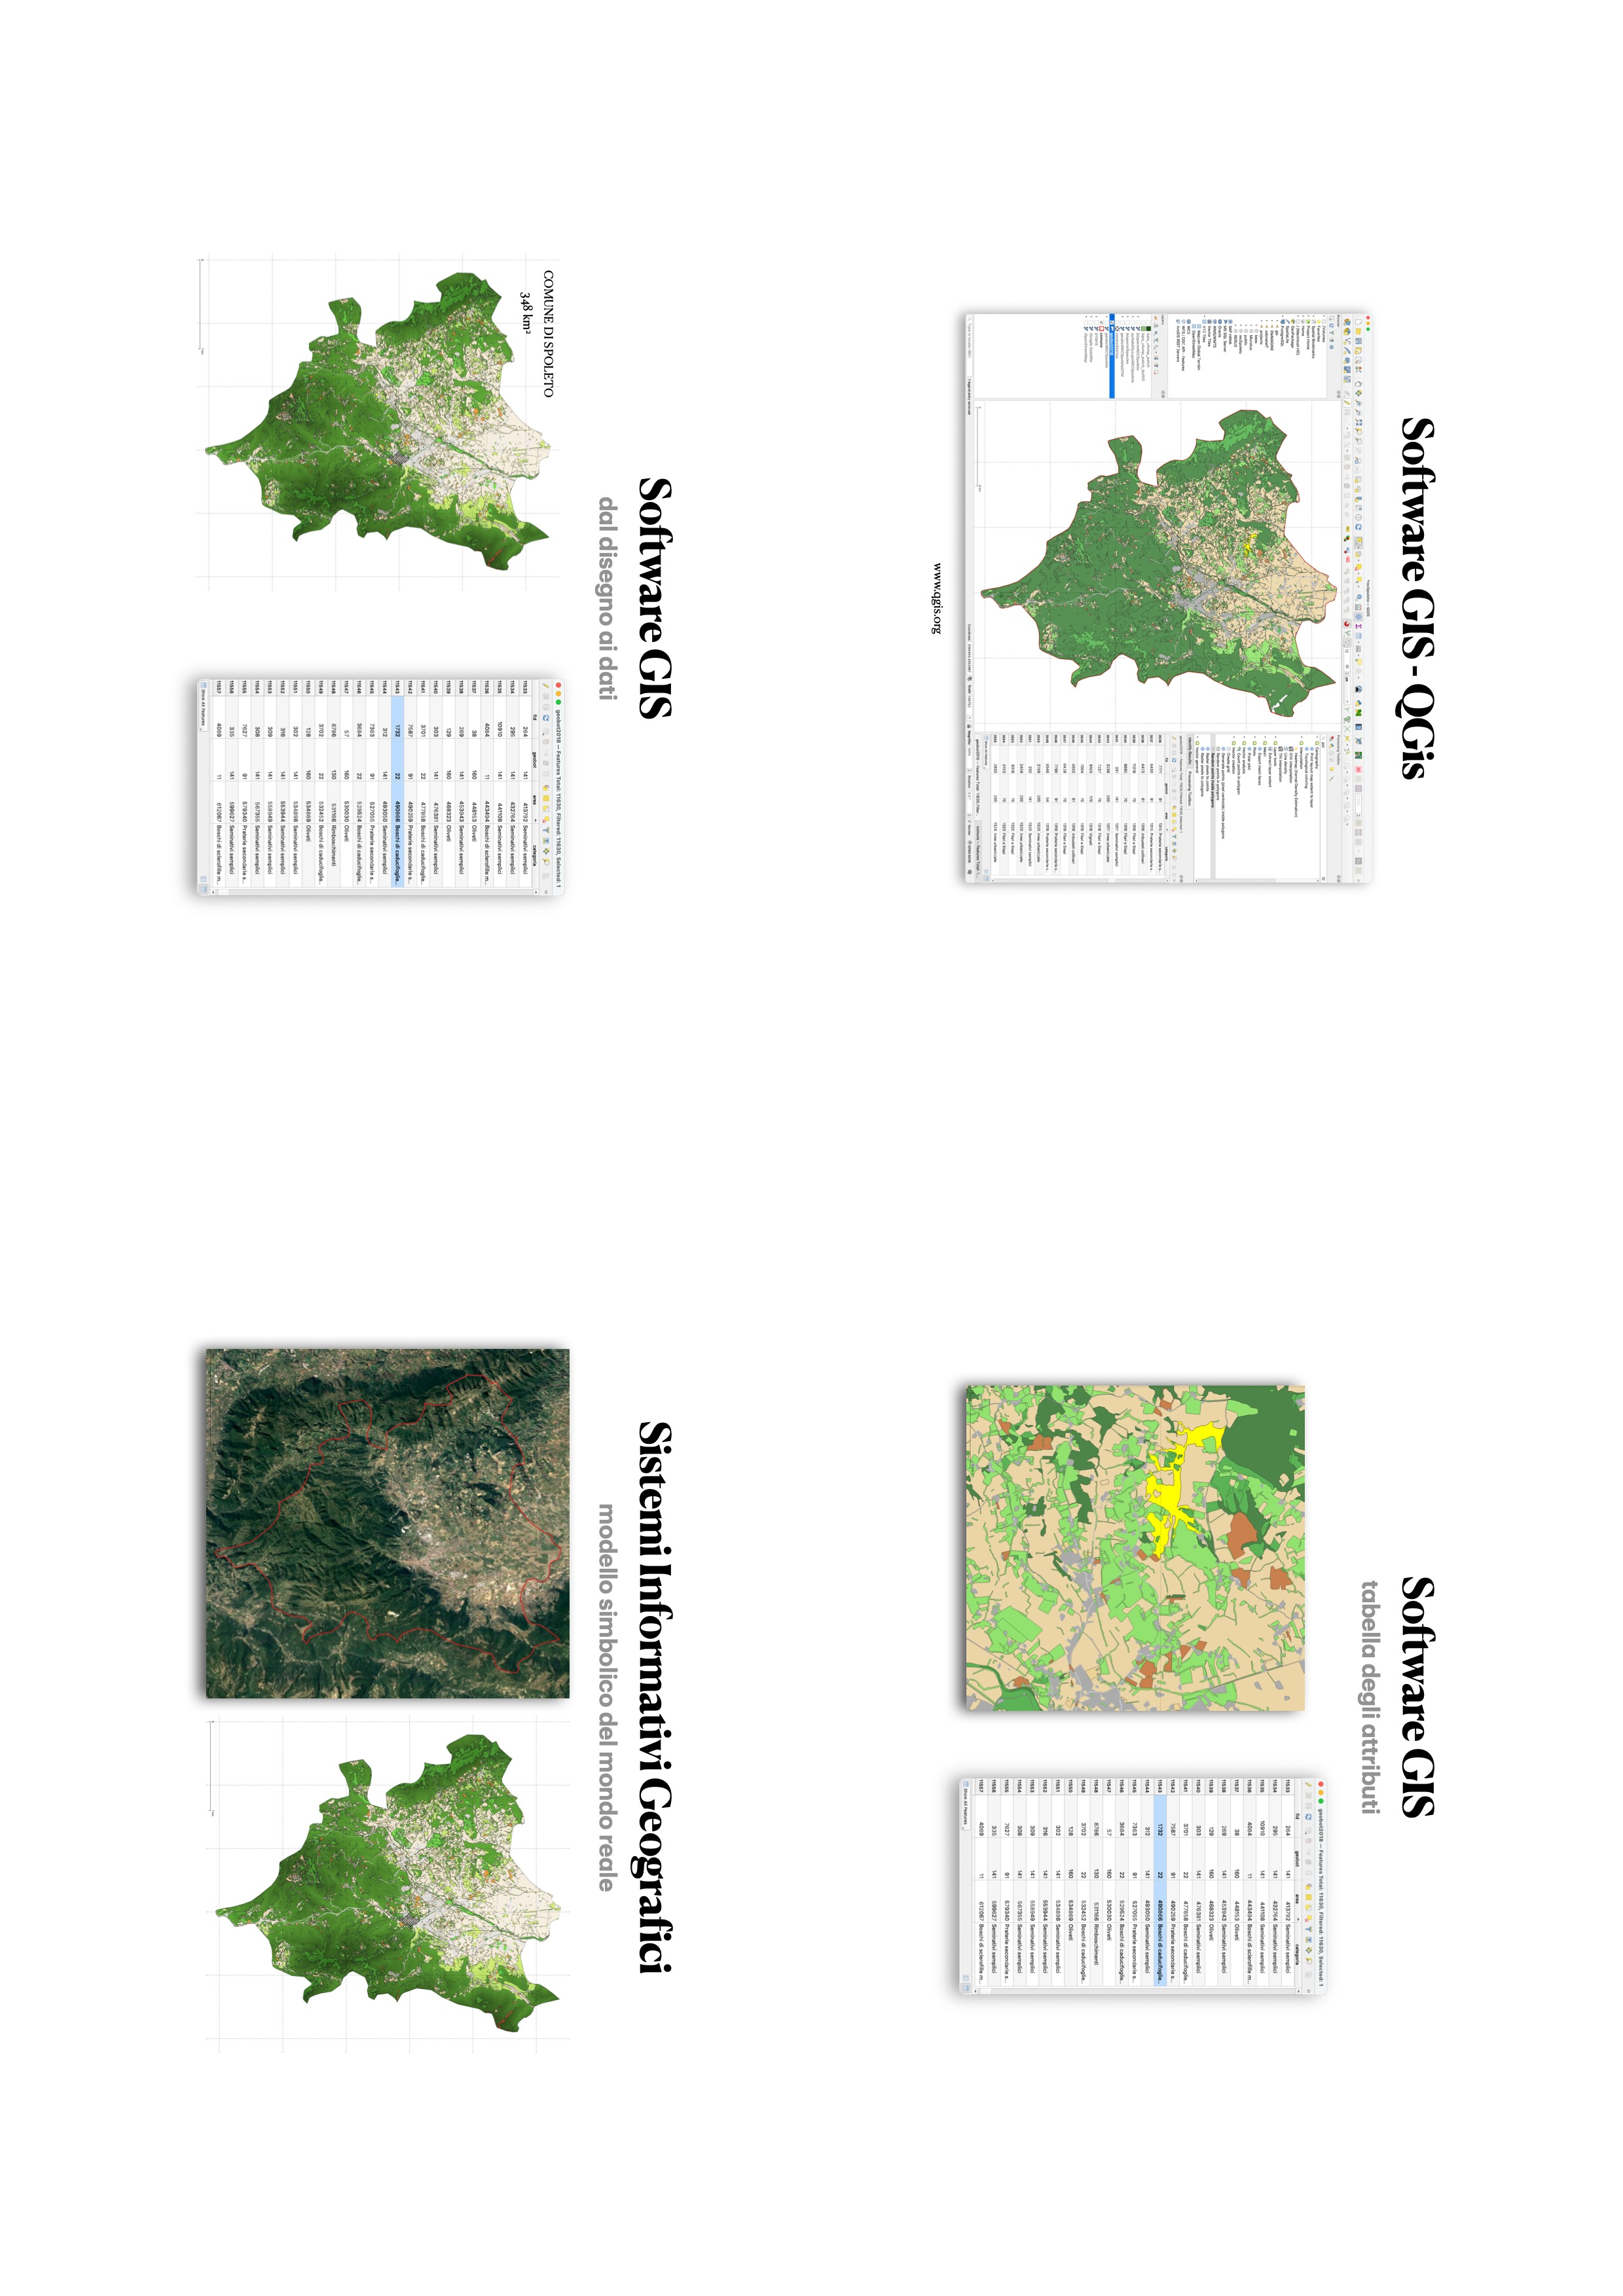
\includegraphics[keepaspectratio]{./figs/pctoREC/diversityRECSpoleto02 6-6.jpeg}}

\pandocbounded{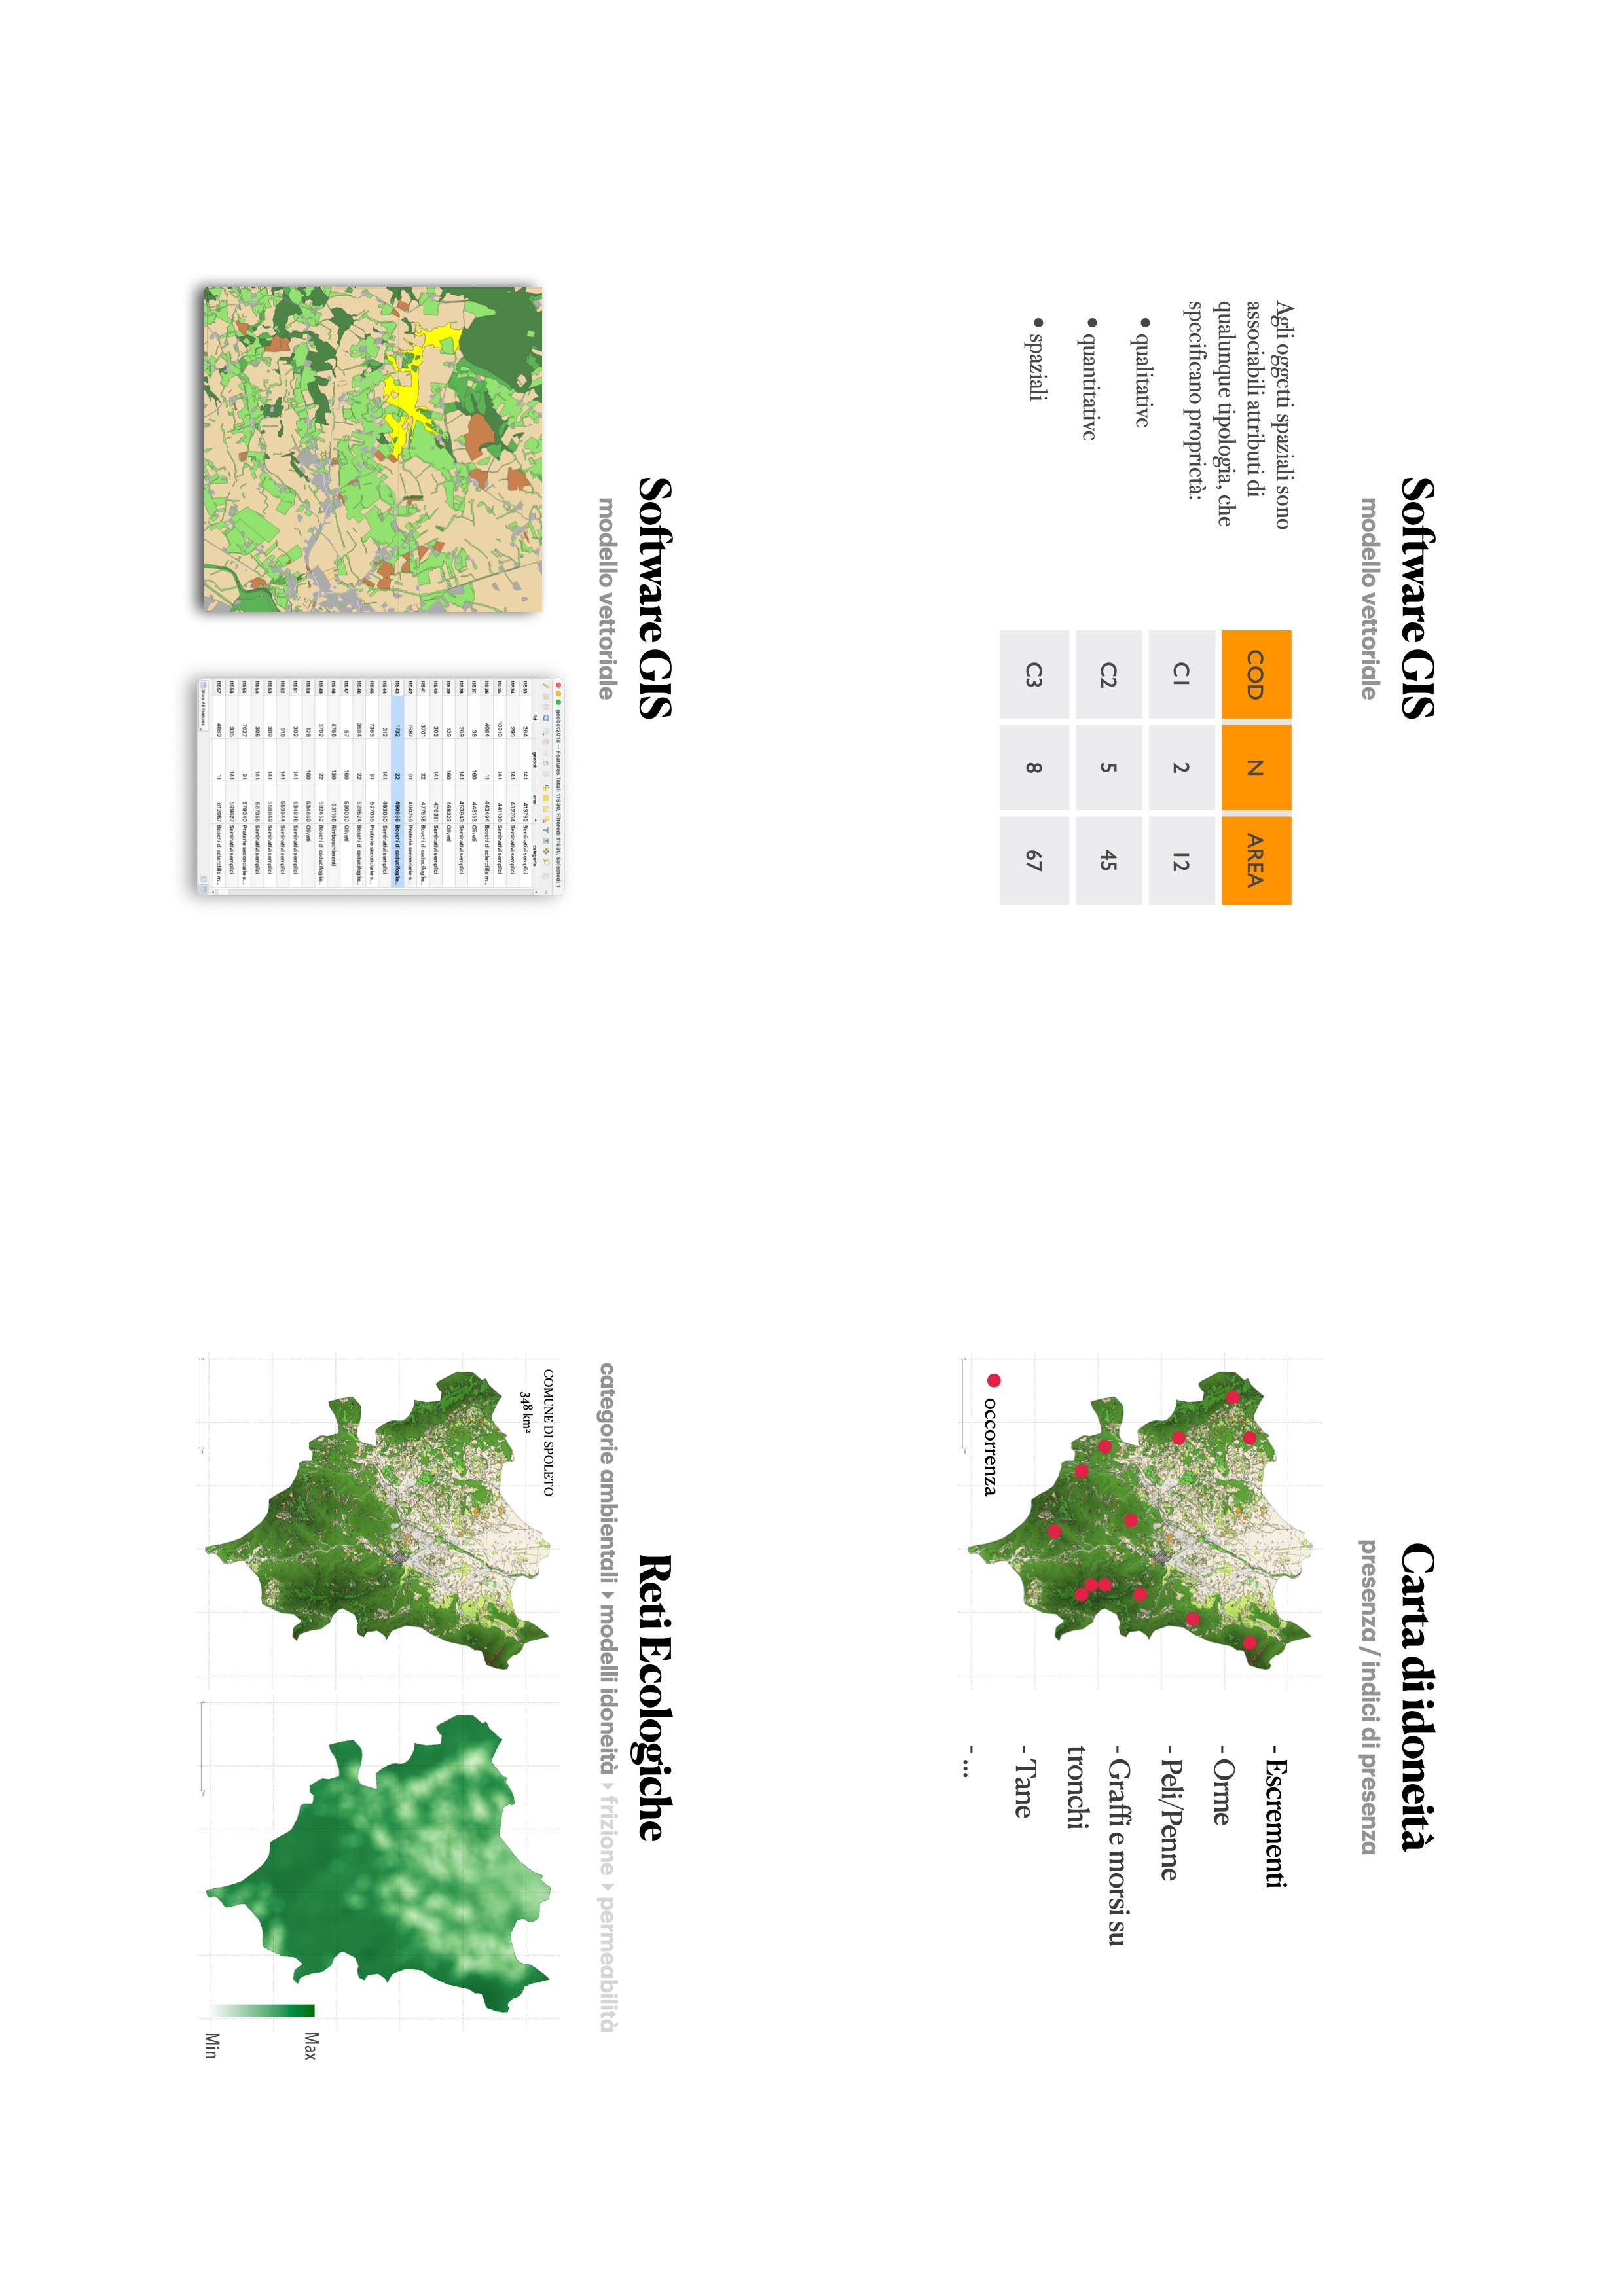
\includegraphics[keepaspectratio]{./figs/pctoREC/diversityRECSpoleto02 7-7.jpeg}}

\pandocbounded{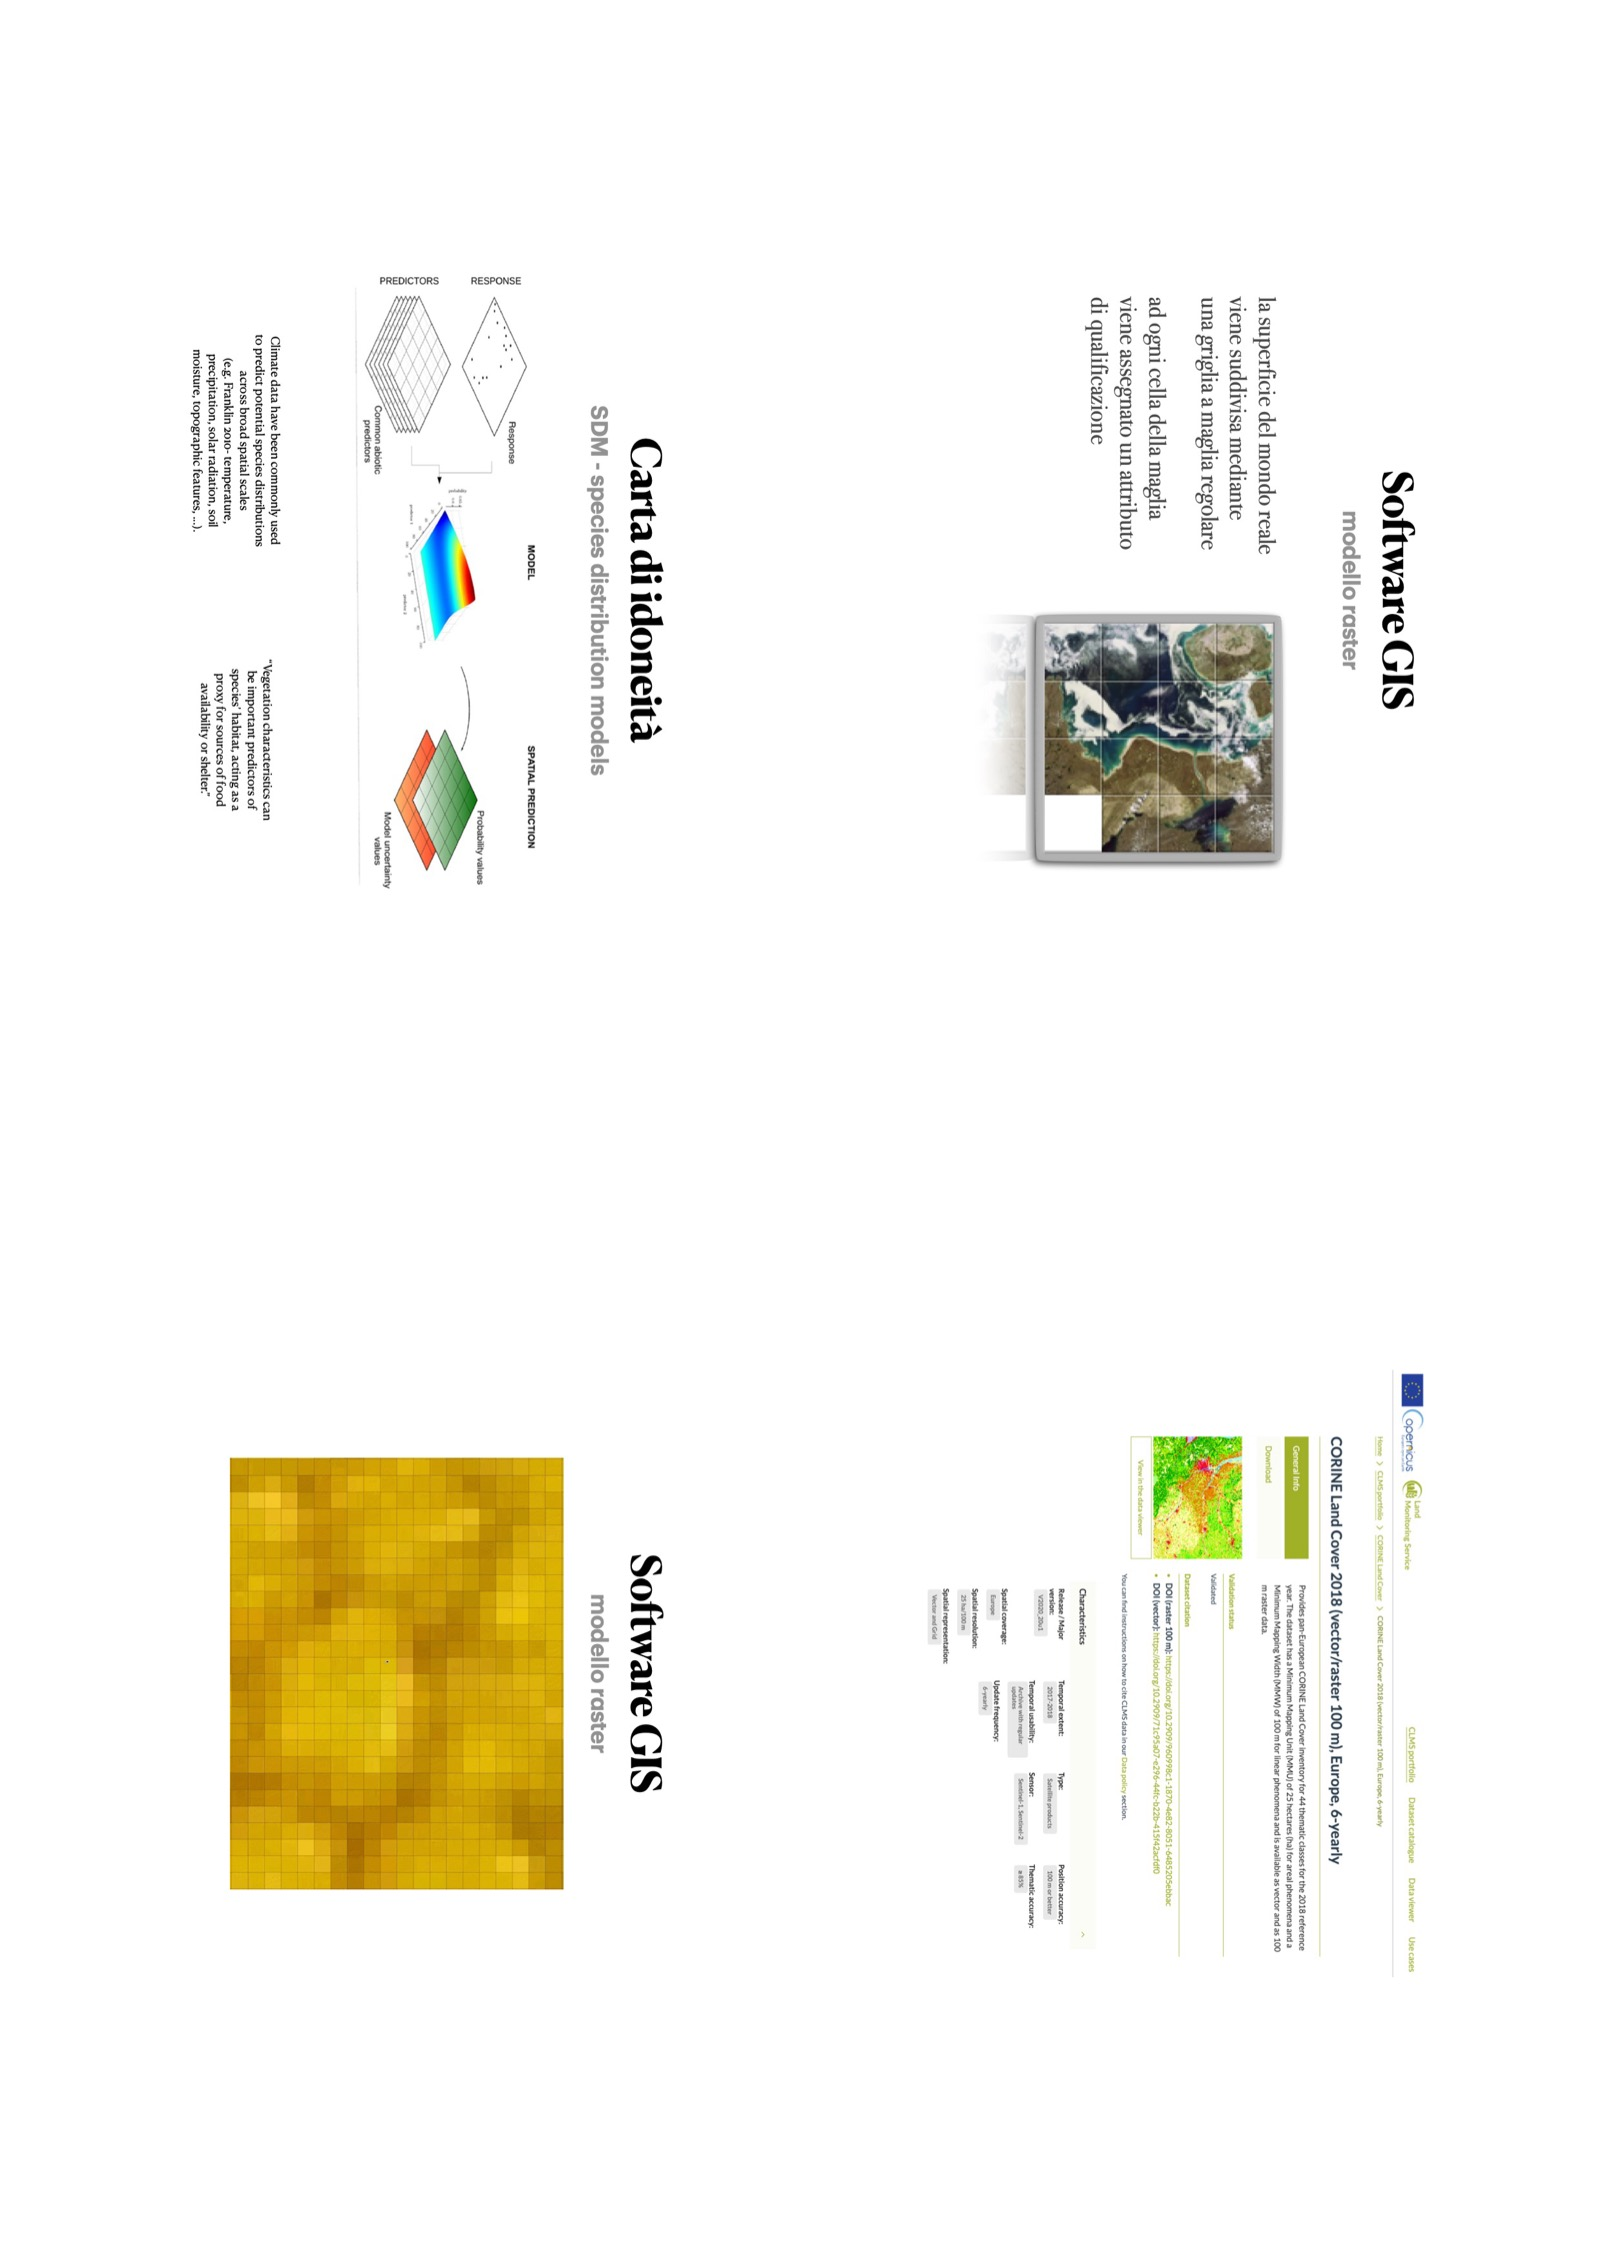
\includegraphics[keepaspectratio]{./figs/pctoREC/diversityRECSpoleto02 8-8.jpeg}}

\pandocbounded{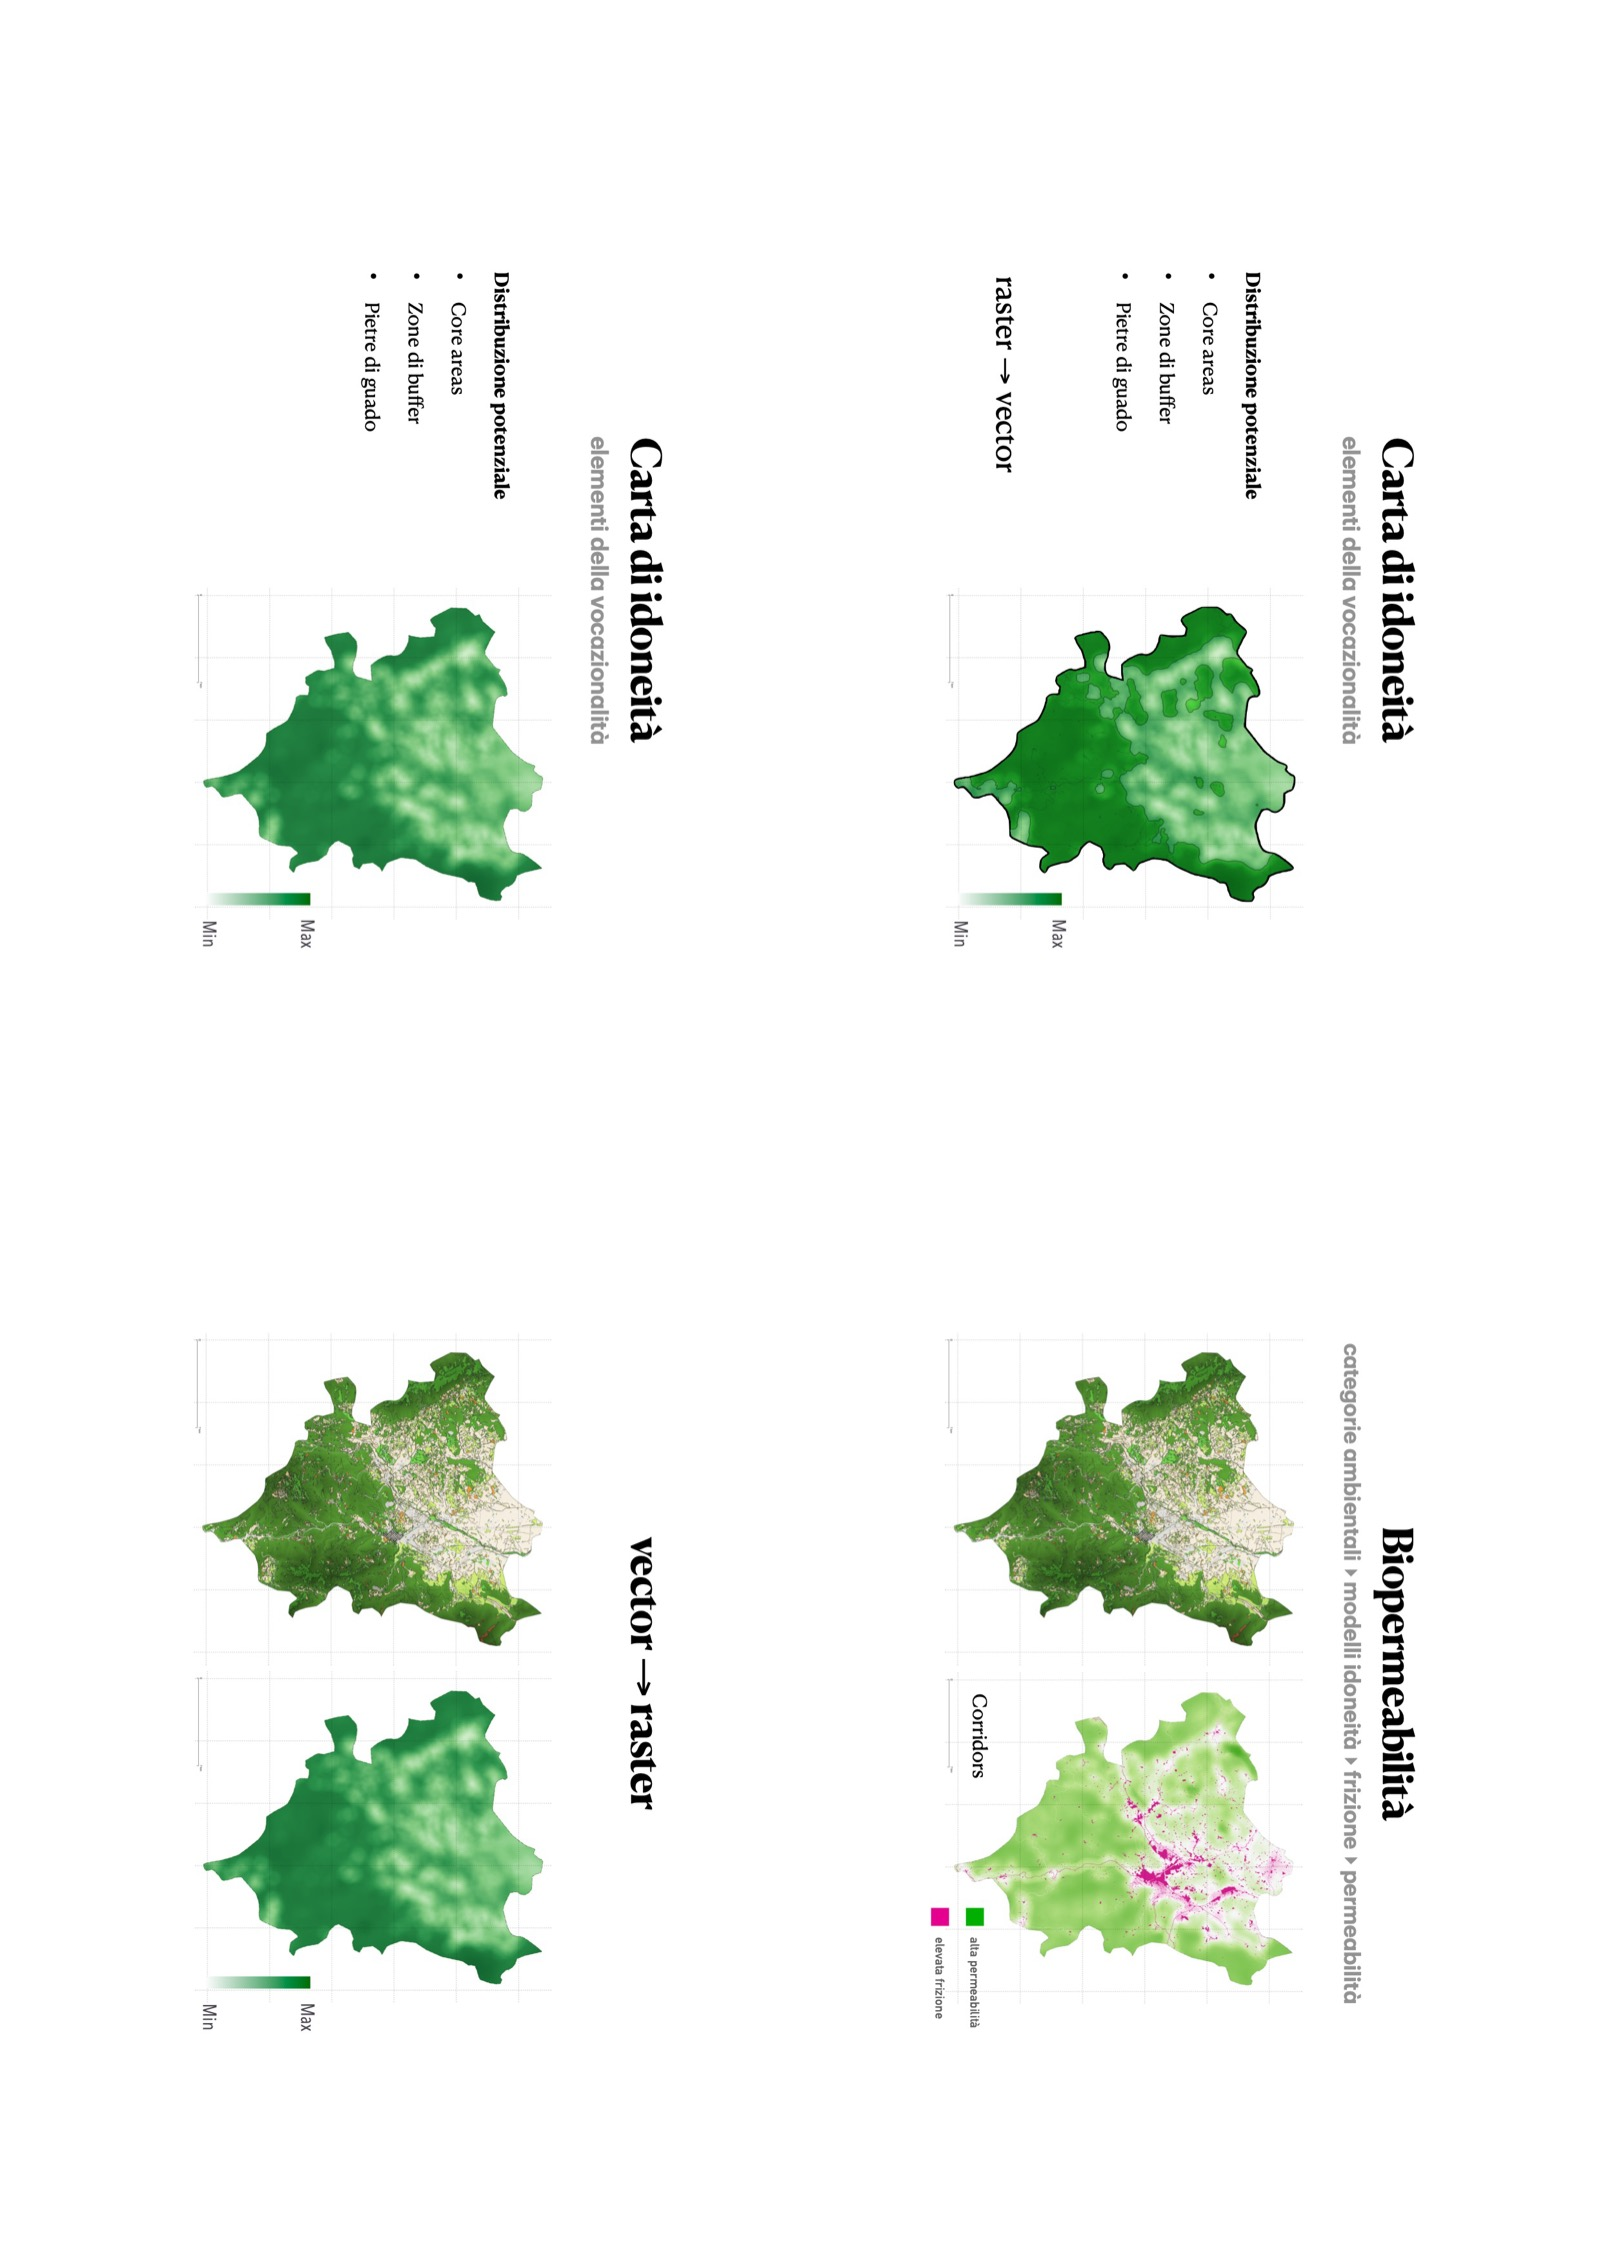
\includegraphics[keepaspectratio]{./figs/pctoREC/diversityRECSpoleto02 9-9.jpeg}}

\pandocbounded{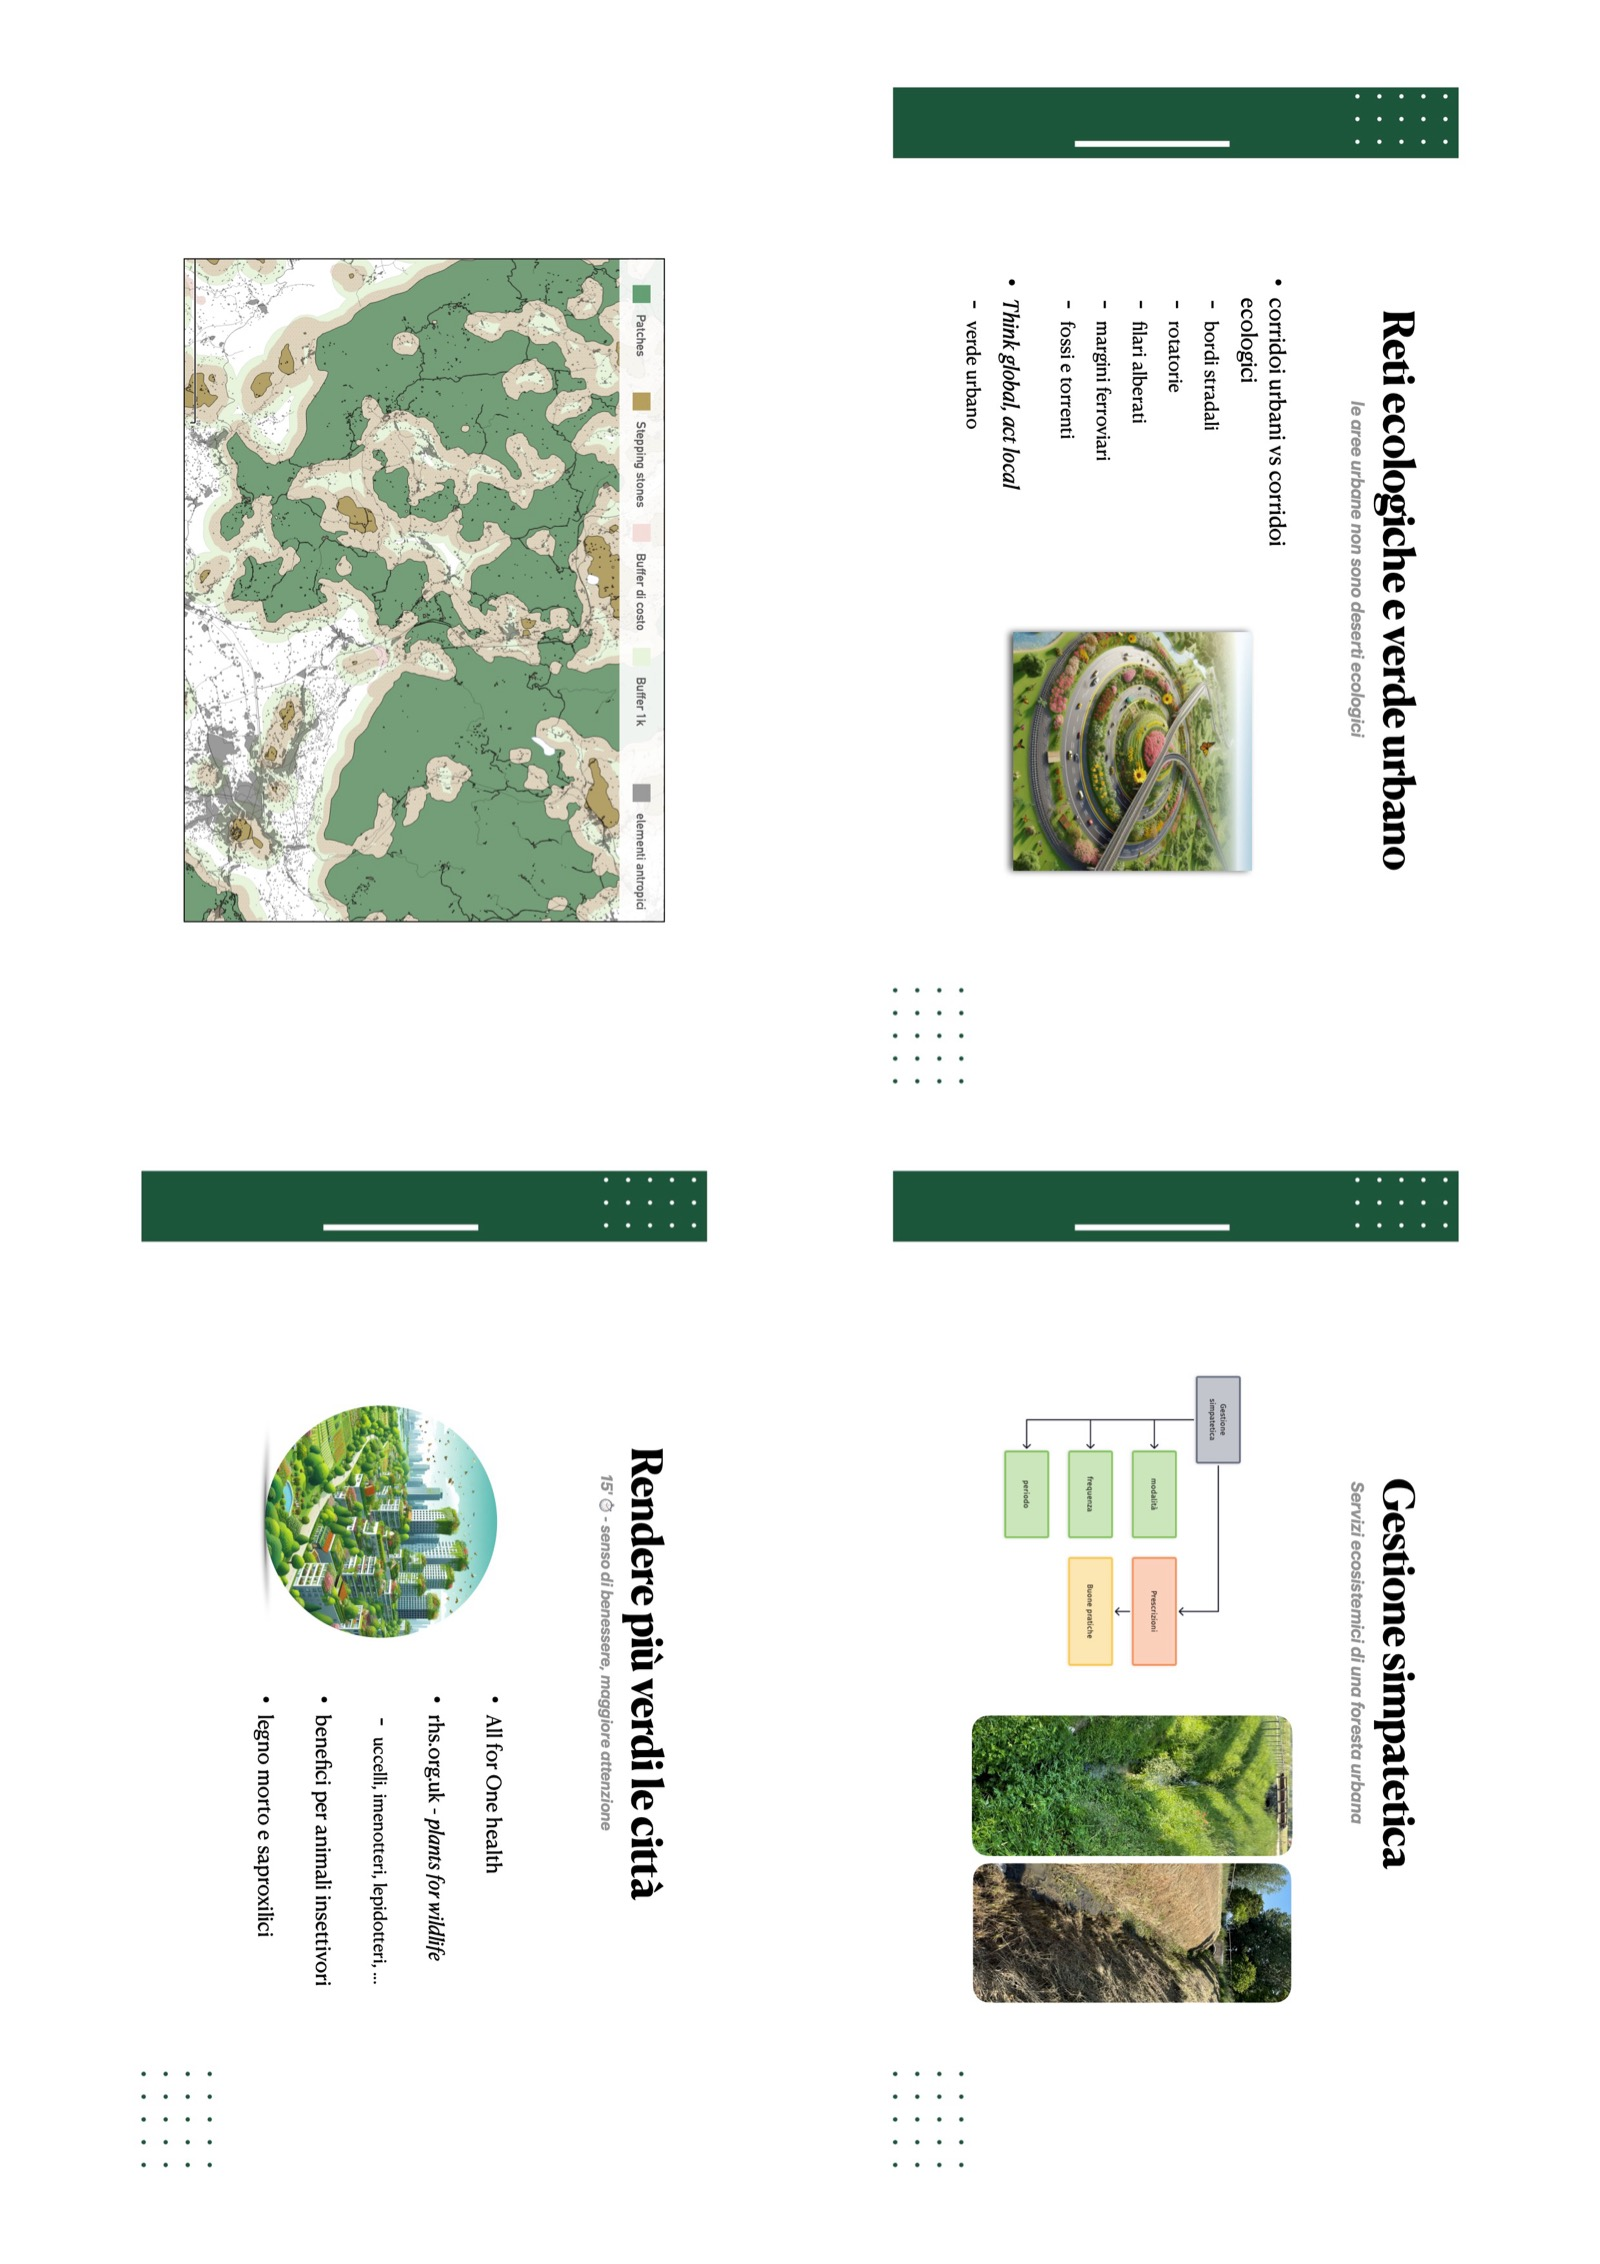
\includegraphics[keepaspectratio]{./figs/pctoREC/diversityRECSpoleto02 10-10.jpeg}}

\pandocbounded{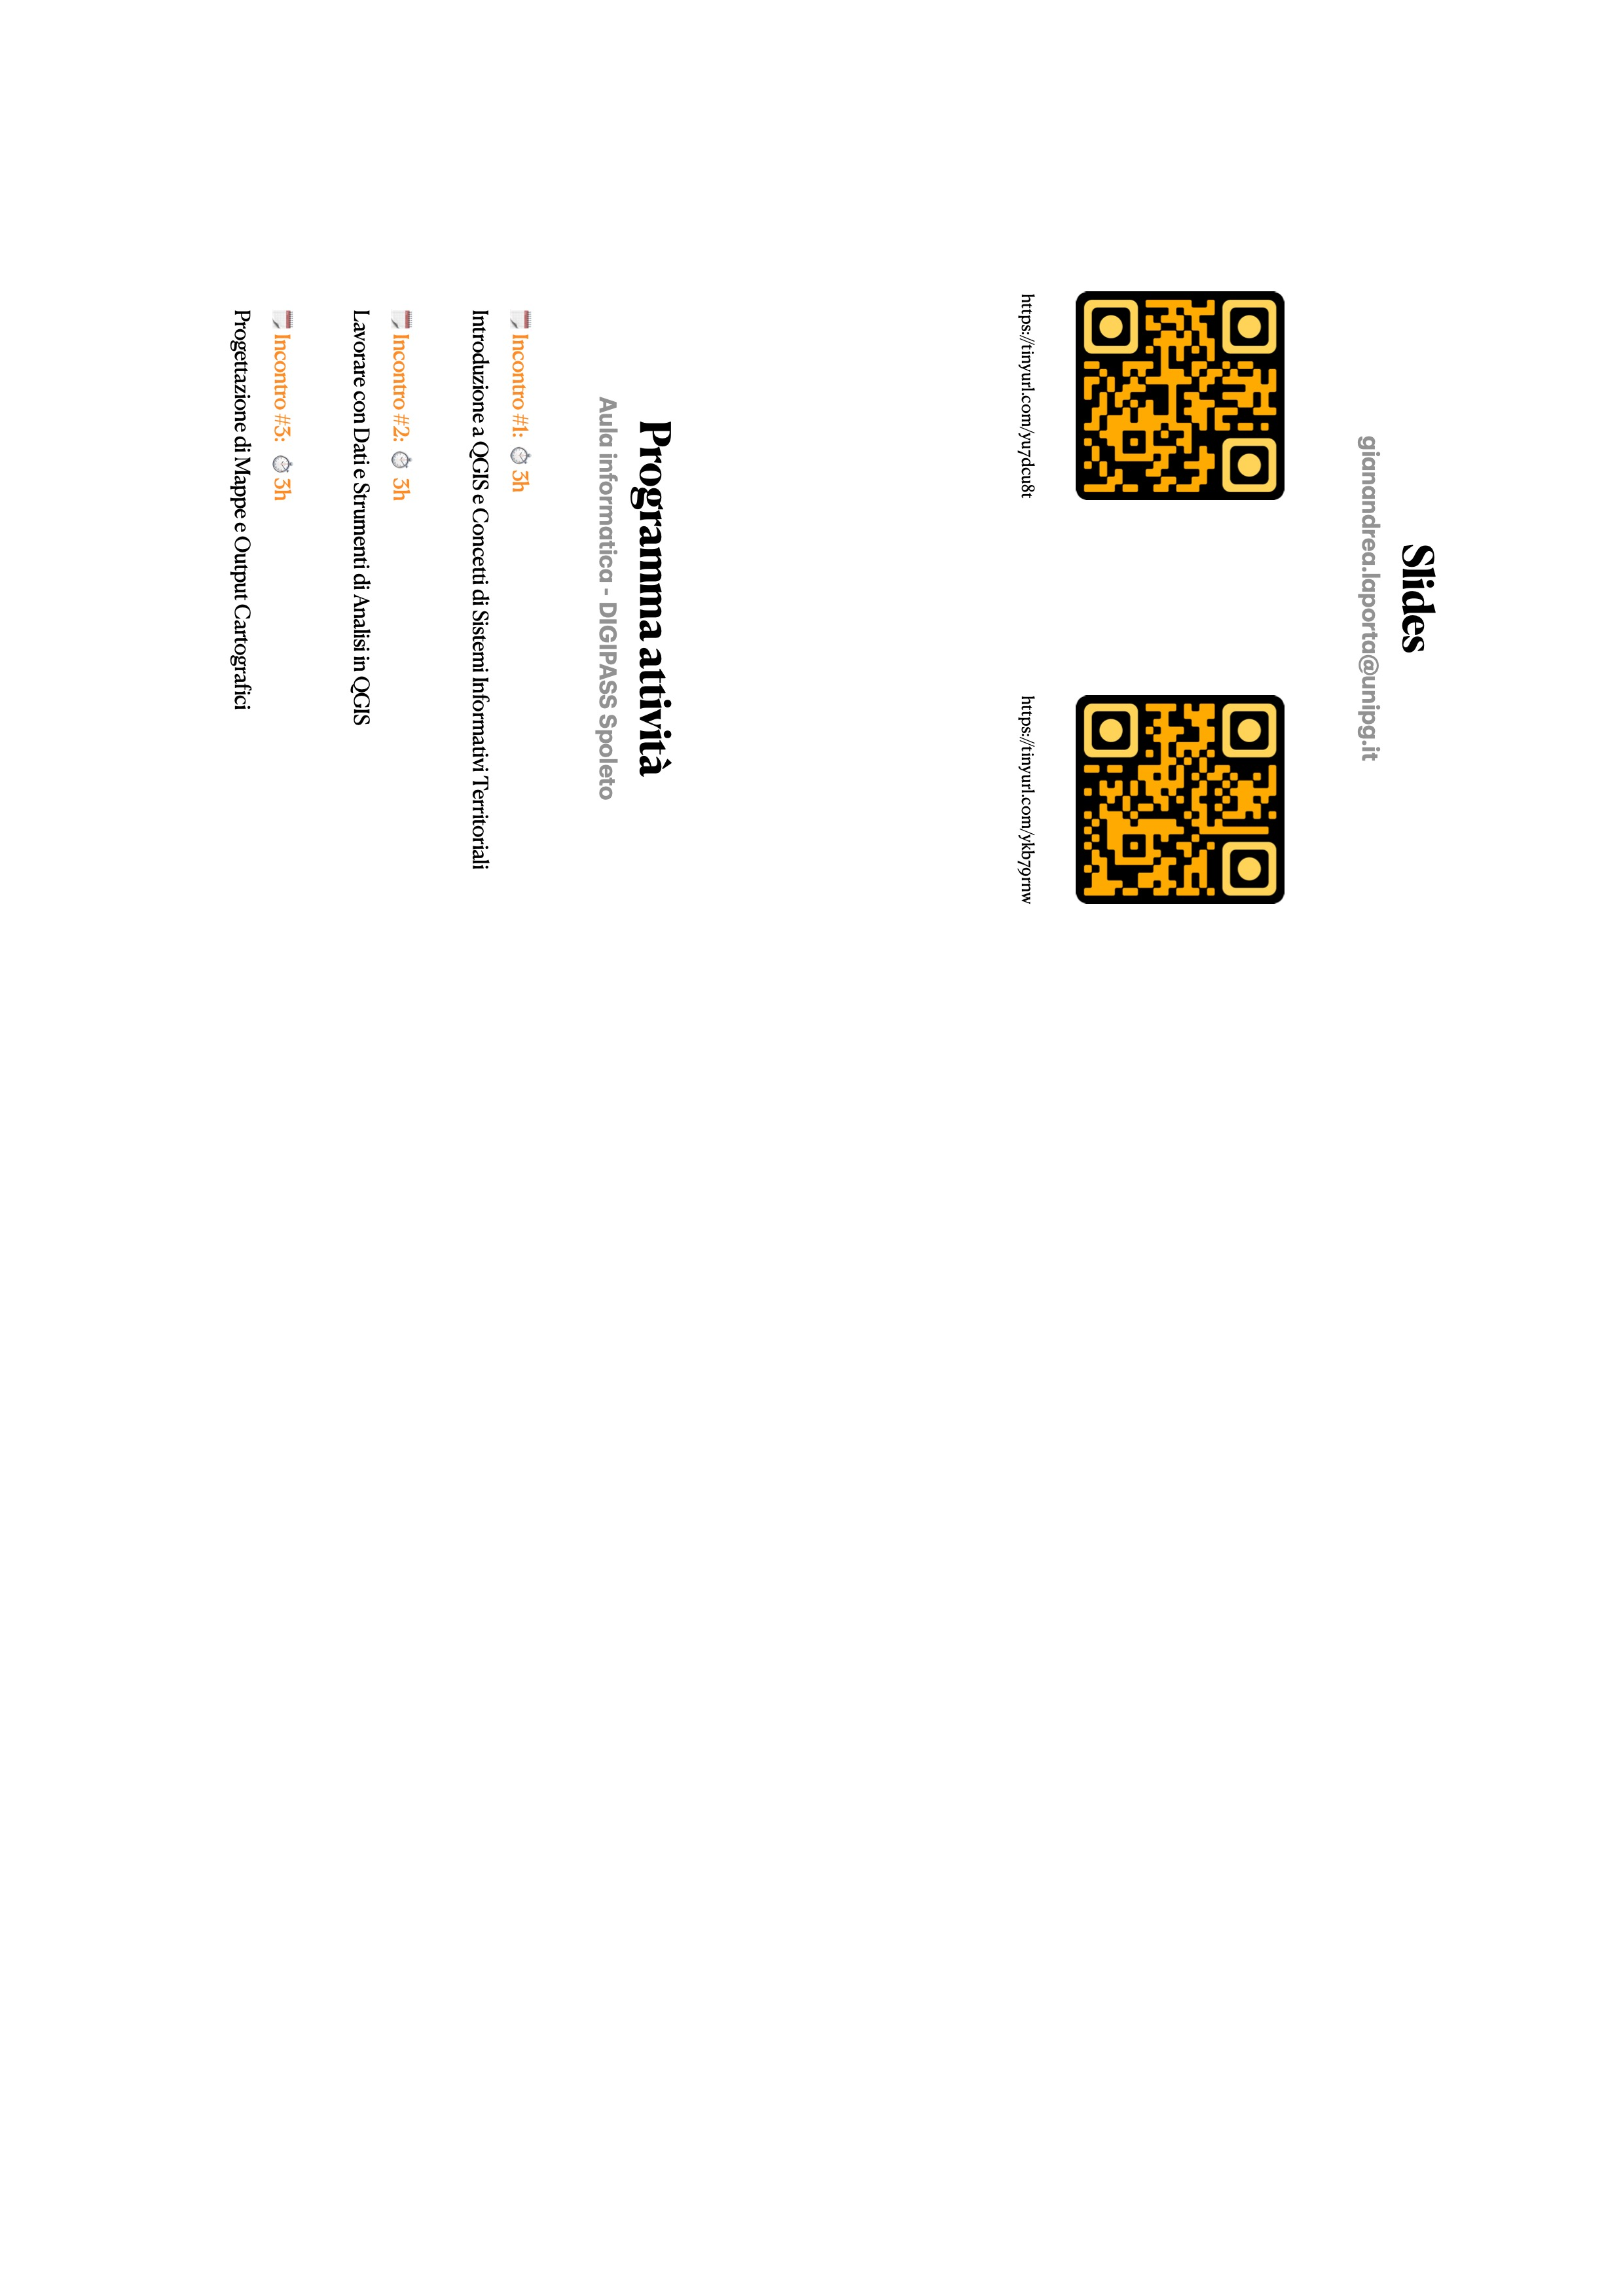
\includegraphics[keepaspectratio]{./figs/pctoREC/diversityRECSpoleto02 11-11.jpeg}}

\pandocbounded{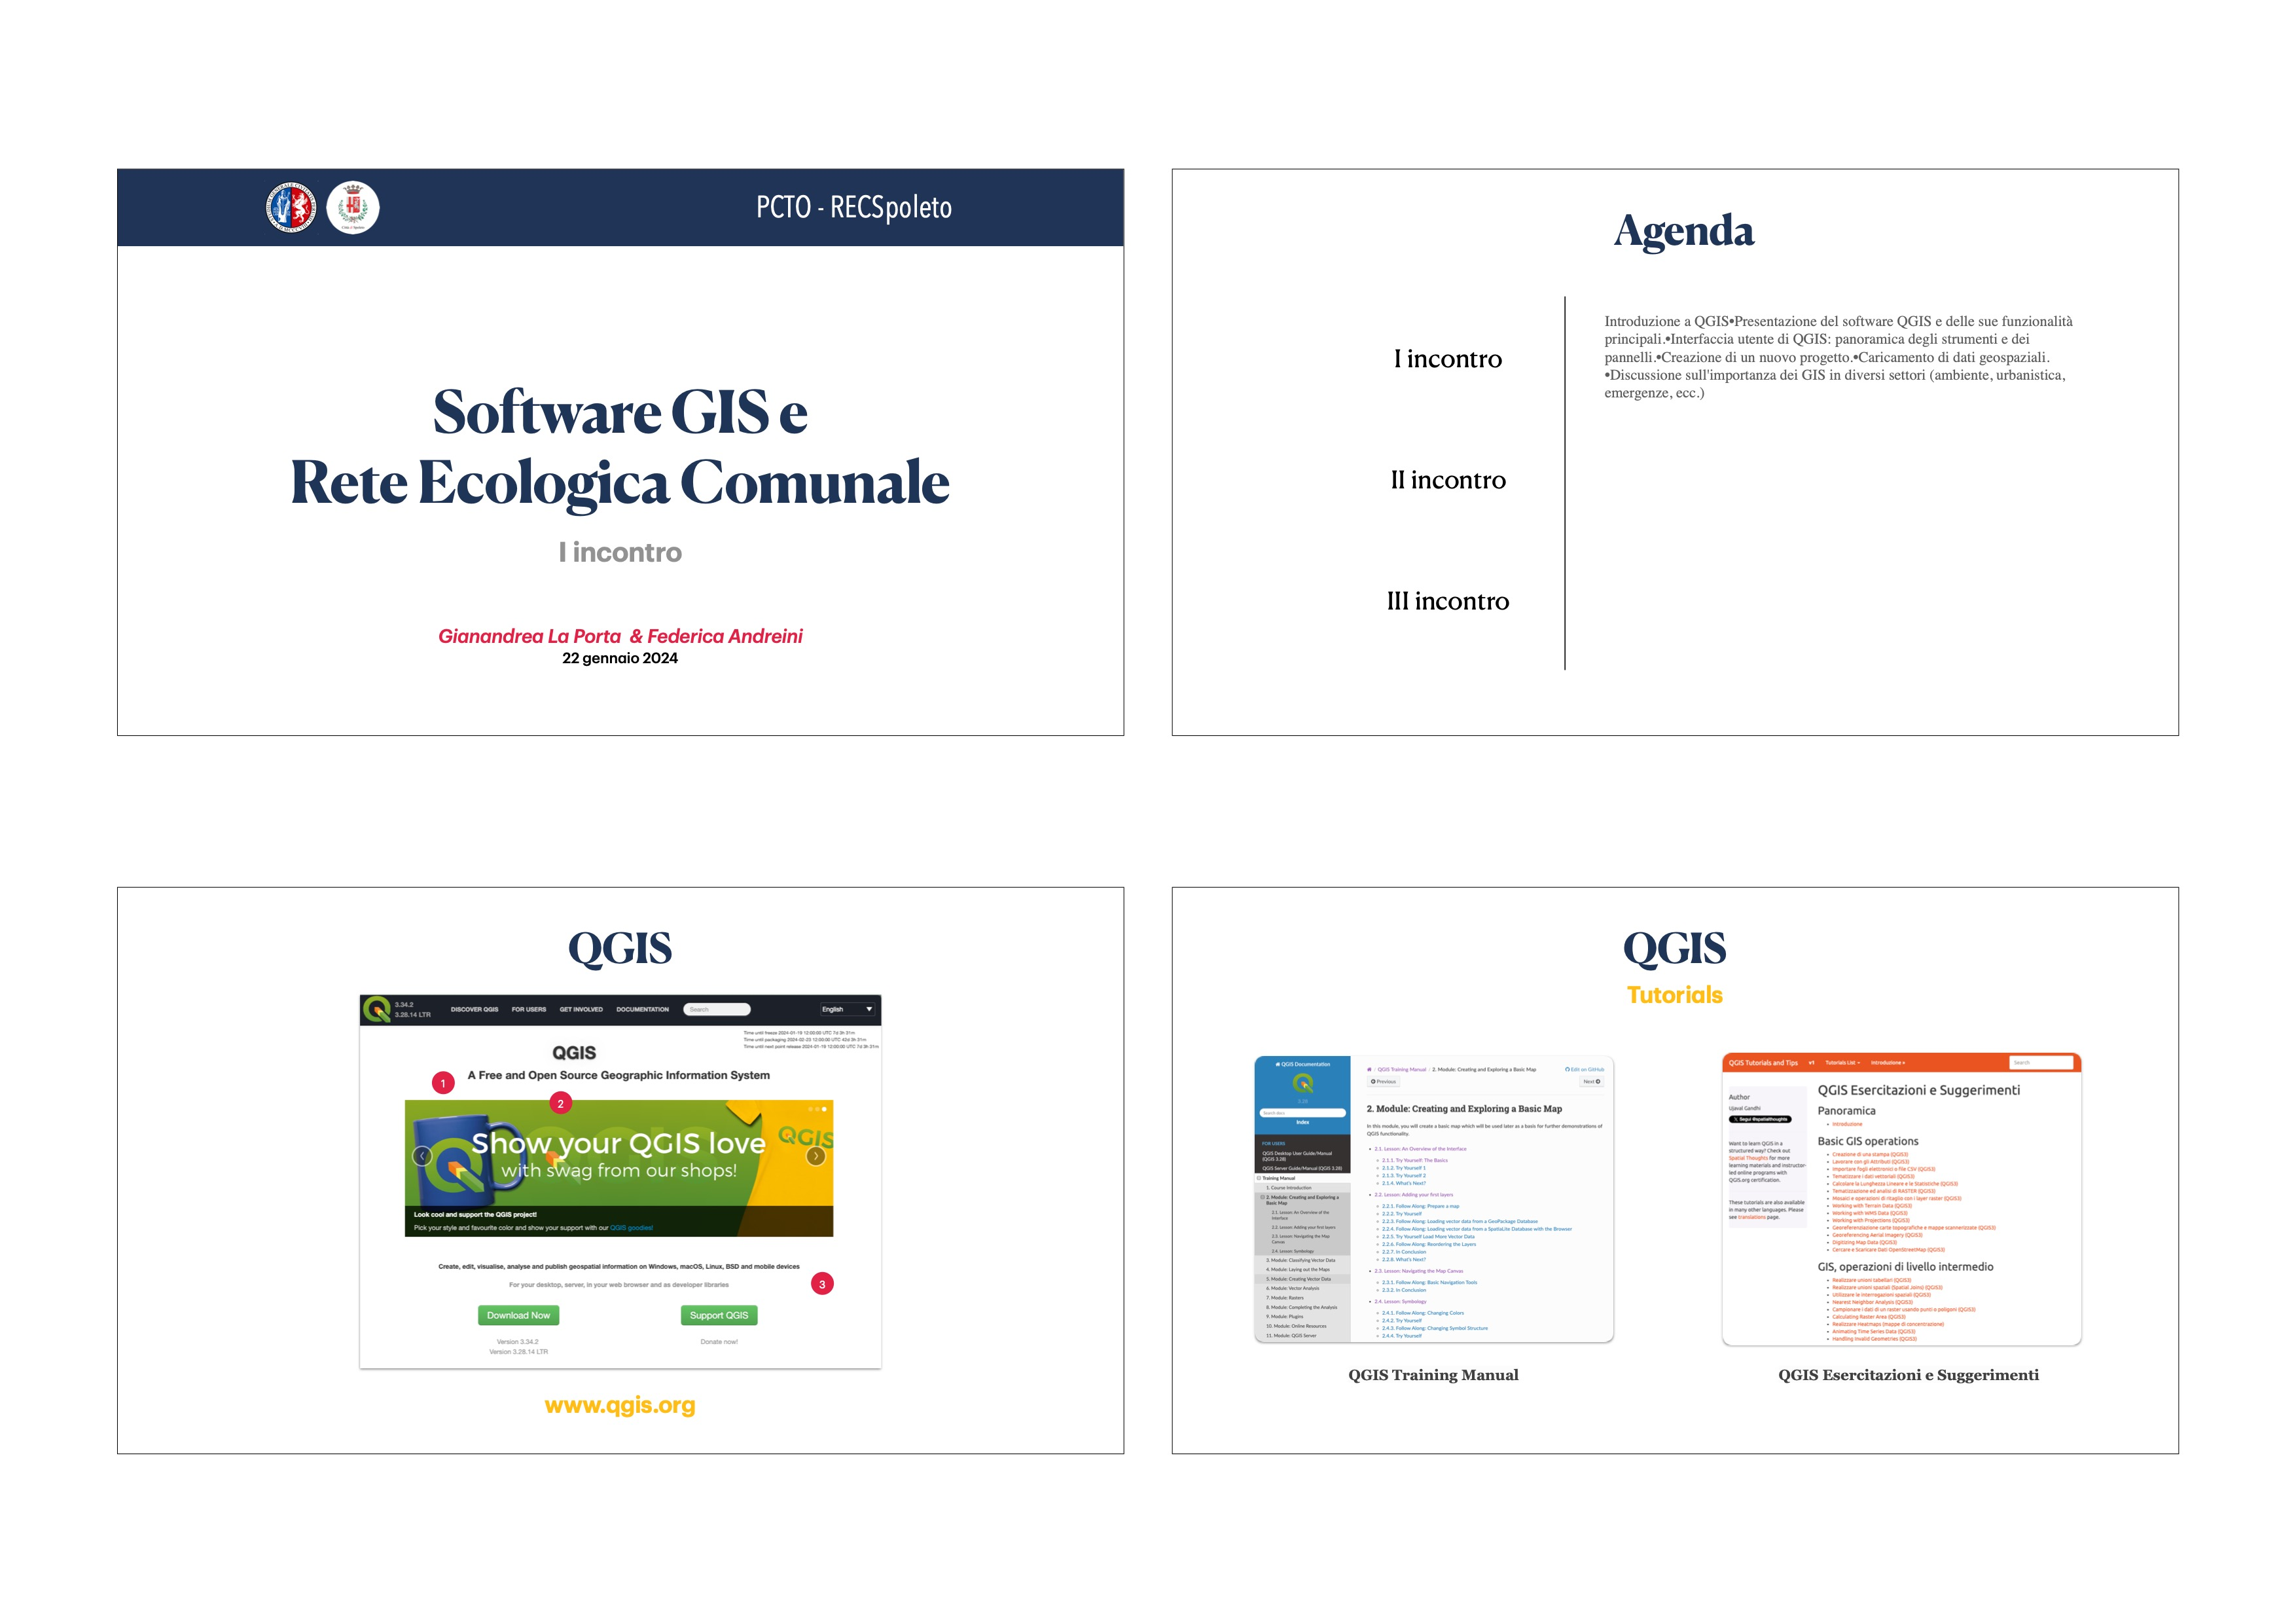
\includegraphics[keepaspectratio]{./figs/pctoGIS/RECSpoletoGISLect01-1.jpeg}}

\pandocbounded{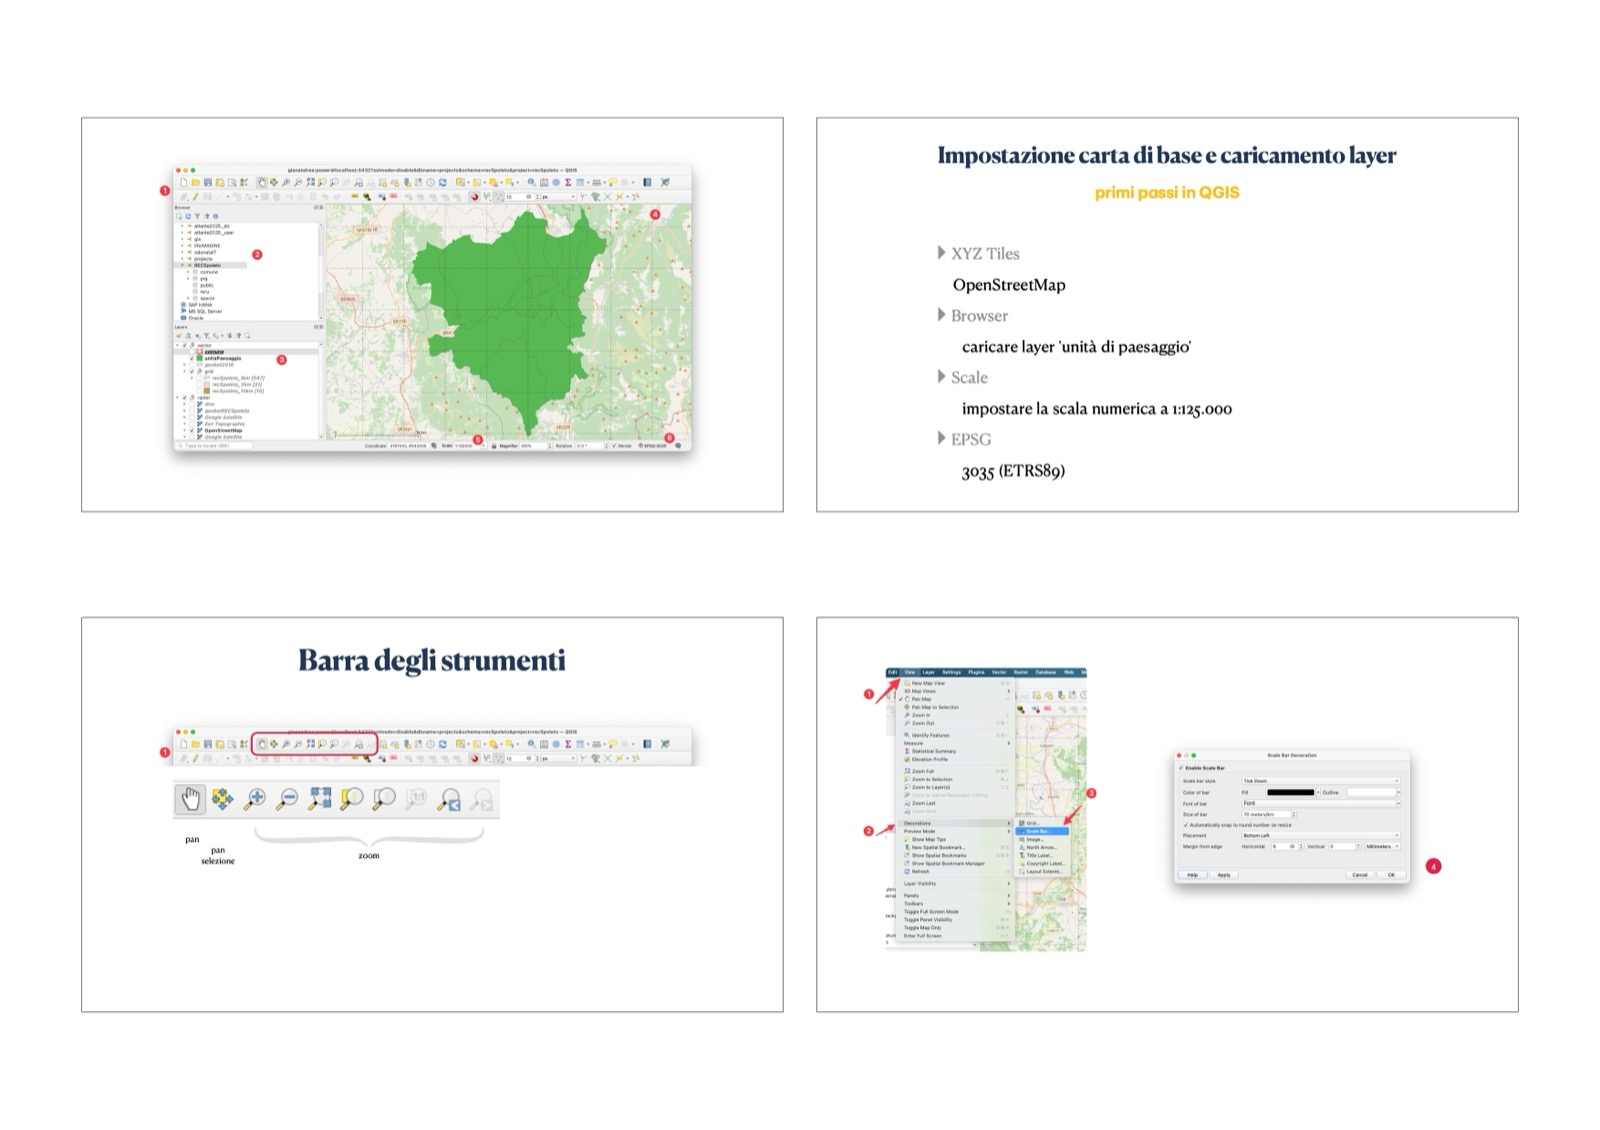
\includegraphics[keepaspectratio]{./figs/pctoGIS/RECSpoletoGISLect01 2-2.jpeg}}

\pandocbounded{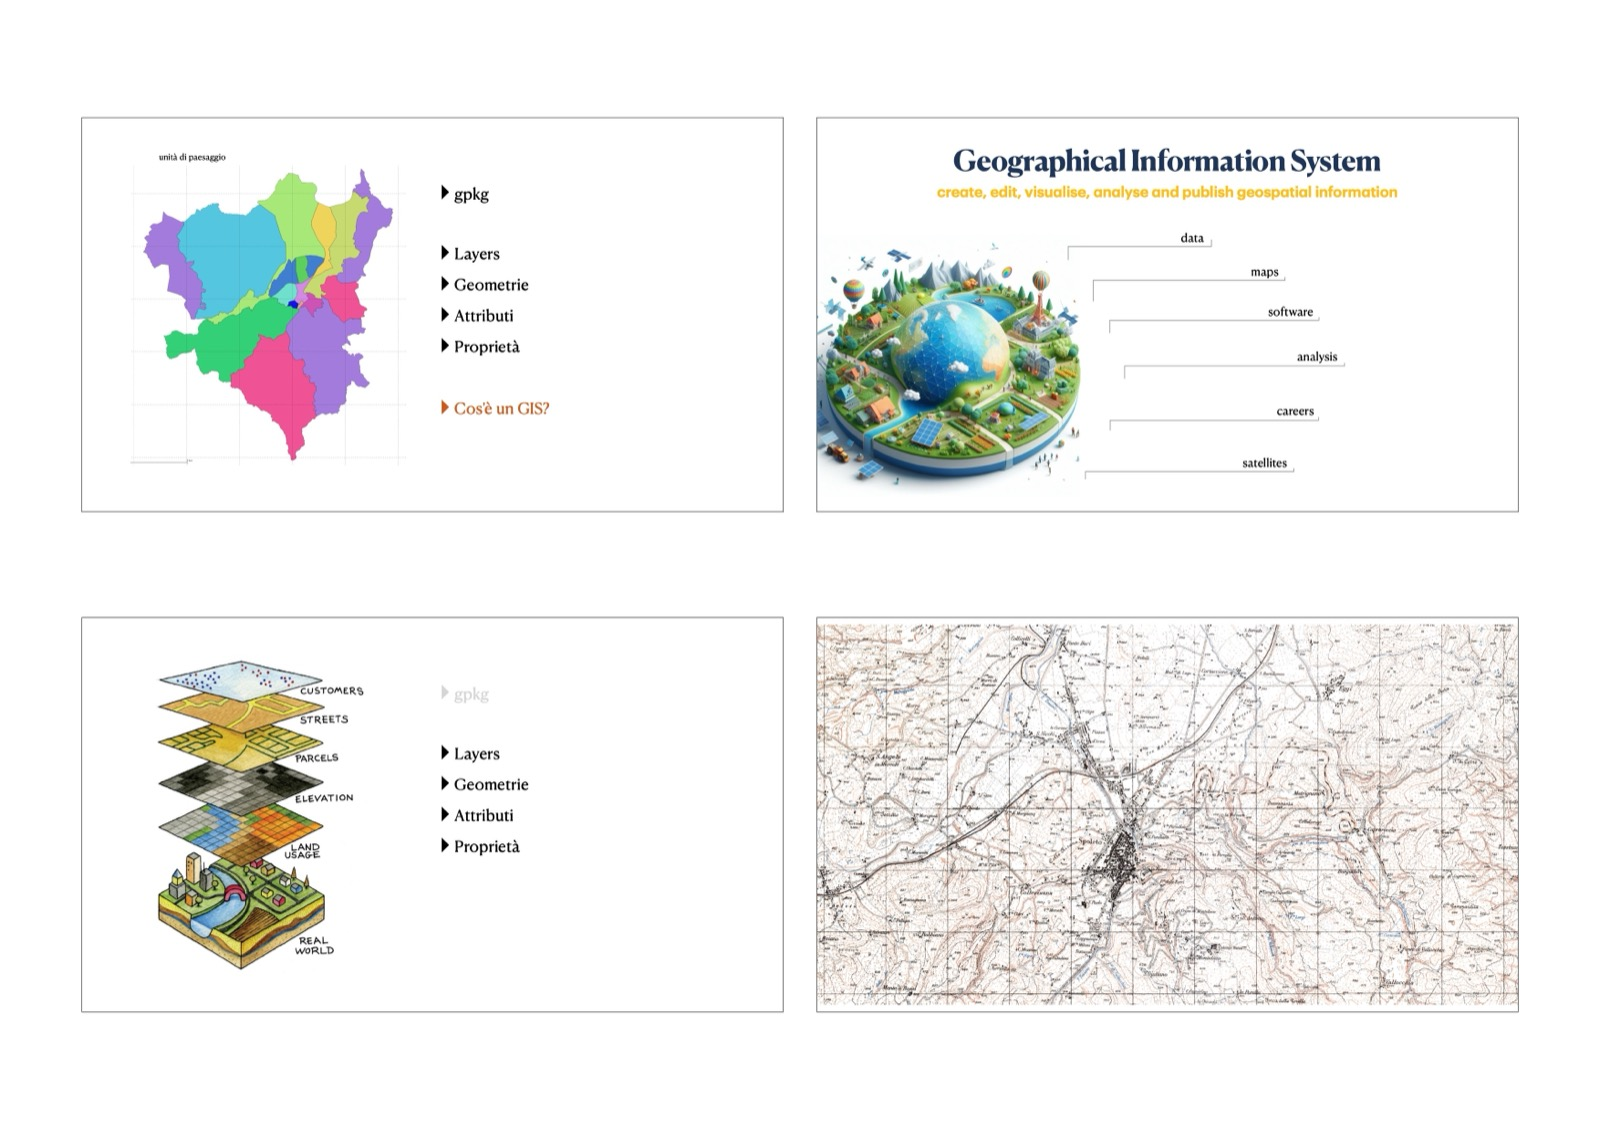
\includegraphics[keepaspectratio]{./figs/pctoGIS/RECSpoletoGISLect01 3-3.jpeg}}

\pandocbounded{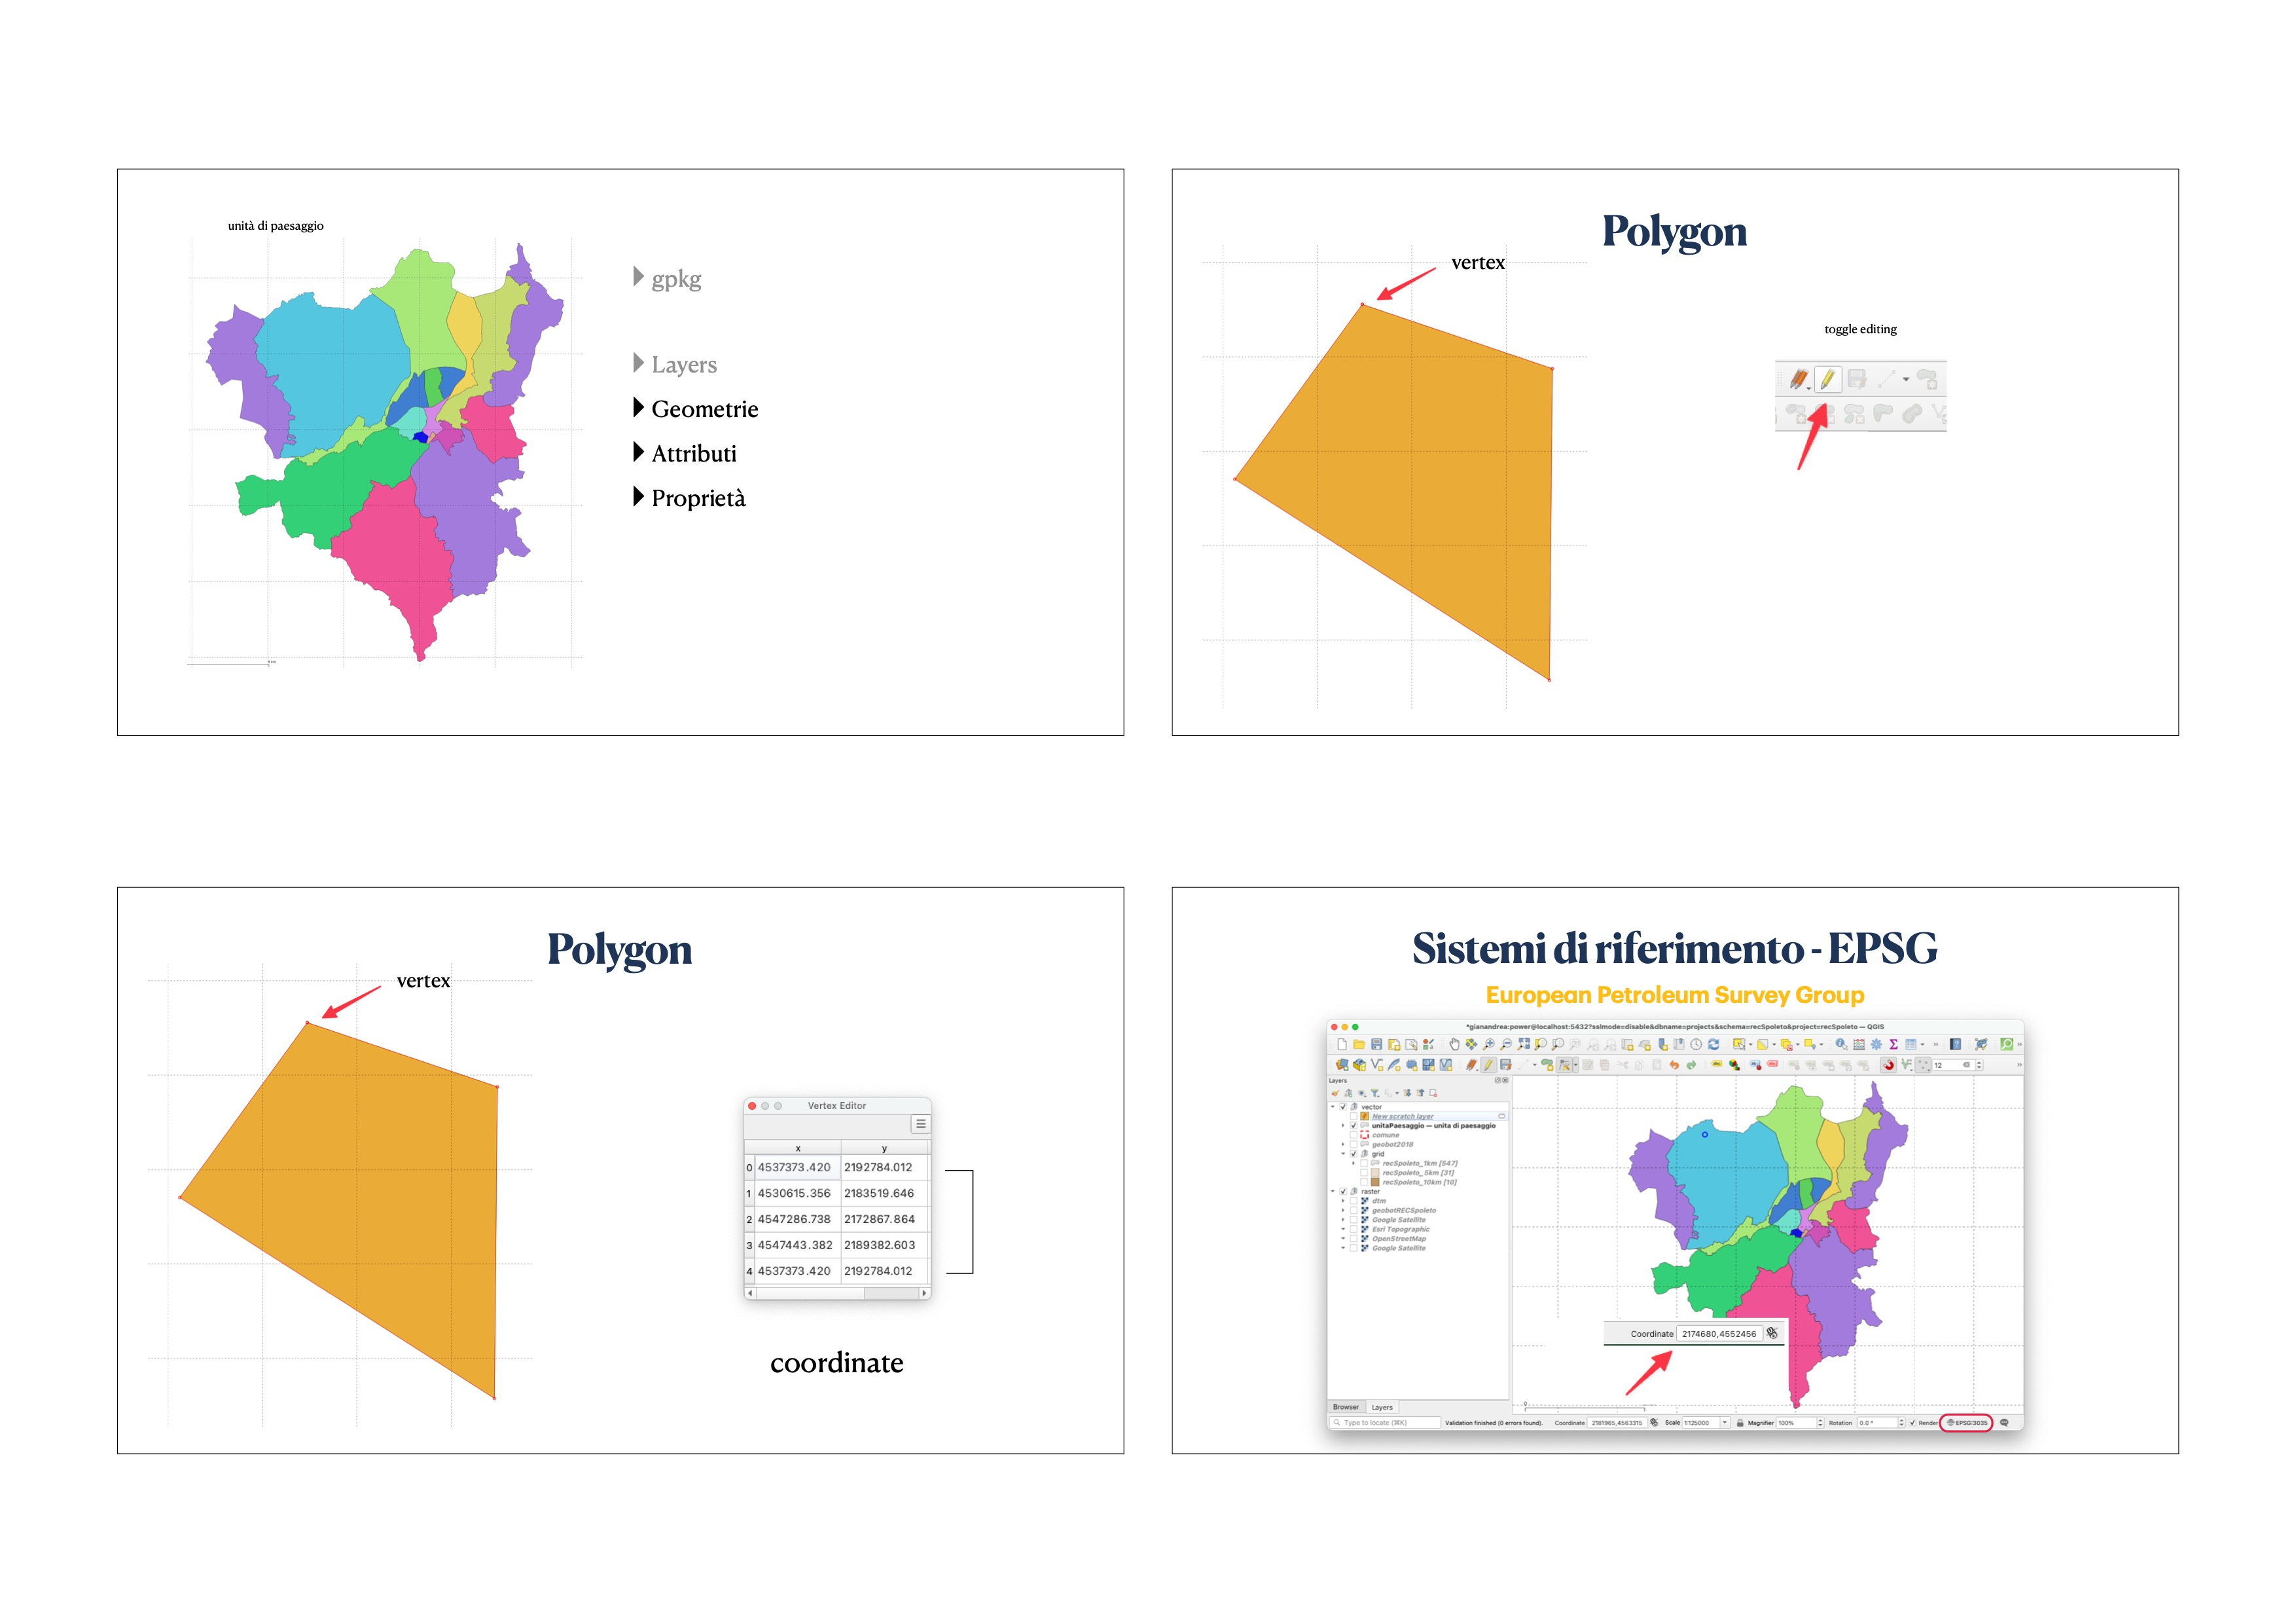
\includegraphics[keepaspectratio]{./figs/pctoGIS/RECSpoletoGISLect01 4-4.jpeg}}

\pandocbounded{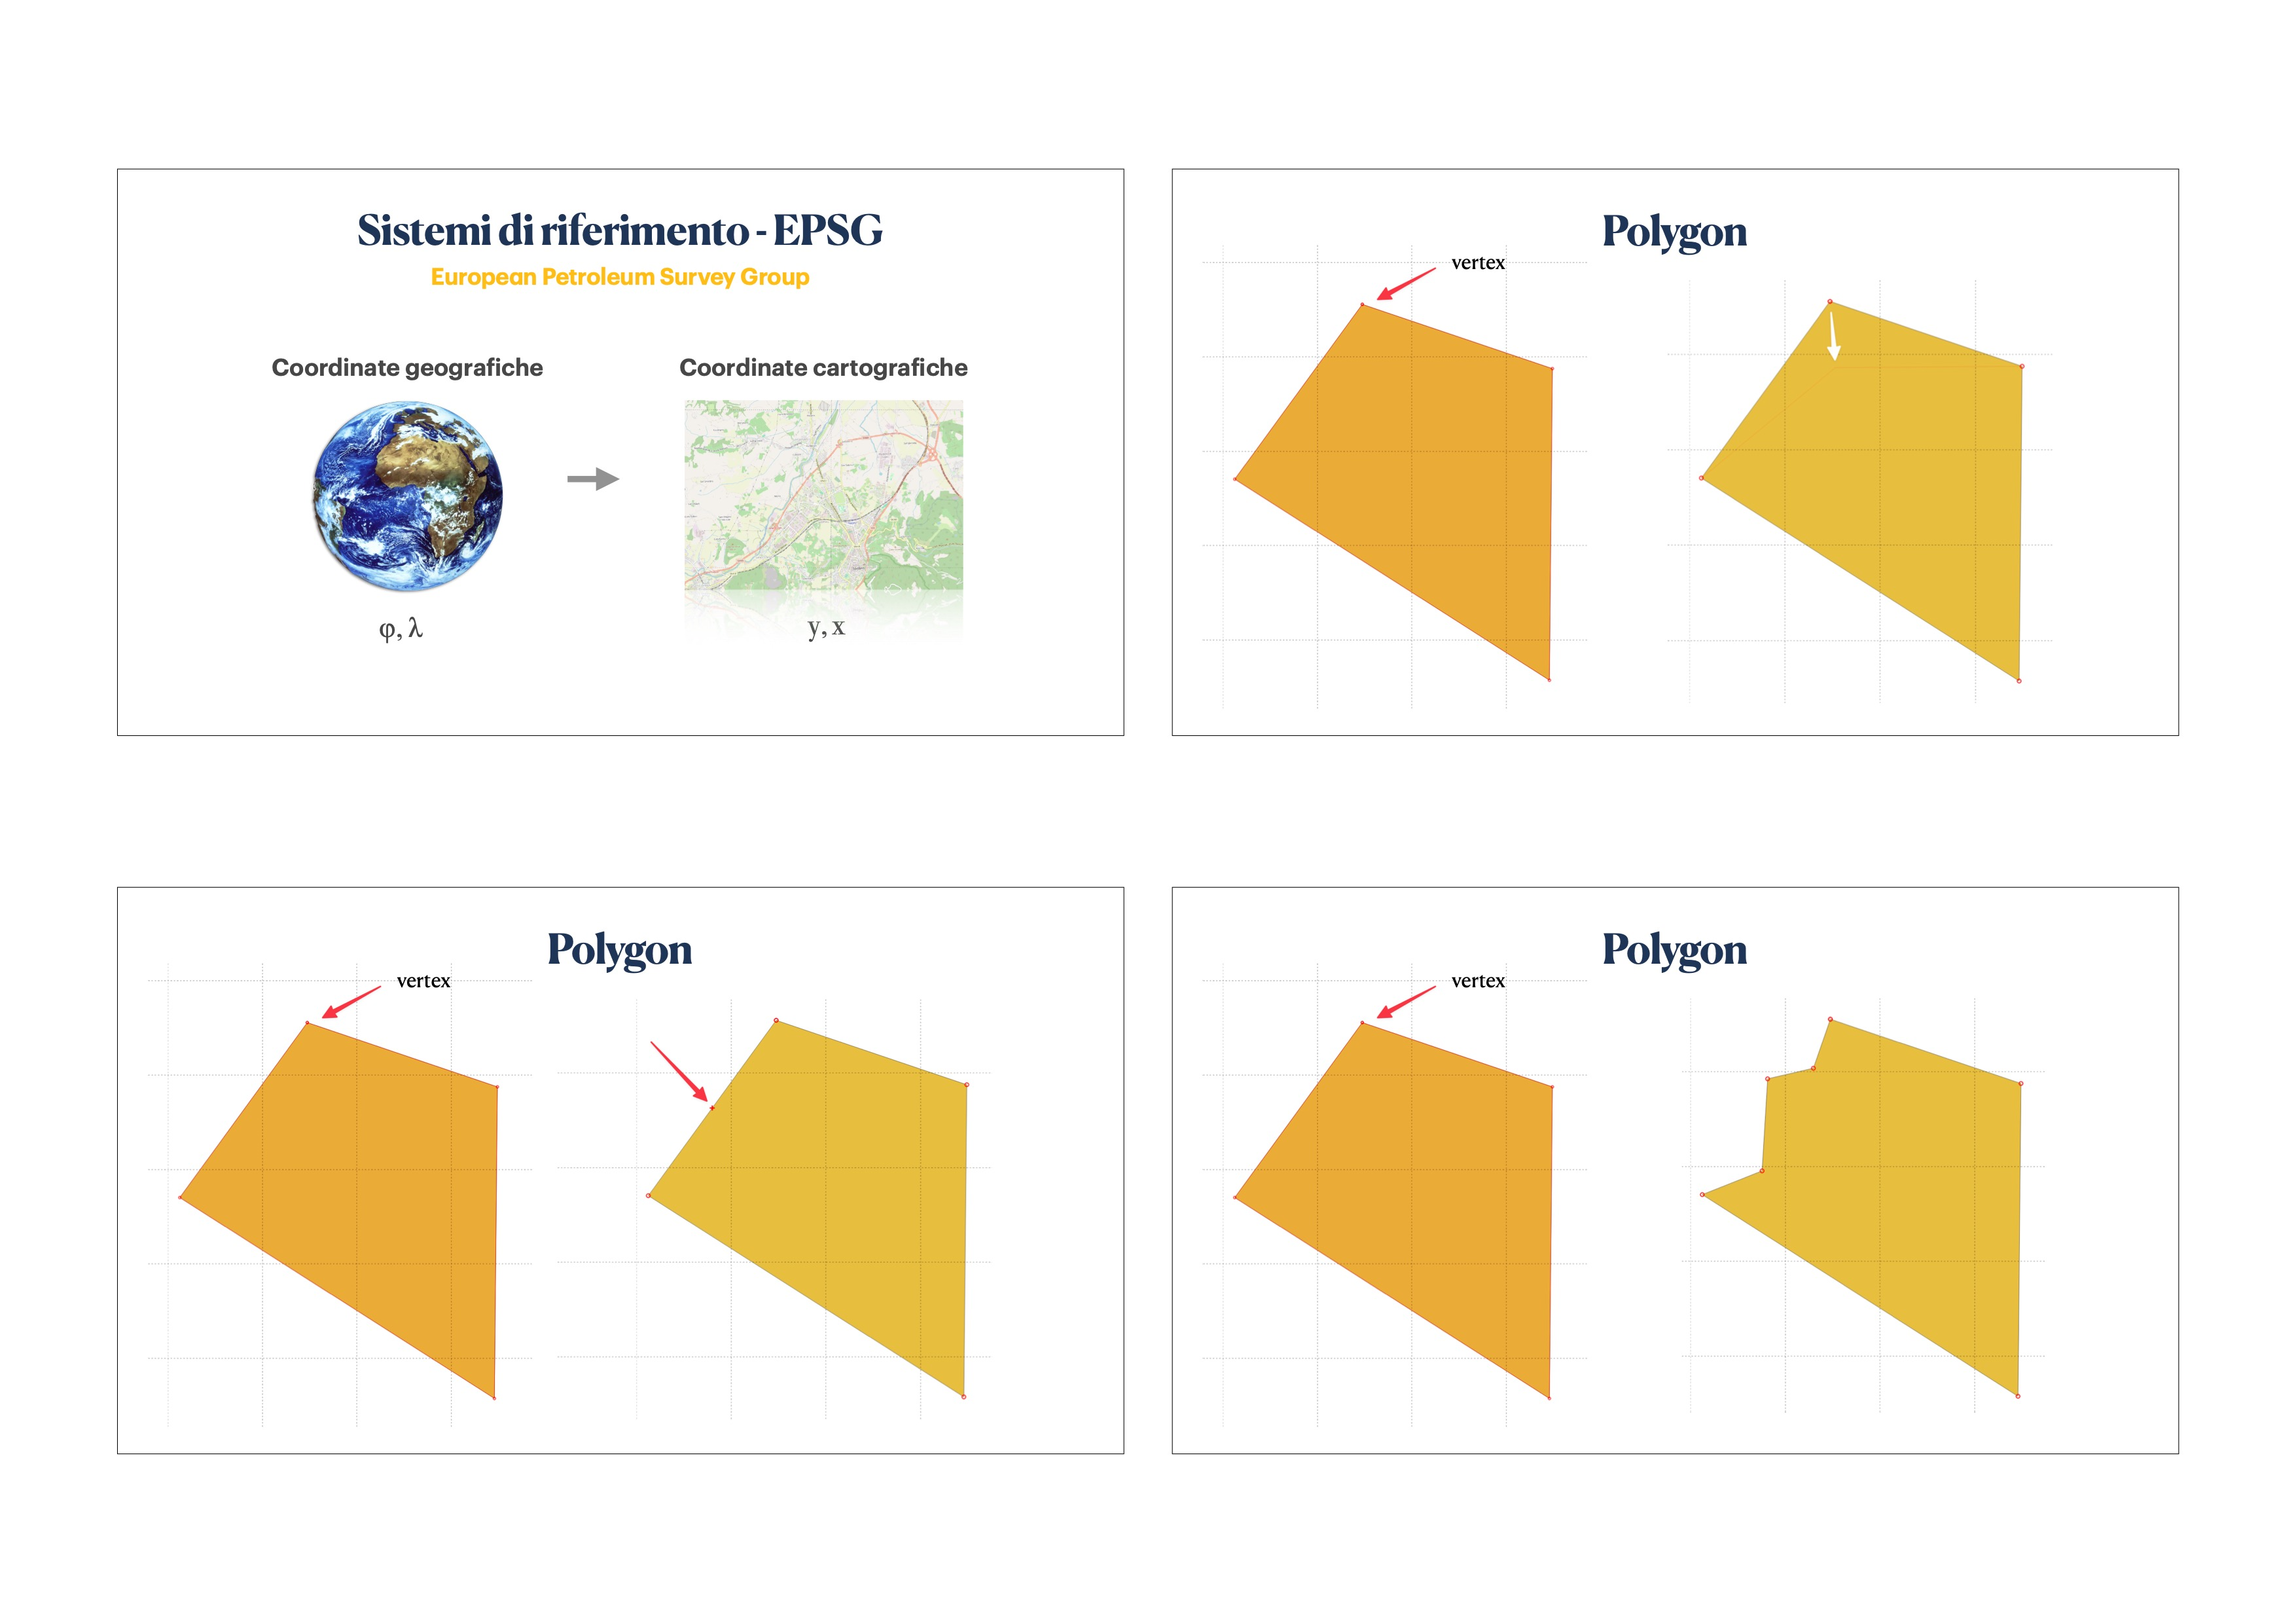
\includegraphics[keepaspectratio]{./figs/pctoGIS/RECSpoletoGISLect01 5-5.jpeg}}

\pandocbounded{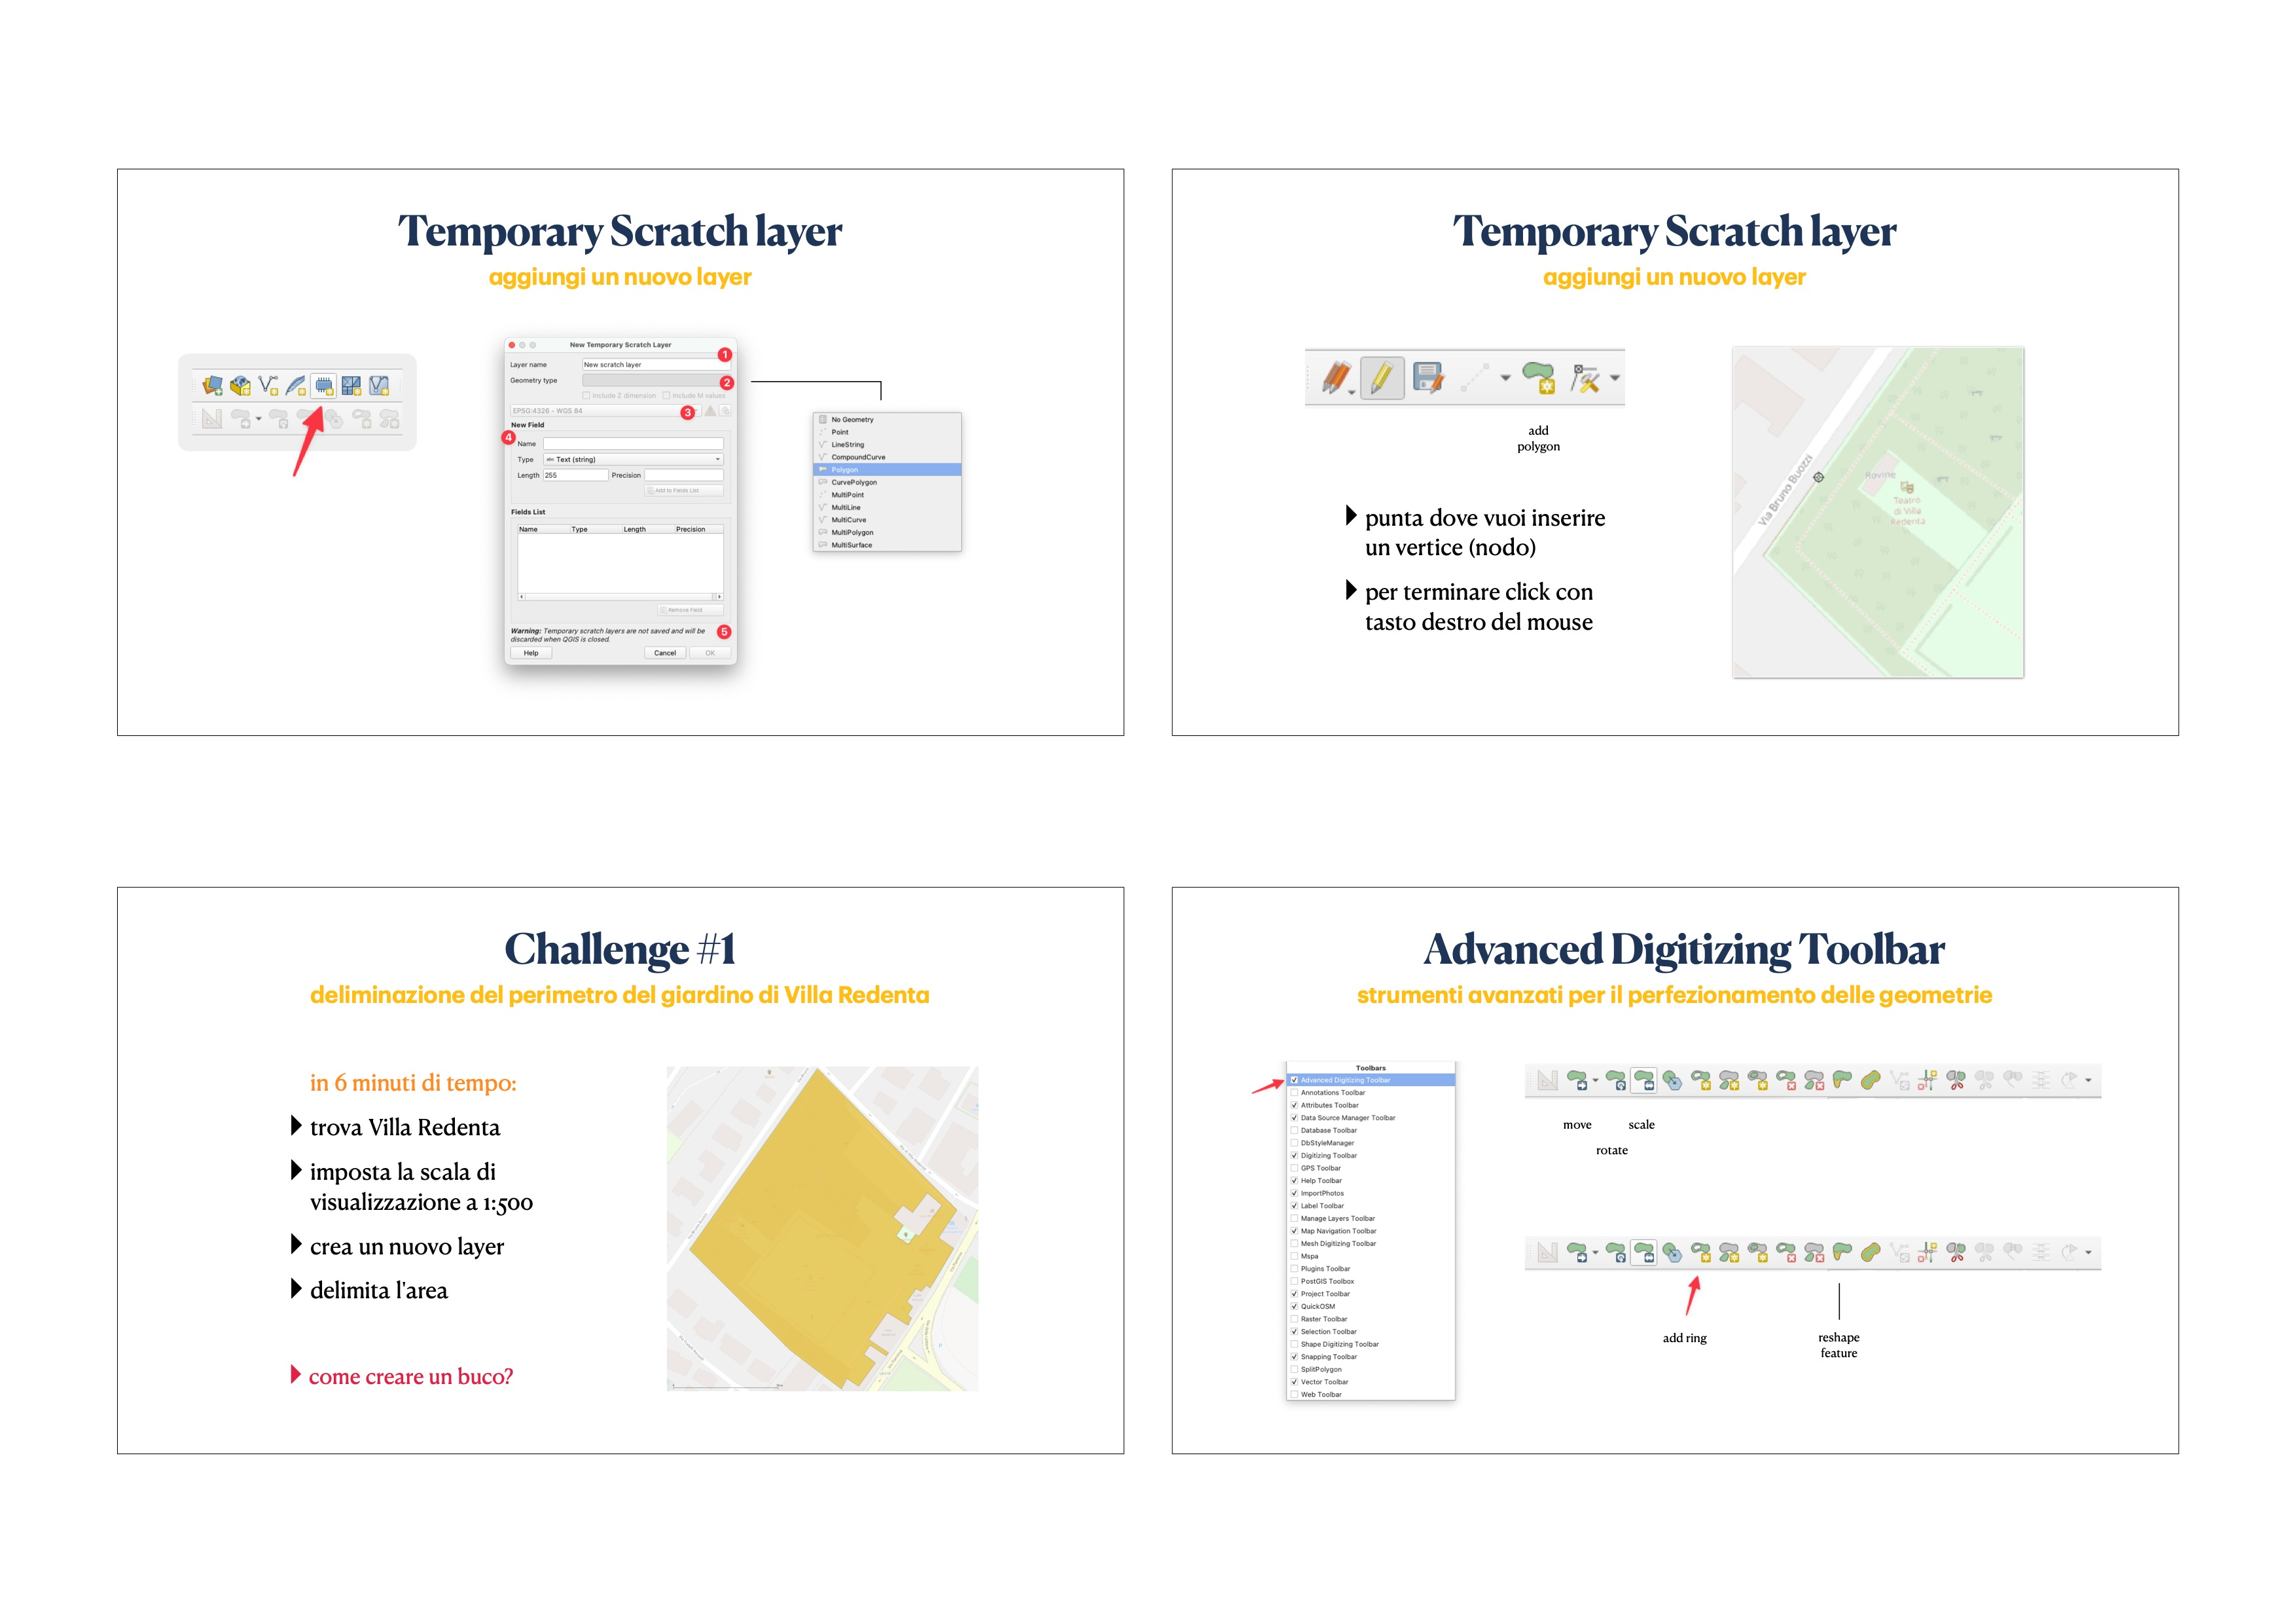
\includegraphics[keepaspectratio]{./figs/pctoGIS/RECSpoletoGISLect01 6-6.jpeg}}

\pandocbounded{\includegraphics[keepaspectratio]{./figs/pctoGIS/RECSpoletoGISLect01 7-7.jpeg}}

\pandocbounded{\includegraphics[keepaspectratio]{./figs/pctoGIS/RECSpoletoGISLect01 8-8.jpeg}}

\pandocbounded{\includegraphics[keepaspectratio]{./figs/pctoGIS/RECSpoletoGISLect01 9-9.jpeg}}

\pandocbounded{\includegraphics[keepaspectratio]{./figs/pctoGIS/RECSpoletoGISLect01 10-10.jpeg}}

\pandocbounded{\includegraphics[keepaspectratio]{./figs/pctoGIS/RECSpoletoGISLect01 11-11.jpeg}}

\pandocbounded{\includegraphics[keepaspectratio]{./figs/pctoGIS/RECSpoletoGISLect02-1.jpeg}}

\pandocbounded{\includegraphics[keepaspectratio]{./figs/pctoGIS/RECSpoletoGISLect02 2-2.jpeg}}

\pandocbounded{\includegraphics[keepaspectratio]{./figs/pctoGIS/RECSpoletoGISLect02 3-3.jpeg}}

\pandocbounded{\includegraphics[keepaspectratio]{./figs/pctoGIS/RECSpoletoGISLect02 4-4.jpeg}}

\pandocbounded{\includegraphics[keepaspectratio]{./figs/pctoGIS/RECSpoletoGISLect02 5-5.jpeg}}

\pandocbounded{\includegraphics[keepaspectratio]{./figs/pctoGIS/RECSpoletoGISLect02 6-6.jpeg}}

\pandocbounded{\includegraphics[keepaspectratio]{./figs/pctoGIS/RECSpoletoGISLect02 7-7.jpeg}}

\pandocbounded{\includegraphics[keepaspectratio]{./figs/pctoGIS/RECSpoletoGISLect02 8-8.jpeg}}

\pandocbounded{\includegraphics[keepaspectratio]{./figs/pctoGIS/RECSpoletoGISLect02 9-9.jpeg}}

\pandocbounded{\includegraphics[keepaspectratio]{./figs/pctoGIS/RECSpoletoGISLect02 10-10.jpeg}}

\pandocbounded{\includegraphics[keepaspectratio]{./figs/pctoGIS/RECSpoletoGISLect03-1.jpeg}}

\pandocbounded{\includegraphics[keepaspectratio]{./figs/pctoGIS/RECSpoletoGISLect03 2-2.jpeg}}

\pandocbounded{\includegraphics[keepaspectratio]{./figs/pctoGIS/RECSpoletoGISLect03 3-3.jpeg}}

\pandocbounded{\includegraphics[keepaspectratio]{./figs/pctoGIS/RECSpoletoGISLect03 4-4.jpeg}}

\pandocbounded{\includegraphics[keepaspectratio]{./figs/pctoGIS/RECSpoletoGISLect03 5-5.jpeg}}

\pandocbounded{\includegraphics[keepaspectratio]{./figs/pctoGIS/RECSpoletoGISLect03 6-6.jpeg}}

\pandocbounded{\includegraphics[keepaspectratio]{./figs/pctoGIS/RECSpoletoGISLect03 7-7.jpeg}}

\pandocbounded{\includegraphics[keepaspectratio]{./figs/pctoGIS/RECSpoletoGISLect03 8-8.jpeg}}

\subsection{Incontro pubblico: Diventare un citizen scientist monitoraggio della fauna minore}\label{incontro-pubblico-diventare-un-citizen-scientist-monitoraggio-della-fauna-minore}

\pandocbounded{\includegraphics[keepaspectratio]{./figs/CSSpoleto/CSSpoletoLaPorta20240726-1.jpeg}}

\pandocbounded{\includegraphics[keepaspectratio]{./figs/CSSpoleto/CSSpoletoLaPorta20240726 2-2.jpeg}}

\pandocbounded{\includegraphics[keepaspectratio]{./figs/CSSpoleto/CSSpoletoLaPorta20240726 3-3.jpeg}}

\pandocbounded{\includegraphics[keepaspectratio]{./figs/CSSpoleto/CSSpoletoLaPorta20240726 4-4.jpeg}}

\pandocbounded{\includegraphics[keepaspectratio]{./figs/CSSpoleto/CSSpoletoLaPorta20240726 5-5.jpeg}}
\pandocbounded{\includegraphics[keepaspectratio]{./figs/CSSpoleto/CSSpoletoLaPorta20240726 6-6.jpeg}}

\subsection{Convegno Fauna 2024 con contributo dal titolo: La conservazione delle libellule nelle campagne}\label{convegno-fauna-2024-con-contributo-dal-titolo-la-conservazione-delle-libellule-nelle-campagne}

\pandocbounded{\includegraphics[keepaspectratio]{./figs/Fauna2024/fauna2024-1.jpeg}}

\pandocbounded{\includegraphics[keepaspectratio]{./figs/Fauna2024/fauna2024-2.jpeg}}

\pandocbounded{\includegraphics[keepaspectratio]{./figs/Fauna2024/fauna2024-3.jpeg}}

\pandocbounded{\includegraphics[keepaspectratio]{./figs/Fauna2024/fauna2024-4.jpeg}}

\pandocbounded{\includegraphics[keepaspectratio]{./figs/Fauna2024/fauna2024-5.jpeg}}

\pandocbounded{\includegraphics[keepaspectratio]{./figs/Fauna2024/fauna2024-6.jpeg}}

\pandocbounded{\includegraphics[keepaspectratio]{./figs/Fauna2024/fauna2024-7.jpeg}}

\subsection{Convegno Fauna 2025 con contributo dal titolo: Fauna e Reti ecologiche: progettare connessioni per la biodiversità}\label{convegno-fauna-2025-con-contributo-dal-titolo-fauna-e-reti-ecologiche-progettare-connessioni-per-la-biodiversituxe0}

\pandocbounded{\includegraphics[keepaspectratio]{./figs/Fauna2025/fauna2025.key 1.jpeg}}

\pandocbounded{\includegraphics[keepaspectratio]{./figs/Fauna2025/fauna2025.key 2.jpeg}}

\pandocbounded{\includegraphics[keepaspectratio]{./figs/Fauna2025/fauna2025.key 3.jpeg}}

\pandocbounded{\includegraphics[keepaspectratio]{./figs/Fauna2025/fauna2025.key 4.jpeg}}

\pandocbounded{\includegraphics[keepaspectratio]{./figs/Fauna2025/fauna2025.key 5.jpeg}}

\pandocbounded{\includegraphics[keepaspectratio]{./figs/Fauna2025/fauna2025.key 6.jpeg}}

\pandocbounded{\includegraphics[keepaspectratio]{./figs/Fauna2025/fauna2025.key 7.jpeg}}

\pandocbounded{\includegraphics[keepaspectratio]{./figs/Fauna2025/fauna2025.key 8.jpeg}}

\pandocbounded{\includegraphics[keepaspectratio]{./figs/Fauna2025/fauna2025.key 9.jpeg}}

\pandocbounded{\includegraphics[keepaspectratio]{./figs/Fauna2025/fauna2025.key 10.jpeg}}

\end{document}
